\documentclass[a4paper, 12pt]{article} 

%load any additional packages
\usepackage{amssymb}
\usepackage{graphicx}
\usepackage[numbers]{natbib}
%\usepackage{biblatex}
\usepackage{multicol}
\usepackage{setspace} 
\usepackage{fancyhdr}
\usepackage{times}
\usepackage{tocloft}
\usepackage{geometry}
\usepackage{textcomp}
\usepackage{comment}
\usepackage{enumitem}
\usepackage{amsmath}

\usepackage{color}
\usepackage{tcolorbox}
\usepackage{listings}

\usepackage{float}
\usepackage{caption}
\usepackage{multirow}

\usepackage{xcolor}
\usepackage{xcolor}
\usepackage{tocloft}
\usepackage{titling}
\definecolor{myblue}{RGB}{0, 0, 255}

% Set basic style for listings
\lstset{basicstyle=\ttfamily\small\color{black}, 
        breaklines=true % Allow line breaks
        }

\renewcommand{\contentsname}{%
  \hfill\bfseries\Large\color{myblue}\underline{Table of Content}\hfill}

% Redefine \section to include color
\usepackage{titlesec}
\titleformat{\section}
  {\color{blue}\normalfont\Large\bfseries} % Format section headings
  {\thesection}{1em}{}


\renewcommand{\headrulewidth}{0pt}% for removing the line under header 
\fancyhead{} %remove section number from header 
%\clearpage

\usepackage[hidelinks]{hyperref}
\usepackage{siunitx} % Required for alignment
\sisetup{
  round-mode          = places, % Rounds numbers
  round-precision     = 2, % to 2 places
}
\geometry{a4paper,total={175mm,257mm},left=25mm,right=25mm,top=30mm, bottom=30mm}
\hypersetup{
    colorlinks=true,    % Enable colored links
    linkcolor=black,     % Color for internal links
    filecolor=magenta,  % Color for file links
    urlcolor=blue,       % Color for URLs
    citecolor=blue      % colour for cite  
}
% Set citation style to square brackets
\setcitestyle{square}
% \setcounter{chapter}{1}
\renewcommand{\cftsecleader}{\cftdotfill{\cftdotsep}} % Default dots

% Define a custom command to add section numbers
\newcommand{\sectionnumber}{\arabic{section}}


% Add project title here
\def\mytitle{\fontsize{28}{30}\selectfont{Analyzing Social Media Posts for Mental Health Disorder Detection}}

% Add student Degree
\def\mydegree{Bachelor of Technology}
% Add student \textbf{name}
\def\mysupervisor{Nairanjana Chowdhury}
% Supervisor designation : Assistant Professor, Associate Professor, Professor
\def\mysupervisordesig{Professor}

% Add student names and roll no
\def\mynameone{SOUMYADEEP NANDY}
\def\myrollnoone{13000121033}
\def\mynametwo{PRITHWISH SARKAR}
\def\myrollnotwo{13000121037}
\def\mynamethree{SAGNIK MUKHOPADHYAY}
\def\myrollnothree{13000121040}
\def\mynamefour{ARKAPRATIM GHOSH}
\def\myrollnofour{13000121058}

% Add student department
\def\mydep{Computer Science and Engineering}
\def\myHODname{Dr. Tapan Chowdhury}
% HOD designation : Assistant Professor, Associate Professor, Professor
\def\myHODdesig{Professor}
% Add the date of submission
\def\mydegreedate{\today}

\begin{document}
 \baselineskip=18pt plus1pt
 \setcounter{secnumdepth}{4}
%  \setcounter{secnumdepth}{3}
 \setcounter{tocdepth}{4}
 \pagenumbering{roman}
 \pagenumbering{roman}

 \graphicspath{ {./Images/} }
 %Front Matter
 \thispagestyle{empty}
\begin{center}
    { \Large {\bfseries {\mytitle}} \par}
\vspace{2\baselineskip}
    {
    %\textit{Thesis to be submitted in partial fulfillment of the}\\
    \large{Submitted by} 
    
    \vspace{2\baselineskip}
   % \large{.. \textlangle{}Name and Roll Number\textrangle{} ..} 

\vspace{\baselineskip}

    {SOUMYADEEP NANDY (13000121033)}
    
    \vspace{\baselineskip}

   {PRITHWISH SARKAR (13000121037)}
  \vspace{\baselineskip}

     {SAGNIK MUKHOPADHYAY (13000121040)}
    \vspace{\baselineskip}

    {ARKAPRATIM GHOSH (13000121058)}

\vspace{1\baselineskip}
%\vspace{-0.1\baselineskip}
%    {{\large {\bf \myrollno}} \par}
% \vspace{1.5\baselineskip}
%     {Under the guidance of \par}
% \vspace{\baselineskip}
%     {{\large \bf \mysupervisor} \par}
\vspace{1\baselineskip}
    \large{ \textlangle{} Group 29 \textrangle{}}}
    
 \vspace{1\baselineskip}   
    \large{Final Year 7\textsuperscript{th} Semester \par}   
\vspace{\baselineskip}
    \large{ \textlangle{} September, 2024 \textrangle{}}
    
\vspace{\baselineskip}
   % \large
    {\ {Submitted for the partial fulfillment for the degree of \\Bachelor of Technology in \\Computer Science and Engineering }\par}
\vspace{1\baselineskip}
    {\begin{figure}[!h] 
	\centering
	
\includegraphics[width=30mm]{./Images/tmsl.png} 
     \end{figure}
    }
%{\large \vspace*{1ex}
\vspace{1.5\baselineskip}

    { {Techno Main Salt Lake,\\
                    EM 4/1, Salt lake, Sector - V, Kolkata - 700091} \par}
 \end{center}
 \thispagestyle{plain}

% \begin{multicols}{1}
 % \flushleft
 % \includegraphics[width=20mm]{Images/iitkgplogo.jpg}
 % \columnbreak
 % \par
\noindent
Department of {\mydep} \\
Techno Main Salt Lake \\
Kolkata - 700 091\\
West Bengal, India
% \end{multicols}

\vspace{0.5\baselineskip}
% \hrule
\vspace{1\baselineskip}

\begin{center}
{\Large {\bf \underline{ \uppercase{Approval}}}}
\end{center}

\vspace{\baselineskip}

\noindent

\begin{center}
   This is to certify that the project entitled \textbf{“Multimodal AI Framework for Social Media Based Mental Disorder Detection and Personalized Wellbeing Insights”} prepared by \textbf{SOUMYADEEP NANDY}   \emph{(13000121033)}, \textbf{PRITHWISH SARKAR} \emph{(13000121037)}, \textbf{SAGNIK MUKHOPADHYAY} \emph{(13000121040)} and \textbf{ARKAPRATIM GHOSH} \emph{(13000121058)} be accepted in
partial fulfillment for the degree of Bachelor of Technology in Computer Science and Engineering. 
\end{center}


\begin{center}
    \vspace{1\baselineskip}
It is to be understood that by this approval, the undersigned does not necessarily endorse or approve any statement made, opinion expressed or conclusion drawn thereof, but
approves the report only for the purpose for which it has been submitted.
\end{center}




\vspace{6\baselineskip}
% \begin{flushleft}
\begin{minipage}[c]{0.45\textwidth}
\centering
%\hrule
\noindent\makebox[\linewidth]{\dotfill}


\vspace{0.5\baselineskip}
{ (Signature of the Internal Guide)} \\
%{\bf \mysupervisor} 
\end{minipage}
\hspace{1.0\baselineskip}
% \end{flushleft}
% \begin{flushright}
\begin{minipage}[c]{0.45\textwidth}
\centering
%\hrule 
\noindent\makebox[\linewidth]{\dotfill}
\vspace{0.5\baselineskip}
{ (Signature of the HOD)} \\
%{\bf \myHODname}
\end{minipage}
% \end{flushright}
\vspace{3\baselineskip}

\begin{center}
\begin{minipage}[c]{0.45\textwidth}
\centering
%\hrule

\noindent\makebox[\linewidth]{\dotfill}
\vspace{0.5\baselineskip}
{ (Signature of the External Examiner)} 
\end{minipage}
\end{center}

\vspace{3\baselineskip}
%%\vspace{2in}

%\dotfill{}
\noindent\makebox[\linewidth]{\dotfill}
\begin{center}
          DEPARTMENT OF COMPUTER SCIENCE AND ENGINEERING 
\end{center}
\noindent\makebox[\linewidth]{\dotfill}
%......................................................................................................................................... \newline

 %\thispagestyle{plain}

\begin{center}
 \Large {\bf \uppercase{Certificate}}
\end{center}

\vspace{1\baselineskip}

\noindent
This is to certify that the project entitled \textbf{“Multimodal AI Framework for Social Media Based Mental Disorder Detection and Personalized Wellbeing Insights”} prepared by \textbf{SOUMYADEEP NANDY} \emph{(13000121033)}, \textbf{PRTIHWISH SARKAR} \emph{(13000121037)}, \textbf{SAGNIK MUKHOPADHYAY} \emph{(13000121040)} and \textbf{ARKAPRATIM GHOSH} \emph{(13000121058)} of B.Tech (Computer Science \& Engineering), Final Year, has been done according to the regulations of the Degree of
Bachelor of Technology in Computer Science \& Engineering. The candidates have
fulfilled the requirements for the submission of the project report.\\\\
It is to be understood that, the undersigned does not necessarily endorse any statement made, opinion expressed or conclusion drawn thereof, but approves the report only for the purpose for which it has been submitted.

\hspace{\baselineskip}

\vspace{6\baselineskip}
% \begin{flushleft}
\begin{minipage}[c]{0.45\textwidth}
% \centering
\hrule 
\vspace{0.5\baselineskip}
% {\bf \mysupervisor} \\
% {\mysupervisordesig}
\flushleft{ {(Signature of the Internal Guide)} \\
% Techno Main Salt Lake, Kolkata
}
\end{minipage}
\hspace{1.0\baselineskip}
% \end{flushleft}
% \begin{flushright}
\begin{minipage}[c]{0.45\textwidth}
\centering
\hrule 
\vspace{0.5\baselineskip}
% {\bf \myHODname} \\
% {\myHODdesig}
\flushleft{ {(Signature of the HOD)}}
\end{minipage}
% \end{flushright}
\vspace{\baselineskip}
\hspace{1.0\baselineskip}

\vspace{4\baselineskip}
% \begin{flushleft}
\begin{minipage}[c]{0.45\textwidth}
% \centering
\hrule 
\vspace{0.5\baselineskip}
% {\bf \mysupervisor} \\
% {\mysupervisordesig}
\flushleft{ {(Signature of External Guide, if applicable)} \\
% Techno Main Salt Lake, Kolkata
}
\end{minipage}
\hspace{1.0\baselineskip}
% \end{flushleft}
% \begin{flushright}
\begin{minipage}[c]{0.45\textwidth}
\centering
\hrule 
\vspace{0.5\baselineskip}
% {\bf \myHODname} \\
% {\myHODdesig}
\flushleft{ {(Signature of the External Examiner)}}
\end{minipage}
% \end{flushright}
\vspace{\baselineskip}
%%\vspace{2in}
\\
............................................................................................................................
\begin{center}
          DEPARTMENT OF COMPUTER SCIENCE AND ENGINEERING 
\end{center}
............................................................................................................................ \newline

 
\thispagestyle{plain}

\vspace*{\fill} % Push content to vertical center start

\begin{center}
    \LARGE {\bf \uppercase{Acknowledgements}}
   \end{center}
   
   \vspace{3\baselineskip}
   
   \noindent
   We would like to express our sincere gratitude to our project guide in Computer Science and Engineering department. We are extremely thankful for the keen interest he / she took in advising us, for the books and reference materials provided for the moral support extended to us.
   
   
   \vspace{\baselineskip}
   \noindent
   Last but not the least we convey our gratitude to all the teachers for providing us the technical skill that will always remain as our asset and to all non-teaching staffs for the gracious hospitality they offered us.

\vspace{\baselineskip}


\hspace{1.0\baselineskip}

\begin{flushright}

\vspace{2\baselineskip}
%\textbf{\mynameone ~(\myrollnoone)} \\
%\noindent\makebox[7cm]{\dotfill}
\textbf{\mynameone ~(\myrollnoone)}

\vspace{3\baselineskip}
%\noindent\makebox[7cm]{\dotfill}
\textbf{\mynametwo ~(\myrollnotwo)}

\vspace{3\baselineskip}
%\noindent\makebox[7cm]{\dotfill}
\textbf{\mynamethree ~(\myrollnothree)}

\vspace{3\baselineskip}
%\noindent\makebox[7cm]{\dotfill}
\textbf{\mynamefour ~(\myrollnofour)}

\end{flushright}

\vspace{2em}

\noindent
Techno Main Salt Lake \\
Date: 21st June, 2025

\vspace*{\fill} % Push content to vertical center start
% 
 %\include{./FrontMatter/dedication}
 % \include{./FrontMatter/abstract}
%
\pagestyle{fancy}
\fancyhead[C]{ASMPFMHDD}
\fancyfoot[L]{ \footnotesize ASMPFMHDD-v1.0}
\vspace{-3\baselineskip}
\begin{spacing}{0.9}
 { \tableofcontents}
  %\addtocontents{toc}{~\vspace{-3\baselineskip}}
\end{spacing}

\vspace{2em}

\pagebreak
\listoffigures
\pagebreak
 %Main material
 \clearpage
 \pagenumbering{arabic}

 % \include{./Chapters/1_introduction} 
 % \include{./Chapters/2_problem_definition}  \include{./Chapters/3_related_studies}
 % \include{./Chapters/4_project_plan} 
 % \include{./Chapters/5_requirement_analysis} \include{./Chapters/6_design} 
 % \include{./Chapters/7_test_plan} 
 % \include{./Chapters/8_conclusion}

 % 

\addcontentsline{toc}{section}{Abstract}

% ------------------------- ABSTRACT ------------------------------------------

\section*{Abstract} 



% Real Input

\noindent
This project aims to analyze social media posts for early detection of mental health disorders. Specifically, it focuses on using machine learning techniques to classify social media text data based on potential mental health issues. The problem lies in efficiently detecting patterns that indicate mental health conditions within large, unstructured datasets. Using methods like Support Vector Machines (SVM) and k-Nearest Neighbors (k-NN), the project seeks to enhance the accuracy of sentiment analysis and mental health issue prediction. Expected results include a robust classifier capable of distinguishing between different mental health concerns with high accuracy. This project could provide a valuable tool for mental health monitoring on social platforms.

% ------------------------ ABSTRACT ENDS ------------------------------------


% ------------------------ Introduction -------------------------------------

\section{Introduction}

\begin{comment}
    Briefly introduce the project's overall topic and purpose.
    \vspace{.1in}
    
    \noindent
    Provide specifications of Technical domain (Hardware, Operating System, Software) and Business domain.
    \vspace{.1in}
    
    \noindent
    Provide \textbf{Glossary} / Keywords in a tabular format.
\end{comment}

% Real Input

\subsection{Project Overview}
\vspace{.1in}
\noindent
Mental health has become a critical global issue, with millions of people affected by various mental disorders, including depression, anxiety, and others. With the increasing use of social media, these platforms have emerged as spaces where people often express their emotions and struggles, sometimes unknowingly revealing signs of mental health challenges. This project focuses on analyzing social media posts to detect mental health disorders using advanced machine learning techniques. By examining language patterns, sentiment, and contextual usage in text data, this project aims to classify posts that potentially indicate mental health issues. Such detection can facilitate early intervention and help direct individuals to appropriate mental health services.

\subsection{Project Purpose}
\vspace{.1in}
\noindent
The main goal of this project is to leverage machine learning to create a predictive model capable of identifying signs of mental health disorders from social media posts. This aligns with a broader goal of using technology to address public health concerns by enabling early detection through data analysis. Specifically, we use classification models such as Support Vector Machines (SVM) and k-Nearest Neighbors (k-NN) to predict mental health issues based on text patterns and sentiments. The project also addresses the technical challenges of processing large datasets and optimizing algorithms for accurate classification.

\subsection{Technical Domain Specifications}
\vspace{.1in}
This project falls within the intersection of natural language processing (NLP) and machine learning (ML), leveraging techniques such as sentiment analysis, text vectorization, and classification algorithms. Here are the key technical domain specifications:

\begin{itemize}
    
    \item \textbf{Hardware} : 
    \noindent
    The project does not require specialized hardware beyond a standard machine with adequate processing power. However, for larger datasets or complex model training, a machine equipped with a GPU (Graphics Processing Unit) could significantly reduce processing time. The project can be run on any system with at least 8GB of RAM and a multi-core processor.

    \item \textbf{Operating System} : 
    \noindent
    The project is cross-platform and can be developed and executed on any modern operating system, including:
        \begin{itemize}
            \item Windows 10/11
            \item macOS
            \item 
            \noindent
            Linux distributions (Ubuntu, Linux Mint, etc.) A Linux-based system is often preferred in machine learning projects due to its stability and support for tools like TensorFlow, PyTorch, and other libraries used for model training.
        \end{itemize}

    \item  \textbf{Software} :
    \noindent
        \begin{itemize}
            \item \textbf{Programming Languages} : 
            \noindent
            Python 3.x will be the primary programming language, given its extensive libraries for machine learning, data analysis, and NLP.

            \item \textbf{Libraries / Frameworks} :
            \noindent
                \begin{itemize}
                    
                    \item \textbf{Scikit-learn} :
                    \noindent
                    Used for machine learning algorithms (k-NN, SVM) and model evaluation.

                    \item \textbf{Pandas} :
                    \noindent
                    For data manipulation and preprocessing.

                    \item \textbf{NumPy} :
                    \noindent
                    To handle large arrays and matrices, which are crucial for efficient numerical computations.

                    \item \textbf{NLTK and spaCy} :
                    \noindent
                    For text preprocessing and natural language understanding.

                    \item \textbf{Matplotlib and Seaborn} :
                    \noindent
                    For data visualization.
                    
                \end{itemize}

            \item \textbf{Development Environment} :
            \noindent
                \begin{itemize}
                    
                    \item \textbf{Jupyter Notebook} :
                    \noindent
                    For interactive development, experimentation, and visualization.

                    \item \textbf{Anaconda} :
                    \noindent
                    A distribution that simplifies package management and deployment.

                    \item \textbf{Google Colab} :
                    \noindent
                    For cloud-based execution when working with larger datasets or GPU-based model training.
                
                \end{itemize}
                
        \end{itemize}
    
\end{itemize}

\subsection{Business Domain Specifications}
\noindent
From a business perspective, this project holds significant value across various sectors, particularly those that intersect with mental health monitoring, public health awareness, and social media governance. With the increasing prevalence of mental health issues globally, organizations within these industries are searching for innovative solutions to mitigate the growing mental health crisis. Leveraging machine learning for early detection of mental health disorders from social media data can revolutionize how mental health is addressed at both individual and societal levels. Below is a detailed exploration of how this project can impact different business domains:

\begin{itemize}
    
    \item \textbf{Mental Health Services} :
    \noindent
    Mental health service providers—such as hospitals, therapy centers, and private practices—can greatly benefit from machine learning models capable of identifying early signs of mental health issues from social media data. In the traditional mental health setting, early detection of disorders like depression or anxiety often relies on self-reporting or clinical assessments, which may come too late in the progression of the disorder. By analyzing patterns in social media posts, these services can adopt a more proactive approach, reaching out to potential patients earlier in their mental health journey.

    \item \textbf{Social Media Platforms} :
    \noindent
    Social media platforms like Twitter, Facebook, Instagram, and others play an integral role in the public’s expression of thoughts and feelings, including mental health struggles. These platforms face increasing pressure to safeguard the well-being of their users. This project’s machine learning models can enable these companies to offer valuable services to users while adhering to ethical standards.

    \item \textbf{Public Health Organizations} :
    \noindent
    Public health organizations are tasked with monitoring and improving the mental well-being of the population on a large scale. For these organizations, access to real-time data from social media can provide a comprehensive view of the mental health landscape, identifying emerging trends and enabling data-driven interventions. Understanding how mental health is being discussed online can help public health organizations create more effective mental health awareness campaigns. Tailored messaging based on the language patterns identified by the model can lead to better engagement with individuals suffering from mental health issues.
    
\end{itemize}

\subsection{Glossary / Keywords}
\noindent

\begin{center}

\begin{tabular}{|p{4cm}|p{10cm}|}
  \hline
  \multicolumn{1}{|c|}{\textbf{Term}} & \multicolumn{1}{c|}{\textbf{Definition}} \\
  
  \hline
  Machine Learning (ML) & A subset of artificial intelligence (AI) that enables computers to learn from data and make predictions or decisions without explicit programming. \\

  \hline 
  Natural Language Processing (NLP) & A branch of artificial intelligence focused on the interaction between computers and humans through natural language, including tasks like text analysis. \\

  \hline 
  Support Vector Machines (SVM) & A supervised learning algorithm used for classification or regression tasks, focusing on finding a hyperplane that best separates different classes. \\

  \hline 
  k-Nearest Neighbors (k-NN) & A simple, non-parametric classification algorithm that assigns a class to a point based on the majority class of its 'k' nearest neighbors in the dataset. \\

  \hline 
  Sentiment Analysis & A technique in NLP that analyzes the emotional tone behind a body of text, typically categorizing it as positive, negative, or neutral. \\

  \hline 
  Bag of Words (BoW) & A text representation technique in NLP where text is represented as a collection of words, disregarding grammar and word order but keeping multiplicity. \\

  \hline 
  Vectorization & The process of converting textual data into numerical form (such as a vector) so that it can be used as input for machine learning models. \\

  \hline 
  Classifier & A machine learning model or algorithm that categorizes or labels data points into predefined classes. \\

  \hline
  Mental Health Disorder & A wide range of conditions that affect mood, thinking, and behavior, including depression, anxiety, schizophrenia, etc. \\

  \hline
  Data Preprocessing & The process of preparing raw data for analysis by cleaning, normalizing, and transforming it into a usable format for machine learning models. \\

  \hline 
  Cross-validation & A model validation technique used to assess how well a model performs by dividing data into training and testing sets multiple times for better accuracy. \\

  \hline
  Precision & In the context of classification, precision refers to the accuracy of positive predictions, calculated as the ratio of true positives to the sum of true and false positives. \\

  \hline
  Recall & In classification, recall measures the ability of a model to identify all relevant instances within a dataset, calculated as the ratio of true positives to the sum of true positives and false negatives. \\
  
  \hline
\end{tabular}

\pagebreak

\begin{tabular}{|p{4cm}|p{10cm}|}
  \hline
  \multicolumn{1}{|c|}{\textbf{Term}} & \multicolumn{1}{c|}{\textbf{Definition}} \\

  \hline
  Depression & There is a difference between depression and mood swings or short-lived emotional reactions to daily experiments; A mental state causing painful symptoms adversely disrupts normal activities (e.g., sleeping). \\

  \hline
  Anxiety & Several behavioral disturbances are associated with anxiety disorders, including excessive fear and worry. Severe symptoms cause significant impairment in functioning cause considerable distress. Anxiety disorders come in many forms, such as social anxiety, generalized anxiety, panic, etc. \\

  \hline
  Bipolar Disorder & An alternating pattern of depression and manic symptoms is associated with bipolar disorder. An individual experiencing a depressive episode may feel sad, irritable, empty, or lose interest in daily activities. Emotions of euphoria or irritability, excessive energy, and increased talkativeness can all be signs of manic depression. Increased self-esteem, decreased sleep need, disorientation, and reckless behavior may also be signs of manic depression. \\

  \hline
  Post-Traumatic Stress Disorder (PTSD) & In PTSD, persistent mental and emotional stress can occur after an injury or severe psychological shock, characterized by sleep disturbances, constant vivid memories, and dulled response to others and the outside world. People who re-experience symptoms may have difficulties with their everyday routines and experience significant impairment in their performance. \\
  \hline 
\end{tabular}

  
\end{center}


% ------------------------------ Introduction Ends ---------------------------



% ------------------------------ Related Studies -----------------------------

\section{Related Studies}

\begin{comment}
    For avoiding plagiarism, citations should be used for all referred texts particularly here and other parts of the document using appropriate numbers within square bracket for all mapped references under \textbf{References} section. You should check any standard journal paper for typical use of citations.     
\end{comment}

\noindent
The intersection of social media analytics and mental health research has received increasing attention in recent years, leading to several important studies that highlight the potential for early detection and intervention. This section reviews key findings from various studies, emphasizing the relevance and applicability of social media data for identifying mental health disorders. \\

\noindent
One of the seminal works in this domain is by Choudhury et al. (2013), who explored the predictive capabilities of social media content in identifying depression. They analyzed Twitter data and discovered that specific linguistic patterns, such as the use of negative emotion words, correlated strongly with self-reported depressive symptoms. This study demonstrated that social media could serve as a valuable resource for predicting mental health conditions, offering a potential tool for clinicians and researchers alike \cite{Choudhury2013PredictingDV}. \\

\noindent
Similarly, Guntuku et al. (2017) conducted an integrative review that focused on detecting mental illness through social media. Their work synthesized various approaches and methodologies used in the field, providing insights into the effectiveness of different machine learning algorithms and sentiment analysis techniques. They found that social media platforms are rich sources of data that can reveal critical information about users' mental health, advocating for the development of robust systems to analyze this data effectively \cite{Guntuku2017DetectingDA}. \\

\noindent
A systematic review by Mathur et al. (2022) further emphasized the significance of mental health classification on social media. They examined various studies that utilized machine learning techniques for mental health detection, highlighting the success of these models in identifying depression and anxiety based on user-generated content. Their findings reinforced the notion that social media can be leveraged not only for individual assessments but also for broader epidemiological studies to understand population mental health trends \cite{Mathur2022MentalHC}. \\

\noindent
In addition, Nadeem (2016) contributed to the discussion by investigating depression identification on Twitter. The study focused on developing algorithms that could discern emotional cues in tweets, indicating a user's mental state. The findings revealed that simple text analysis could lead to significant improvements in identifying at-risk individuals, further validating the potential of social media data in mental health monitoring \cite{nadeem2016identifying}. \\

\noindent
Research by AlSagri and Ykhlef (2020) introduced a machine learning-based approach specifically for depression detection on Twitter. Their study incorporated both content and activity features, demonstrating that a combination of linguistic and behavioral analysis could enhance the accuracy of depression identification. This work illustrated the multifaceted nature of social media data and its ability to capture not just what users say but also how they interact online \cite{alsagri2020machine}. \\

\noindent
In a more recent study, Vaishnavi et al. (2022) investigated the application of various machine learning algorithms for predicting mental health illnesses. They found that certain algorithms outperformed others in classifying mental health conditions based on social media posts. This study provided a comparative analysis that could inform future research directions, emphasizing the importance of algorithm selection in the context of mental health detection \cite{Vaishnavi_2022}. \\

\noindent
Lastly, Safa et al. (2023) presented a roadmap for future development in predicting mental health using social media. Their work highlighted the ongoing challenges in the field, including ethical considerations and the need for improved data privacy measures. They emphasized that while social media offers rich data for mental health analysis, researchers must approach this opportunity with a strong ethical framework to ensure user safety and data security \cite{safa2023predictingmentalhealthusing}. \\

\noindent
These studies collectively underscore the growing body of evidence supporting the integration of social media analytics and machine learning for mental health detection. They provide a solid foundation for the current project, which aims to enhance existing methodologies and develop a predictive model for identifying mental health disorders from social media posts.


% ----------------------------- Related Studies End --------------------------


% -------------- Problem Definition and Preleminaries ------------------------

\section{Problem Definition and Preliminaries}

\begin{comment}
    State the problem you have solved. Define the boundaries of your project. What was included (scope) and what was not (exclusions)?
\vspace{.1in}

\noindent
Briefly explain the methods you used to conduct your research or complete the project. Were there specific tools, techniques or libraries employed?
\end{comment}

\subsection{Context and Background}
\noindent
Mental health disorders have become a significant public health concern worldwide. The World Health Organization (WHO) estimates that approximately 1 in 8 people globally experience mental health disorders, which encompass conditions such as depression, anxiety, bipolar disorder, and post-traumatic stress disorder (PTSD). The rise of social media platforms has changed how individuals express their mental health struggles, share experiences, and seek support. Posts on platforms like Reddit and Twitter provide a wealth of data reflecting real-time sentiments, issues, and conversations surrounding mental health. However, this vast amount of unstructured textual data presents challenges in effectively identifying and categorizing specific mental health disorders.

\subsection{Objective}
\noindent
The primary objective of this project is to develop a robust system that can automatically analyze social media posts, specifically from Reddit and Twitter, to detect various mental health disorders. By leveraging Natural Language Processing (NLP) techniques and machine learning algorithms, this project aims to:
\begin{itemize}
    \item \textbf{Classify Posts} :
    \noindent
    Accurately classify social media posts based on the type of mental health disorder mentioned, including but not limited to depression, anxiety, bipolar disorder, and PTSD.

    \item \textbf{Sentiment Analysis} :
    \noindent
    Assess the sentiment expressed in each post, categorizing it as positive, negative, or neutral to gain insights into the emotional state of the users.

    \item \textbf{Data Driven Insights} :
    \noindent
    Provide valuable insights into the prevalence and expression of mental health issues on social media, helping researchers, mental health professionals, and policymakers understand trends and patterns.
\end{itemize}

\subsection{Challenges}
\begin{itemize}
    \item \textbf{Data Variability} :
    \noindent
    Social media posts can vary significantly in structure, style, and length. Users may employ slang, abbreviations, and informal language, making it difficult for algorithms to accurately interpret and classify posts.

    \item \textbf{Sentiment Complexity} :
    \noindent
    Mental health discourse often includes complex emotional expressions that may not conform to standard sentiment analysis frameworks. For example, a post might convey feelings of hope while simultaneously expressing despair, complicating sentiment classification.

    \item \textbf{Imbalanced Data} :
    \noindent
    Certain mental health issues may be underrepresented in social media discussions, leading to an imbalanced dataset. This imbalance can adversely affect model training and performance, making it harder to detect less frequent disorders.

    \item \textbf{Cultural and Contextual Nuances} :
    \noindent
    Mental health perceptions and discussions can vary across different cultures and contexts. The model needs to account for these nuances to avoid misclassification and provide accurate insights.

    \item \textbf{Privacy and Ethical Considerations} :
    \noindent
    Analyzing social media data raises ethical concerns regarding user privacy. It is crucial to handle sensitive information responsibly and comply with data protection regulations.
    
\end{itemize}

\subsection{Scope}
\noindent
The scope of the project "Analyzing Social Media Posts for Mental Health Disorder Detection" delineates the specific aspects that will be covered, the methodologies employed, and the boundaries within which the research and analysis will occur. The project aims to harness the potential of machine learning and natural language processing (NLP) techniques to analyze social media sentiment and its correlation with mental health disorders, focusing specifically on a Twitter sentiment dataset sourced from Kaggle. This dataset contains user-generated content that reflects various sentiments, opinions, and emotional states, making it a valuable resource for this analysis.

\begin{itemize}
    \item \textbf{Dataset Selection and Characteristics} \\
    \noindent
    The primary data source for this project is the Twitter sentiment dataset from Kaggle. This dataset includes tweets that are labeled with sentiments, such as positive, negative, and neutral, along with other relevant metadata. The selection of this dataset is pivotal, as it encapsulates a wide range of mental health-related discussions and sentiments expressed by individuals on social media. Key characteristics of the dataset include:
    \begin{itemize}
        \item \textbf{Diversity of Sentiment} :
        \noindent
        The dataset encompasses various sentiments that users express regarding mental health topics, providing a rich foundation for sentiment analysis.
        \item \textbf{User Anonymity} :
        \noindent
        To respect user privacy and adhere to ethical standards, the dataset does not contain personally identifiable information (PII) about the Twitter users. This ensures compliance with data protection regulations while allowing for robust analysis.
    \end{itemize}

    \item \textbf{Analysis Objectives} \\
    \noindent
    The project will focus on several key objectives:
    \begin{itemize}
        \item \textbf{Sentiment Classification} :
        \noindent 
        Using machine learning algorithms, the project aims to classify tweets into predefined sentiment categories. This classification will serve as a basis for understanding public perceptions of mental health.
        \item \textbf{Correlation with Mental Health Issues} :
        \noindent
        The analysis will explore the correlation between identified sentiments and specific mental health disorders, thereby contributing to the understanding of how social media discourse reflects mental health challenges.
        \item \textbf{Trend Analysis} :
        \noindent
        By analyzing sentiment trends over time, the project seeks to identify patterns in public discourse surrounding mental health, including any potential spikes in negative sentiments during particular events or crises.
    \end{itemize}

    \item \textbf{Methodologies} :
    \noindent
    The project will employ various methodologies to achieve its objectives, including:
    \begin{itemize}
        \item \textbf{Data Processing} :
        \noindent
        Cleaning and preparing the dataset to ensure that it is suitable for analysis. This includes tasks such as removing noise (e.g., URLs, hashtags), tokenization, and normalization of text.
        \item \textbf{Feature Extraction} :
        \noindent
        Utilizing techniques like Bag of Words (BoW) and Term Frequency-Inverse Document Frequency (TF-IDF) to convert textual data into numerical representations suitable for machine learning algorithms.
        \item \textbf{Machine Learning Techniques} :
        \noindent
        Implementing various machine learning algorithms, including k-Nearest Neighbors (k-NN) and Support Vector Machines (SVM), to classify tweet sentiments and evaluate their performance based on accuracy, precision, recall, and F1 score.
        \item \textbf{Data Visualizations} :
        \noindent
        Employing visualization tools to present findings clearly, including sentiment distribution graphs, trend lines, and correlation heatmaps.
    \end{itemize}
\end{itemize}

\subsection{Exclusions}
\noindent
In delineating the boundaries of the project "Analyzing Social Media Posts for Mental Health Disorder Detection," it is crucial to specify what is excluded from the scope of this research to maintain a clear focus on the primary objectives. This project will not encompass the direct collection or real-time monitoring of Twitter data via the Twitter API, as it is solely reliant on the pre-existing Twitter sentiment dataset obtained from Kaggle. Therefore, any analysis involving the dynamic aspects of social media engagement, such as real-time sentiment shifts in response to current events or trending topics, will be outside the project's purview. Furthermore, the study will not address the technicalities of Twitter’s platform-specific features, such as hashtags, user mentions, or retweets, in detail, as these elements are not central to the primary research focus on sentiment classification and its correlation with mental health issues. While the project aims to analyze sentiments surrounding mental health, it will deliberately exclude in-depth examinations of individual mental health cases or diagnoses, opting instead for a more generalized approach that focuses on sentiment trends in the broader population. Additionally, the research will not explore the ethical implications of data ownership or the responsibilities of social media platforms regarding user-generated content, as the focus will be primarily on data analysis techniques and outcomes rather than the broader ethical landscape. Finally, the project will not extend to investigating the efficacy of social media interventions or support systems for mental health, as it seeks to analyze sentiments rather than evaluate mental health services or outreach initiatives. These exclusions are designed to ensure that the project remains manageable, focused, and aligned with its core objectives of sentiment analysis and correlation with mental health disorder detection.

\subsection{Assumptions}
\noindent
In the context of the project "Analyzing Social Media Posts for Mental Health Disorder Detection," several key assumptions underpin the research framework and methodologies employed. Firstly, it is assumed that the Twitter sentiment dataset obtained from Kaggle is representative of broader social media discourse regarding mental health issues, capturing a diverse range of sentiments expressed by users on the platform. This assumption is critical as it establishes the foundation for analyzing sentiment trends and their potential correlations with various mental health disorders. Secondly, it is presumed that the sentiments recorded in the dataset accurately reflect the users' true emotions and perspectives at the time of posting, thereby providing valid data for analysis. Furthermore, it is assumed that the textual data within the dataset can be effectively processed and interpreted through natural language processing (NLP) techniques, allowing for the accurate classification of sentiments and identification of patterns. Another assumption is that the selected machine learning algorithms, including k-Nearest Neighbors (k-NN) and Support Vector Machines (SVM), will perform optimally with the provided data, leading to reliable and interpretable results regarding sentiment analysis and mental health correlations. Additionally, it is assumed that the sentiments expressed in social media posts can serve as a valid proxy for understanding public perceptions of mental health, enabling insights into societal attitudes and the potential stigmatization associated with these disorders. The project also assumes that the cleaning and preprocessing steps applied to the data will sufficiently prepare the dataset for analysis, minimizing noise and irrelevant information that could skew the results. Lastly, it is presumed that the ethical considerations surrounding the use of publicly available social media data have been adequately addressed, ensuring that the research adheres to relevant ethical standards and does not compromise user privacy or data integrity. These assumptions serve as the bedrock for the project's analytical framework, guiding the research processes and interpretations that follow.

% ----------- Problem Definition and Preliminaries ends ----------------------


% ----------------------- Proposed Solution ----------------------------------

\section{Proposed Solution}
% Explain your proposed work in details. Clearly state your specific contributions and reusable components deployed in the project with sources as applicable.
\noindent
The proposed work centers around "Analyzing Social Media Posts for Mental Health Disorder Detection," leveraging advanced data analytics and machine learning techniques to provide insights into the sentiments expressed in social media discussions related to mental health issues. This research is significant due to the increasing prevalence of mental health disorders globally and the role social media plays in shaping public perception and discourse around these issues. The core objective of this project is to develop a systematic approach to classify sentiments in tweets, thereby enabling better understanding and awareness of mental health conditions through social media analysis. Below, I outline the specific contributions and reusable components deployed in this project.

\subsection{Special Contributions}
\begin{itemize}
    \item \textbf{Dataset Acquisition and Preparation} :
    \noindent
    The initial step involved sourcing a high-quality dataset from Kaggle, specifically the Twitter sentiment dataset. This dataset comprises user-generated tweets containing sentiments related to various mental health issues, serving as the primary data source for analysis. The preparation phase included extensive data cleaning and preprocessing, wherein missing values were handled, duplicate entries removed, and text normalization performed. This crucial step ensured the dataset's integrity and suitability for subsequent analysis, allowing for a more accurate representation of sentiments.
    \item \textbf{Text Vectorization} :
    \noindent
    To enable machine learning models to interpret textual data, a Bag of Words (BoW) model was implemented. This approach involved converting tweets into a numerical format by creating a matrix representation of word frequencies across the dataset. The Scikit-learn library was instrumental in this process, offering functions for text vectorization and feature extraction. The reusable components for text preprocessing and vectorization were packaged into functions, allowing for easy application to future datasets or similar projects.
    \item \textbf{Implementation of Machine Learning Algorithms} :
    \noindent
    The project employed several machine learning algorithms, focusing primarily on k-Nearest Neighbors (k-NN) and Support Vector Machines (SVM) for sentiment classification. The k-NN algorithm was chosen for its simplicity and effectiveness in classifying data points based on proximity in the feature space. Hyperparameter tuning was conducted using GridSearchCV, which allowed for the optimization of parameters to enhance model performance. In addition to k-NN, SVM was implemented due to its robustness in handling high-dimensional data and binary classification tasks. SVM's ability to find the optimal hyperplane for separating different classes made it particularly suitable for the sentiment analysis task. The SVM implementation utilized Scikit-learn’s built-in functionalities, enabling efficient model training and evaluation. Both k-NN and SVM models were developed as reusable components, encapsulated in functions that facilitate easy retraining and evaluation on new data.
    \item \textbf{Model Evaluation} :
    \noindent
    Comprehensive evaluation metrics were employed to assess the performance of the machine learning models. Metrics such as accuracy, precision, recall, and F1-score were calculated to provide a holistic view of model effectiveness in classifying sentiments related to mental health. This evaluation process not only demonstrated the models' capabilities but also highlighted areas for improvement, providing a foundation for future iterations of the project. The evaluation framework, including metrics calculations and visualization, was designed as reusable components to streamline future model assessments.
    \item \textbf{Insights and Recommendations} :
    \noindent
    A critical aspect of this project is the generation of actionable insights based on the analysis of social media sentiments. The findings from the sentiment classification can inform mental health professionals, researchers, and policymakers about public sentiment trends, potential stigma associated with mental health issues, and the effectiveness of awareness campaigns. Recommendations for mental health awareness strategies can be derived from understanding how sentiments vary across different demographics and regions. This interpretative analysis, combined with quantitative results, contributes valuable knowledge to the ongoing conversation about mental health in society.
    \item \textbf{Documentation and Reproducibility} :
    \noindent
    To enhance the usability and impact of the project, thorough documentation was maintained throughout the research process. This documentation includes detailed explanations of the methodologies employed, code snippets, and instructions for reproducing the results. The aim is to ensure that the components developed in this project can be easily utilized by other researchers and practitioners in the field. By documenting the code and methodologies, I am contributing to the open-source community, allowing for collaborative improvements and innovations in mental health sentiment analysis.
\end{itemize}

\subsection{Reusable Components}
\begin{itemize}
    \item \textbf{Data Preprocessing Functions} :
    \noindent
    Modular functions designed for data cleaning and preprocessing, which can be reused across different datasets.
    \item \textbf{Text Vectorization Module} :
    \noindent
    A component that encapsulates the Bag of Words transformation process, enabling quick adaptation to new textual data.
    \item \textbf{Machine Learning Model Functions} :
    \noindent
    Functions for implementing k-NN and SVM, along with hyperparameter tuning capabilities, allowing for easy retraining on varying datasets.
    \item \textbf{Evaluation Framework} :
    \noindent
    A set of functions for calculating and visualizing evaluation metrics, making it easy to assess different models' performances.
\end{itemize}

% ----------------------- Proposed Solution Ends -----------------------------


% ----------------------- Project Planning -----------------------------------

\section{Project Planning}

\begin{comment}
    State your project plan with up-to-date tasks, dependencies, timelines and milestones. You may paste your plan appropriately from MS Project etc. 
\vspace{.1in}

\noindent
Include cost analysis if applicable. 
\vspace{.1in}

\noindent
Mention the software life cycle model you followed.    
\end{comment}

\subsection{Software Life Cycle Model}
\noindent
In developing the project, I adopted an iterative approach to the Waterfall model, enabling a structured yet flexible framework for managing the various phases of the project. The project plan outlines specific tasks, dependencies, timelines, and milestones to ensure a systematic progression towards the final goal of analyzing social media posts for mental health disorder detection. \\

\noindent
The Iterative Waterfall model was chosen for this project due to its structured approach while allowing for iterative revisions and refinements. Unlike the traditional Waterfall model, which emphasizes a linear progression through distinct phases, the iterative variant permits revisiting earlier stages based on findings and feedback. This flexibility is particularly beneficial in data-driven projects where insights gained during the analysis may necessitate adjustments to earlier stages, such as refining requirements or enhancing data preparation techniques. \\

\noindent
In this project, the iterative nature of the Waterfall model facilitated ongoing improvement and adaptation throughout the development process. For example, initial results from the model evaluation phase may prompt a revisit to data preprocessing to enhance data quality or to explore alternative modeling techniques. This approach ultimately fosters a more robust final product, ensuring that the developed system meets the dynamic needs of mental health disorder detection in social media posts. \\

\noindent
The key feature of the iterative approach is the feedback loop that exists between the phases. For instance, after completing the testing phase, if certain models do not meet performance expectations, the project can loop back to the implementation phase. This allows for modifications to the models, preprocessing techniques, or even revisiting the requirements to ensure alignment with the project's objectives. \\

\noindent
The project is divided into distinct phases:

\begin{itemize}
    \item \textbf{Requirement Gathering and Analysis} :
    \noindent
    This initial phase involved understanding the project's goals, objectives, and stakeholder expectations. It spanned approximately two weeks, culminating in a detailed requirements document that guided the subsequent stages.
    \item \textbf{Data Collection and Preparation} :
    \noindent
    Utilizing a Twitter sentiment dataset from Kaggle and Reddit API, the data collection phase was executed over a week. This included downloading the dataset, examining its structure, and performing data cleaning and prepossessing to ensure its suitability for analysis.
    \item \textbf{Model Development} :
    \noindent
    This phase, lasting about three weeks, included the creation of a Bag of Words model, splitting the dataset into training and test sets, and implementing various machine learning algorithms such as k-Nearest Neighbors (k-NN) and Support Vector Machines (SVM) for sentiment classification.
    \item \textbf{Model Evaluation} :
    \noindent
    Following model development, a week was allocated for rigorous testing and validation of the models, ensuring they met the required accuracy benchmarks. This phase involved using performance metrics such as accuracy, precision, recall, and F1-score to evaluate the models' effectiveness.
    \item \textbf{Final Deployment and Documentation} :
    \noindent
    The last phase, spanning two weeks, focused on deploying the best-performing model and creating comprehensive documentation. This included user manuals and technical documentation to facilitate future maintenance and enhancements.
\end{itemize}

% Insert SDLC Images
\begin{figure}[h!]  
    \centering
    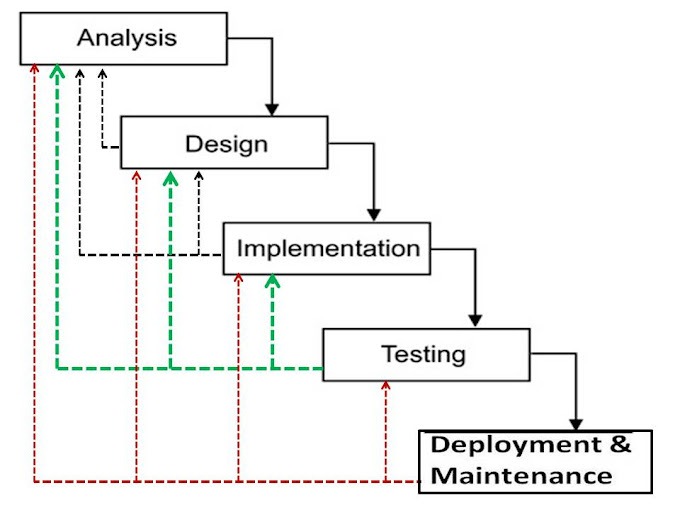
\includegraphics[width=0.6\textwidth]{Images/01 Life_cycle.jpg}  
    \caption{Iterative Waterfall Model}
    \label{Iterative Waterfall Model}  % Label for referencing the figure
\end{figure}


\subsection{Dependencies and Milestones} 
\noindent
Key dependencies were identified for successful project progression. For instance, completion of the data preparation phase was critical before proceeding to model development. Milestones were established at the end of each phase to ensure accountability and track progress. The successful completion of the requirement gathering phase marked the first milestone, followed by the data preparation phase, and so on.

\subsection{Scheduling}
\noindent
Effective scheduling is crucial to the success of any project, as it establishes a clear timeline for tasks, milestones, and dependencies. In the context of our project on detecting mental health disorders through social media analysis, a detailed schedule has been developed to guide the project from inception to completion. This schedule includes specific tasks such as requirement gathering, data preprocessing, model implementation, testing, and deployment, each with clearly defined deadlines. The iterative nature of our chosen methodology allows for flexibility within the schedule, enabling adjustments based on testing outcomes and stakeholder feedback. Key milestones, such as the completion of data analysis, model validation, and user acceptance testing, have been identified to monitor progress and ensure timely delivery of the final product. By utilizing project management tools, such as Microsoft Project, we can visualize and track the progress of tasks, manage resources effectively, and maintain open communication among team members, ensuring that the project stays on schedule and meets its objectives. This proactive approach to scheduling enhances our ability to deliver a high-quality solution that aligns with our goals and stakeholder expectations.

% Insert MS Project Plan Image
\begin{figure}[h!]  
    \centering
    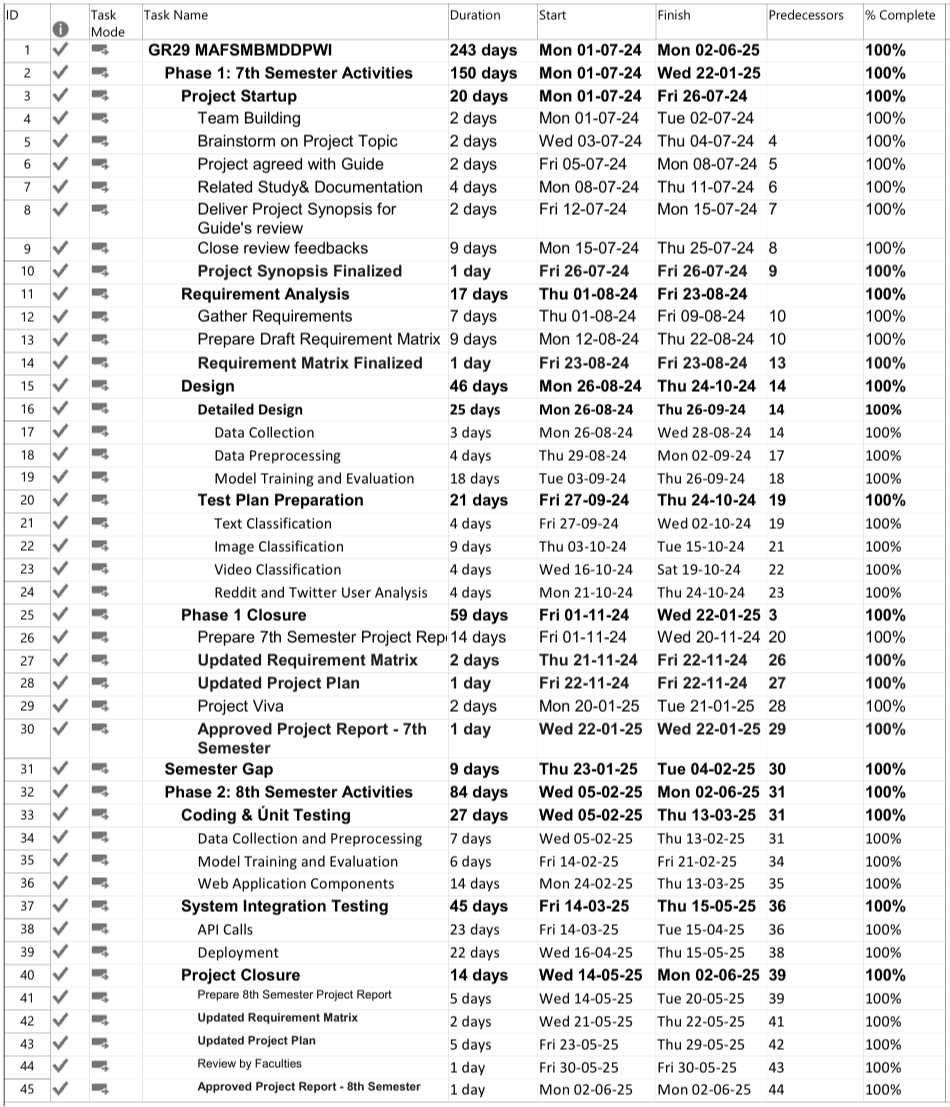
\includegraphics[width=0.9\textwidth]{Images/MS Project Plan Sem 7.png}  
    \caption{Project Plan}
    \label{Project Plan}  % Label for referencing the figure
\end{figure}

\vspace{2cm}

\begin{figure}[h!]  
    \centering
    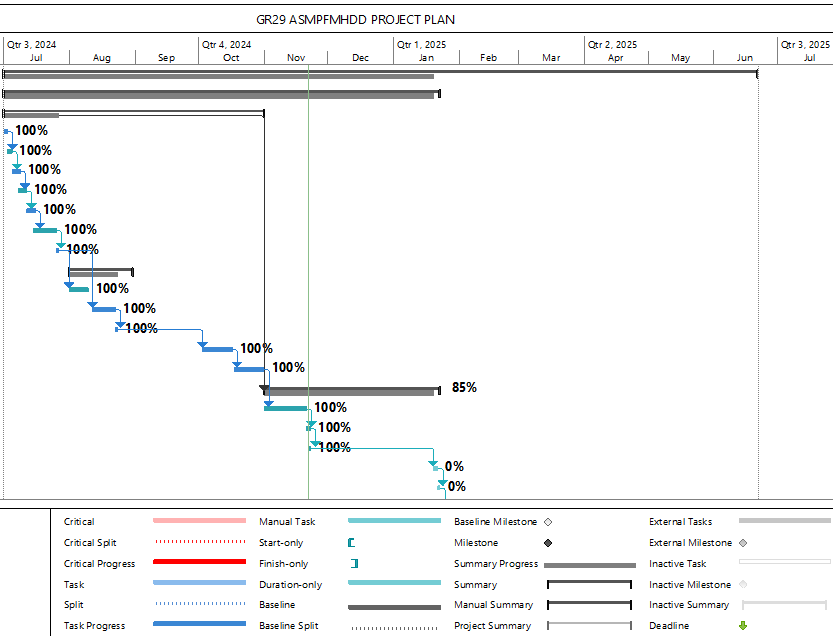
\includegraphics[width=0.9\textwidth]{Images/Gantt Chart.png}  
    \caption{Gantt Chart}
    \label{Gantt Chart}  % Label for referencing the figure
\end{figure}

% ----------------------- Project Planning ends ------------------------------


% --------------------- Requirement Analysis ---------------------------------

\section{Requirement Analysis}

\subsection{Requirement Matrix}
% For Requirement Matrix, latest excel should be pasted and formatted here.
\begin{figure}[h!]  
    \centering
    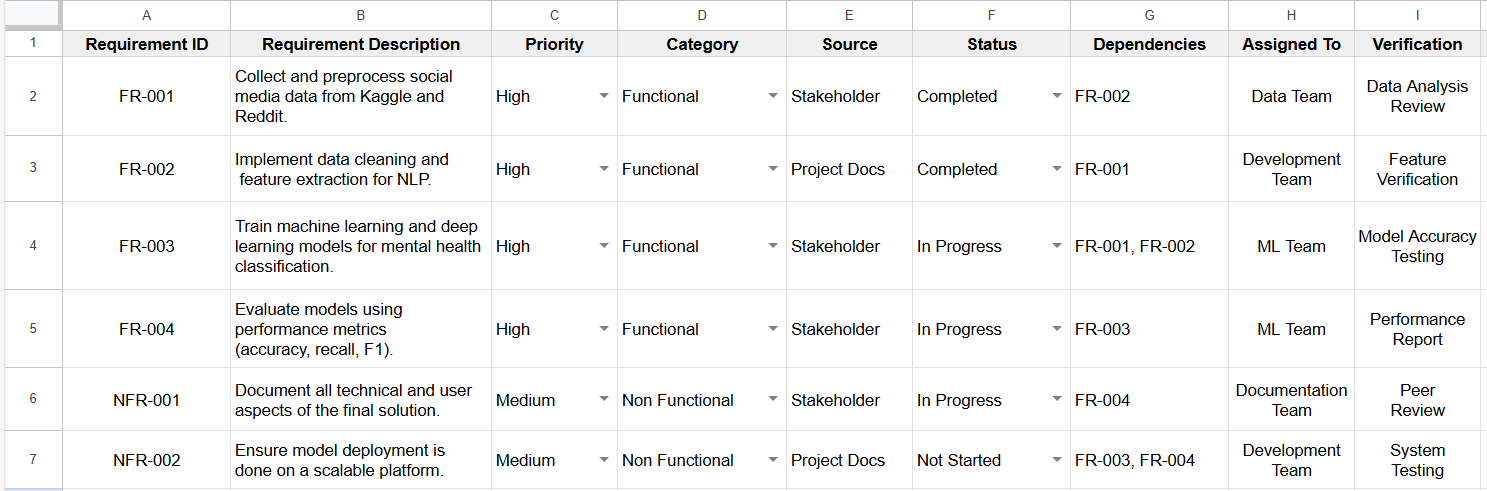
\includegraphics[width=1.0\textwidth]{Images/Requirement Matrix.png}  
    \caption{Requirement Matrix}
    \label{Requirement Matrix}  % Label for referencing the figure
\end{figure}

\noindent
The Requirement Matrix is a comprehensive tool used to track and manage the key requirements of a project. It systematically organizes each requirement with a unique identifier, description, priority, and category (such as functional or non-functional). The matrix also records the source of the requirement, its current status (e.g., in progress, completed), any dependencies on other requirements, and the team or individual responsible for fulfilling it. Additionally, it includes a verification method to ensure the requirement is met, such as through testing or review. This structured format helps ensure that all requirements are clearly defined, prioritized, and tracked, enabling effective project management and ensuring alignment with stakeholder expectations.

\subsection{Requirement Elaboration}
% Create separate sections for separate areas of requirement as in Requirement Matrix. 
% \vspace{.1in}

% \noindent
% For \textbf{Requirement Elaboration}, titles of s6.2.1, 6.2.2 etc. should be with the name of respective requirement areas. Your focus should be on: “What is needed in the system?” Requirement IDs should match with the ID column under Requirement Matrix.

\subsubsection{Functional Requirements}

\noindent
\textbf{\emph{Requirement ID: FR-001}} \\ 
\textbf{\emph{Description: Data Collection}} \\
\textbf{\emph{Priority: High}} \\
\textbf{\emph{Category: Functional}} \\
\noindent
The system requires an ability to collect and ingest a large dataset of Twitter sentiment data from Kaggle. The data should include text content from tweets, associated sentiment labels, and other metadata such as timestamp and user details. This will serve as the primary source of information for sentiment analysis and mental health disorder detection. The system must ensure that the dataset is loaded correctly into the machine learning environment, and any discrepancies in the structure should be handled with pre-processing steps like cleaning, normalization. \\

\noindent
\textbf{\emph{Requirement ID: FR-002}} \\ 
\textbf{\emph{Description: Data Cleaning and Preprocessing}} \\
\textbf{\emph{Priority: High}} \\
\textbf{\emph{Category: Functional}} \\
\noindent
The system must include modules to clean the raw data, such as removing irrelevant characters, handling missing data, and tokenizing text. For the social media posts, it is essential to remove URLs, stopwords, and unnecessary punctuation. The pre-processing pipeline should also convert the text into a suitable numerical format, such as Bag of Words (BoW) or Term Frequency-Inverse Document Frequency (TF-IDF), for further analysis. Proper pre-processing ensures that the data is in a form that can be efficiently used by machine learning models. \\

\noindent
\textbf{\emph{Requirement ID: FR-003}} \\ 
\textbf{\emph{Description: Sentiment and Disorder Detection Model}} \\
\textbf{\emph{Priority: High}} \\
\textbf{\emph{Category: Functional}} \\
\noindent
The system needs to implement machine learning algorithms such as k-Nearest Neighbors (k-NN) and Support Vector Machines (SVM) to classify social media posts based on their sentiment (positive, negative, neutral) and detect potential signs of mental health disorders. The system must be able to train these models on historical data and then apply them to predict the sentiment and detect mental health-related issues in new posts. \\

\noindent
\textbf{\emph{Requirement ID: FR-004}} \\ 
\textbf{\emph{Description: Model Validation and Evaluation}} \\
\textbf{\emph{Priority: High}} \\
\textbf{\emph{Category: Functional}} \\
\noindent
The system must evaluate the performance of the trained models by splitting the dataset into training and test sets. Various performance metrics like accuracy, precision, recall, and F1-score should be computed to assess the model’s effectiveness in detecting mental health disorders. Based on the evaluation, the system should allow for model fine-tuning, such as adjusting hyperparameters, to improve the overall performance. 


\subsubsection{Non Functional Requirements}

\noindent
\textbf{\emph{Requirement ID: NFR-001}} \\ 
\textbf{\emph{Description: Documentation}} \\
\textbf{\emph{Priority: Medium}} \\
\textbf{\emph{Category: Non Functional}} \\
\noindent
The addition of documentation and maintenance manuals as a non-functional requirement ensures that the system is not only usable in the short term but also maintainable and extensible over time. This guarantees that future updates and improvements to the system can be implemented without disrupting existing functionality or requiring a steep learning curve for new developers or users. \\

\noindent
\textbf{\emph{Requirement ID: NFR-002}} \\ 
\textbf{\emph{Description:  Scalability}} \\
\textbf{\emph{Priority: Medium}} \\
\textbf{\emph{Category: Non Functional}} \\
\noindent
The system must be designed to efficiently process large volumes of data, considering the potential growth in the amount of social media posts that need to be analyzed. The data processing pipeline should be scalable to handle increasing data size without significant degradation in performance. This could involve implementing parallel processing techniques or leveraging cloud-based infrastructure to ensure that processing large datasets remains feasible even as the dataset scales. 


% -------------------- Requirement Analysis Ends -----------------------------



% ----------------------------- Design ---------------------------------------

\section{Design}

\subsection{Technical Environment}
% Mention minimum hardware configuration, software tools and package details.
\noindent
The technical environment for the project "Analyzing Social Media Posts for Mental Health Disorder Detection" comprises a combination of hardware, software, and tools that enable smooth data analysis, machine learning model training, and deployment. Below is a detailed overview of the minimum hardware configuration, software tools, and package details necessary to carry out this project effectively. \\

\noindent
\textbf{Minimum Hardware Configuration} \\
\noindent
Given the nature of the project, which involves processing textual data and training machine learning models, the hardware requirements are modest but significant enough to ensure optimal performance. The minimum configuration needed is:
\begin{itemize}
    \item \textbf{Processor} :
    \noindent
    Intel Core i5 (or equivalent) with a base clock speed of at least 2.5 GHz. A multi-core processor is preferred as it helps in parallel processing, which is essential during model training and data preprocessing steps.
    \item \textbf{RAM} :
    \noindent
    8 GB of RAM is recommended to handle the operations of data loading, cleaning, and transformation. Large datasets, like those used in this project, may require more memory to prevent memory overflow errors and reduce delays during processing. For larger datasets, 16 GB of RAM would be ideal.
    \item \textbf{Storage} :
    \noindent
    At least 256 GB of SSD storage is recommended. Faster storage access significantly impacts loading time for datasets and dependencies. SSD is preferred over traditional HDD because of its faster read/write speeds, which benefit large datasets like the Reddit-based social media posts used in this project.
    \item \textbf{Graphics Processing Unit (GPU)} :
    \noindent
    For basic machine learning tasks like Logistic Regression or SVM, a dedicated GPU is not necessary. However, if deep learning models or more complex neural networks were introduced later, a GPU like NVIDIA GTX 1060 with 4 GB VRAM or higher would be advantageous.
    \item \textbf{Operating System} :
    \noindent
    Windows 10 (64-bit) or higher, macOS 10.13 (High Sierra) or higher, or any stable Linux distribution (e.g., Ubuntu 18.04 or higher). The operating system should support all necessary machine learning libraries and be compatible with the tools required for the project.
\end{itemize} \\

\noindent
\textbf{Software Tools and Packages} \\
\noindent
For the software stack, the project leverages a set of well-established tools, platforms, and programming libraries to ensure smooth execution from data preprocessing to model deployment:
\begin{itemize}
    \item \textbf{Python} :
    \noindent
    The primary programming language used for data processing, model training, and evaluation. Python is chosen due to its rich ecosystem of libraries and frameworks tailored for machine learning and data science.
    \item \textbf{Google Colab} :
    \noindent
    A cloud-based platform used for writing, executing, and sharing Python code. Google Colab provides free access to GPU and TPU resources, which is beneficial for intensive model training tasks. It also offers seamless integration with libraries like TensorFlow and PyTorch.
    \item \textbf{Jupyter Notebooks} :
    \noindent
     An alternative environment for running Python code, offering an interactive interface to write and execute code in blocks. It allows for easy visualization of results and is highly suitable for collaborative projects.
\end{itemize}

\pagebreak

\noindent
\textbf{Python Packages and Libraries}
\begin{table}[h!]
\centering
\begin{tabular}{|p{9cm}|p{6cm}|}
  \hline
  \multicolumn{1}{|c|}{\textbf{Package}} & \multicolumn{1}{c|}{\textbf{Purpose}} \\
  
  \hline
  \texttt{praw} & Access Reddit posts for data collection. \\
  
  \hline
  \texttt{pandas} & Data manipulation and analysis. \\
  
  \hline
  \texttt{textblob} & Text processing and sentiment analysis. \\
  
  \hline
  \texttt{time} & Managing execution time. \\
  
  \hline
  \texttt{re} & Regular expressions for text cleaning. \\
  
  \hline
  \texttt{TfidfVectorizer} & Convert text to TF-IDF features. \\
  
  \hline
  \texttt{stopwords} & Remove stopwords from text. \\
  
  \hline
  \texttt{tokenize} & Tokenize text data. \\
  
  \hline
  \texttt{nltk} & Natural Language Toolkit for text processing. \\
  
  \hline
  \texttt{CountVectorizer} & Convert text to Bag-of-Words features. \\
  
  \hline
  \texttt{split} & Split the dataset into training and testing sets. \\
  
  \hline
  \texttt{LogisticRegression} & Build and train Logistic Regression models. \\
  
  \hline
  \texttt{sklearn.metrics.accuracy\_score} & Calculate accuracy of the model. \\
  
  \hline
  \texttt{report} & Generate classification performance report. \\
  
  \hline
  \texttt{RandomizedSearchCV} & Hyperparameter tuning for models. \\
  
  \hline
  \texttt{seaborn} & Data visualization and plotting. \\
  
  \hline
  \texttt{matplotlib.pyplot} & Create and customize plots. \\
  
  \hline
  \texttt{matrix} & Generate confusion matrix. \\
  
  \hline
  \texttt{roc\_curve, auc, roc\_auc\_score} & Evaluate model’s ROC and AUC scores. \\
  
  \hline
  \texttt{KNeighborsClassifier} & Build k-Nearest Neighbors (k-NN) models. \\
  
  \hline
  \texttt{svm.SVC} & Build Support Vector Machines (SVM) models. \\
  
  \hline
  \texttt{naive\_bayes.MultinomialNB} & Build Naive Bayes models. \\
  
  \hline
  \texttt{scipy.stats.uniform} & Statistical operations for tuning models. \\
  
  \hline
  \texttt{RandomForestClassifier} & Build Random Forest models. \\
  
  \hline
  \texttt{sklearn.preprocessing.label\_binarize} & Convert labels for multi-class ROC analysis. \\
  
  \hline
\end{tabular}
\end{table}



\pagebreak

\subsection{Hierarchy of Modules}
% Provide a diagram.
\begin{figure}[h!]  
    \centering
    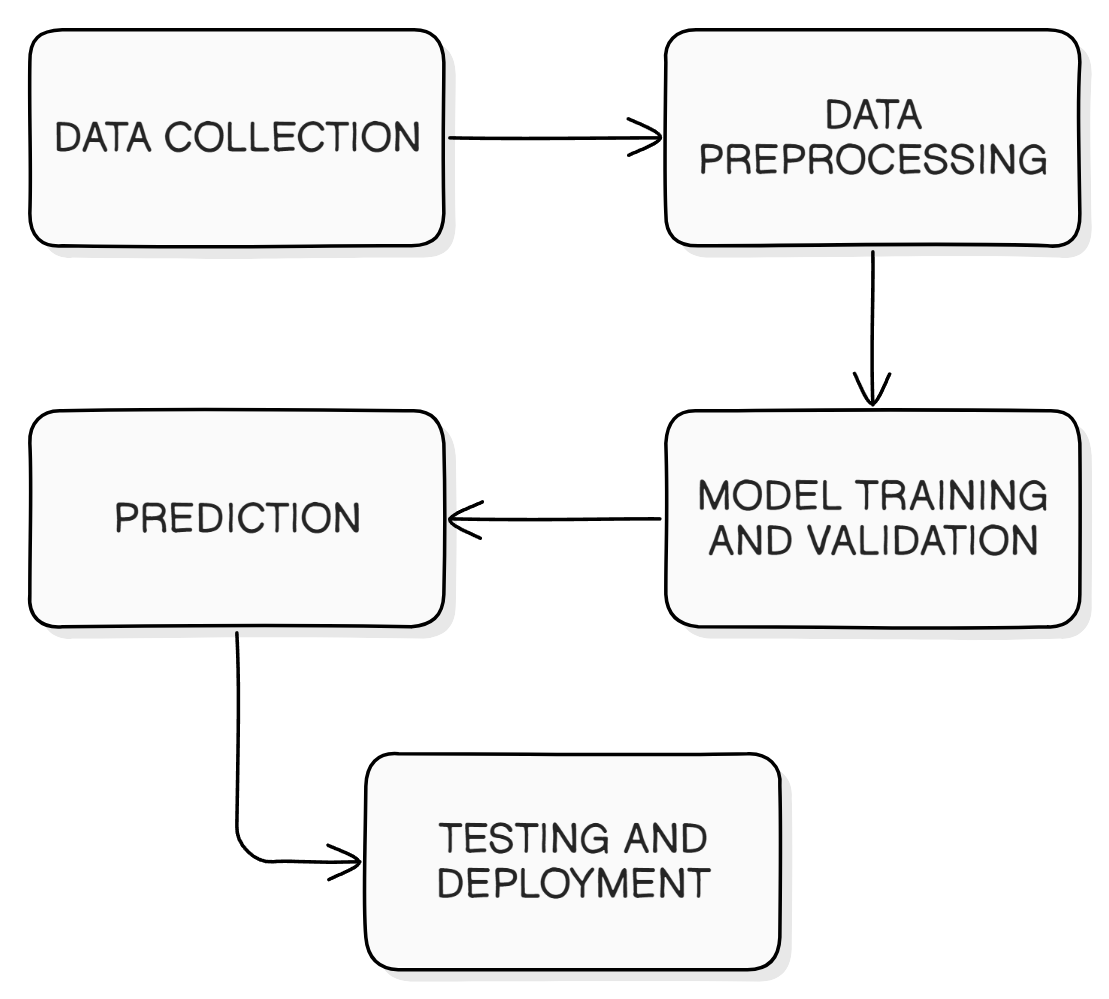
\includegraphics[width=0.6\textwidth]{Images/Project Modules.png}  
    \caption{Project Modules}
    \label{Project Modules}  % Label for referencing the figure
\end{figure}

\noindent
In this project, the system is organized into several key modules to efficiently classify mental health issues based on text input. The Data Loading and Preprocessing Module is responsible for loading the CSV data from preprocessed\_mental\_health\_text.csv and performing essential text cleaning operations, such as tokenization and stop-word removal, to prepare the data for analysis. Following this, the Feature Extraction Module employs techniques like Bag of Words or TF-IDF to convert the cleaned text into numerical features suitable for classification. The Model Training and Validation Module takes these features, splitting the dataset into training and testing sets, and implements multiple machine learning models, including Logistic Regression, k-Nearest Neighbors (k-NN), Support Vector Machines (SVM), Naive Bayes, and Random Forest. Each model is evaluated using relevant metrics to assess accuracy and performance. The Prediction Module is designed to accept new input text and utilize the trained models to predict mental health issues, ensuring that various perspectives from the different algorithms are considered. Finally, the Deployment Module offers a free solution for serving the models, potentially utilizing platforms like Google Colab or Hugging Face, allowing for real-time predictions in practical applications.

\subsection{Detailed Design}
% Provide hierarchy of modules or overall system diagram. 
% \vspace{.1in}
\begin{figure}[h!]  
    \centering
    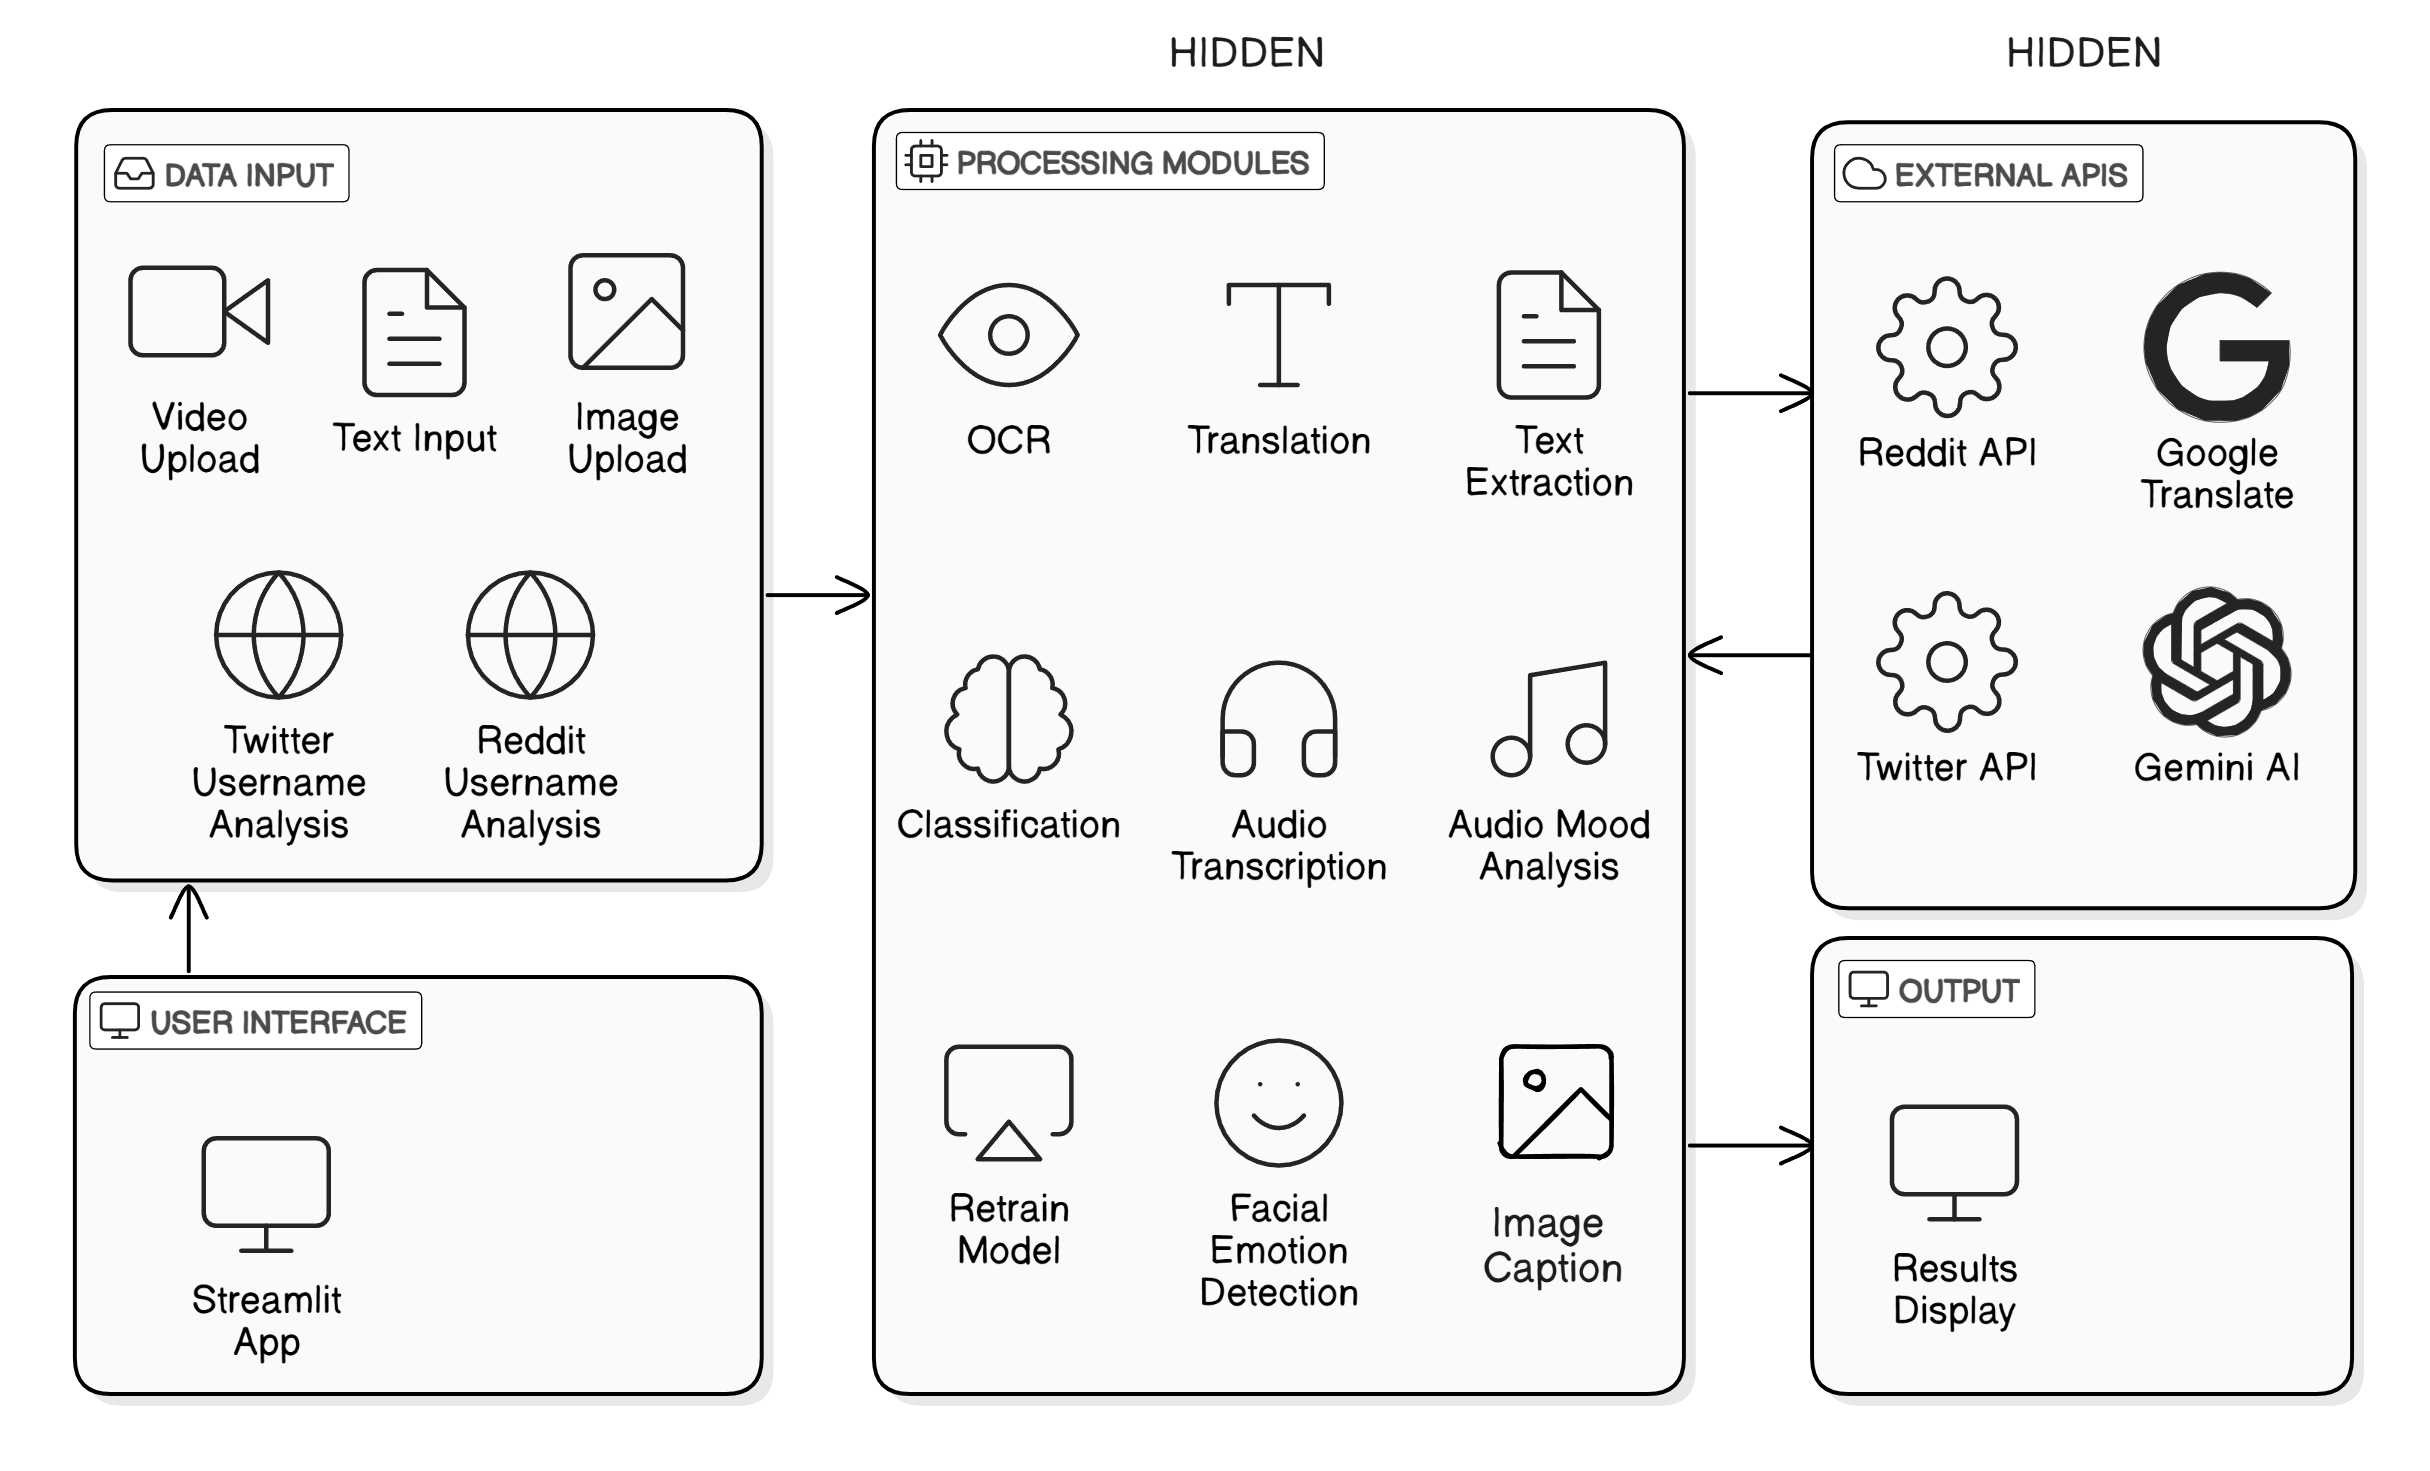
\includegraphics[width=1.0\textwidth]{Images/System Overview.png}  
    \caption{System Overview}
    \label{System Overview}  % Label for referencing the figure
\end{figure}

\begin{figure}[h!]  
    \centering
    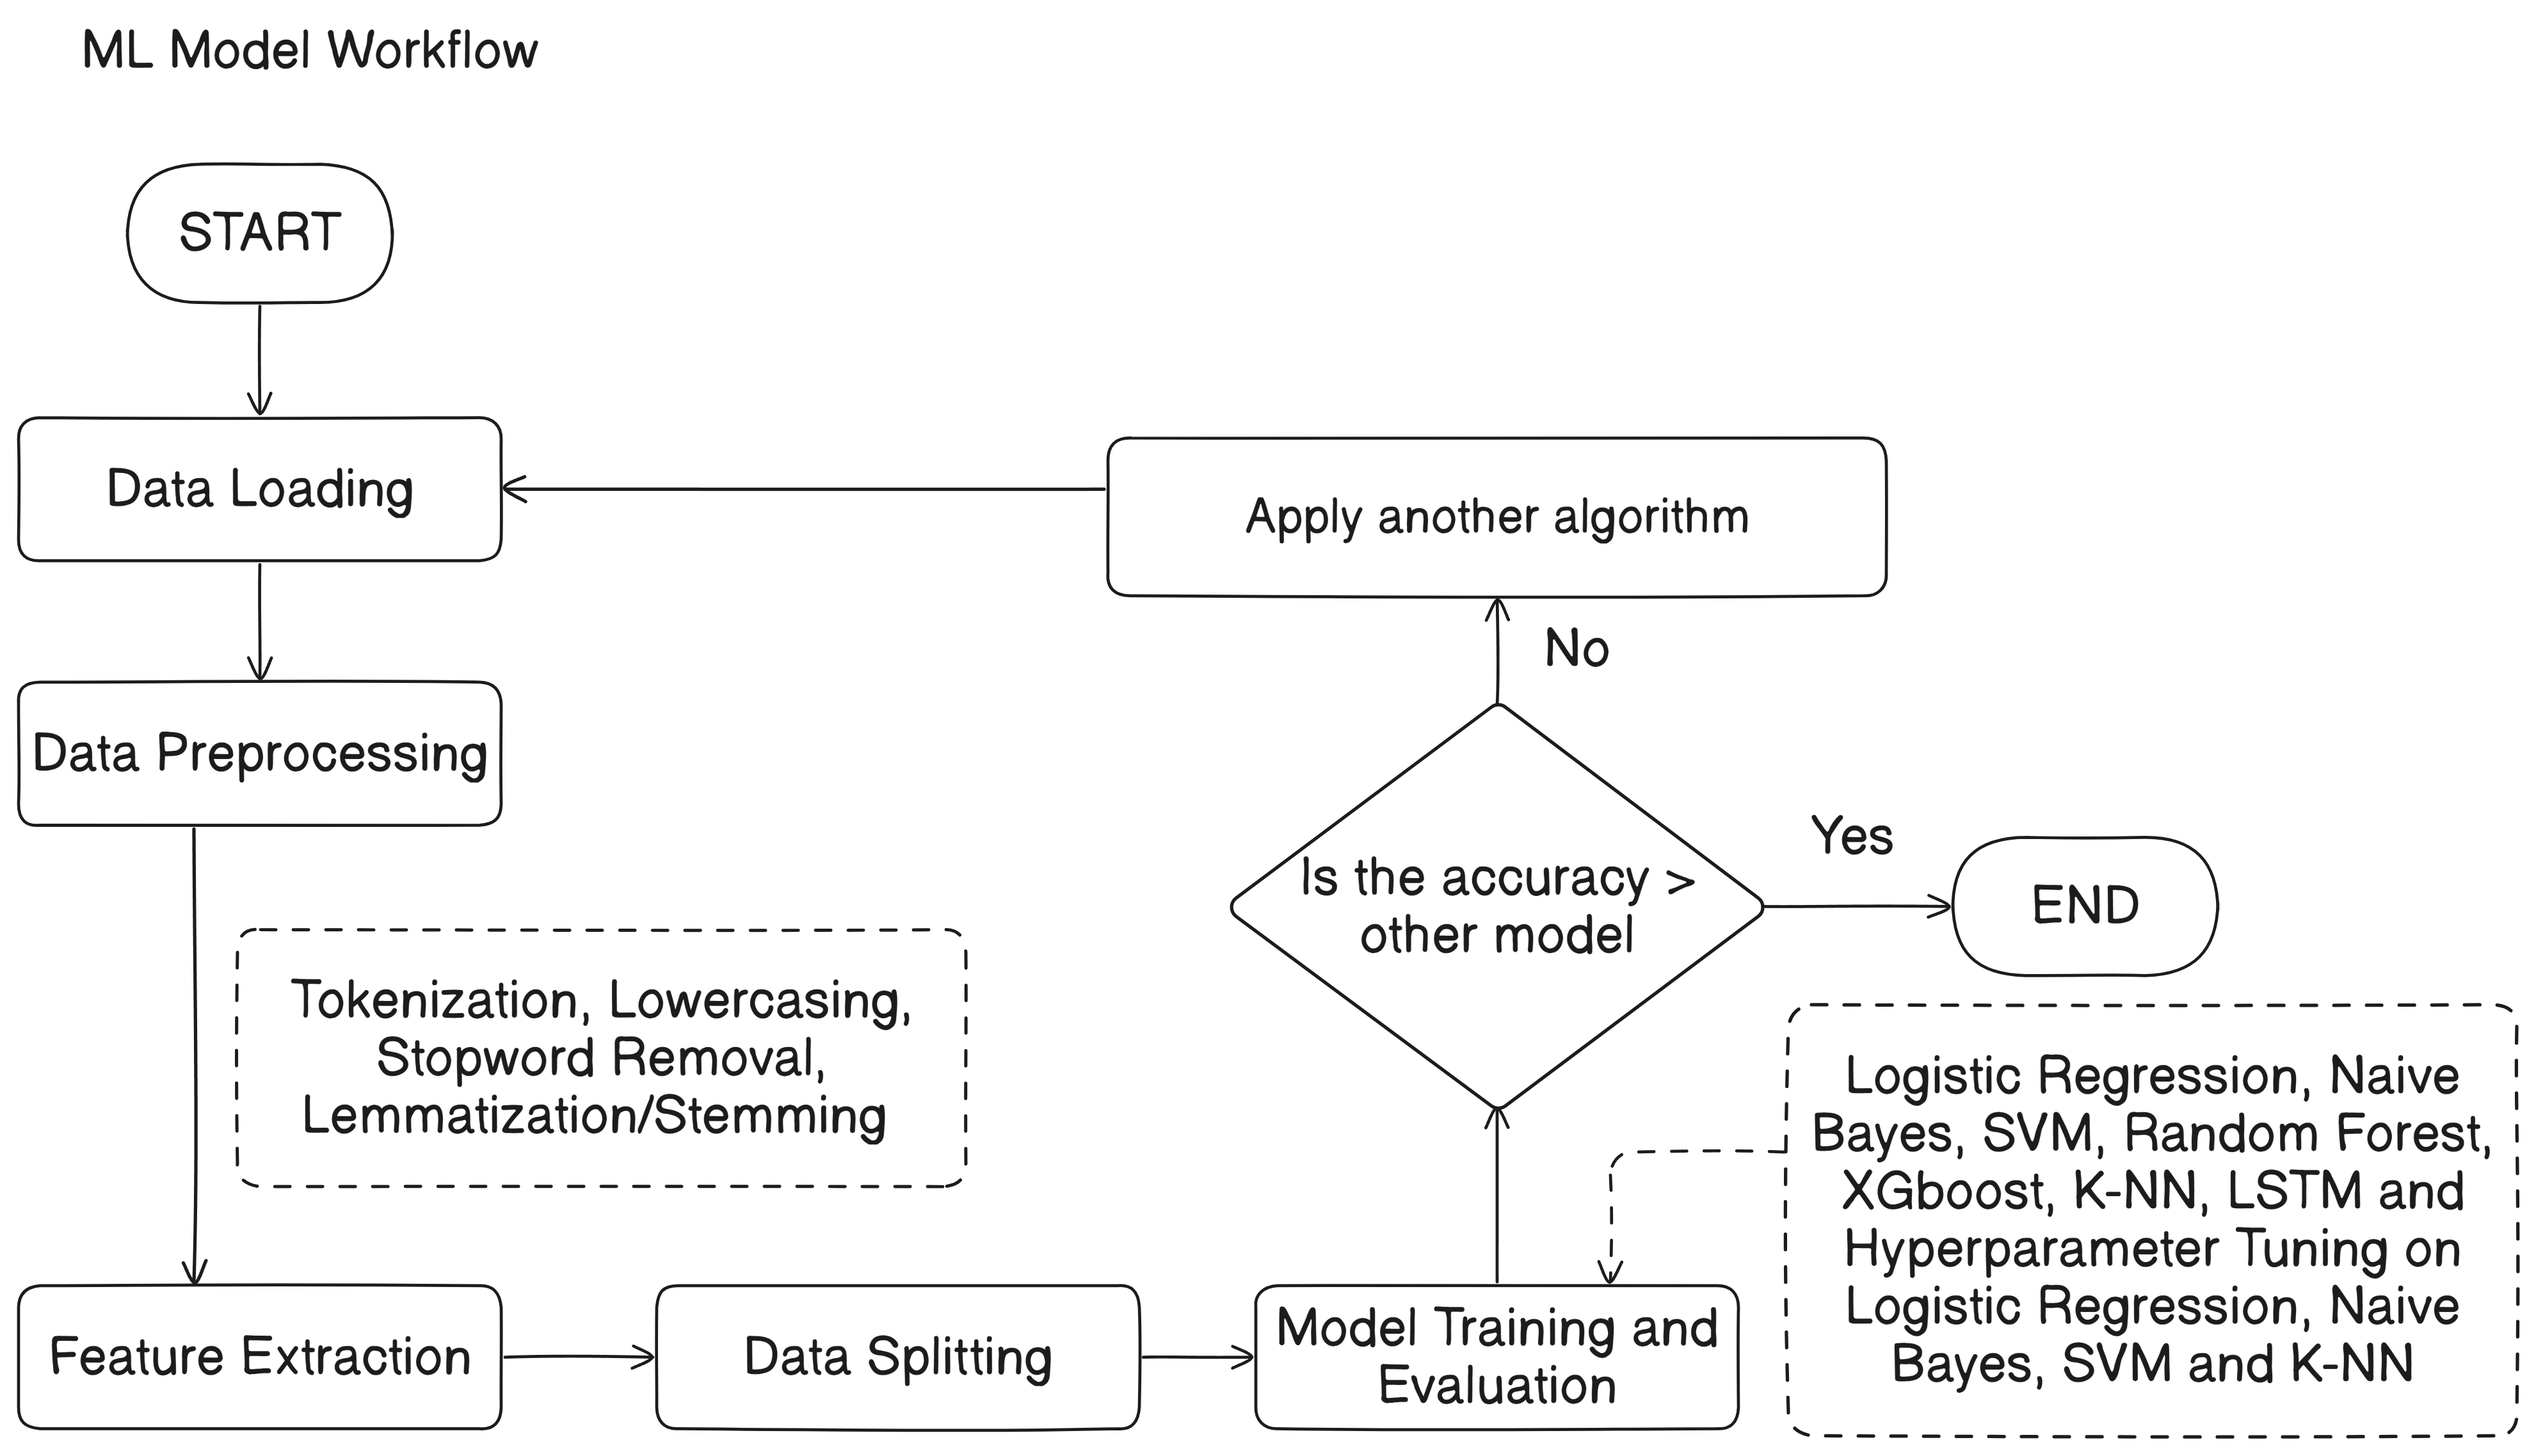
\includegraphics[width=0.95\textwidth]{Images/ML Model Workflow.png}  
    \caption{Model Workflow}
    \label{Model Workflow}  % Label for referencing the figure
\end{figure}

% \noindent
% For Detailed Design, use flowcharts, DFD, UML or ER diagrams as applicable. Titles of s7.2.1, 7.2.2 etc. should be with the name of respective design modules. Your focus should be on: “How the requirement will be implemented in the system?” Design Reference subsection numbers should be matching as stated in Requirement Matrix.
\vspace{.1in}

\subsubsection{Data Loading and Preprocessing}
\noindent
The Data Loading and Preprocessing Module is the foundation of the system, responsible for ingesting and preparing the text data for analysis. This module begins by loading the dataset from the preprocessed\_mental\_health\_text.csv file, which contains various mental health-related text entries. Once the data is loaded, a series of preprocessing steps are conducted to ensure the text is clean and ready for feature extraction. This includes tokenization, where the text is split into individual words or tokens, and lowercasing to maintain uniformity across the dataset. Additionally, stop-word removal is performed to eliminate common words that do not contribute to the meaning, such as "and," "the," and "is." Finally, lemmatization or stemming is applied to reduce words to their base or root forms. These preprocessing techniques are crucial as they help improve the quality of the input data, ultimately leading to better model performance.

\subsubsection{Feature Extraction}
\noindent
In the Feature Extraction Module, the preprocessed text data is transformed into a numerical format that machine learning algorithms can process. This module allows for the selection between two primary feature extraction methods: Bag of Words (BoW) and Term Frequency-Inverse Document Frequency (TF-IDF). The Bag of Words model creates a representation of the text based on the frequency of words, disregarding the order in which they appear, which simplifies the input for classification algorithms. Alternatively, the TF-IDF approach evaluates the importance of words in the dataset by considering their frequency in individual documents relative to their overall occurrence across all documents. This helps in highlighting the most informative words. By converting text into numerical features, this module prepares the data for the subsequent training and validation stages, ensuring that the classification models can effectively interpret the input.

\subsubsection{Model Training and Validation}
\noindent
The Model Training and Validation Module is critical to developing a robust classification system. In this module, the dataset is split into training and testing sets to evaluate the performance of the models accurately. Various classification algorithms are employed, including Logistic Regression, k-Nearest Neighbors (k-NN), Support Vector Machines (SVM), Naive Bayes, and Random Forest. Each model is trained on the training set, which involves adjusting the model parameters based on the input features and their corresponding labels. Following training, the models undergo validation to assess their performance using various metrics such as accuracy, precision, recall, and F1-score. A decision point is included to determine if the achieved accuracy meets the project requirements. If the accuracy is deemed acceptable, the model proceeds to the deployment stage. 

\begin{figure}[h!]  
    \centering
    \includegraphics[width=0.85\textwidth]{Images/Project Sequence.png}  
    \caption{Project Sequence}
    \label{Project Sequence}  % Label for referencing the figure
\end{figure}

\subsubsection{Prediction}
\noindent
The Prediction Module is designed to provide real-time classification of new input text related to mental health issues. Upon receiving user input, this module initiates a preprocessing workflow that mirrors the steps applied during the training phase, including tokenization, lowercasing, stop-word removal, and lemmatization or stemming. Once the input text is preprocessed, it is fed into the trained classification models to generate predictions. Each model may provide a classification result, allowing for a comprehensive analysis of the input. This module not only delivers the predicted mental health issue but also ensures that users receive an informative output that reflects the confidence level of each prediction, enabling them to understand the model's reasoning. The seamless integration of this module into the overall system enhances the user experience by providing instant and relevant feedback.

\subsubsection{Deployment}
\noindent
The Deployment Module focuses on making the trained models accessible for real-time predictions. Once the models have been validated and selected based on their performance, this module prepares them for deployment on suitable platforms, such as Google Colab or Hugging Face. This involves packaging the models and creating a user interface where users can input text and receive predictions. The deployment process also includes considerations for scaling, ensuring that the system can handle multiple requests simultaneously while maintaining responsiveness. By providing a free and efficient deployment solution, this module enables users to access the mental health classification service easily. The deployment of the models ensures that the insights generated from the analysis can be utilized effectively in real-world applications, contributing to better mental health awareness and support.

% \noindent
% Create separate sections for separate modules of design as in Requirement Matrix. Ensure to provide Design Diagrams \textit{(e.g. System overview / DFDs / ERDs etc.; cross-reference to be drawn from Chapter 6), Decision matrix (for algorithm recommendation etc.) }




% \subsubsection{Name of Design Module 1 \label{sec:design_mod1}}
% \subsubsection{Name of Design Module 2 \label{sec:design_mod2}}
% \subsubsection{Name of Design Module 3 etc \label{sec:design_mod3}}


% Refer APPENDIX A  – Prototypes \ref{sec:proto} for prototype details.


% ------------------------------ Design Ends ---------------------------------


% --------------------------- Implementation ---------------------------------

\section{Implementation}
%Focus of 7\textsuperscript{th} semester deliverables are analysis, design and prototyping. Refer APPENDIX A – Prototypes for prototype details.
% For Test Planning, s6.4 should contain the Test Plan in tabular format, where each Test
% Case should be represented with distinct id, prefixed with ``T-$<<$module$>>$-'', where module represents the short code of the respective design module. 
% Test Case numbers should be matching as stated in Requirement Matrix.

\subsection{Features From RM}
\noindent
For the initial prototype development, a subset of the requirements from the Requirement Matrix (RM) was carefully selected to focus on implementing core functionalities and demonstrating proof of concept. The selection was based on a combination of high-priority functional requirements that form the backbone of the system, ensuring that critical features are built and validated before expanding the scope.

The requirements chosen for the prototype primarily involve data preprocessing, model training, and evaluation processes. These requirements were selected because they are fundamental to the project's success, ensuring that the data pipeline and model implementation work seamlessly together. This subset of features lays the groundwork for later integration with additional components and more complex functionality.

The filtered part of the RM focuses on the following high-priority requirements: data cleaning and feature extraction, training of machine learning models, and evaluation of model performance using standard metrics. These requirements were identified as crucial because they directly impact the system's ability to handle data, learn patterns, and provide meaningful outputs. Without successfully implementing these core features, the overall effectiveness of the solution would be significantly reduced.

Furthermore, these selected features align with the project’s goals and provide a clear pathway for incremental development. By narrowing down the requirements to these foundational aspects, the development team can ensure that the prototype is not only functional but also extensible, providing a robust framework for future enhancements.

\begin{figure}[h!]  
    \centering
    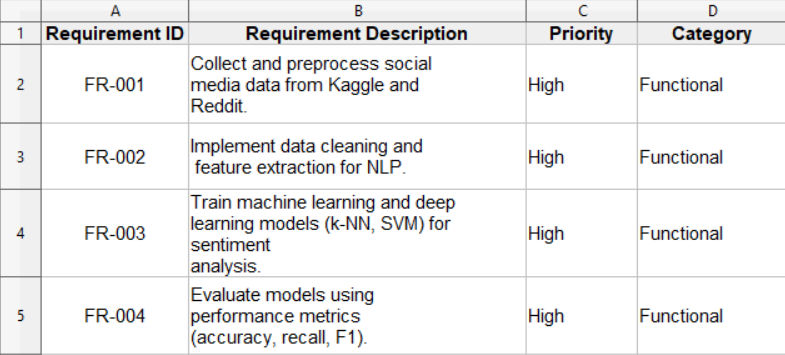
\includegraphics[width=0.85\textwidth]{Images/RM_part_for_implementation.png}  
    \caption{Features from Requirement Matrix}
    \label{Features from Requirement Matrix}  % Label for referencing the figure
\end{figure}

\subsection{Steps of Compilation, Execution and Setup}
\begin{enumerate}
    \item \textbf{Setup the Development Environment}
    \begin{itemize}
        \item Ensure Python 3.x is installed on your system.
        \item Install a virtual environment package if not already available:
        \begin{verbatim}
        pip install virtualenv
        \end{verbatim}
        \item Create a virtual environment for the project:
        \begin{verbatim}
        python -m venv project_env
        \end{verbatim}
        \item Activate the virtual environment:
        \begin{itemize}
            \item For Windows:
            \begin{verbatim}
            .\project_env\Scripts\activate
            \end{verbatim}
            \item For Linux/Mac:
            \begin{verbatim}
            source project_env/bin/activate
            \end{verbatim}
        \end{itemize}
    \end{itemize}

    \item \textbf{Install Required Libraries}
    \begin{itemize}
        \item Install the necessary Python libraries using the following command:
        \begin{verbatim}
        pip install pandas numpy scikit-learn matplotlib
        \end{verbatim}
        \item If your project has additional dependencies, include them as well:
        \begin{verbatim}
        pip install tensorflow keras seaborn
        \end{verbatim}
    \end{itemize}

    \item \textbf{Set Up the Project Directory}
    \begin{itemize}
        \item Organize your project directory as follows:
        \begin{verbatim}
        project_folder/
        ├── data/
        │   └── sample_data.csv
        ├── notebooks/
        │   └── project_prototype.ipynb
        ├── src/
        │   └── main.py
        └── requirements.txt
        \end{verbatim}
        \item Place your input data files in the \texttt{data/} folder.
        \item Store Jupyter notebooks in the \texttt{notebooks/} folder.
        \item Add the main code files in the \texttt{src/} folder.
    \end{itemize}

    \item \textbf{Configure the Jupyter Notebook Environment}
    \begin{itemize}
        \item Navigate to the \texttt{notebooks/} folder using the command line:
        \begin{verbatim}
        cd notebooks
        \end{verbatim}
        \item Launch Jupyter Notebook:
        \begin{verbatim}
        jupyter notebook
        \end{verbatim}
        \item Open the \texttt{project\_prototype.ipynb} file from the Jupyter interface and execute each cell sequentially to run the prototype.
    \end{itemize}

    \item \textbf{Compilation and Execution of the Main Code (If Using Scripts)}
    \begin{itemize}
        \item If you are running the project using a script (e.g., \texttt{main.py}), navigate to the \texttt{src/} folder:
        \begin{verbatim}
        cd ../src
        \end{verbatim}
        \item Run the main script:
        \begin{verbatim}
        python main.py
        \end{verbatim}
        \item Ensure that the paths to the data files and other dependencies are correctly set in your code.
    \end{itemize}

    \item \textbf{Setup Test Data for Evaluation}
    \begin{itemize}
        \item Place the test dataset in the \texttt{data/} folder, ensuring it follows the format specified in the documentation.
        \item If using the command line, you can test with different data files by updating the file path in the code or using command-line arguments.
    \end{itemize}

    \item \textbf{View and Analyze the Output}
    \begin{itemize}
        \item For Jupyter Notebooks, observe the outputs directly in the notebook cells.
        \item If using scripts, the results (e.g., model performance, accuracy metrics, or visualizations) will be printed to the console or saved as files in the \texttt{output/} folder, depending on the implementation.
    \end{itemize}

    \item \textbf{Document and Verify the Execution}
    \begin{itemize}
        \item Document any issues or errors encountered during the compilation and execution.
        \item Perform a verification of results against the expected outputs to ensure correctness.
    \end{itemize}
\end{enumerate}

\subsection{Code Details and Output}

% Data Collection
\subsubsection{Data Collection: Scraping Reddit Posts}
\noindent
The code snippet below demonstrates how Reddit posts related to mental health issues are collected and preprocessed for further analysis. This process involves using the `praw` library to access the Reddit API, collecting posts from specified subreddits, extracting text data, calculating sentiment scores using `TextBlob`, and saving the processed data into a CSV file.

\begin{itemize}
    \item \textbf{Library Installation and Importation:}
    \begin{verbatim}
    !pip install praw
    import praw
    import pandas as pd
    from textblob import TextBlob
    import time
    \end{verbatim}
    \noindent
    The code starts by installing and importing necessary libraries: 
    \texttt{praw} (Python Reddit API Wrapper) for accessing Reddit data, 
    \texttt{pandas} for handling tabular data, 
    \texttt{TextBlob} for sentiment analysis, 
    and \texttt{time} for managing pauses during the scraping process to avoid rate limits.

    \item \textbf{Reddit API Authentication:}
    \begin{verbatim}
    reddit = praw.Reddit(client_id=<Reddit Client ID>,
                         client_secret=<Reddit Client Secret>,
                         user_agent='Mental Health')
    \end{verbatim}
    \noindent
    Here, the Reddit API credentials (`client\_id`, `client\_secret`, and `user\_agent`) are specified to create an authorized `praw.Reddit` object, which will be used to interact with Reddit.

    \item \textbf{Defining Subreddits to Scrape:}
    \begin{verbatim}
    subreddits = ['normal','depression','anxiety','bipolar','ptsd']
    \end{verbatim}
    \noindent
    The subreddits related to mental health are stored in a list named `subreddits`. These communities are targeted for data collection.

    \item \textbf{Setting Up Post Collection:}
    \begin{verbatim}
    post_types = ['hot', 'new', 'top']
    posts_per_type = 1500
    \end{verbatim}
    \noindent
    Three categories of posts are selected: `hot`, `new`, and `top`. The number of posts to be collected from each category is set to 1500.

    \item \textbf{Iterating through Subreddits and Post Types:}
    \begin{verbatim}
    for subreddit in subreddits:
        for post_type in post_types:
            if post_type == 'hot':
                subreddit_posts = reddit.subreddit(subreddit).
                hot(limit=posts_per_type)
            elif post_type == 'new':
                subreddit_posts = reddit.subreddit(subreddit).
                new(limit=posts_per_type)
            elif post_type == 'top':
                subreddit_posts = reddit.subreddit(subreddit).
                top(limit=posts_per_type)
    \end{verbatim}
    \noindent
    Nested loops are used to iterate through each subreddit and post type, creating a collection of posts from each combination.

    \item \textbf{Collecting and Labeling Data:}
    \begin{verbatim}
    for post in subreddit_posts:
        post_content = post.title + " " + post.selftext
        sentiment = TextBlob(post_content).sentiment.polarity
    \end{verbatim}
    \noindent
    Each post’s title and content are concatenated into a single string. Sentiment analysis is then performed using `TextBlob` to generate a polarity score, which ranges from -1 (negative) to 1 (positive).

    \item \textbf{Assigning Sentiment Labels:}
    \begin{verbatim}
    if sentiment > 0:
        sentiment_label = 1.0
    elif sentiment < 0:
        sentiment_label = -1.0
    else:
        sentiment_label = 0.0
    \end{verbatim}
    \noindent
    Based on the polarity score, a label is assigned: 1.0 for positive, -1.0 for negative, and 0.0 for neutral sentiment.

    \item \textbf{Storing Data with Labels:}
    \begin{verbatim}
    issue = subreddit
    data.append([post_content, sentiment_label, issue])
    \end{verbatim}
    \noindent
    Each post is associated with its respective subreddit label (mental health issue type) and stored in the `data` list.

    \item \textbf{Handling Rate Limits:}
    \begin{verbatim}
    time.sleep(2)
    \end{verbatim}
    \noindent
    A two-second delay is introduced after processing each type of post to avoid triggering Reddit’s rate limits.

    \item \textbf{Converting Data to DataFrame and Saving to CSV:}
    \begin{verbatim}
    df = pd.DataFrame(data, columns=['text', 'sentiment', 
    mental_health_issue'])
    df.to_csv('mental_health.csv', index=False)
    \end{verbatim}
    \noindent
    Finally, the collected data is converted into a `pandas` DataFrame with columns for text, sentiment, and mental health issue, and saved to a CSV file named `mental\_health.csv`.
\end{itemize}

% Genrating Final Dataset
\subsubsection{Generating the Final Dataset}

\noindent
The following code snippet combines two separate datasets—`mental\_health.csv` and `twitter\_mh.csv`—into a single CSV file named `mental\_health\_text.csv`. This step is crucial for consolidating different sources of mental health-related data into a unified dataset for further analysis.

\begin{verbatim}
import pandas as pd
\end{verbatim}

\noindent
The \texttt{pandas} library is imported as \texttt{pd}. It is a powerful library for data manipulation and analysis, allowing easy handling of structured data formats such as CSV files.

\begin{verbatim}
# Load the two CSV files
csv1 = pd.read_csv('mental_health.csv')
csv2 = pd.read_csv('twitter_mh.csv')
\end{verbatim}

\noindent
Here, the two CSV files, \texttt{mental\_health.csv} and \texttt{twitter\_mh.csv}, are read into separate \texttt{pandas} DataFrames: \texttt{csv1} and \texttt{csv2}. This operation loads each file into memory for further manipulation.

\begin{verbatim}
# Combine the two dataframes vertically
combined_csv = pd.concat([csv1, csv2], ignore_index=True)
\end{verbatim}

\noindent
The \texttt{pd.concat()} function is used to concatenate the two DataFrames vertically. By setting \texttt{ignore\_index=True}, the function reindexes the rows in the resulting DataFrame, ensuring a continuous index across both files. This approach is used to merge datasets containing similar structures (i.e., same columns).

\begin{verbatim}
# Save the result to a new CSV file
combined_csv.to_csv('mental_health_text.csv', index=False)
\end{verbatim}

\noindent
The combined DataFrame, stored in \texttt{combined\_csv}, is saved as a new CSV file named \texttt{mental\_health\_text.csv}. The parameter \texttt{index=False} ensures that the index column is not included in the output file, resulting in a cleaner dataset.

\begin{verbatim}
print("CSV files combined successfully!")
\end{verbatim}

\noindent
The final line prints a success message: \texttt{"CSV files combined successfully!"}, indicating that the operation completed without errors and the files were merged as intended.


% Data Preprocessing
\subsubsection{Text Preprocessing and Feature Extraction}

\noindent
The following code snippet demonstrates the process of text preprocessing and feature extraction using the Term Frequency-Inverse Document Frequency (TF-IDF) method. This is an essential step in preparing textual data for machine learning models, particularly in natural language processing tasks.

\begin{verbatim}
import pandas as pd
import re
from sklearn.feature_extraction.text import TfidfVectorizer
from nltk.corpus import stopwords
from nltk.tokenize import word_tokenize
import nltk
\end{verbatim}

\noindent
The necessary libraries are imported:
- \texttt{pandas} is imported as \texttt{pd} for data manipulation.
- \texttt{re} is imported for regular expression operations, useful for text cleaning.
- \texttt{TfidfVectorizer} from \texttt{sklearn} is imported for feature extraction.
- \texttt{nltk.corpus.stopwords} and 
- \texttt{nltk.tokenize.word\_tokenize} are imported from the Natural Language Toolkit (NLTK) for text processing.
- The \texttt{nltk} library is imported to access various functionalities.

\begin{verbatim}
# Download stopwords (if you haven't already)
nltk.download('stopwords')
nltk.download('punkt')
\end{verbatim}

\noindent
NLTK’s stopwords and punkt tokenizer resources are downloaded if not previously available. Stopwords are common words (e.g., "and", "the") that are usually removed during text preprocessing, while the punkt tokenizer is necessary for breaking text into words.

\begin{verbatim}
# Load the dataset
df = pd.read_csv('mental_health_text.csv')
\end{verbatim}

\noindent
The dataset, \texttt{mental\_health\_text.csv}, is loaded into a DataFrame named \texttt{df} for further processing.

\begin{verbatim}
# 1. Handling Missing Values
# Remove rows with missing text
df.dropna(subset=['text'], inplace=True)
\end{verbatim}

\noindent
The first preprocessing step handles missing values by removing any rows that contain null values in the \texttt{text} column. The \texttt{dropna()} function is called with \texttt{subset} set to \texttt{text}, and \texttt{inplace=True} ensures that changes are made directly to the original DataFrame.

\begin{verbatim}
# 2. Removing duplicates (if any)
df.drop_duplicates(subset=['text'], inplace=True)
\end{verbatim}

\noindent
Next, any duplicate rows based on the \texttt{text} column are removed using 
the \texttt{drop\_duplicates()} method. This step ensures that each entry in the dataset is unique.


\begin{verbatim}
# 3. Text Preprocessing
# Define a function to clean the text
def clean_text(text):
    # Remove URLs
    text = re.sub(r'http\S+', '', text)
    # Remove mentions (@username)
    text = re.sub(r'@\w+', '', text)
    # Remove special characters, numbers, and punctuations
    text = re.sub(r'[^a-zA-Z\s]', '', text)
    # Convert text to lowercase
    text = text.lower()
    # Tokenize the text
    tokens = word_tokenize(text)
    # Remove stopwords
    tokens = [word for word in tokens if word not in 
    stopwords.words('english')]
    # Join the tokens back into a single string
    clean_text = ' '.join(tokens)
    return clean_text
\end{verbatim}

\noindent
A function named \texttt{clean\_text} is defined to preprocess the text data. The following operations are performed within the function:
- URLs are removed using a regular expression.
- Mentions (usernames starting with @) are stripped out.
- Special characters, numbers, and punctuation are eliminated to retain only alphabetical characters and spaces.
- The text is converted to lowercase to ensure uniformity.
- The \texttt{word\_tokenize} function is applied to split the cleaned text into individual words (tokens).
- Stopwords are removed from the token list.
- Finally, the tokens are rejoined into a single string and returned.

\begin{verbatim}
# Apply the cleaning function to the 'text' column
df['cleaned_text'] = df['text'].apply(clean_text)
\end{verbatim}

\noindent
The \texttt{clean\_text} function is applied to the \texttt{text} column of the DataFrame, and the cleaned text is stored in a new column named \texttt{cleaned\_text}. The \texttt{apply()} method applies the function to each row in the specified column.

\begin{verbatim}
# 4. Feature Extraction using TF-IDF Vectorization
# Initialize the TF-IDF vectorizer
vectorizer = TfidfVectorizer(max_features=5000)  
# You can adjust the max_features
\end{verbatim}

\noindent
The TF-IDF vectorizer is initialized with a maximum feature limit of 5000. This setting ensures that only the top 5000 most important words are considered, which helps in managing the dimensionality of the dataset.

\begin{verbatim}
# Fit and transform the cleaned text data
X = vectorizer.fit_transform(df['cleaned_text'])
\end{verbatim}

\noindent
The \texttt{fit\_transform()} method is called on the cleaned text data, transforming the text into a matrix of TF-IDF features. The result is stored in the variable \texttt{X}.

\begin{verbatim}
# Convert the result to a DataFrame for easier understanding (optional)
X_df = pd.DataFrame(X.toarray(), columns=vectorizer.
get_feature_names_out())
\end{verbatim}

\noindent
The resulting TF-IDF matrix \texttt{X} is converted into a DataFrame, \texttt{X\_df}, with columns named according to the feature names extracted by the vectorizer. This step enhances the readability and usability of the data.

\begin{verbatim}
# You now have a cleaned and vectorized dataset.
print(X_df.head())
\end{verbatim}

\noindent
The first few rows of the cleaned and vectorized dataset are printed to the console, providing a quick overview of the transformed data.

\begin{verbatim}
# Save the preprocessed dataset (optional)
df.to_csv('preprocessed_mental_health_text.csv', index=False)
\end{verbatim}

\noindent
Lastly, the preprocessed DataFrame, which now includes the cleaned text, is saved to a new CSV file named \texttt{preprocessed\_mental\_health\_text.csv}. The parameter \texttt{index=False} ensures that the index column is not included in the output file.

\begin{figure}[h!]  
    \centering
    \includegraphics[width=0.8\textwidth]{Images/Output Data Preprocessing.png}  
    \caption{Data Preprocessing}
    \label{Data Preprocessing}  % Label for referencing the figure
\end{figure}

% Bag Of Words Model
\subsubsection{Implementation of Bag Of Words}

\noindent
The following code snippet implements the Bag of Words (BoW) model for the preprocessed dataset related to mental health. This process converts text data into a numerical format that can be used for machine learning tasks.

\begin{verbatim}
import pandas as pd
from sklearn.feature_extraction.text import CountVectorizer
# Load the preprocessed dataset
dataset = pd.read_csv('preprocessed_mental_health_text.csv')
# Check if 'cleaned_text' column exists
if 'cleaned_text' not in dataset.columns:
    raise ValueError("The dataset must have a 'cleaned_text' column. 
    Ensure text preprocessing has been done.")
# Remove rows with missing values in 'cleaned_text' column
dataset.dropna(subset=['cleaned_text'], inplace=True)
# Initialize the CountVectorizer
vectorizer = CountVectorizer()
# Fit and transform the cleaned text data
X = vectorizer.fit_transform(dataset['cleaned_text'])
# Convert the result to a DataFrame for better visualization (optional)
X_df = pd.DataFrame(X.toarray(), columns=vectorizer.
get_feature_names_out())
# Print the shape of the resulting matrix
print(f'Shape of Bag of Words matrix: {X_df.shape}')
# Print the first few rows of the Bag of Words DataFrame (optional)
print(X_df.head())
\end{verbatim}

\noindent
The code begins by importing the necessary libraries: \texttt{pandas} for data manipulation and \texttt{CountVectorizer} from \texttt{sklearn} for creating the Bag of Words model. It then loads a preprocessed dataset from a CSV file named \texttt{preprocessed\_mental\_health\_text.csv}. A check is performed to ensure that the dataset contains a column labeled \texttt{cleaned\_text}. If this column is absent, a \texttt{ValueError} is raised, prompting the user to ensure text preprocessing is completed. Following this, any rows with missing values in the \texttt{cleaned\_text} column are removed to maintain data integrity. Next, an instance of \texttt{CountVectorizer} is initialized, which will convert the cleaned text into a matrix of token counts. The \texttt{fit\_transform()} method is called on the cleaned text data, generating a sparse matrix \(X\) that represents the Bag of Words model. This matrix is then converted into a DataFrame \texttt{X\_df} for easier visualization, with columns corresponding to the unique words identified in the text. Finally, the shape of the resulting Bag of Words matrix is printed to the console, along with the first few rows of the DataFrame to provide a preview of the transformed data.

\begin{figure}[h!]  
    \centering
    \includegraphics[width=0.8\textwidth]{Images/Output BOW.png}  
    \caption{Implementation of Bag Of Words}
    \label{BOW}  % Label for referencing the figure
\end{figure}

% Splitting DataSet
\subsubsection{Splitting Preprocessed Dataset}
\noindent
The following code snippet demonstrates how to split the preprocessed dataset into training and test sets, which is a crucial step in preparing data for machine learning models.

\begin{verbatim}
import pandas as pd
from sklearn.model_selection import train_test_split

# Load the preprocessed dataset
dataset = pd.read_csv('preprocessed_mental_health_text.csv')

# Check if 'cleaned_text' and 'mental_health_issue' columns exist
if 'cleaned_text' not in dataset.columns or 'mental_health_issue' 
not in dataset.columns:
    raise ValueError("The dataset must have 'cleaned_text' and 
    'mental_health_issue' columns.")

# Remove rows with missing values in 'cleaned_text' column
dataset.dropna(subset=['cleaned_text'], inplace=True) 
#This line has been added

# Initialize the CountVectorizer and fit/transform the cleaned text
from sklearn.feature_extraction.text import CountVectorizer

vectorizer = CountVectorizer()
X = vectorizer.fit_transform(dataset['cleaned_text'])

# Prepare the target variable
y = dataset['mental_health_issue']

# Split the dataset into Training and Test Sets
X_train, X_test, y_train, y_test = train_test_split(X, y, 
test_size=0.2, random_state=42)

# Print the shapes of the resulting datasets
print(f'Shape of X_train: {X_train.shape}')
print(f'Shape of X_test: {X_test.shape}')
print(f'Shape of y_train: {y_train.shape}')
print(f'Shape of y_test: {y_test.shape}')
\end{verbatim}

\noindent
The code begins by importing the necessary libraries, specifically \texttt{pandas} for data manipulation and \texttt{train\_test\_split} from \texttt{sklearn.model\_selection} for splitting the dataset. It then loads 
the preprocessed dataset from a CSV file named \newline
\texttt{preprocessed\_mental\_health\_text.csv}. A validation check is performed to ensure that both the \texttt{cleaned\_text} and 
\texttt{mental\_health\_issue} columns exist in the dataset; if not, a \texttt{ValueError} is raised to alert the user. Next, rows with missing values in the \texttt{cleaned\_text} column are removed to maintain data integrity. After this, the \texttt{CountVectorizer} is initialized to transform the cleaned text into a numerical format suitable for machine learning. The transformed text data is stored in the variable \(X\), while the target variable representing mental health issues is stored in \(y\). The dataset is then split into training and test sets, with 80\% of the data used for training and 20\% for testing, controlled by the \texttt{random\_state} parameter to ensure reproducibility. Finally, the shapes of the resulting training and test datasets are printed to the console, providing insights into the number of samples allocated for training and testing, which is essential for understanding the data distribution.

\begin{figure}[h!]  
    \centering
    \includegraphics[width=0.6\textwidth]{Images/Output Splitting Dataset.png}  
    \caption{Splitting Dataset}
    \label{Splitting Dataset}  % Label for referencing the figure
\end{figure}


\subsubsection{Logistic Regression}
\noindent
The following code snippet demonstrates the training and evaluation of a Logistic Regression model using a preprocessed dataset related to mental health.

\begin{figure}[h!]  
    \centering
    \includegraphics[width=1.0\textwidth]{Images/Logistic Regression.png}  
    \caption{Logistic Regression}
    \label{Logistic Regression}  % Label for referencing the figure
\end{figure}

\begin{verbatim}
import pandas as pd
from sklearn.model_selection import train_test_split
from sklearn.feature_extraction.text import CountVectorizer
from sklearn.linear_model import LogisticRegression
from sklearn.metrics import accuracy_score, classification_report
dataset = pd.read_csv('preprocessed_mental_health_text.csv')
if 'cleaned_text' not in dataset.columns or 'mental_health_issue' 
not in dataset.columns:
    raise ValueError("The dataset must have 'cleaned_text' and 
    'mental_health_issue' columns.")
dataset.dropna(subset=['cleaned_text'], inplace=True)
vectorizer = CountVectorizer()
X = vectorizer.fit_transform(dataset['cleaned_text'])
y = dataset['mental_health_issue']
X_train, X_test, y_train, y_test = train_test_split(X, y, 
test_size=0.2, random_state=42)
model = LogisticRegression(max_iter=2000)
model.fit(X_train, y_train)
y_pred = model.predict(X_test)
accuracy = accuracy_score(y_test, y_pred)
print(f'Accuracy: {accuracy * 100:.2f}%')
print("Classification Report:\n", classification_report(y_test, 
y_pred))
\end{verbatim}

\noindent
The code begins by importing necessary libraries, including \texttt{pandas} for data manipulation and various functions from \texttt{sklearn} for model training and evaluation. It then loads the preprocessed dataset from a CSV file named \texttt{preprocessed\_mental\_health\_text.csv}. A validation check ensures that the dataset contains the required columns, raising an error if either \texttt{cleaned\_text} or \texttt{mental\_health\_issue} is missing. Rows with missing values in the \texttt{cleaned\_text} column are removed to maintain data quality. The \texttt{CountVectorizer} is initialized and used to convert the cleaned text data into a matrix of token counts, stored in \(X\). The target variable, representing mental health issues, is assigned to \(y\). The dataset is then split into training and testing sets, with 80\% used for training and 20\% for testing. A Logistic Regression model is initialized and trained on the training data. Predictions are made on the test set, and the model's accuracy is calculated and printed. Finally, a classification report is generated, providing detailed metrics on the model’s performance across different categories.

\begin{figure}[h!]  
    \centering
    \includegraphics[width=0.8\textwidth]{Images/Output Logistic Regression.png}  
    \caption{Logistic Regression Result}
    \label{Logistic Regression Result}  % Label for referencing the figure
\end{figure}

\subsubsection{Hyperparameter Tuning on Logistic Regression using Random Search}

The following code snippet demonstrates how to perform hyperparameter tuning on a Logistic Regression model using Random Search.

\begin{verbatim}
import pandas as pd
from sklearn.model_selection import train_test_split, 
RandomizedSearchCV
from sklearn.feature_extraction.text import CountVectorizer
from sklearn.linear_model import LogisticRegression
from sklearn.metrics import accuracy_score, classification_report
dataset = pd.read_csv('preprocessed_mental_health_text.csv')
if 'cleaned_text' not in dataset.columns or 'mental_health_issue' 
not in dataset.columns:
    raise ValueError("The dataset must have 'cleaned_text' and 
    'mental_health_issue' columns.")
dataset.dropna(subset=['cleaned_text'], inplace=True)
vectorizer = CountVectorizer()
X = vectorizer.fit_transform(dataset['cleaned_text'])
y = dataset['mental_health_issue']
X_train, X_test, y_train, y_test = train_test_split(X, y, 
test_size=0.2, random_state=42)
model = LogisticRegression(max_iter=200)
param_distributions = {
    'C': [0.001, 0.01, 0.1, 1, 10, 100],
    'penalty': ['l1', 'l2', 'elasticnet', 'none'],
    'solver': ['liblinear', 'saga']
}
random_search = RandomizedSearchCV(estimator=model, 
param_distributions=param_distributions,
n_iter=10, scoring='accuracy', cv=5, n_jobs=-1, random_state=42)
random_search.fit(X_train, y_train)
print("Best Hyperparameters:", random_search.best_params_)
best_model = random_search.best_estimator_
y_pred = best_model.predict(X_test)
accuracy = accuracy_score(y_test, y_pred)
print(f'Accuracy: {accuracy * 100:.2f}%')
print("Classification Report:\n", 
classification_report(y_test, y_pred))
\end{verbatim}

\noindent
The code begins by importing the necessary libraries, including \texttt{pandas} for data manipulation and various functions from \texttt{sklearn} for model training and evaluation. It loads the preprocessed dataset from a CSV file named \newline \texttt{preprocessed\_mental\_health\_text.csv} and checks for the required columns \texttt{cleaned\_text} and \texttt{mental\_health\_issue}. If these columns are not present, a \texttt{ValueError} is raised. The code then removes any rows with missing values in the \texttt{cleaned\_text} column. The \texttt{CountVectorizer} is initialized to convert the cleaned text into a numerical format, which is stored in \(X\), while the target variable representing mental health issues is stored in \(y\). The dataset is split into training and testing sets with 80\% for training and 20\% for testing. A Logistic Regression model is created with a maximum of 200 iterations. The hyperparameter grid for tuning is defined, specifying values for the inverse of regularization strength (\texttt{C}), types of regularization (\texttt{penalty}), and solvers. A \texttt{RandomizedSearchCV} object is initialized to perform the random search over the hyperparameter grid, and the model is fitted using the training data. The best hyperparameters are printed, and the best model is used to make predictions on the test set. Finally, the model's accuracy is calculated and displayed, along with a classification report that provides detailed metrics on the model's performance across different categories.

\begin{figure}[h!]  
    \centering
    \includegraphics[width=0.6\textwidth]{Images/Output HPT LR.png}  
    \caption{Result of Hyperparameter Tuning on Logistic Regression}
    \label{Project Modules}  % Label for referencing the figure
\end{figure}

\begin{figure}[h!]  
    \centering
    \includegraphics[width=0.6\textwidth]{Images/ROC LR.png}  
    \caption{ROC Curve on Logistic Regression}
    \label{ROC LR}  % Label for referencing the figure
\end{figure}


\subsubsection{K Nearest Neighbours}
\noindent
The following code snippet demonstrates the implementation of the k-Nearest Neighbors (k-NN) algorithm for classifying mental health issues based on preprocessed text data.

\begin{figure}[h!]  
    \centering
    \includegraphics[width=1.0\textwidth]{Images/KNN.png}  
    \caption{K Nearest Neighbours Workflow}
    \label{KNN}  % Label for referencing the figure
\end{figure}


\begin{verbatim}
import pandas as pd
from sklearn.model_selection import train_test_split
from sklearn.feature_extraction.text import CountVectorizer
from sklearn.neighbors import KNeighborsClassifier
from sklearn.metrics import accuracy_score, classification_report, 
confusion_matrix
dataset = pd.read_csv('preprocessed_mental_health_text.csv')
if 'cleaned_text' not in dataset.columns or 'mental_health_issue' 
not in dataset.columns:
    raise ValueError("The dataset must have 'cleaned_text' and 
    'mental_health_issue' columns.")
dataset.dropna(subset=['cleaned_text'], inplace=True)
vectorizer = CountVectorizer()
X = vectorizer.fit_transform(dataset['cleaned_text'])
y = dataset['mental_health_issue']
X_train, X_test, y_train, y_test = train_test_split(X, y, 
test_size=0.2, random_state=42)
knn = KNeighborsClassifier(n_neighbors=5)
knn.fit(X_train, y_train)
y_pred = knn.predict(X_test)
accuracy = accuracy_score(y_test, y_pred)
print(f'Accuracy: {accuracy * 100:.2f}%')
print("Classification Report:\n", 
classification_report(y_test, y_pred))
print("Confusion Matrix:\n", confusion_matrix(y_test,y_pred))
\end{verbatim}

\noindent
The code begins by importing the necessary libraries, including \texttt{pandas} for data manipulation, \texttt{train\_test\_split} for splitting the dataset, \texttt{CountVectorizer} for transforming text data, and \texttt{KNeighborsClassifier} along with various metrics from \texttt{sklearn} for model evaluation. It loads the preprocessed dataset from a CSV file named \newline
\texttt{preprocessed\_mental\_health\_text.csv} and checks that both the \texttt{cleaned\_text} and \texttt{mental\_health\_issue} columns are present; if not, a \texttt{ValueError} is raised. Rows with missing values in the \texttt{cleaned\_text} column are removed to maintain data integrity. The \texttt{CountVectorizer} is initialized to convert the cleaned text into a numerical format, stored in \(X\), while the target variable representing mental health issues is assigned to \(y\). The dataset is split into training and testing sets, with 80\% used for training and 20\% for testing. A k-NN classifier is initialized with 5 neighbors, and the model is fitted on the training data. Predictions are made on the test set, and the model's accuracy is calculated and displayed. Finally, a classification report and confusion matrix are printed, providing detailed metrics on the model's performance and insight into its classification results.

\begin{figure}[h!]  
    \centering
    \includegraphics[width=0.6\textwidth]{Images/Output KNN.png}  
    \caption{K Nearest Neighbours Result}
    \label{KNN}  % Label for referencing the figure
\end{figure}

\subsubsection{Hyperparameter Tuning on KNN Using Random Search}
\noindent
The following code snippet demonstrates how to perform hyperparameter tuning on a k-Nearest Neighbors (k-NN) classifier using Random Search to optimize its performance.

\begin{verbatim}
import pandas as pd
from sklearn.model_selection import train_test_split, 
RandomizedSearchCV
from sklearn.feature_extraction.text import CountVectorizer
from sklearn.neighbors import KNeighborsClassifier
from sklearn.metrics import accuracy_score, classification_report, 
confusion_matrix
dataset = pd.read_csv('preprocessed_mental_health_text.csv')
if 'cleaned_text' 
not in dataset.columns or 'mental_health_issue' not in dataset.columns:
    raise ValueError("The dataset must have 'cleaned_text' and 
    'mental_health_issue' columns.")
dataset.dropna(subset=['cleaned_text'], inplace=True)
vectorizer = CountVectorizer()
X = vectorizer.fit_transform(dataset['cleaned_text'])
y = dataset['mental_health_issue']
X_train, X_test, y_train, y_test = train_test_split(X, y, 
test_size=0.2, random_state=42)
knn = KNeighborsClassifier()
param_distributions = {
    'n_neighbors': [3, 4, 5, 6, 7, 8, 9, 10, 11, 12, 13, 
    14, 15, 16, 17, 18, 19, 20],
    'metric': ['euclidean', 'manhattan', 'chebyshev', 'minkowski'],
    'weights': ['uniform', 'distance']
}
random_search = RandomizedSearchCV(estimator=knn, 
param_distributions=param_distributions, 
n_iter=200, scoring='accuracy', cv=5, n_jobs=-1, random_state=42)
random_search.fit(X_train, y_train)
print("Best Hyperparameters:", random_search.best_params_)
best_knn = random_search.best_estimator_
y_pred = best_knn.predict(X_test)
accuracy = accuracy_score(y_test, y_pred)
print(f'Accuracy: {accuracy * 100:.2f}%')
print("Classification Report:\n", 
classification_report(y_test, y_pred))
print("Confusion Matrix:\n", confusion_matrix(y_test, y_pred))
\end{verbatim}

\noindent
The code starts by importing the required libraries, including \texttt{pandas} for data manipulation, and various functions from \texttt{sklearn} for model training, evaluation, and hyperparameter tuning. It loads the preprocessed dataset from a CSV file named \newline \texttt{preprocessed\_mental\_health\_text.csv} and checks for the presence of the necessary columns, raising a \texttt{ValueError} if they are missing. Rows with missing values in the \texttt{cleaned\_text} column are removed to ensure data quality. The \texttt{CountVectorizer} is initialized to convert the cleaned text into a numerical format, stored in \(X\), while the target variable representing mental health issues is assigned to \(y\). The dataset is split into training and testing sets, with 80\% used for training and 20\% for testing. A k-NN classifier is initialized, and a hyperparameter grid is defined, specifying different values for the number of neighbors, distance metrics, and weighting options for the neighbors. The \texttt{RandomizedSearchCV} object is created to perform random search over the hyperparameter grid, and the model is fitted using the training data. After fitting, the best hyperparameters are printed, along with the best k-NN model derived from the search. Predictions are made on the test set, and the accuracy of the model is calculated and displayed. Finally, a classification report and confusion matrix are printed to evaluate the model's performance and provide insights into its classification results.

\begin{figure}[h!]  
    \centering
    \includegraphics[width=0.8\textwidth]{Images/Output KNN.png}  
    \caption{Result of Hyperparameter Tuning on KNN}
    \label{HPT KNN}  % Label for referencing the figure
\end{figure}

\begin{figure}[h!]  
    \centering
    \includegraphics[width=0.8\textwidth]{Images/ROC KNN.png}  
    \caption{ROC curve on KNN}
    \label{ROC KNN}  % Label for referencing the figure
\end{figure}


\subsubsection{Support Vector Machine}
\noindent
The following code snippet demonstrates the implementation of a Support Vector Machine (SVM) classifier for classifying mental health issues based on preprocessed text data.

\begin{figure}[h!]  
    \centering
    \includegraphics[width=0.6\textwidth]{Images/SVM.png}  
    \caption{Support Vector Machine Workflow}
    \label{SVM}  % Label for referencing the figure
\end{figure}

\begin{verbatim}
import pandas as pd
from sklearn.model_selection import train_test_split
from sklearn.feature_extraction.text import CountVectorizer
from sklearn.svm import SVC
from sklearn.metrics import accuracy_score, classification_report, 
confusion_matrix
dataset = pd.read_csv('preprocessed_mental_health_text.csv')
if 'cleaned_text' not in dataset.columns or 'mental_health_issue' 
not in dataset.columns:
    raise ValueError("The dataset must have 'cleaned_text' and 
    'mental_health_issue' columns.")
dataset.dropna(subset=['cleaned_text'], inplace=True)
vectorizer = CountVectorizer()
X = vectorizer.fit_transform(dataset['cleaned_text'])
y = dataset['mental_health_issue']
X_train, X_test, y_train, y_test = train_test_split(X, y, 
test_size=0.2, random_state=42)
svm_model = SVC(kernel='linear', C=1, random_state=42)
svm_model.fit(X_train, y_train)
y_pred = svm_model.predict(X_test)
accuracy = accuracy_score(y_test, y_pred)
print(f'Accuracy: {accuracy * 100:.2f}%')
print("Classification Report:\n", 
classification_report(y_test, y_pred))
print("Confusion Matrix:\n", confusion_matrix(y_test, y_pred))
\end{verbatim}

\noindent
The code begins by importing the necessary libraries, including \texttt{pandas} for data manipulation and various functions from \texttt{sklearn} for model training and evaluation. It loads the preprocessed dataset from a CSV file named \newline \texttt{preprocessed\_mental\_health\_text.csv} and verifies that both the \texttt{cleaned\_text} and \texttt{mental\_health\_issue} columns exist, raising a \texttt{ValueError} if they are missing. Rows with missing values in the \texttt{cleaned\_text} column are removed to maintain data quality. The \texttt{CountVectorizer} is initialized to convert the cleaned text into a numerical format, stored in \(X\), while the target variable representing mental health issues is assigned to \(y\). The dataset is then split into training and testing sets, with 80\% used for training and 20\% for testing. An SVM model is initialized with a linear kernel and a regularization parameter \(C\) set to 1, which can be adjusted based on the specific needs of the analysis. The model is trained using the training data, and predictions are made on the test set. The accuracy of the model is calculated and displayed, along with a classification report and confusion matrix, which provide insights into the model's performance across different categories and the distribution of classification results.

\begin{figure}[h!]  
    \centering
    \includegraphics[width=0.6\textwidth]{Images/Output SVM.png}  
    \caption{Support Vector Machine (Linear Kernel) Result}
    \label{SVM}  % Label for referencing the figure
\end{figure}

\subsubsection{Hyperparameter Tuning on SVM using Random Search}
\noindent
The following code snippet demonstrates how to perform hyperparameter tuning on a Support Vector Machine (SVM) classifier using Random Search to optimize its performance.

\begin{verbatim}
import pandas as pd
from sklearn.model_selection import train_test_split, 
RandomizedSearchCV
from sklearn.feature_extraction.text import CountVectorizer
from sklearn.svm import SVC
from sklearn.metrics import accuracy_score, classification_report
dataset = pd.read_csv('preprocessed_mental_health_text.csv')
if 'cleaned_text' not in dataset.columns or 'mental_health_issue'
not in dataset.columns:
    raise ValueError("The dataset must have 'cleaned_text' and 
    'mental_health_issue' columns.")
dataset.dropna(subset=['cleaned_text'], inplace=True)
vectorizer = CountVectorizer()
X = vectorizer.fit_transform(dataset['cleaned_text'])
y = dataset['mental_health_issue']
X_train, X_test, y_train, y_test = train_test_split(X, y, 
test_size=0.2, random_state=42)
model = SVC()
param_distributions = {
    'C': [0.1, 1, 10, 100],
    'kernel': ['linear', 'rbf', 'poly'],
    'gamma': ['scale', 'auto', 0.1, 1],
}
random_search = RandomizedSearchCV(estimator=model, 
param_distributions=param_distributions, 
n_iter=200, scoring='accuracy', 
cv=5, n_jobs=-1, random_state=42)
random_search.fit(X_train, y_train)
print("Best Hyperparameters:", random_search.best_params_)
best_model = random_search.best_estimator_
y_pred = best_model.predict(X_test)
accuracy = accuracy_score(y_test, y_pred)
print(f'Accuracy: {accuracy * 100:.2f}%')
print("Classification Report:\n", 
classification_report(y_test, y_pred))
\end{verbatim}

\noindent
The code begins by importing the required libraries, including \texttt{pandas} for data manipulation and various functions from \texttt{sklearn} for model training and evaluation. It loads the preprocessed dataset from a CSV file named \newline \texttt{preprocessed\_mental\_health\_text.csv} and checks for the necessary columns, raising a \texttt{ValueError} if either the \texttt{cleaned\_text} or \texttt{mental\_health\_issue} columns are missing. Rows with missing values in the \texttt{cleaned\_text} column are then removed to ensure data quality. The \texttt{CountVectorizer} is initialized to convert the cleaned text into a numerical format, stored in \(X\), while the target variable representing mental health issues is assigned to \(y\). The dataset is split into training and testing sets, with 80\% used for training and 20\% for testing. An SVM model is initialized, and a hyperparameter grid is defined that specifies different values for the regularization parameter \(C\), various kernel types, and kernel coefficients. The \texttt{RandomizedSearchCV} object is created to perform random search over the hyperparameter grid, and the model is fitted using the training data. After fitting, the best hyperparameters are printed along with the best SVM model derived from the search. Predictions are made on the test set, and the accuracy of the model is calculated and displayed, along with a classification report that provides detailed metrics on the model's performance.

\begin{figure}[h!]  
    \centering
    \includegraphics[width=0.8\textwidth]{Images/Output HPT SVM.png}  
    \caption{Result of Hyperparameter Tuning on SVM}
    \label{HPT SVM}  % Label for referencing the figure
\end{figure}

\begin{figure}[h!]  
    \centering
    \includegraphics[width=0.8\textwidth]{Images/ROC SVM.png}  
    \caption{ROC Curve on SVM}
    \label{ROC SVM}  % Label for referencing the figure
\end{figure}

\pagebreak

\subsubsection{Naive Bayes Result}
\noindent
The following code snippet demonstrates the implementation of a Naive Bayes classifier for classifying mental health issues based on preprocessed text data.

\begin{figure}[h!]  
    \centering
    \includegraphics[width=1.0\textwidth]{Images/Naive Bayes.png}  
    \caption{Naive Bayes Workflow}
    \label{Naive Bayes}  % Label for referencing the figure
\end{figure}

\begin{verbatim}
import pandas as pd
from sklearn.model_selection import train_test_split
from sklearn.feature_extraction.text import CountVectorizer
from sklearn.naive_bayes import MultinomialNB
from sklearn.metrics import accuracy_score, classification_report, 
confusion_matrix
dataset = pd.read_csv('preprocessed_mental_health_text.csv')
if 'cleaned_text' not in dataset.columns or 'mental_health_issue' 
not in dataset.columns:
    raise ValueError("The dataset must have 'cleaned_text' and 
    'mental_health_issue' columns.")
dataset.dropna(subset=['cleaned_text'], inplace=True)
vectorizer = CountVectorizer()
X = vectorizer.fit_transform(dataset['cleaned_text'])
y = dataset['mental_health_issue']
X_train, X_test, y_train, y_test = train_test_split(X, y, 
test_size=0.2, random_state=42)
naive_bayes_model = MultinomialNB()
naive_bayes_model.fit(X_train, y_train)
y_pred = naive_bayes_model.predict(X_test)
accuracy = accuracy_score(y_test, y_pred)
print(f'Accuracy: {accuracy * 100:.2f}%')
print("Classification Report:\n", 
classification_report(y_test, y_pred))
print("Confusion Matrix:\n", confusion_matrix(y_test, y_pred))
\end{verbatim}

\noindent
The code begins by importing the necessary libraries, including \texttt{pandas} for data manipulation and various functions from \texttt{sklearn} for model training and evaluation. It loads the preprocessed dataset from a CSV file named \newline
\texttt{preprocessed\_mental\_health\_text.csv} and checks for the required columns, raising a \texttt{ValueError} if either the \texttt{cleaned\_text} or \texttt{mental\_health\_issue} columns are missing. Rows with missing values in the \texttt{cleaned\_text} column are then removed to ensure data quality. The \texttt{CountVectorizer} is initialized to convert the cleaned text into a numerical format, which is stored in \(X\), while the target variable representing mental health issues is assigned to \(y\). The dataset is split into training and testing sets, with 80\% used for training and 20\% for testing. A Naive Bayes classifier, specifically \texttt{MultinomialNB}, is initialized and fitted using the training data. Predictions are made on the test set, and the model's accuracy is calculated and displayed. Finally, a classification report and confusion matrix are printed, providing detailed metrics on the model's performance across different categories and insights into its classification results.

\begin{figure}[h!]  
    \centering
    \includegraphics[width=0.8\textwidth]{Images/Output NB.png}  
    \caption{Naive Bayes}
    \label{NB}  % Label for referencing the figure
\end{figure}

\subsubsection{Hyperparameter Tuning on Naive Bayes using Random Search}
\noindent
The following code snippet demonstrates how to perform hyperparameter tuning on a Naive Bayes classifier using Random Search to optimize its performance.

\begin{verbatim}
import pandas as pd
from sklearn.model_selection import train_test_split, 
RandomizedSearchCV
from sklearn.feature_extraction.text import CountVectorizer
from sklearn.naive_bayes import MultinomialNB
from sklearn.metrics import accuracy_score, classification_report, 
confusion_matrix
from scipy.stats import uniform
dataset = pd.read_csv('preprocessed_mental_health_text.csv')
if 'cleaned_text' not in dataset.columns or 'mental_health_issue' 
not in dataset.columns:
    raise ValueError("The dataset must have 'cleaned_text' and 
    'mental_health_issue' columns.")
dataset.dropna(subset=['cleaned_text'], inplace=True)
vectorizer = CountVectorizer()
X = vectorizer.fit_transform(dataset['cleaned_text'])
y = dataset['mental_health_issue']
X_train, X_test, y_train, y_test = train_test_split(X, y, 
test_size=0.2, random_state=42)
naive_bayes_model = MultinomialNB()
param_distributions = {
    'alpha': uniform(0.001, 5.0)
}
random_search = RandomizedSearchCV(estimator=naive_bayes_model, 
param_distributions=param_distributions, n_iter=2000, 
scoring='accuracy', cv=5, n_jobs=-1, random_state=42)
random_search.fit(X_train, y_train)
print("Best Hyperparameters:", random_search.best_params_)
best_model = random_search.best_estimator_
y_pred = best_model.predict(X_test)
accuracy = accuracy_score(y_test, y_pred)
print(f'Accuracy: {accuracy * 100:.2f}%')
print("Classification Report:\n", 
classification_report(y_test, y_pred))
print("Confusion Matrix:\n", confusion_matrix(y_test, y_pred))
\end{verbatim}

\noindent
The code begins by importing the necessary libraries, including \texttt{pandas} for data manipulation, various functions from \texttt{sklearn} for model training and evaluation, and \texttt{uniform} from \texttt{scipy.stats} for sampling. It loads the preprocessed dataset from a CSV file named \texttt{preprocessed\_mental\_health\_text.csv} and checks for the presence of the required columns, raising a \texttt{ValueError} if either the \texttt{cleaned\_text} or \texttt{mental\_health\_issue} columns are missing. Rows with missing values in the \texttt{cleaned\_text} column are removed to maintain data quality. The \texttt{CountVectorizer} is initialized to convert the cleaned text into a numerical format, which is stored in \(X\), while the target variable representing mental health issues is assigned to \(y\). The dataset is split into training and testing sets, with 80\% used for training and 20\% for testing. A Naive Bayes classifier, specifically \texttt{MultinomialNB}, is initialized, and a parameter distribution is defined for hyperparameter tuning using Random Search. The \texttt{RandomizedSearchCV} object is created to perform random search over the hyperparameter grid, and the model is fitted using the training data. After fitting, the best hyperparameters are printed along with the best Naive Bayes model derived from the search. Predictions are made on the test set, and the accuracy of the model is calculated and displayed, along with a classification report and confusion matrix that provide detailed metrics on the model's performance across different categories.

\begin{figure}[h!]  
    \centering
    \includegraphics[width=0.8\textwidth]{Images/Output HPT NB.png}  
    \caption{Result of Hyperparameter Tuning on Naive Bayes}
    \label{HPT NB}  % Label for referencing the figure
\end{figure}

\begin{figure}[h!]  
    \centering
    \includegraphics[width=0.8\textwidth]{Images/ROC NB.png}  
    \caption{ROC Curve on Naive bayes}
    \label{ROC NB}  % Label for referencing the figure
\end{figure}

\subssubection{Random Forest}
\noindent
The following code snippet demonstrates the implementation of a Random Forest classifier for classifying mental health issues based on preprocessed text data.

\begin{figure}[h!]  
    \centering
    \includegraphics[width=0.6\textwidth]{Images/Random Forest.png}  
    \caption{Random Forest Workflow}
    \label{Random Forest}  % Label for referencing the figure
\end{figure}

\begin{verbatim}
import pandas as pd
from sklearn.model_selection import train_test_split
from sklearn.feature_extraction.text import CountVectorizer
from sklearn.ensemble import RandomForestClassifier
from sklearn.metrics import accuracy_score, classification_report, 
confusion_matrix
dataset = pd.read_csv('preprocessed_mental_health_text.csv')
if 'cleaned_text' not in dataset.columns or 'mental_health_issue' 
not in dataset.columns:
    raise ValueError("The dataset must have 'cleaned_text' and 
    'mental_health_issue' columns.")
dataset.dropna(subset=['cleaned_text'], inplace=True)
vectorizer = CountVectorizer()
X = vectorizer.fit_transform(dataset['cleaned_text'])
y = dataset['mental_health_issue']
X_train, X_test, y_train, y_test = train_test_split(X, y, 
test_size=0.2, random_state=42)
rf_model = RandomForestClassifier(
    n_estimators=3000,
    max_depth=None,
    min_samples_split=20,
    min_samples_leaf=1,
    max_features='sqrt',
    bootstrap=False,
    random_state=42
)
rf_model.fit(X_train, y_train)
y_pred = rf_model.predict(X_test)
accuracy = accuracy_score(y_test, y_pred)
print(f'Accuracy: {accuracy * 100:.2f}%')
print("Classification Report:\n", 
classification_report(y_test, y_pred))
print("Confusion Matrix:\n", confusion_matrix(y_test, y_pred))
\end{verbatim}

\noindent
The code begins by importing the necessary libraries, including \texttt{pandas} for data manipulation and various functions from \texttt{sklearn} for model training and evaluation. It loads the preprocessed dataset from a CSV file named \texttt{preprocessed\_mental\_health\_text.csv} and checks for the presence of the required columns, raising a \texttt{ValueError} if either the \texttt{cleaned\_text} or \texttt{mental\_health\_issue} columns are missing. Rows with missing values in the \texttt{cleaned\_text} column are then removed to ensure data quality. \\

\noindent
The \texttt{CountVectorizer} is initialized to convert the cleaned text into a numerical format, which is stored in \(X\), while the target variable representing mental health issues is assigned to \(y\). The dataset is split into training and testing sets, with 80\% used for training and 20\% for testing. A Random Forest classifier is initialized with specific parameters, including the number of trees (\texttt{n\_estimators}), the minimum number of samples required to split a node (\texttt{min\_samples\_split}), the minimum number of samples in a leaf node (\texttt{min\_samples\_leaf}), and the number of features to consider when looking for the best split (\texttt{max\_features}). The model is then trained using the training data, and predictions are made on the test set. The accuracy of the model is calculated and displayed, along with a classification report and confusion matrix that provide detailed metrics on the model's performance across different categories.

\begin{figure}[h!]  
    \centering
    \includegraphics[width=0.9\textwidth]{Images/Output RF.png}  
    \caption{Random Forest Result}
    \label{Random Forest}  % Label for referencing the figure
\end{figure}

\begin{figure}[h!]  
    \centering
    \includegraphics[width=0.9\textwidth]{Images/ROC RF.png}  
    \caption{ROC Curve on Random Forest}
    \label{ROC RF}  % Label for referencing the figure
\end{figure}



% ------------------------- Implementation Ends -----------------------------


% -------------------- Result and Analysis ----------------------------------

\pagebreak

\section{Results and Analysis}
%Prepare the test plans in tabular format, where each Test Case should be represented with distinct id, prefixed with “$\langle$module$\rangle$ “, where module represents the short code of the respective design module. Test Case numbers should be matching as stated in Requirement Matrix.
%\vspace{.1in}

%\noindent

%Appropriate definition of ‘Performance Metrics’, e.g. Classification Accuracy, Mean Squared Error etc. should be included, as applicable. 
%\vspace{.1in}

%\noindent
%Depending on your specific project, test results can be represented as a table of data with a corresponding pie chart / bar chart as needed. Analysis of test results should be discussed in terms of clear bullet points.

\noindent
The metrics used for evaluating the performance of the classification models include Precision, Recall, F1-Score, and Support, along with the Confusion Matrix. These metrics are crucial for assessing how well the models are able to differentiate between various classes, providing insight into their accuracy, ability to capture relevant instances, and the overall balance between precision and recall. By analyzing these metrics, a comprehensive understanding of the model's performance can be obtained, enabling informed decisions for further optimization and tuning.

\subsection{Classification Metrics and Confusion Matrix}

\begin{itemize}
    \item \textbf{Precision:} Precision is the ratio of correctly predicted positive observations to the total predicted positives. It can be calculated as:
    \[
    \text{Precision} = \frac{TP}{TP + FP}
    \]
    where \( TP \) represents True Positives, and \( FP \) represents False Positives.

    \item \textbf{Recall:} Recall is the ratio of correctly predicted positive observations to all observations in the actual class:
    \[
    \text{Recall} = \frac{TP}{TP + FN}
    \]
    where \( TP \) is True Positives, and \( FN \) is False Negatives.

    \item \textbf{F1-Score:} F1-Score is the harmonic mean of Precision and Recall, calculated as:
    \[
    \text{F1-Score} = 2 \times \frac{\text{Precision} \times \text{Recall}}{\text{Precision} + \text{Recall}}
    \]

    \item \textbf{Support:} Support refers to the number of actual occurrences of each class in the dataset:
    \[
    \text{Support} = \text{Number of samples in the true class}
    \]

    \item \textbf{Confusion Matrix:} A confusion matrix is used to evaluate the performance of a classification model. It is structured as follows:
    \[
    \begin{bmatrix}
    TP & FP \\
    FN & TN
    \end{bmatrix}
    \]
    where:
    \begin{itemize}
        \item \( TP \) = True Positives
        \item \( FP \) = False Positives
        \item \( FN \) = False Negatives
        \item \( TN \) = True Negatives
    \end{itemize}
\end{itemize}

\subsection{Results of Logistic Regression and Hyperparameter Tuning}

\begin{center}
    \caption{Logistic Regression Classification Report (Before Hyperparameter Tuning)} \\
\begin{tabular}{|l|c|c|c|c|}
\hline
\textbf{Class} & \textbf{Precision} & \textbf{Recall} & \textbf{F1-Score} & \textbf{Support} \\ \hline
Anxiety        & 0.78               & 0.73            & 0.75              & 416              \\ \hline
Bipolar        & 0.66               & 0.84            & 0.74              & 412              \\ \hline
Depression     & 0.74               & 0.72            & 0.73              & 443              \\ \hline
Neutral        & 0.08               & 0.06            & 0.07              & 17               \\ \hline
Normal         & 0.78               & 0.22            & 0.34              & 32               \\ \hline
PTSD           & 0.83               & 0.74            & 0.78              & 427              \\ \hline
\textbf{Accuracy} & \multicolumn{4}{|c|}{73.78\%} \\ \hline
\textbf{Macro Avg} & 0.64            & 0.55            & 0.57              & 1747             \\ \hline
\textbf{Weighted Avg} & 0.75         & 0.74            & 0.74              & 1747             \\ \hline
\end{tabular} \\

 \vspace{0.25in}% Reduces space between tables

\caption{Logistic Regression Classification Report (After Hyperparameter Tuning)} \\
\begin{tabular}{|l|c|c|c|c|}
\hline
\textbf{Class} & \textbf{Precision} & \textbf{Recall} & \textbf{F1-Score} & \textbf{Support} \\ \hline
Anxiety        & 0.80               & 0.75            & 0.77              & 416              \\ \hline
Bipolar        & 0.66               & 0.85            & 0.74              & 412              \\ \hline
Depression     & 0.75               & 0.74            & 0.75              & 443              \\ \hline
Neutral        & 0.14               & 0.12            & 0.13              & 17               \\ \hline
Normal         & 0.78               & 0.22            & 0.34              & 32               \\ \hline
PTSD           & 0.86               & 0.75            & 0.80              & 427              \\ \hline
\textbf{Accuracy} & \multicolumn{4}{|c|}{75.27\%} \\ \hline
\textbf{Macro Avg} & 0.67            & 0.57            & 0.59              & 1747             \\ \hline
\textbf{Weighted Avg} & 0.76         & 0.75            & 0.75              & 1747             \\ \hline
\end{tabular} \\

  \vspace{0.25in}% Reduces space between tables

\caption{Confusion Matrix for Logistic Regression (After Hyperparameter Tuning)} \\
\begin{tabular}{|l|c|c|c|c|c|c|}
\hline
\textbf{True Class} & \textbf{Anxiety} & \textbf{Bipolar} & \textbf{Depression} & \textbf{Neutral} & \textbf{Normal} & \textbf{PTSD} \\ \hline
Anxiety             & 310              & 45               & 37                  & 2                & 1               & 21            \\ \hline
Bipolar             & 12               & 349              & 35                  & 5                & 1               & 10            \\ \hline
Depression          & 34               & 62               & 327                 & 2                & 0               & 18            \\ \hline
Neutral             & 1                & 8                & 5                   & 2                & 0               & 1             \\ \hline
Normal              & 1                & 23               & 1                   & 0                & 7               & 0             \\ \hline
PTSD                & 31               & 44               & 29                  & 3                & 0               & 320           \\ \hline
\end{tabular}
\end{center}

\subsection{Explanation of the Results (Logistic Regression)}

\textbf{Overall Performance:}

The Logistic Regression model's initial accuracy was \textbf{73.78\%}, which improved to \textbf{75.27\%} after hyperparameter tuning using Randomized Search.

\textbf{Improvement After Hyperparameter Tuning:}

\begin{itemize}
    \item The tuned model showed a slight increase in accuracy, reflecting an improved ability to distinguish between the different mental health classes.
    \item The precision, recall, and F1-scores for most of the individual classes also showed minor improvements.
\end{itemize}

\textbf{Class-wise Analysis:}

\begin{itemize}
    \item \textbf{Anxiety:} The precision and recall improved slightly, indicating better classification of anxiety-related texts.
    \item \textbf{Bipolar:} A notable increase in recall suggests the tuned model became more sensitive to identifying bipolar instances correctly.
    \item \textbf{Depression:} The performance metrics remained relatively stable, showing the model was consistently able to handle depression cases.
    \item \textbf{Neutral \& Normal:} Low precision and recall values indicate that the model struggles to correctly classify these rare classes, likely due to insufficient support (sample size).
\end{itemize}


\begin{figure}[h!]  
    \centering
    \includegraphics[width=1.0\textwidth]{Images/Confusion Matrix LR.png}  
    \caption{Confusion Matrix for Logistic Regression}
    \label{Project Modules}  % Label for referencing the figure
\end{figure}

\pagebreak
\textbf{Confusion Matrix Analysis:}

\begin{itemize}
    \item The confusion matrix reveals where the model misclassifies different categories. For example:
    \begin{itemize}
        \item \textbf{Anxiety} is often confused with \textbf{Bipolar} and \textbf{Depression}, indicating overlapping features between these classes.
        \item \textbf{PTSD} is more distinct, as shown by a higher number of true positive predictions (320), suggesting that the model can better differentiate this category.
    \end{itemize}
    \item Overall, the confusion matrix helps pinpoint specific classes where the model's predictions are less reliable, providing direction for further improvements.
\end{itemize}




\subsection{Results of K-Nearest Neighbors (KNN) and Hyperparameter Tuning}

\begin{center}
    \caption{KNN Classification Report (Before Hyperparameter Tuning)}
\begin{tabular}{|l|c|c|c|c|}
\hline
\textbf{Class} & \textbf{Precision} & \textbf{Recall} & \textbf{F1-Score} & \textbf{Support} \\ \hline
Anxiety        & 0.60               & 0.36            & 0.45              & 416              \\ \hline
Bipolar        & 0.31               & 0.83            & 0.45              & 412              \\ \hline
Depression     & 0.46               & 0.35            & 0.40              & 443              \\ \hline
Neutral        & 0.00               & 0.00            & 0.00              & 17               \\ \hline
Normal         & 0.29               & 0.06            & 0.10              & 32               \\ \hline
PTSD           & 0.81               & 0.11            & 0.20              & 427              \\ \hline
\textbf{Accuracy} & \multicolumn{4}{|c|}{39.61\%} \\ \hline
\textbf{Macro Avg} & 0.41            & 0.28            & 0.27              & 1747             \\ \hline
\textbf{Weighted Avg} & 0.54         & 0.40            & 0.36              & 1747             \\ \hline
\end{tabular}


\vspace{0.25in}

\caption{Confusion Matrix for KNN (Before Hyperparameter Tuning)}
\begin{tabular}{|l|c|c|c|c|c|c|}
\hline
\textbf{True Class} & \textbf{Anxiety} & \textbf{Bipolar} & \textbf{Depression} & \textbf{Neutral} & \textbf{Normal} & \textbf{PTSD} \\ \hline
Anxiety             & 148              & 221              & 46                  & 0                & 0               & 1             \\ \hline
Bipolar             & 24               & 340              & 42                  & 1                & 3               & 2             \\ \hline
Depression          & 36               & 246              & 154                 & 0                & 0               & 7             \\ \hline
Neutral             & 2                & 14               & 0                   & 0                & 0               & 1             \\ \hline
Normal              & 0                & 30               & 0                   & 0                & 2               & 0             \\ \hline
PTSD                & 38               & 248              & 91                  & 0                & 2               & 48            \\ \hline
\end{tabular}


\vspace{1.5in}

\pagebreak
\caption{KNN Classification Report (After Hyperparameter Tuning)}
\begin{tabular}{|l|c|c|c|c|}
\hline
\textbf{Class} & \textbf{Precision} & \textbf{Recall} & \textbf{F1-Score} & \textbf{Support} \\ \hline
Anxiety        & 0.65               & 0.34            & 0.45              & 416              \\ \hline
Bipolar        & 0.32               & 0.82            & 0.46              & 412              \\ \hline
Depression     & 0.47               & 0.39            & 0.43              & 443              \\ \hline
Neutral        & 0.00               & 0.00            & 0.00              & 17               \\ \hline
Normal         & 0.26               & 0.19            & 0.22              & 32               \\ \hline
PTSD           & 0.73               & 0.15            & 0.24              & 427              \\ \hline
\textbf{Accuracy} & \multicolumn{4}{|c|}{41.27\%} \\ \hline
\textbf{Macro Avg} & 0.40            & 0.31            & 0.30              & 1747             \\ \hline
\textbf{Weighted Avg} & 0.53         & 0.41            & 0.39              & 1747             \\ \hline
\end{tabular}


\vspace{0.25in}

\caption{Confusion Matrix for KNN (After Hyperparameter Tuning)}
\begin{tabular}{|l|c|c|c|c|c|c|}
\hline
\textbf{True Class} & \textbf{Anxiety} & \textbf{Bipolar} & \textbf{Depression} & \textbf{Neutral} & \textbf{Normal} & \textbf{PTSD} \\ \hline
Anxiety             & 143              & 214              & 52                  & 0                & 2               & 5             \\ \hline
Bipolar             & 19               & 337              & 45                  & 1                & 7               & 3             \\ \hline
Depression          & 31               & 223              & 173                 & 1                & 1               & 14            \\ \hline
Neutral             & 0                & 15               & 1                   & 0                & 0               & 1             \\ \hline
Normal              & 0                & 26               & 0                   & 0                & 6               & 0             \\ \hline
PTSD                & 28               & 233              & 97                  & 0                & 7               & 62            \\ \hline
\end{tabular}
\end{center}

\subsection{Explanations for KNN Results}

\begin{itemize}
    \item \textbf{Initial KNN Performance:}
    \begin{itemize}
        \item The initial accuracy of the KNN model is low (\textbf{39.61\%}), indicating that the model struggles to classify the mental health categories effectively.
        \item The recall for the \textbf{Bipolar} class is high (0.83), suggesting that the model is sensitive to detecting bipolar cases but tends to misclassify other categories as bipolar.
        \item Other classes like \textbf{Neutral} and \textbf{Normal} have very low precision and recall, highlighting the model’s inability to distinguish these less frequent categories.
    \end{itemize}

    \item \textbf{After Hyperparameter Tuning:}
    \begin{itemize}
        \item The accuracy improved slightly to \textbf{41.27\%} after tuning with the best hyperparameters \{'weights': 'distance', 'n\_neighbors': 4, 'metric': 'euclidean'\}, indicating minor gains in the classification.
        \item The recall for the \textbf{Anxiety} class decreased, while the precision increased, showing a trade-off in performance.
        \item For the \textbf{Depression} class, both precision and recall increased slightly, indicating that the tuning helped the model distinguish depression cases better.
    \end{itemize}

    \item \textbf{Confusion Matrix Analysis:}
    \begin{itemize}
        \item Many instances of \textbf{Anxiety} and \textbf{Depression} are misclassified as \textbf{Bipolar}, showing overlapping features between these classes.
        \item The class \textbf{PTSD} has a low recall, indicating that most of the PTSD samples are misclassified into other categories.
        \item The class distribution imbalance and similar feature patterns might be contributing to the misclassifications, causing the model to favor more common classes like Bipolar.
    \end{itemize}
\end{itemize}

\begin{figure}[h!]  
    \centering
    \includegraphics[width=1.0\textwidth]{Images/Confusion Matrix KNN.png}  
    \caption{Confusion Matrix for KNN}
    \label{Confusion Matrix KNN}  % Label for referencing the figure
\end{figure}

\pagebreak
\subsection{Results of Support Vector Machine (SVM) and Hyperparameter Tuning}

\begin{center}
    \caption{SVM Classification Report (Before Hyperparameter Tuning)}
\begin{tabular}{|l|c|c|c|c|}
\hline
\textbf{Class} & \textbf{Precision} & \textbf{Recall} & \textbf{F1-Score} & \textbf{Support} \\ \hline
Anxiety        & 0.70               & 0.70            & 0.70              & 416              \\ \hline
Bipolar        & 0.65               & 0.81            & 0.72              & 412              \\ \hline
Depression     & 0.72               & 0.67            & 0.69              & 443              \\ \hline
Neutral        & 0.19               & 0.18            & 0.18              & 17               \\ \hline
Normal         & 0.62               & 0.25            & 0.36              & 32               \\ \hline
PTSD           & 0.81               & 0.71            & 0.76              & 427              \\ \hline
\textbf{Accuracy} & \multicolumn{4}{|c|}{70.75\%} \\ \hline
\textbf{Macro Avg} & 0.61            & 0.55            & 0.57              & 1747             \\ \hline
\textbf{Weighted Avg} & 0.71         & 0.71            & 0.71              & 1747             \\ \hline
\end{tabular}

\vspace{0.25in}

\caption{Confusion Matrix for SVM (Before Hyperparameter Tuning)}
\begin{tabular}{|l|c|c|c|c|c|c|}
\hline
\textbf{True Class} & \textbf{Anxiety} & \textbf{Bipolar} & \textbf{Depression} & \textbf{Neutral} & \textbf{Normal} & \textbf{PTSD} \\ \hline
Anxiety             & 292              & 45               & 44                  & 2                & 1               & 32            \\ \hline
Bipolar             & 23               & 333              & 37                  & 5                & 3               & 11            \\ \hline
Depression          & 59               & 58               & 296                 & 2                & 0               & 28            \\ \hline
Neutral             & 1                & 7                & 5                   & 3                & 0               & 1             \\ \hline
Normal              & 0                & 24               & 0                   & 0                & 8               & 0             \\ \hline
PTSD                & 41               & 47               & 30                  & 4                & 1               & 304           \\ \hline
\end{tabular}

\vspace{0.25in}

\caption{SVM Classification Report (After Hyperparameter Tuning)}
\begin{tabular}{|l|c|c|c|c|}
\hline
\textbf{Class} & \textbf{Precision} & \textbf{Recall} & \textbf{F1-Score} & \textbf{Support} \\ \hline
Anxiety        & 0.78               & 0.71            & 0.74              & 416              \\ \hline
Bipolar        & 0.61               & 0.83            & 0.70              & 412              \\ \hline
Depression     & 0.75               & 0.70            & 0.72              & 443              \\ \hline
Neutral        & 0.13               & 0.12            & 0.12              & 17               \\ \hline
Normal         & 0.57               & 0.12            & 0.21              & 32               \\ \hline
PTSD           & 0.84               & 0.71            & 0.77              & 427              \\ \hline
\textbf{Accuracy} & \multicolumn{4}{|c|}{72.07\%} \\ \hline
\textbf{Macro Avg} & 0.61            & 0.53            & 0.54              & 1747             \\ \hline
\textbf{Weighted Avg} & 0.73         & 0.72            & 0.72              & 1747             \\ \hline
\end{tabular}

\vspace{0.25in}

\caption{Confusion Matrix for SVM (After Hyperparameter Tuning)}
\begin{tabular}{|l|c|c|c|c|c|c|}
\hline
\textbf{True Class} & \textbf{Anxiety} & \textbf{Bipolar} & \textbf{Depression} & \textbf{Neutral} & \textbf{Normal} & \textbf{PTSD} \\ \hline
Anxiety             & 292              & 45               & 44                  & 2                & 1               & 32            \\ \hline
Bipolar             & 23               & 333              & 37                  & 5                & 3               & 11            \\ \hline
Depression          & 59               & 58               & 296                 & 2                & 0               & 28            \\ \hline
Neutral             & 1                & 7                & 5                   & 3                & 0               & 1             \\ \hline
Normal              & 0                & 24               & 0                   & 0                & 8               & 0             \\ \hline
PTSD                & 41               & 47               & 30                  & 4                & 1               & 304           \\ \hline
\end{tabular}
\end{center}

\subsection{Explanations for SVM Results}

\begin{itemize}
    \item \textbf{Initial SVM Performance:}
    \begin{itemize}
        \item The initial accuracy of the SVM model is \textbf{70.75\%}, indicating a moderate performance in classifying mental health categories.
        \item The \textbf{Bipolar} class has a high recall of 0.81, indicating the model's ability to identify most bipolar cases correctly. However, the precision is lower, showing misclassification with other classes.
        \item The \textbf{Neutral} and \textbf{Normal} classes have low precision and recall values, indicating that the model struggles to identify these minority classes.
    \end{itemize}

    \item \textbf{After Hyperparameter Tuning:}
    \begin{itemize}
        \item The accuracy improved slightly to \textbf{72.07\%} with the best hyperparameters \{'kernel': 'linear', 'gamma': 'scale', 'C': 0.1\}.
        \item The recall for the \textbf{Anxiety} and \textbf{Depression} classes increased, indicating better sensitivity to these categories.
        \item The precision for \textbf{PTSD} also improved, suggesting the model has a clearer distinction for this class after tuning.
    \end{itemize}

    \begin{figure}[h!]  
    \centering
    \includegraphics[width=0.8\textwidth]{Images/Confusion Matrix SVM.png}  
    \caption{Confusion Matrix for SVM}
    \label{Confusion Matrix SVM}  % Label for referencing the figure
    \end{figure}

    \item \textbf{Confusion Matrix Analysis:}
    \begin{itemize}
        \item Many instances of \textbf{Anxiety} and \textbf{Depression} are misclassified as \textbf{Bipolar}, showing overlapping features between these classes.
        \item The \textbf{Neutral} and \textbf{Normal} classes have very few true positive predictions, indicating that the SVM model still struggles to capture these less frequent categories.
        \item Overall, the slight improvement in performance after hyperparameter tuning suggests that tuning helped the SVM classifier better balance the trade-offs between precision and recall for most major classes.
    \end{itemize}
\end{itemize}



\subsection{Results of Naive Bayes and Hyperparameter Tuning}

\begin{center}
    \caption{Naive Bayes Classification Report (Before Hyperparameter Tuning)}
\begin{tabular}{|l|c|c|c|c|}
\hline
\textbf{Class} & \textbf{Precision} & \textbf{Recall} & \textbf{F1-Score} & \textbf{Support} \\ \hline
Anxiety        & 0.69               & 0.72            & 0.70              & 416              \\ \hline
Bipolar        & 0.79               & 0.56            & 0.65              & 412              \\ \hline
Depression     & 0.65               & 0.82            & 0.72              & 443              \\ \hline
Neutral        & 0.17               & 0.29            & 0.21              & 17               \\ \hline
Normal         & 0.14               & 0.03            & 0.05              & 32               \\ \hline
PTSD           & 0.73               & 0.72            & 0.72              & 427              \\ \hline
\textbf{Accuracy} & \multicolumn{4}{|c|}{68.92\%} \\ \hline
\textbf{Macro Avg} & 0.53            & 0.52            & 0.51              & 1747             \\ \hline
\textbf{Weighted Avg} & 0.70         & 0.69            & 0.68              & 1747             \\ \hline
\end{tabular}

\vspace{0.25in}

\caption{Confusion Matrix for Naive Bayes (Before Hyperparameter Tuning)}
\begin{tabular}{|l|c|c|c|c|c|c|}
\hline
\textbf{True Class} & \textbf{Anxiety} & \textbf{Bipolar} & \textbf{Depression} & \textbf{Neutral} & \textbf{Normal} & \textbf{PTSD} \\ \hline
Anxiety             & 300              & 14               & 61                  & 8                & 3               & 30            \\ \hline
Bipolar             & 51               & 229              & 78                  & 5                & 0               & 49            \\ \hline
Depression          & 27               & 20               & 362                 & 5                & 1               & 28            \\ \hline
Neutral             & 1                & 6                & 4                   & 5                & 1               & 0             \\ \hline
Normal              & 12               & 2                & 9                   & 1                & 1               & 7             \\ \hline
PTSD                & 46               & 20               & 47                  & 6                & 1               & 307           \\ \hline
\end{tabular}

\vspace{0.25in}

\caption{Naive Bayes Classification Report (After Hyperparameter Tuning)}
\begin{tabular}{|l|c|c|c|c|}
\hline
\textbf{Class} & \textbf{Precision} & \textbf{Recall} & \textbf{F1-Score} & \textbf{Support} \\ \hline
Anxiety        & 0.68               & 0.74            & 0.71              & 277              \\ \hline
Bipolar        & 0.77               & 0.63            & 0.69              & 289              \\ \hline
Depression     & 0.69               & 0.81            & 0.74              & 316              \\ \hline
Neutral        & 0.20               & 0.43            & 0.27              & 14               \\ \hline
Normal         & 0.17               & 0.04            & 0.07              & 23               \\ \hline
PTSD           & 0.75               & 0.69            & 0.72              & 304              \\ \hline
\textbf{Accuracy} & \multicolumn{4}{|c|}{70.16\%} \\ \hline
\textbf{Macro Avg} & 0.54            & 0.56            & 0.53              & 1223             \\ \hline
\textbf{Weighted Avg} & 0.71         & 0.70            & 0.70              & 1223             \\ \hline
\end{tabular}

\vspace{0.25in}

\caption{Confusion Matrix for Naive Bayes (After Hyperparameter Tuning)}
\begin{tabular}{|l|c|c|c|c|c|c|}
\hline
\textbf{True Class} & \textbf{Anxiety} & \textbf{Bipolar} & \textbf{Depression} & \textbf{Neutral} & \textbf{Normal} & \textbf{PTSD} \\ \hline
Anxiety             & 300              & 14               & 61                  & 8                & 3               & 30            \\ \hline
Bipolar             & 51               & 229              & 78                  & 5                & 0               & 49            \\ \hline
Depression          & 27               & 20               & 362                 & 5                & 1               & 28            \\ \hline
Neutral             & 1                & 6                & 4                   & 5                & 1               & 0             \\ \hline
Normal              & 12               & 2                & 9                   & 1                & 1               & 7             \\ \hline
PTSD                & 46               & 20               & 47                  & 6                & 1               & 307           \\ \hline
\end{tabular}    
\end{center}

\subsection{Explanations for Naive Bayes Results}

\begin{itemize}
    \item \textbf{Initial Naive Bayes Performance:}
    \begin{itemize}
        \item The initial accuracy of the Naive Bayes model is \textbf{68.92\%}, indicating moderate classification performance.
        \item The \textbf{Anxiety} and \textbf{Depression} classes have relatively higher recall values, suggesting that the model is sensitive to identifying these categories correctly.
        \item The \textbf{Neutral} and \textbf{Normal} classes have very low precision and recall, indicating that the model struggles to classify these minority classes.
    \end{itemize}

    \item \textbf{After Hyperparameter Tuning:}
    \begin{itemize}
        \item The accuracy increased slightly to \textbf{70.16\%} with the best hyperparameters \{'fit\_prior': True, 'alpha': 0.5\}, showing a minor performance improvement.
        \item The recall for the \textbf{Anxiety} and \textbf{Depression} classes increased, indicating better sensitivity and improved classification for these classes.
        \item However, the precision for the \textbf{Bipolar} class decreased slightly, suggesting a trade-off in correctly identifying true positive cases for this class.
    \end{itemize}
    
    \item \textbf{Confusion Matrix Analysis:}
    \begin{itemize}
        \item Many instances of \textbf{Anxiety} and \textbf{Depression} are misclassified as \textbf{Bipolar}, indicating overlapping feature characteristics between these categories.
        \item The \textbf{Neutral} and \textbf{Normal} classes continue to have very few true positive predictions, highlighting the model’s struggle to capture these less frequent categories.
        \item The increase in recall for major classes like \textbf{Anxiety} and \textbf{Depression} after tuning suggests that the model learned better class-specific distributions.
    \end{itemize}
\end{itemize}

 \begin{figure}[h!]  
    \centering
    \includegraphics[width=0.8\textwidth]{Images/Confusion Matrix NB.png}  
    \caption{Confusion Matrix for Naive Bayes}
    \label{Confusion Matrix NB}  % Label for referencing the figure
    \end{figure}

\subsection{Results of Random Forest and Hyperparameter Tuning}

\begin{center}
    \caption{Random Forest Classification Report}
\begin{tabular}{|l|c|c|c|c|}
\hline
\textbf{Class} & \textbf{Precision} & \textbf{Recall} & \textbf{F1-Score} & \textbf{Support} \\ \hline
Anxiety        & 0.76               & 0.77            & 0.76              & 416              \\ \hline
Bipolar        & 0.70               & 0.77            & 0.74              & 412              \\ \hline
Depression     & 0.69               & 0.80            & 0.74              & 443              \\ \hline
Neutral        & 0.20               & 0.06            & 0.09              & 17               \\ \hline
Normal         & 0.83               & 0.16            & 0.26              & 32               \\ \hline
PTSD           & 0.88               & 0.73            & 0.80              & 427              \\ \hline
\textbf{Accuracy} & \multicolumn{4}{|c|}{74.87\%} \\ \hline
\textbf{Macro Avg} & 0.68            & 0.55            & 0.57              & 1747             \\ \hline
\textbf{Weighted Avg} & 0.75         & 0.75            & 0.74              & 1747             \\ \hline
\end{tabular}

\vspace{0.25in}

\caption{Confusion Matrix for Random Forest}
\begin{tabular}{|l|c|c|c|c|c|c|}
\hline
\textbf{True Class} & \textbf{Anxiety} & \textbf{Bipolar} & \textbf{Depression} & \textbf{Neutral} & \textbf{Normal} & \textbf{PTSD} \\ \hline
Anxiety             & 319              & 38               & 50                  & 0                & 0               & 9             \\ \hline
Bipolar             & 23               & 319              & 53                  & 2                & 1               & 14            \\ \hline
Depression          & 31               & 41               & 353                 & 0                & 0               & 18            \\ \hline
Neutral             & 1                & 9                & 5                   & 1                & 0               & 1             \\ \hline
Normal              & 3                & 24               & 0                   & 0                & 5               & 0             \\ \hline
PTSD                & 43               & 22               & 49                  & 2                & 0               & 311           \\ \hline
\end{tabular}    
\end{center}

\subsection{Explanations for Random Forest Results}

\begin{itemize}
    \item \textbf{Overall Performance:}
    \begin{itemize}
        \item The accuracy of the Random Forest model is \textbf{74.87\%}, indicating a good level of performance in classifying the different mental health categories.
        \item The \textbf{PTSD} class shows the highest precision (0.88) and recall (0.73), suggesting that the model is effective at identifying PTSD cases correctly.
    \end{itemize}

    \item \textbf{Class-wise Analysis:}
    \begin{itemize}
        \item The precision and recall for the \textbf{Anxiety} and \textbf{Depression} classes are reasonably balanced, indicating that the model is adept at classifying these categories.
        \item The \textbf{Bipolar} class has a slightly lower precision but high recall, suggesting that while the model can identify bipolar instances effectively, it also misclassifies some non-bipolar cases as bipolar.
        \item The performance for the \textbf{Neutral} and \textbf{Normal} classes is concerning, with very low recall and F1-scores, indicating that these classes are often misclassified.
    \end{itemize}

    \begin{figure}[h!]  
    \centering
    \includegraphics[width=0.9\textwidth]{Images/Confusion Matrix RF.png}  
    \caption{Confusion Matrix for Random Forest}
    \label{Confusion Matrix RF}  % Label for referencing the figure
    \end{figure}

    \item \textbf{Confusion Matrix Analysis:}
    \begin{itemize}
        \item The confusion matrix reveals that many instances of \textbf{Anxiety} and \textbf{Depression} are correctly classified, with a significant number of \textbf{Neutral} instances being misclassified.
        \item The low count for \textbf{Normal} indicates that the model has trouble distinguishing this category, as evidenced by the high number of false positives.
        \item The high number of true positive predictions for \textbf{PTSD} (311) suggests that the Random Forest model is effective in distinguishing PTSD from other classes, likely due to its ability to handle complex feature interactions well.
    \end{itemize}
\end{itemize}

\subsection{Comparison of Different Models}

\begin{center}
    \centering
    \caption{Datasets Overview} \\
    \vspace{0.05in}
    \begin{tabular}{|l|c|c|c|}
    \hline
    \textbf{Dataset} & \textbf{Capacity} & \textbf{Modality} \\ \hline
    Dataset - Reddit  & 12000              & Single            \\ \hline
    Dataset - Twitter  & 900                & Single            \\ \hline
    DS - Reddit + Twitter & 12900          & Single            \\ \hline
    \end{tabular}

    \vspace{0.25in}

\centering
\caption{Comparison of Classification Metrics for Anxiety}
\begin{tabular}{|l|c|c|c|c|}
\hline
\textbf{Model} & \textbf{Precision} & \textbf{Recall} & \textbf{F1-Score} & \textbf{Support} \\ \hline
Logistic Regression & 0.78 & 0.73 & 0.75 & 416 \\ \hline
KNN                & 0.60 & 0.36 & 0.45 & 416 \\ \hline
SVM                & 0.70 & 0.70 & 0.70 & 416 \\ \hline
Naive Bayes        & 0.69 & 0.72 & 0.70 & 416 \\ \hline
Random Forest      & 0.76 & 0.77 & 0.76 & 416 \\ \hline
\end{tabular}

\vspace{0.25in}

\centering
\caption{Comparison of Classification Metrics for Bipolar}
\begin{tabular}{|l|c|c|c|c|}
\hline
\textbf{Model} & \textbf{Precision} & \textbf{Recall} & \textbf{F1-Score} & \textbf{Support} \\ \hline
Logistic Regression & 0.66 & 0.84 & 0.74 & 412 \\ \hline
KNN                & 0.31 & 0.83 & 0.45 & 412 \\ \hline
SVM                & 0.65 & 0.81 & 0.72 & 412 \\ \hline
Naive Bayes        & 0.79 & 0.56 & 0.65 & 412 \\ \hline
Random Forest      & 0.70 & 0.77 & 0.74 & 412 \\ \hline
\end{tabular}

\vspace{0.25in}

\centering
\caption{Comparison of Classification Metrics for Depression}
\begin{tabular}{|l|c|c|c|c|}
\hline
\textbf{Model} & \textbf{Precision} & \textbf{Recall} & \textbf{F1-Score} & \textbf{Support} \\ \hline
Logistic Regression & 0.74 & 0.72 & 0.73 & 443 \\ \hline
KNN                & 0.46 & 0.35 & 0.40 & 443 \\ \hline
SVM                & 0.72 & 0.67 & 0.69 & 443 \\ \hline
Naive Bayes        & 0.65 & 0.82 & 0.72 & 443 \\ \hline
Random Forest      & 0.69 & 0.80 & 0.74 & 443 \\ \hline
\end{tabular}

\vspace{0.25in}

\centering
\caption{Comparison of Classification Metrics for Neutral}
\begin{tabular}{|l|c|c|c|c|}
\hline
\textbf{Model} & \textbf{Precision} & \textbf{Recall} & \textbf{F1-Score} & \textbf{Support} \\ \hline
Logistic Regression & 0.08 & 0.06 & 0.07 & 17 \\ \hline
KNN                & 0.00 & 0.00 & 0.00 & 17 \\ \hline
SVM                & 0.19 & 0.18 & 0.18 & 17 \\ \hline
Naive Bayes        & 0.17 & 0.29 & 0.21 & 17 \\ \hline
Random Forest      & 0.20 & 0.06 & 0.09 & 17 \\ \hline
\end{tabular}


\vspace{0.25in}

\caption{Comparison of Classification Metrics for Normal}
\begin{tabular}{|l|c|c|c|c|}
\hline
\textbf{Model} & \textbf{Precision} & \textbf{Recall} & \textbf{F1-Score} & \textbf{Support} \\ \hline
Logistic Regression & 0.78 & 0.22 & 0.34 & 32 \\ \hline
KNN                & 0.29 & 0.06 & 0.10 & 32 \\ \hline
SVM                & 0.62 & 0.25 & 0.36 & 32 \\ \hline
Naive Bayes        & 0.14 & 0.03 & 0.05 & 32 \\ \hline
Random Forest      & 0.83 & 0.16 & 0.26 & 32 \\ \hline
\end{tabular}

\vspace{0.25in}

\caption{Comparison of Classification Metrics for PTSD}
\begin{tabular}{|l|c|c|c|c|}
\hline
\textbf{Model} & \textbf{Precision} & \textbf{Recall} & \textbf{F1-Score} & \textbf{Support} \\ \hline
Logistic Regression & 0.83 & 0.74 & 0.78 & 427 \\ \hline
KNN                & 0.81 & 0.11 & 0.20 & 427 \\ \hline
SVM                & 0.81 & 0.71 & 0.76 & 427 \\ \hline
Naive Bayes        & 0.73 & 0.72 & 0.72 & 427 \\ \hline
Random Forest      & 0.88 & 0.73 & 0.80 & 427 \\ \hline
\end{tabular}

\vspace{0.25in}

\caption{Comparison of Classification Metrics for Anxiety (After Hyperparameter Tuning)}
\begin{tabular}{|l|c|c|c|c|}
\hline
\textbf{Model} & \textbf{Precision} & \textbf{Recall} & \textbf{F1-Score} & \textbf{Support} \\ \hline
Logistic Regression & 0.80 & 0.75 & 0.77 & 416 \\ \hline
KNN                & 0.65 & 0.34 & 0.45 & 416 \\ \hline
SVM                & 0.78 & 0.71 & 0.74 & 416 \\ \hline
Naive Bayes        & 0.68 & 0.74 & 0.71 & 277 \\ \hline
\end{tabular}

\vspace{0.25in}

\caption{Comparison of Classification Metrics for Bipolar (After Hyperparameter Tuning)}
\begin{tabular}{|l|c|c|c|c|}
\hline
\textbf{Model} & \textbf{Precision} & \textbf{Recall} & \textbf{F1-Score} & \textbf{Support} \\ \hline
Logistic Regression & 0.66 & 0.85 & 0.74 & 412 \\ \hline
KNN                & 0.32 & 0.82 & 0.46 & 412 \\ \hline
SVM                & 0.61 & 0.83 & 0.70 & 412 \\ \hline
Naive Bayes        & 0.77 & 0.63 & 0.69 & 289 \\ \hline
\end{tabular}

\vspace{0.25in}

\caption{Comparison of Classification Metrics for Depression (After Hyperparameter Tuning)}
\begin{tabular}{|l|c|c|c|c|}
\hline
\textbf{Model} & \textbf{Precision} & \textbf{Recall} & \textbf{F1-Score} & \textbf{Support} \\ \hline
Logistic Regression & 0.75 & 0.74 & 0.75 & 443 \\ \hline
KNN                & 0.47 & 0.39 & 0.43 & 443 \\ \hline
SVM                & 0.75 & 0.70 & 0.72 & 443 \\ \hline
Naive Bayes        & 0.69 & 0.81 & 0.74 & 316 \\ \hline
\end{tabular}

\vspace{0.25in}

\caption{Comparison of Classification Metrics for Neutral (After Hyperparameter Tuning)}
\begin{tabular}{|l|c|c|c|c|}
\hline
\textbf{Model} & \textbf{Precision} & \textbf{Recall} & \textbf{F1-Score} & \textbf{Support} \\ \hline
Logistic Regression & 0.14 & 0.12 & 0.13 & 17 \\ \hline
KNN                & 0.00 & 0.00 & 0.00 & 17 \\ \hline
SVM                & 0.13 & 0.12 & 0.12 & 17 \\ \hline
Naive Bayes        & 0.20 & 0.43 & 0.27 & 14 \\ \hline
\end{tabular}

\vspace{0.25in}

\caption{Comparison of Classification Metrics for Normal (After Hyperparameter Tuning)}
\begin{tabular}{|l|c|c|c|c|}
\hline
\textbf{Model} & \textbf{Precision} & \textbf{Recall} & \textbf{F1-Score} & \textbf{Support} \\ \hline
Logistic Regression & 0.78 & 0.22 & 0.34 & 32 \\ \hline
KNN                & 0.26 & 0.19 & 0.22 & 32 \\ \hline
SVM                & 0.57 & 0.12 & 0.21 & 32 \\ \hline
Naive Bayes        & 0.17 & 0.04 & 0.07 & 23 \\ \hline
\end{tabular}

\vspace{0.25in}

\caption{Comparison of Classification Metrics for PTSD (After Hyperparameter Tuning)}
\begin{tabular}{|l|c|c|c|c|}
\hline
\textbf{Model} & \textbf{Precision} & \textbf{Recall} & \textbf{F1-Score} & \textbf{Support} \\ \hline
Logistic Regression & 0.86 & 0.75 & 0.80 & 427 \\ \hline
KNN                & 0.73 & 0.15 & 0.24 & 427 \\ \hline
SVM                & 0.84 & 0.71 & 0.77 & 427 \\ \hline
Naive Bayes        & 0.75 & 0.69 & 0.72 & 304 \\ \hline
\end{tabular}

\end{center}


% ------------------------ Result and Analysis Ends -------------------------



% ------------------------------ Conclusion ---------------------------------

\section{Conclusion}
% State the project benefits. Outline the future scope for improvements.

\subsection{Project Benefits}
\noindent
The project on detecting mental health disorders through social media analysis offers a wide array of significant benefits, both immediate and long-term, across multiple dimensions. First and foremost, it addresses a critical issue in mental health care—early detection and intervention. Social media has become a ubiquitous platform where people express their thoughts, feelings, and emotional states, often unconsciously. By leveraging the vast amounts of data available on social media platforms, our project seeks to tap into this resource to identify early signs of mental health disorders such as anxiety, depression, and more severe conditions like bipolar disorder or schizophrenia. The ability to detect mental health issues through real-time social media data is a game-changer for public health systems, mental health practitioners, and even individuals who may not realize they are at risk. Early detection enables timely intervention, reducing the overall burden of mental health disorders on society by preventing escalation into more severe conditions that often lead to hospitalization, self-harm, or even suicide. In this sense, the project aligns with global health initiatives that emphasize early diagnosis and preventive care. \\

\noindent
Moreover, this project holds significant potential for improving the accuracy and efficiency of mental health diagnostics. Traditional diagnostic methods are often time-consuming, subjective, and reliant on self-reporting, which can lead to underdiagnosis or misdiagnosis. By utilizing machine learning algorithms and natural language processing techniques, our project automates the process of sentiment and behavioral analysis on social media platforms, offering a more objective and data-driven approach. This automated system can process large volumes of data much faster than human professionals, providing insights that would be impossible to glean from manual analysis. The algorithms developed as part of this project can be easily scaled to analyze millions of social media posts, enabling a broader reach in monitoring public mental health trends. Additionally, the project offers practical benefits for mental health professionals, allowing them to focus on treatment and intervention rather than diagnosis. It provides a tool that can be integrated into telehealth systems, offering mental health screening at scale, which is particularly valuable in underserved or rural areas where access to mental health professionals is limited. \\

\noindent
From a technological standpoint, the project offers a host of reusable components and methodologies. The machine learning models developed, the sentiment analysis tools, and the overall data pipeline are designed to be scalable and modular. These components can be adapted and extended to other domains beyond mental health, such as market sentiment analysis, public opinion monitoring, or even detecting harmful behavior like cyberbullying and harassment online. By advancing the state of the art in social media analytics, this project contributes to the growing field of AI-driven health care solutions. Furthermore, it provides a blueprint for future interdisciplinary work that integrates data science, psychology, and public health. \\

\subsection{Future Scope for Improvements}
\noindent
While this project offers numerous immediate benefits, there is substantial room for future enhancements that can broaden its applicability, accuracy, and effectiveness. One of the key areas for improvement lies in the expansion of data sources. Currently, the project focuses on analyzing Twitter sentiment data from Kaggle, which is limited to a specific social media platform and dataset. In the future, incorporating data from other platforms like Facebook, Instagram, Reddit, and even niche forums could provide a more comprehensive understanding of an individual’s mental health status. Different platforms cater to different demographics and social behaviors, and expanding the dataset will allow for a more holistic analysis of mental health indicators across various user bases. Additionally, expanding the dataset to include multilingual posts or integrating language translation capabilities could make the system applicable to a global audience, helping to identify mental health issues in non-English speaking populations. \\

\noindent
Another area ripe for future development is the improvement of the machine learning models used for mental health prediction. Current models, while effective, could benefit from more advanced techniques such as deep learning architectures, which are particularly powerful in handling unstructured data like text and images. For instance, implementing models like transformers or neural networks that can better understand the context and nuance in human language could lead to more accurate predictions. Additionally, incorporating multi-modal data, such as analyzing images and videos along with textual data, could provide richer insights into a user’s mental health state. Emotions and mental health issues are often expressed visually as well, and combining these different data types could significantly improve the system’s accuracy. \\

\noindent
Moreover, future improvements could focus on integrating real-time data analysis capabilities. Currently, our project is based on batch processing of historical data. However, in future iterations, the system could be developed to perform real-time monitoring, offering immediate feedback and potentially alerting health professionals or loved ones when someone shows signs of mental distress. This real-time capability would be invaluable in emergency situations, allowing for immediate intervention. Developing a mobile application or a web-based interface where users can voluntarily connect their social media accounts to monitor their mental health status could also increase user engagement and provide individuals with direct feedback on their well-being. \\

\noindent
Another significant future enhancement could involve incorporating ethical considerations and improving user privacy. As mental health is a sensitive subject, ensuring that the system is designed with robust privacy protections is critical. Future work could focus on using differential privacy or other anonymization techniques to ensure that user data remains confidential while still allowing for effective analysis. Moreover, collaborating with psychologists, ethicists, and legal experts could help refine the system to ensure it adheres to ethical guidelines and avoids potential harm, such as misdiagnosis or privacy violations. \\

\noindent
Lastly, the future scope of this project could include expanding its use in clinical settings. While the current system is primarily designed as a research tool, future iterations could be developed in collaboration with mental health professionals to ensure that it meets clinical standards. By integrating this system with electronic health records or telehealth platforms, it could become a critical tool in mental health care, helping practitioners monitor their patients’ mental health between sessions. This would allow for a more proactive approach to mental health care, potentially reducing the need for emergency interventions and improving overall treatment outcomes.

% ------------------------- Conclusion Ends ----------------------------------



% --------------------------------- References ------------------------------
 \pagebreak

\section{References}

\begin{comment}
    Please list all referred papers / articles / journals / books including your own published papers / patent (if applicable). Listing and citations should follow IEEE standard format.
    
\end{comment}

\vspace{-6em}
\noindent
\renewcommand{\refname}{} % Removes the References title that appears by default
\bibliographystyle{plain}
\bibliography{references}

% -------------------------------- References End ----------------------------





\begin{comment}
    \section{APPENDIX A - Prototypes (optional) \label{sec:proto}}
Provide the filtered part of RM showing selected features for prototype building. State the detailed steps of compilation, execution and setups. Specify prototype details showing codes, screens, test data, sample output and detailed steps of compilation, execution and setups (if any).


    \section{APPENDIX B - Paper publications (optional) \label{sec:pubs}}
If any of your related paper(s) were published in a standard journal / presented in a recognized conference, mention the same including communication on your paper(s) acceptance / publishing note. You should also show appropriate documentation at the time of project viva.
    
\end{comment}




 % ---------------------- SEPERATE FILES FOR CONTENT----

\addcontentsline{toc}{section}{Abstract}

% ------------------------- ABSTRACT ------------------------------------------

\section*{Abstract} 



% Real Input

\noindent
This project employs AI to detect early signs of mental health issues by analyzing text, images, videos, audio, and PDFs shared on platforms like social media. It integrates advanced techniques such as facial expression recognition, image captioning, multilingual support, and psychological assessments like the Rorschach Inkblot Test and Ryff's Wellbeing Scale. Using an ensemble of models (Logistic Regression, SVM, LSTM, etc.), the system achieves 97.63\% accuracy, with a hierarchical model reaching 96.25\% on larger datasets. The web application supports real-time analysis, model retraining, and wellbeing surveys, providing actionable insights through visualizations and mapping mental health concerns to wellbeing parameters for timely interventions.

% ------------------------ ABSTRACT ENDS ------------------------------------

% ------------------------ Introduction -------------------------------------

\section{Introduction}

\begin{comment}
    Briefly introduce the project's overall topic and purpose.
    \vspace{.1in}
    
    \noindent
    Provide specifications of Technical domain (Hardware, Operating System, Software) and Business domain.
    \vspace{.1in}
    
    \noindent
    Provide \textbf{Glossary} / Keywords in a tabular format.
\end{comment}

% Real Input

\subsection{Project Overview}
\vspace{.1in}
\noindent
Mental health disorders—including depression, anxiety, bipolar disorder, and PTSD—affect millions of people worldwide, creating a growing public health concern. In today’s digital era, social media platforms have become a ubiquitous space where individuals freely express their emotions, share personal struggles, and document life’s challenges, often without realizing that these expressions can serve as early indicators of mental health issues. This project leverages advanced machine learning and deep learning techniques to analyze social media posts by examining intricate language patterns, contextual cues, and sentiment variations to detect signs of mental distress. By employing a multimodal approach, the framework not only processes text data through methods like TF-IDF, Bag-of-Words, and deep neural networks but also integrates additional data sources such as images, videos, PDFs, and user responses to visual stimuli. This integration allows the system to extract textual information from PDFs using OCR, analyze facial expressions via specialized image processing modules, and incorporate a comprehensive wellbeing survey. The survey responses are then mapped to specific parameters of Ryff’s Wellbeing Scale using an association matrix, which provides personalized insights and actionable recommendations for early intervention. Ultimately, this holistic framework is designed to facilitate timely support and guide individuals towards appropriate mental health services, contributing to a more proactive approach in managing mental health on a global scale.

\subsection{Project Purpose}
\vspace{.1in}
\noindent
This project aims to develop a web application using machine learning and deep learning models (Logistic Regression, Naive Bayes, SVM, XGBoost, LSTM, Transformer) to detect mental health disorders from text, images, videos, PDFs, user responses to images, and social media profiles. By addressing technical challenges in processing large datasets and optimizing algorithms, the project seeks to enable early detection of mental health issues, contributing to public health improvement through technology. Additionally, the framework integrates multimodal analysis and ensemble techniques to ensure robust and accurate predictions.

\subsection{Technical Domain Specifications}
\vspace{.1in}
This project falls within the intersection of natural language processing (NLP) and machine learning (ML), leveraging techniques such as text vectorization, and classification algorithms. Here are the key technical domain specifications:

\newpage

\begin{itemize}
    
    \item \textbf{Hardware} : 
    \noindent
    The project does not require specialized hardware beyond a standard machine with adequate processing power. However, for larger datasets or complex model training, a machine equipped with a GPU (Graphics Processing Unit) could significantly reduce processing time. The project can be run on any system with at least 8GB of RAM and a multi-core processor.

    \item \textbf{Operating System} : 
    \noindent
    The project is cross-platform and can be developed and executed on any modern operating system, including macOS, Windows 10/11, Linux distributions (Ubuntu, Linux Mint). 

    \item  \textbf{Software} :
    \noindent
        \begin{itemize}
            \item \textbf{Programming Languages} : 
            \noindent
            Python 3.x will be the primary programming language, given its extensive libraries for machine learning, data analysis, and NLP.

            \item \textbf{Libraries / Frameworks} :
            \noindent
            This project leverages a comprehensive suite of libraries and frameworks to enable its functionality, including data processing (Pandas, NumPy), machine learning (Scikit-learn, XGBoost, TensorFlow, Transformers), image and text analysis (OpenCV, Tesseract, Pytesseract, DeepFace), audio processing (Librosa, PyDub, SpeechRecognition), social media integration (PRAW, Tweepy), and visualization (Plotly, Matplotlib). Additional tools like Streamlit, NLTK, and Google Generative AI ensure seamless application development, multilingual support, and advanced model implementation.    

            \item \textbf{Development Environment} :
            \noindent
            Google Colab is used for cloud-based execution when working with larger datasets or GPU-based model training.
                

                
        \end{itemize}
    
\end{itemize}

\subsection{Business Domain Specifications}
\noindent
From a business perspective, this project offers significant value in mental health monitoring, public health awareness, and social media governance. As mental health issues rise globally, organizations seek innovative solutions to address this crisis. By using machine learning to detect mental health disorders from social media data, this project can transform mental health management at both individual and societal levels, impacting various industries effectively.

\begin{itemize}
    
    \item \textbf{Mental Health Services} :
    \noindent
    Mental health providers, including hospitals and therapy centers, can leverage machine learning to detect early signs of mental disorders from social media data. This proactive approach complements traditional self-reporting and clinical assessments, enabling earlier intervention and support for patients.

    \item \textbf{Social Media Platforms} :
    \noindent
    Social media platforms like Twitter and Reddit are key spaces for expressing thoughts and emotions, including mental health struggles. This project’s machine learning models can help these platforms safeguard user well-being by identifying concerns early, while maintaining ethical standards.

    \item \textbf{Public Health Organizations} :
    \noindent
    Public health organizations can use real-time social media data to monitor mental well-being, identify trends, and design data-driven interventions. By analyzing language patterns, they can create targeted awareness campaigns that better engage individuals facing mental health challenges.
    
\end{itemize}


\subsection{Glossary / Keywords}
\noindent

\begin{center}

\begin{tabular}{|p{4cm}|p{10cm}|}
  \hline
  \multicolumn{1}{|c|}{\textbf{Term}} & \multicolumn{1}{c|}{\textbf{Definition}} \\

  \hline 
  Natural Language Processing (NLP) & A branch of artificial intelligence focused on the interaction between computers and humans through natural language, including tasks like text analysis. \\

  \hline 
  Support Vector Machines (SVM) & A supervised learning algorithm used for classification or regression tasks, focusing on finding a hyperplane that best separates different classes. \\

  \hline 
  Vectorization & The process of converting textual data into numerical form (such as a vector) so that it can be used as input for machine learning models. \\

  \hline 
  Classifier & A machine learning model or algorithm that categorizes or labels data points into predefined classes. \\

  \hline
  Mental Health Disorder & A wide range of conditions that affect mood, thinking, and behavior, including depression, anxiety, schizophrenia, etc. \\

  \hline
  Data Preprocessing & The process of preparing raw data for analysis by cleaning, normalizing, and transforming it into a usable format for machine learning models. \\

  \hline 
  Cross-validation & A model validation technique used to assess how well a model performs by dividing data into training and testing sets multiple times for better accuracy. \\

  \hline
  Precision & In the context of classification, precision refers to the accuracy of positive predictions, calculated as the ratio of true positives to the sum of true and false positives. \\

  \hline
  Recall & In classification, recall measures the ability of a model to identify all relevant instances within a dataset, calculated as the ratio of true positives to the sum of true positives and false negatives. \\
  
  \hline
  PRAW & PRAW (Python Reddit API Wrapper) is a Python library that provides a simple interface to interact with Reddit's API for accessing Reddit data, such as posts, comments, and user information. \\
  \hline
\end{tabular}

\begin{tabular}{|p{4cm}|p{10cm}|}
    \hline
    \multicolumn{1}{|c|}{\textbf{Term}} & \multicolumn{1}{c|}{\textbf{Definition}} \\
  

  \hline
  TesseractOCR & TesseractOCR is an open-source Optical Character Recognition (OCR) engine that extracts text from images with high accuracy; it is widely used for various applications like scanning documents and digitalizing printed text. \\

  \hline
  Depression & There is a difference between depression and mood swings or short-lived emotional reactions to daily experiments; A mental state causing painful symptoms adversely disrupts normal activities (e.g., sleeping). \\

  \hline
  Anxiety & Several behavioral disturbances are associated with anxiety disorders, including excessive fear and worry. Severe symptoms cause significant impairment in functioning cause considerable distress. Anxiety disorders come in many forms, such as social anxiety, generalized anxiety, panic, etc. \\

  \hline
  Bipolar Disorder & An alternating pattern of depression and manic symptoms is associated with bipolar disorder. An individual experiencing a depressive episode may feel sad, irritable, empty, or lose interest in daily activities. Emotions of euphoria or irritability, excessive energy, and increased talkativeness can all be signs of manic depression. Increased self-esteem, decreased sleep need, disorientation, and reckless behavior may also be signs of manic depression. \\

  \hline
  Post-Traumatic Stress Disorder (PTSD) & In PTSD, persistent mental and emotional stress can occur after an injury or severe psychological shock, characterized by sleep disturbances, constant vivid memories, and dulled response to others and the outside world. People who re-experience symptoms may have difficulties with their everyday routines and experience significant impairment in their performance. \\

  \hline
  DeepFace & DeepFace is a Python library for deep learning-based facial recognition and attribute analysis. It supports several pretrained models and simplifies face recognition tasks, making it suitable for various applications in image analysis. \\

  \hline
  Transformers Module & The Transformers module in Python, developed by Hugging Face, is a library for natural language processing (NLP) tasks like text classification, translation, and summarization, using state-of-the-art models like BERT and GPT. \\

  \hline
  Gemini 1.5 Flash & Gemini 1.5 Flash is a cutting-edge AI model developed by Google, capable of performing advanced generative and analytical tasks across text, image, and other modalities. \\

  \hline
  FFmpeg & FFmpeg is a multimedia framework used for encoding, decoding, transcoding, streaming, and manipulating audio and video files, supporting a wide range of formats and codecs. \\

  \hline
  Hyperparameter Tuning & Hyperparameter tuning involves selecting the best parameters for a machine learning model to optimize its performance on a given task, using methods like grid search or random search. \\
  \hline
\end{tabular}
  
\end{center}


% ------------------------------ Introduction Ends ---------------------------

% ------------------------------ Related Studies -----------------------------

\section{Related Studies}

\begin{comment}
    For avoiding plagiarism, citations should be used for all referred texts particularly here and other parts of the document using appropriate numbers within square bracket for all mapped references under \textbf{References} section. You should check any standard journal paper for typical use of citations.     
\end{comment}

\noindent
The intersection of social media analytics and mental health research has received increasing attention in recent years, leading to several important studies that highlight the potential for early detection and intervention. This section reviews key findings from various studies, emphasizing the relevance and applicability of social media data for identifying mental health disorders. \\

\noindent
One of the seminal works in this domain is by Choudhury et al. (2013), who explored the predictive capabilities of social media content in identifying depression. They analyzed Twitter data and discovered that specific linguistic patterns, such as the use of negative emotion words, correlated strongly with self-reported depressive symptoms. This study demonstrated that social media could serve as a valuable resource for predicting mental health conditions, offering a potential tool for clinicians and researchers alike \cite{Choudhury2013PredictingDV}. \\

\noindent
Similarly, Guntuku et al. (2017) conducted an integrative review that focused on detecting mental illness through social media. Their work synthesized various approaches and methodologies used in the field, providing insights into the effectiveness of different machine learning algorithms and sentiment analysis techniques. They found that social media platforms are rich sources of data that can reveal critical information about users' mental health, advocating for the development of robust systems to analyze this data effectively \cite{Guntuku2017DetectingDA}. \\

\noindent
A systematic review by Mathur et al. (2022) further emphasized the significance of mental health classification on social media. They examined various studies that utilized machine learning techniques for mental health detection, highlighting the success of these models in identifying depression and anxiety based on user-generated content. Their findings reinforced the notion that social media can be leveraged not only for individual assessments but also for broader epidemiological studies to understand population mental health trends \cite{Mathur2022MentalHC}. \\

\noindent
In addition, Nadeem (2016) contributed to the discussion by investigating depression identification on Twitter. The study focused on developing algorithms that could discern emotional cues in tweets, indicating a user's mental state. The findings revealed that simple text analysis could lead to significant improvements in identifying at-risk individuals, further validating the potential of social media data in mental health monitoring \cite{nadeem2016identifying}. \\

\noindent
Research by AlSagri and Ykhlef (2020) introduced a machine learning-based approach specifically for depression detection on Twitter. Their study incorporated both content and activity features, demonstrating that a combination of linguistic and behavioral analysis could enhance the accuracy of depression identification. This work illustrated the multifaceted nature of social media data and its ability to capture not just what users say but also how they interact online \cite{alsagri2020machine}. \\

\noindent
In a more recent study, Vaishnavi et al. (2022) investigated the application of various machine learning algorithms for predicting mental health illnesses. They found that certain algorithms outperformed others in classifying mental health conditions based on social media posts. This study provided a comparative analysis that could inform future research directions, emphasizing the importance of algorithm selection in the context of mental health detection \cite{Vaishnavi_2022}. \\

\noindent
Lastly, Safa et al. (2023) presented a roadmap for future development in predicting mental health using social media. Their work highlighted the ongoing challenges in the field, including ethical considerations and the need for improved data privacy measures. They emphasized that while social media offers rich data for mental health analysis, researchers must approach this opportunity with a strong ethical framework to ensure user safety and data security \cite{safa2023predictingmentalhealthusing}. \\

\noindent
These studies collectively underscore the growing body of evidence supporting the integration of social media analytics and machine learning for mental health detection. They provide a solid foundation for the current project, which aims to enhance existing methodologies and develop a predictive model for identifying mental health disorders from social media posts.


% ----------------------------- Related Studies End --------------------------

% -------------- Problem Definition and Preleminaries ------------------------

\section{Problem Definition and Preliminaries}

\begin{comment}
    State the problem you have solved. Define the boundaries of your project. What was included (scope) and what was not (exclusions)?
\vspace{.1in}

\noindent
Briefly explain the methods you used to conduct your research or complete the project. Were there specific tools, techniques or libraries employed?
\end{comment}

\subsection{Context and Background}
\noindent
Mental health disorders have become a significant public health concern worldwide. The World Health Organization (WHO) estimates that approximately 1 in 8 people globally experience mental health disorders, which encompass conditions such as depression, anxiety, bipolar disorder, and post-traumatic stress disorder (PTSD). The rise of social media platforms has changed how individuals express their mental health struggles, share experiences, and seek support. Posts on platforms like Reddit and Twitter provide a wealth of data reflecting real-time sentiments, issues, and conversations surrounding mental health. However, this vast amount of unstructured textual data presents challenges in effectively identifying and categorizing specific mental health disorders.

\subsection{Objective}
\noindent
The primary objective of this project is to develop a robust system that can automatically analyze social media posts, specifically from Reddit and Twitter, to detect various mental health disorders. By leveraging Natural Language Processing (NLP) techniques and machine learning algorithms, this project aims to:
\begin{itemize}
    \item \textbf{Classify Posts} :
    \noindent
    Accurately classify social media posts based on the type of mental health disorder mentioned, including but not limited to depression, anxiety, bipolar disorder, and PTSD.

    \item \textbf{Data Driven Insights} :
    \noindent
    Provide valuable insights into the prevalence and expression of mental health issues on social media, helping researchers, mental health professionals, and policymakers understand trends and patterns.
\end{itemize}

\subsection{Challenges}
\begin{itemize}
    \item \textbf{Data Variability} :
    \noindent
    Social media posts can vary significantly in structure, style, and length. Users may employ slang, abbreviations, and informal language, making it difficult for algorithms to accurately interpret and classify posts.

    \item \textbf{Imbalanced Data} :
    \noindent
    Certain mental health issues may be underrepresented in social media discussions, leading to an imbalanced dataset. This imbalance can adversely affect model training and performance, making it harder to detect less frequent disorders.

    \item \textbf{Cultural and Contextual Nuances} :
    \noindent
    Mental health perceptions and discussions can vary across different cultures and contexts. The model needs to account for these nuances to avoid misclassification and provide accurate insights.

    \item \textbf{Privacy and Ethical Considerations} :
    \noindent
    Analyzing social media data raises ethical concerns regarding user privacy. It is crucial to handle sensitive information responsibly and comply with data protection regulations.
    
\end{itemize}

\subsection{Scope}
\noindent
The scope of the project "Analyzing Social Media Posts for Mental Health Disorder Detection" delineates the specific aspects that will be covered, the methodologies employed, and the boundaries within which the research and analysis will occur. The project aims to harness the potential of machine learning and natural language processing (NLP) techniques to analyze social media sentiment and its correlation with mental health disorders, focusing specifically on a Reddit Dataset sourced using Python Reddit API Wrapper. This dataset contains user-generated content that reflects various emotional states, making it a valuable resource for this analysis.

\begin{itemize}
    \item \textbf{Dataset Selection and Characteristics} \\
    \noindent
    The primary data source for this project is the top textual posts from Reddit. This dataset includes posts that are labeled with mental health issues (Normal, Anxiety, Depression, Bipolar, PTSD). The selection of this dataset is pivotal, as it encapsulates a wide range of mental health-related discussions expressed by individuals on social media. Key characteristics of the dataset include:
    \begin{itemize}
        \item \textbf{User Anonymity} :
        \noindent
        To respect user privacy and adhere to ethical standards, the dataset does not contain personally identifiable information (PII) about the Twitter users. This ensures compliance with data protection regulations while allowing for robust analysis.
    \end{itemize}

    \item \textbf{Analysis Objectives} \\
    \noindent
    The project will focus on several key objectives:
    \begin{itemize}
        \item \textbf{Correlation with Mental Health Issues} :
        \noindent
        The analysis will explore the correlation between identified sentiments and specific mental health disorders, thereby contributing to the understanding of how social media discourse reflects mental health challenges.
        \item \textbf{Trend Analysis} :
        \noindent
        By analyzing sentiment trends over time, the project seeks to identify patterns in public discourse surrounding mental health, including any potential spikes in negative sentiments during particular events or crises.
    \end{itemize}

    \item \textbf{Methodologies} :
    \noindent
    The project will employ various methodologies to achieve its objectives, including:
    \begin{itemize}
        \item \textbf{Data Processing} :
        \noindent
        Cleaning and preparing the dataset to ensure that it is suitable for analysis. This includes tasks such as removing noise (e.g., URLs, hashtags), tokenization, and normalization of text.
        \item \textbf{Feature Extraction} :
        \noindent
        Utilizing techniques like Term Frequency-Inverse Document Frequency (TF-IDF) to convert textual data into numerical representations suitable for machine learning algorithms.
        \item \textbf{Machine Learning Techniques} :
        \noindent
        Implementing various machine learning algorithms, including Logistic Regression and XGboost to classify posts and evaluate their performance based on accuracy, precision, recall, and F1 score.
        \item \textbf{Data Visualizations} :
        \noindent
        Employing visualization tools to present findings clearly, including heat maps for confusion matrices and ROC AUC Curve.
    \end{itemize}
\end{itemize}

\subsection{Exclusions}
\noindent
In delineating the boundaries of the project "Analyzing Social Media Posts for Mental Health Disorder Detection," it is crucial to specify what is excluded from the scope of this research to maintain a clear focus on the primary objectives. This project will not encompass the direct collection or real-time monitoring of Twitter data via the Twitter API, as it is solely reliant on the pre-existing Twitter sentiment dataset obtained from Kaggle. Therefore, any analysis involving the dynamic aspects of social media engagement, such as real-time sentiment shifts in response to current events or trending topics, will be outside the project's purview. Furthermore, the study will not address the technicalities of Reddit’s platform-specific features, such as hashtags, user mentions, or reposts, subreddits in detail, as these elements are not central to the primary research focus on mental issue classification of individual users. While the project aims to analyze posts surrounding mental health, it will also include mapping the mental issue with mental wellbeing. Additionally, the research will not explore the ethical implications of data ownership or the responsibilities of social media platforms regarding user-generated content, as the focus will be primarily on data analysis techniques and outcomes rather than the broader ethical landscape.

\subsection{Assumptions}
\noindent
In the context of the project "Analyzing Social Media Posts for Mental Health Disorder Detection," several key assumptions underpin the research framework and methodologies employed. Firstly, it is assumed that the Reddit dataset obtained using PRAW is representative of broader social media discourse regarding mental health issues, capturing a diverse range of sentiments expressed by users on the platform. This assumption is critical as it establishes the foundation for analyzing sentiment trends and their potential correlations with various mental health disorders. Secondly, it is presumed that the posts recorded in the dataset accurately reflect the users' true emotions and perspectives at the time of posting, thereby providing valid data for analysis. Furthermore, it is assumed that the textual data within the dataset can be effectively processed and interpreted through natural language processing (NLP) techniques, allowing for the accurate classification of sentiments and identification of patterns. Another assumption is that the selected machine learning algorithms, including Logistic Regression and XGboost, will perform optimally with the provided data, leading to reliable and interpretable results regarding sentiment analysis and mental health correlations. Additionally, it is assumed that the sentiments expressed in social media posts can serve as a valid proxy for understanding public perceptions of mental health, enabling insights into societal attitudes and the potential stigmatization associated with these disorders. The project also assumes that the cleaning and preprocessing steps applied to the data will sufficiently prepare the dataset for analysis, minimizing noise and irrelevant information that could skew the results. Lastly, it is presumed that the ethical considerations surrounding the use of publicly available social media data have been adequately addressed, ensuring that the research adheres to relevant ethical standards and does not compromise user privacy or data integrity. These assumptions serve as the bedrock for the project's analytical framework, guiding the research processes and interpretations that follow.

% ----------- Problem Definition and Preliminaries ends ----------------------

% ----------------------- Proposed Solution ----------------------------------

\section{Proposed Solution}
% Explain your proposed work in details. Clearly state your specific contributions and reusable components deployed in the project with sources as applicable.
\noindent
The proposed work centers around "Multimodal AI Framework for Social Media Based Mental Disorder Detection and Personalized Wellbeing Insights" leveraging advanced data analytics and machine learning techniques to provide insights into the sentiments expressed in social media discussions related to mental health issues. This research is significant due to the increasing prevalence of mental health disorders globally and the role social media plays in shaping public perception and discourse around these issues. The core objective of this project is to develop a systematic approach to classify sentiments in tweets, thereby enabling better understanding and awareness of mental health conditions through social media analysis. Below, I outline the specific contributions and reusable components deployed in this project.

\subsection{Special Contributions}
\begin{itemize}
    \item \textbf{Dataset Acquisition and Preparation} :
    \noindent
    The initial step involved sourcing a high-quality dataset from Reddit using PRAW, specifically from subreddits with keywords like normal, depression, anxiety, bipolar and ptsd in their names. This dataset consists of user-generated posts related to various mental health issues, serving as the primary data source for analysis. The preparation phase included extensive data cleaning and preprocessing, wherein missing values were handled, duplicate entries removed, and text normalization performed. This crucial step ensured the dataset's integrity and suitability for subsequent analysis, allowing for a more accurate representation of sentiments.
    \item \textbf{Text Vectorization} :
    \noindent
    To enable machine learning models to interpret textual data, TF-IDF was implemented. This approach involved converting posts into a numerical format by creating a matrix representation of word frequencies across the dataset. The Scikit-learn library was instrumental in this process, offering functions for text vectorization and feature extraction. The reusable components for text preprocessing and vectorization were packaged into functions, allowing for easy application to future datasets or similar projects.
    \item \textbf{Implementation of Machine Learning Algorithms} :
    \noindent
    The project employed several machine learning algorithms, focusing primarily on Logistic Regression and XGboost for smental health classification. The Logistic Regression algorithm was chosen for its simplicity and effectiveness in classifying data points based on proximity in the feature space. In addition to Logistic Regression, SVM, Naive Bayes, LSTM, Transformer, XGboost was implemented due to its robustness in handling high-dimensional data and multi class classification tasks. 
    \item \textbf{Model Evaluation} :
    \noindent
    Comprehensive evaluation metrics were employed to assess the performance of the machine learning models. Metrics such as accuracy, precision, recall, and F1-score were calculated to provide a holistic view of model effectiveness in classifying sentiments related to mental health. This evaluation process not only demonstrated the models' capabilities but also highlighted areas for improvement, providing a foundation for future iterations of the project. The evaluation framework, including metrics calculations and visualization, was designed as reusable components to streamline future model assessments.
    \item \textbf{Insights and Recommendations} :
    \noindent
    A critical aspect of this project is the generation of actionable insights based on the analysis of social media sentiments. The findings from the classification can inform mental health professionals, researchers, and policymakers about public sentiment trends, potential stigma associated with mental health issues, and the effectiveness of awareness campaigns. Recommendations for mental health awareness strategies can be derived from understanding how sentiments vary across different demographics and regions. This interpretative analysis, combined with quantitative results, contributes valuable knowledge to the ongoing conversation about mental health in society.
    \item \textbf{Documentation and Reproducibility} :
    \noindent
    To enhance the usability and impact of the project, thorough documentation was maintained throughout the research process. This documentation includes detailed explanations of the methodologies employed, code snippets, and instructions for reproducing the results. The aim is to ensure that the components developed in this project can be easily utilized by other researchers and practitioners in the field.
\end{itemize}

\subsection{Reusable Components}
\begin{itemize}
    \item \textbf{Data Collection Functions} :
    \noindent
    Modular functions designed for data collection, which can be reused across different platforms.
    \item \textbf{Data preprocessing Module} :
    \noindent
    A component that does data cleaning to remove the duplicates and empty rows and add a seperate column for cleaned texts. This formatted dataset is then used further with TF-IDF to create a numerical matrix to be fed to the machine leanring algorithms.
    \item \textbf{Machine and Deep Learning Model Functions} :
    \noindent
    Functions for implementing Logistic Regression, Naive Bayes, Support Vector Machine, Random Forest, XGboost, Long Short Term Memory and Transformer algorithm allowing for easy retraining on varying datasets. These also features various evaluation metrics, making it easy to assess different models' performances.
    \item \textbf{Deployment Function} :
    \noindent
    A seperate function that has the main python file for creating web based application on Streamlit Cloud. This also includes the requirements and package dependencies for deploying the application.
\end{itemize}

% ----------------------- Proposed Solution Ends -----------------------------

% ----------------------- Project Planning -----------------------------------

\section{Project Planning}

\begin{comment}
    State your project plan with up-to-date tasks, dependencies, timelines and milestones. You may paste your plan appropriately from MS Project etc. 
\vspace{.1in}

\noindent
Include cost analysis if applicable. 
\vspace{.1in}

\noindent
Mention the software life cycle model you followed.    
\end{comment}

\subsection{Software Life Cycle Model}
\noindent
The project utilized an Iterative Waterfall model, combining structured progression with flexibility for revisions. This approach allowed revisiting earlier phases, such as refining requirements or enhancing data preprocessing, based on insights from analysis or testing. Feedback loops between phases ensured continuous improvement, fostering a robust system for detecting mental health disorders in social media posts while adapting to dynamic project needs.
\vspace{1em}

% Insert SDLC Images
\begin{figure}[h!]  
    \centering
    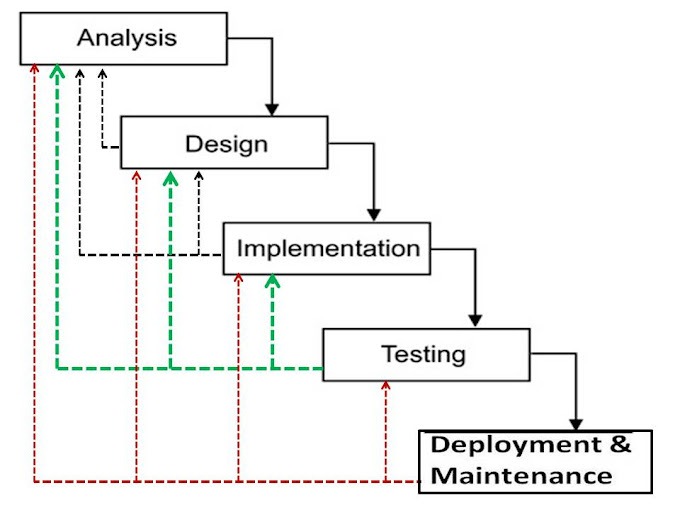
\includegraphics[width=0.6\textwidth]{Images/01 Life_cycle.jpg}  
    \caption{Iterative Waterfall Model}
    \label{Iterative Waterfall Model}  % Label for referencing the figure
\end{figure}

\noindent
The different phases are as follows:

\begin{itemize}
    \item \textbf{Requirement Gathering and Analysis} :
    \noindent
    This initial phase involved understanding the project's goals, objectives, and stakeholder expectations.
    \item \textbf{Data Collection and Preparation} :
    \noindent
    Utilizing Reddit API, the data collection phase was executed. This included downloading the dataset, examining its structure, and performing data cleaning and prepossessing to ensure its suitability for analysis.
    \item \textbf{Model Development} :
    \noindent
    This phase included the creation of a Bag of Words model, splitting the dataset into training and test sets, and implementing various machine learning algorithms.
    \item \textbf{Model Evaluation} :
    \noindent
    Following model development, testing and validation of the models were done, ensuring they met the required accuracy benchmarks. This phase involved using performance metrics such as accuracy, precision, recall, and F1-score to evaluate the models' effectiveness.
    \item \textbf{Final Deployment and Documentation} :
    \noindent
    The last phase focused on deploying the best-performing model and creating comprehensive documentation. This included user manuals and technical documentation to facilitate future maintenance and enhancements.
\end{itemize}


\subsection{Dependencies and Milestones} 
\noindent
Key dependencies were identified for successful project progression. For instance, completion of the data preparation phase was critical before proceeding to model development. Milestones were established at the end of each phase to ensure accountability and track progress. The successful completion of the requirement gathering phase marked the first milestone, followed by the data preparation phase, and so on.

\subsection{Scheduling}
\noindent
Effective scheduling is vital for project success. A detailed timeline with tasks like requirement gathering, data preprocessing, model implementation, and testing was created, with flexibility for adjustments based on feedback. Key milestones, including data analysis, model validation, and user acceptance testing, ensure progress tracking. Using tools like Microsoft Project, we monitor tasks, manage resources, and maintain communication to deliver a high-quality solution on time.

\pagebreak

% Insert MS Project Plan Image
\begin{figure}[h!]  
    \centering
    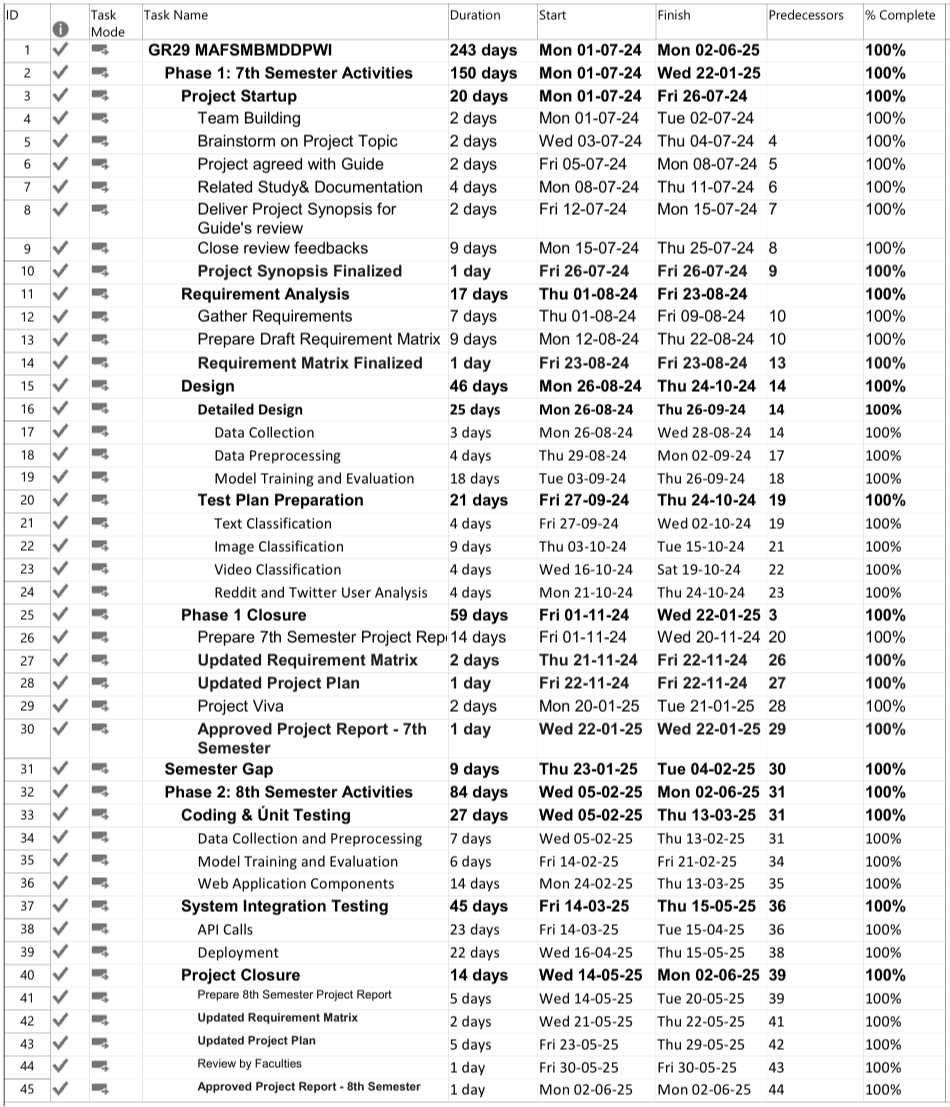
\includegraphics[width=1.0\textwidth]{Images/MS Project Plan Sem 7.png}  
    \caption{Project Plan}
    \label{Project Plan}  % Label for referencing the figure
\end{figure}

\pagebreak

\begin{figure}[h!]  
    \centering
    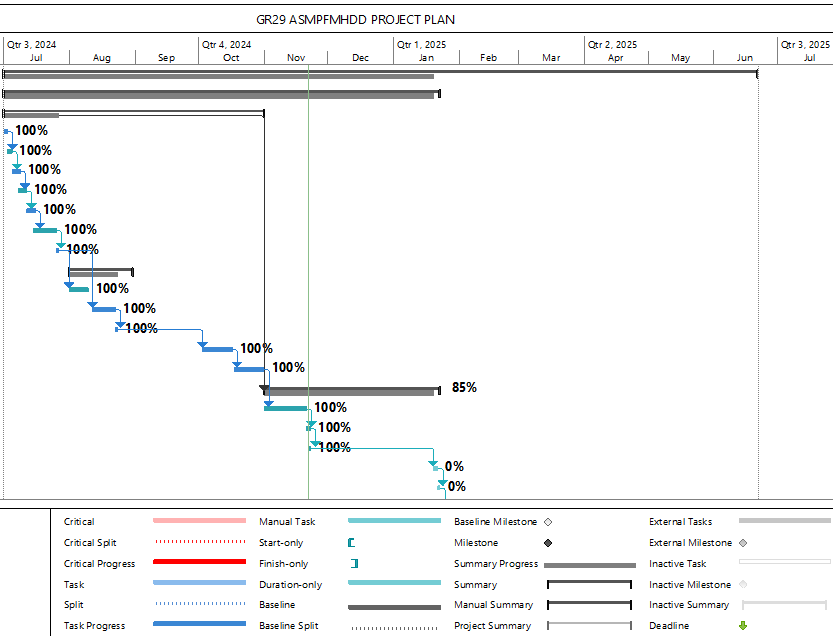
\includegraphics[width=0.79\textwidth]{Images/Gantt Chart.png}  
    \caption{Gantt Chart}
    \label{Gantt Chart}  % Label for referencing the figure
\end{figure}

\pagebreak
% ----------------------- Project Planning ends ------------------------------

% --------------------- Requirement Analysis ---------------------------------
\pagebreak

\section{Requirement Analysis}

\subsection{Requirement Matrix}
% For Requirement Matrix, latest excel should be pasted and formatted here.
\begin{figure}[h!]  
    \centering
    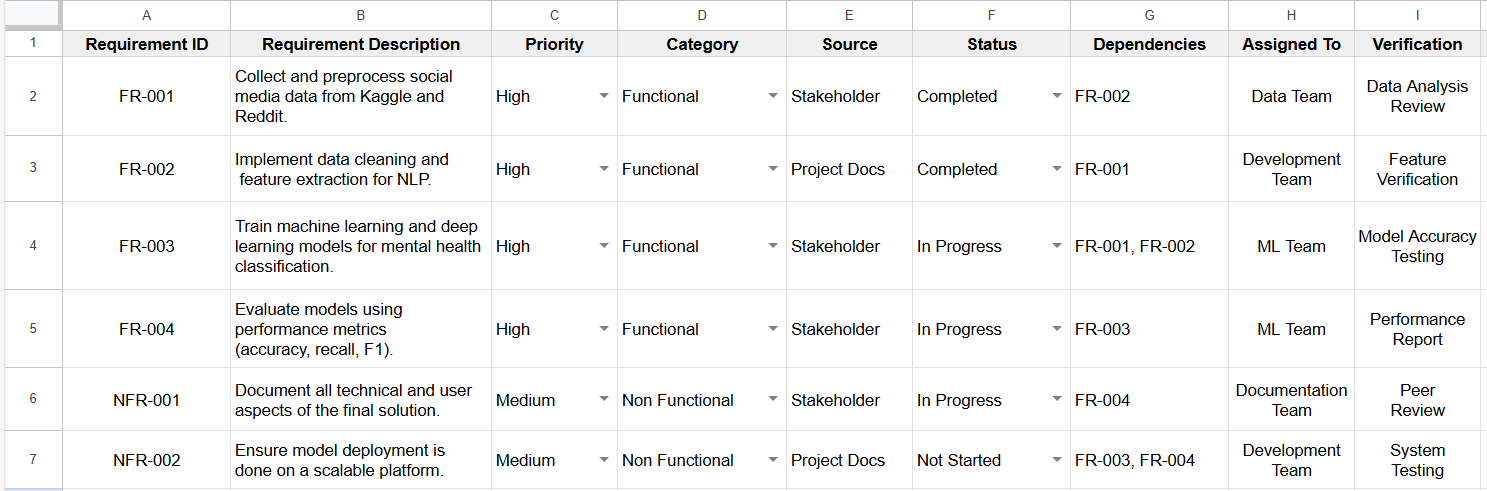
\includegraphics[width=1.0\textwidth]{Images/Requirement Matrix.png}  
    \caption*{Requirement Matrix}
    \label{Requirement Matrix}  % Label for referencing the figure
\end{figure}


\subsection{Requirement Elaboration}
% Create separate sections for separate areas of requirement as in Requirement Matrix. 
% \vspace{.1in}

% \noindent
% For \textbf{Requirement Elaboration}, titles of s6.2.1, 6.2.2 etc. should be with the name of respective requirement areas. Your focus should be on: “What is needed in the system?” Requirement IDs should match with the ID column under Requirement Matrix.

\begin{table}[h]
    \centering
    \renewcommand{\arraystretch}{1.2}
    \begin{tabularx}{\textwidth}{|c|X|X|X|}
        \hline
        \textbf{No} & \textbf{Requirement} & \textbf{Input} & \textbf{Output} \\
        \hline
        FR-001 & Collect social media data from Reddit & API queries & Raw text data \\
        \hline
        FR-002 & Implement data cleaning and preprocessing & Raw text data & Cleaned, structured text \\
        \hline
        FR-003 & Train machine learning and deep learning models & Preprocessed data & Trained models \\
        \hline
        FR-004 & Evaluate models using performance metrics & Trained models & Accuracy, Recall, F1 Score \\
        \hline
        FR-005 & Text Analysis & User text input & Sentiment classification \\
        \hline
        FR-006 & Image Upload Analysis & Uploaded image & Extracted text and sentiment \\
        \hline
        FR-007 & Video Upload Analysis & Uploaded video & Extracted frames and sentiment \\
        \hline
        FR-008 & PDF Upload Analysis & Uploaded PDF & Extracted text and analysis \\
        \hline
        FR-009 & User response to image & User input & Sentiment classification \\
        \hline
        FR-010 & Reddit and Twitter Username Analysis & Username input & User sentiment trends \\
        \hline
        FR-011 & Wellbeing survey and mapping using association matrix & Survey responses & Mental health insights \\
        \hline
        FR-012 & Application Deployment and Model Retraining & Updated dataset & Improved model accuracy within the web application\\
        \hline
        \hline
        NFR-001 & Scalability and Performance & Handling bigger dataset and subset models for a global ensemble model & Maintaining overall accuracy and response time \\
        \hline
    \end{tabularx}
    \caption*{\textbf{Functional and Non-Functional Requirements}}
\end{table}

\pagebreak
% -------------------- Requirement Analysis Ends -----------------------------

% ----------------------------- Design ---------------------------------------

\section{Design}

\subsection{Technical Environment}
% Mention minimum hardware configuration, software tools and package details.
\noindent
The technical environment for the project "Analyzing Social Media Posts for Mental Health Disorder Detection" comprises a combination of hardware, software, and tools that enable smooth data analysis, machine learning model training, and deployment. Below is a detailed overview of the minimum hardware configuration, software tools, and package details necessary to carry out this project effectively. \\

\noindent
\textbf{Minimum Hardware Configuration} \\
\noindent
Given the nature of the project, which involves processing textual data and training machine learning models, the hardware requirements are modest but significant enough to ensure optimal performance. The minimum configuration needed is:
\begin{itemize}
    \item \textbf{Processor} :
    \noindent
    Intel Core i5 (or equivalent) with a base clock speed of at least 2.5 GHz. A multi-core processor is preferred as it helps in parallel processing, which is essential during model training and data preprocessing steps.
    \item \textbf{RAM} :
    \noindent
    8 GB of RAM is recommended to handle the operations of data loading, cleaning, and transformation. Large datasets, like those used in this project, may require more memory to prevent memory overflow errors and reduce delays during processing. For larger datasets, 16 GB of RAM would be ideal.
    \item \textbf{Storage} :
    \noindent
    At least 256 GB of SSD storage is recommended. Faster storage access significantly impacts loading time for datasets and dependencies. SSD is preferred over traditional HDD because of its faster read/write speeds, which benefit large datasets like the Reddit-based social media posts used in this project.
    \item \textbf{Graphics Processing Unit (GPU)} :
    \noindent
    For basic machine learning tasks like Logistic Regression or SVM, a dedicated GPU is not necessary. However, if deep learning models or more complex neural networks were introduced later, a GPU like NVIDIA GTX 1060 with 4 GB VRAM or higher would be advantageous.
    \item \textbf{Operating System} :
    \noindent
    Windows 10 (64-bit) or higher, macOS 10.13 (High Sierra) or higher, or any stable Linux distribution (e.g., Ubuntu 18.04 or higher). The operating system should support all necessary machine learning libraries and be compatible with the tools required for the project.
\end{itemize} 

\noindent
\textbf{Software Tools and Packages} \\
\noindent
For the software stack, the project leverages a set of well-established tools, platforms, and programming libraries to ensure smooth execution from data preprocessing to model deployment:
\begin{itemize}
    \item \textbf{Python} :
    \noindent
    The primary programming language used for data processing, model training, and evaluation. Python is chosen due to its rich ecosystem of libraries and frameworks tailored for machine learning and data science.
    
    \item \textbf{Pandas} :
    \noindent
    A powerful library for data manipulation and analysis, essential for data preprocessing tasks, such as handling missing values and restructuring datasets.
    
    \item \textbf{scikit-learn} :
    \noindent
    A comprehensive machine learning library in Python used for implementing and comparing algorithms in classification, regression, and clustering, along with various model evaluation tools.
    
    \item \textbf{Streamlit} :
    \noindent
    An open-source Python framework that facilitates the deployment of machine learning models and interactive web applications.
    
    \item \textbf{Pyngrok} :
    \noindent
    A Python wrapper for ngrok, used to create secure tunnels to locally deployed applications, which is particularly useful for sharing Streamlit applications over the web.
    
    \item \textbf{Google Colab} :
    \noindent
    A cloud-based platform used for writing, executing, and sharing Python code, with access to GPU and TPU resources, beneficial for model training. It integrates seamlessly with libraries like TensorFlow and PyTorch.
    
    \item \textbf{PRAW (Python Reddit API Wrapper)} :
    \noindent
    A Python library that allows for easy interaction with the Reddit API to access, retrieve, and analyze Reddit data, such as posts, comments, and user information.

    \item \textbf{pytesseract} :
    \noindent
    A Python wrapper for Tesseract OCR, used to extract text from images. It's essential for converting image-based text data into a format suitable for processing.
    
    \item \textbf{Pillow} :
    \noindent
    A Python Imaging Library that adds support for image processing, which aids in handling image files for text recognition tasks with pytesseract.

    \item \textbf{joblib} :
    \noindent
    A library for efficient serialization and deserialization of Python objects, especially useful for saving and loading machine learning models during deployment.
    
    \item \textbf{protobuf} :
    \noindent
    A protocol buffer library by Google used for serializing structured data, helpful in efficient data exchange between applications.
    
    \item \textbf{deep-translator} :
    \noindent
    A library that facilitates easy translation across different languages, enabling multilingual processing of text data.
    
    \item \textbf{Requests} :
    \noindent
    A user-friendly library for making HTTP requests, used to retrieve data from APIs or web resources as part of data collection.
    
    \item \textbf{google-generativeai} :
    \noindent
    A Python client library for Google’s generative AI models, providing tools to integrate and utilize AI functionalities within the project.
    
\end{itemize}


\subsection{Hierarchy of Modules}
% Provide a diagram.
\begin{figure}[h!]  
    \centering
    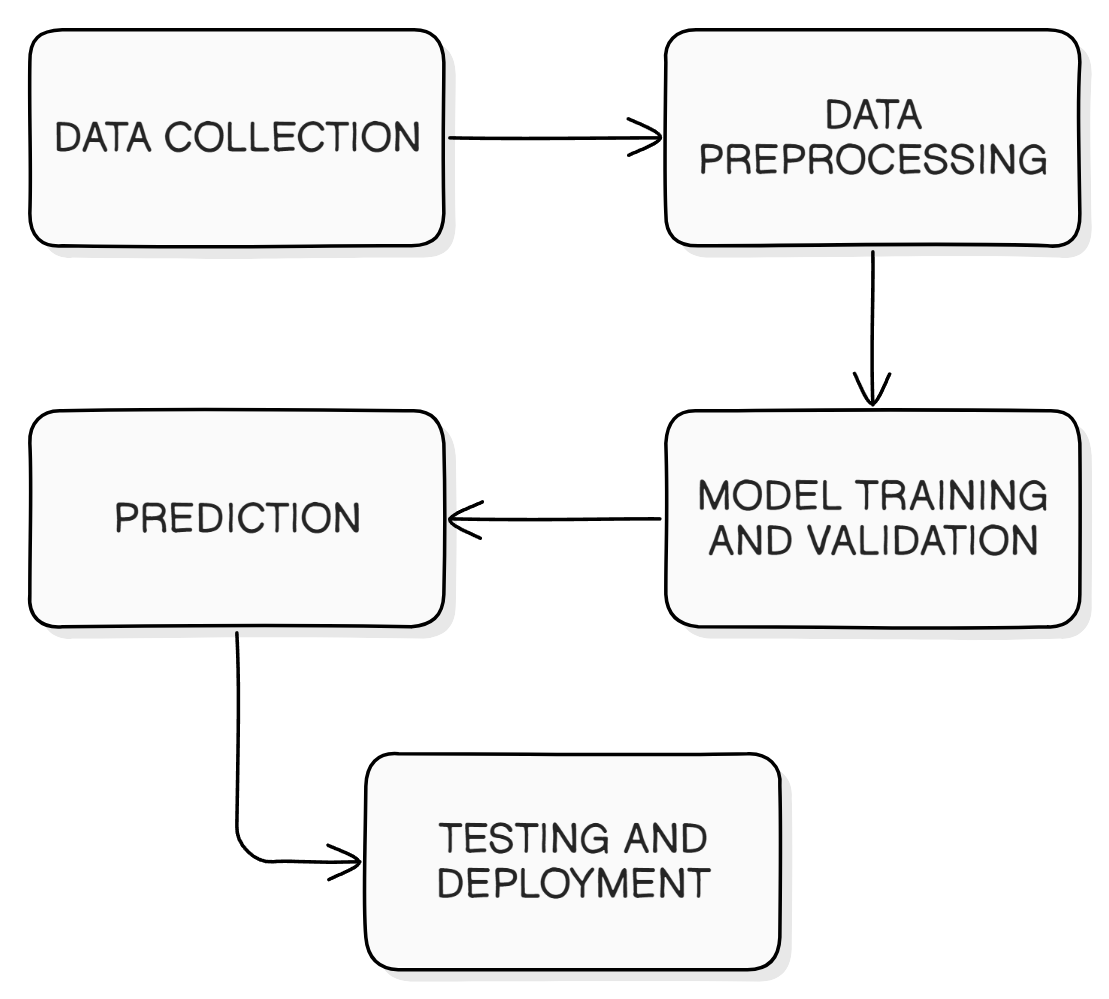
\includegraphics[width=0.6\textwidth]{Images/Project Modules.png}  
    \caption{Project Modules}
    \label{Project Modules}  % Label for referencing the figure
\end{figure}

\noindent
In this project, the system is structured into key modules to classify mental health issues based on text input effectively. The \textbf{Data Collection Module} gathers relevant text data, building a comprehensive dataset from sources like CSV files or platforms such as Reddit via PRAW. Next, the \textbf{Data Preprocessing Module} loads and cleans this data through tokenization, stop-word removal, and lemmatization, preparing it for analysis. Following this, the \textbf{Model Training and Validation Module} converts the text into numerical features using techniques like TF-IDF, splitting the data into training and validation sets to test various machine learning models, including Logistic Regression, Naive Bayes, SVM, Random Forest, XGboost and LSTM. Finally, the \textbf{Testing and Deployment Module} allows real-time predictions by deploying the model on platforms like Streamlit Cloud, providing an accessible solution for practical applications.

\subsection{Detailed Design}
% Provide hierarchy of modules or overall system diagram. 
% \vspace{.1in}
\begin{figure}[h!]  
    \centering
    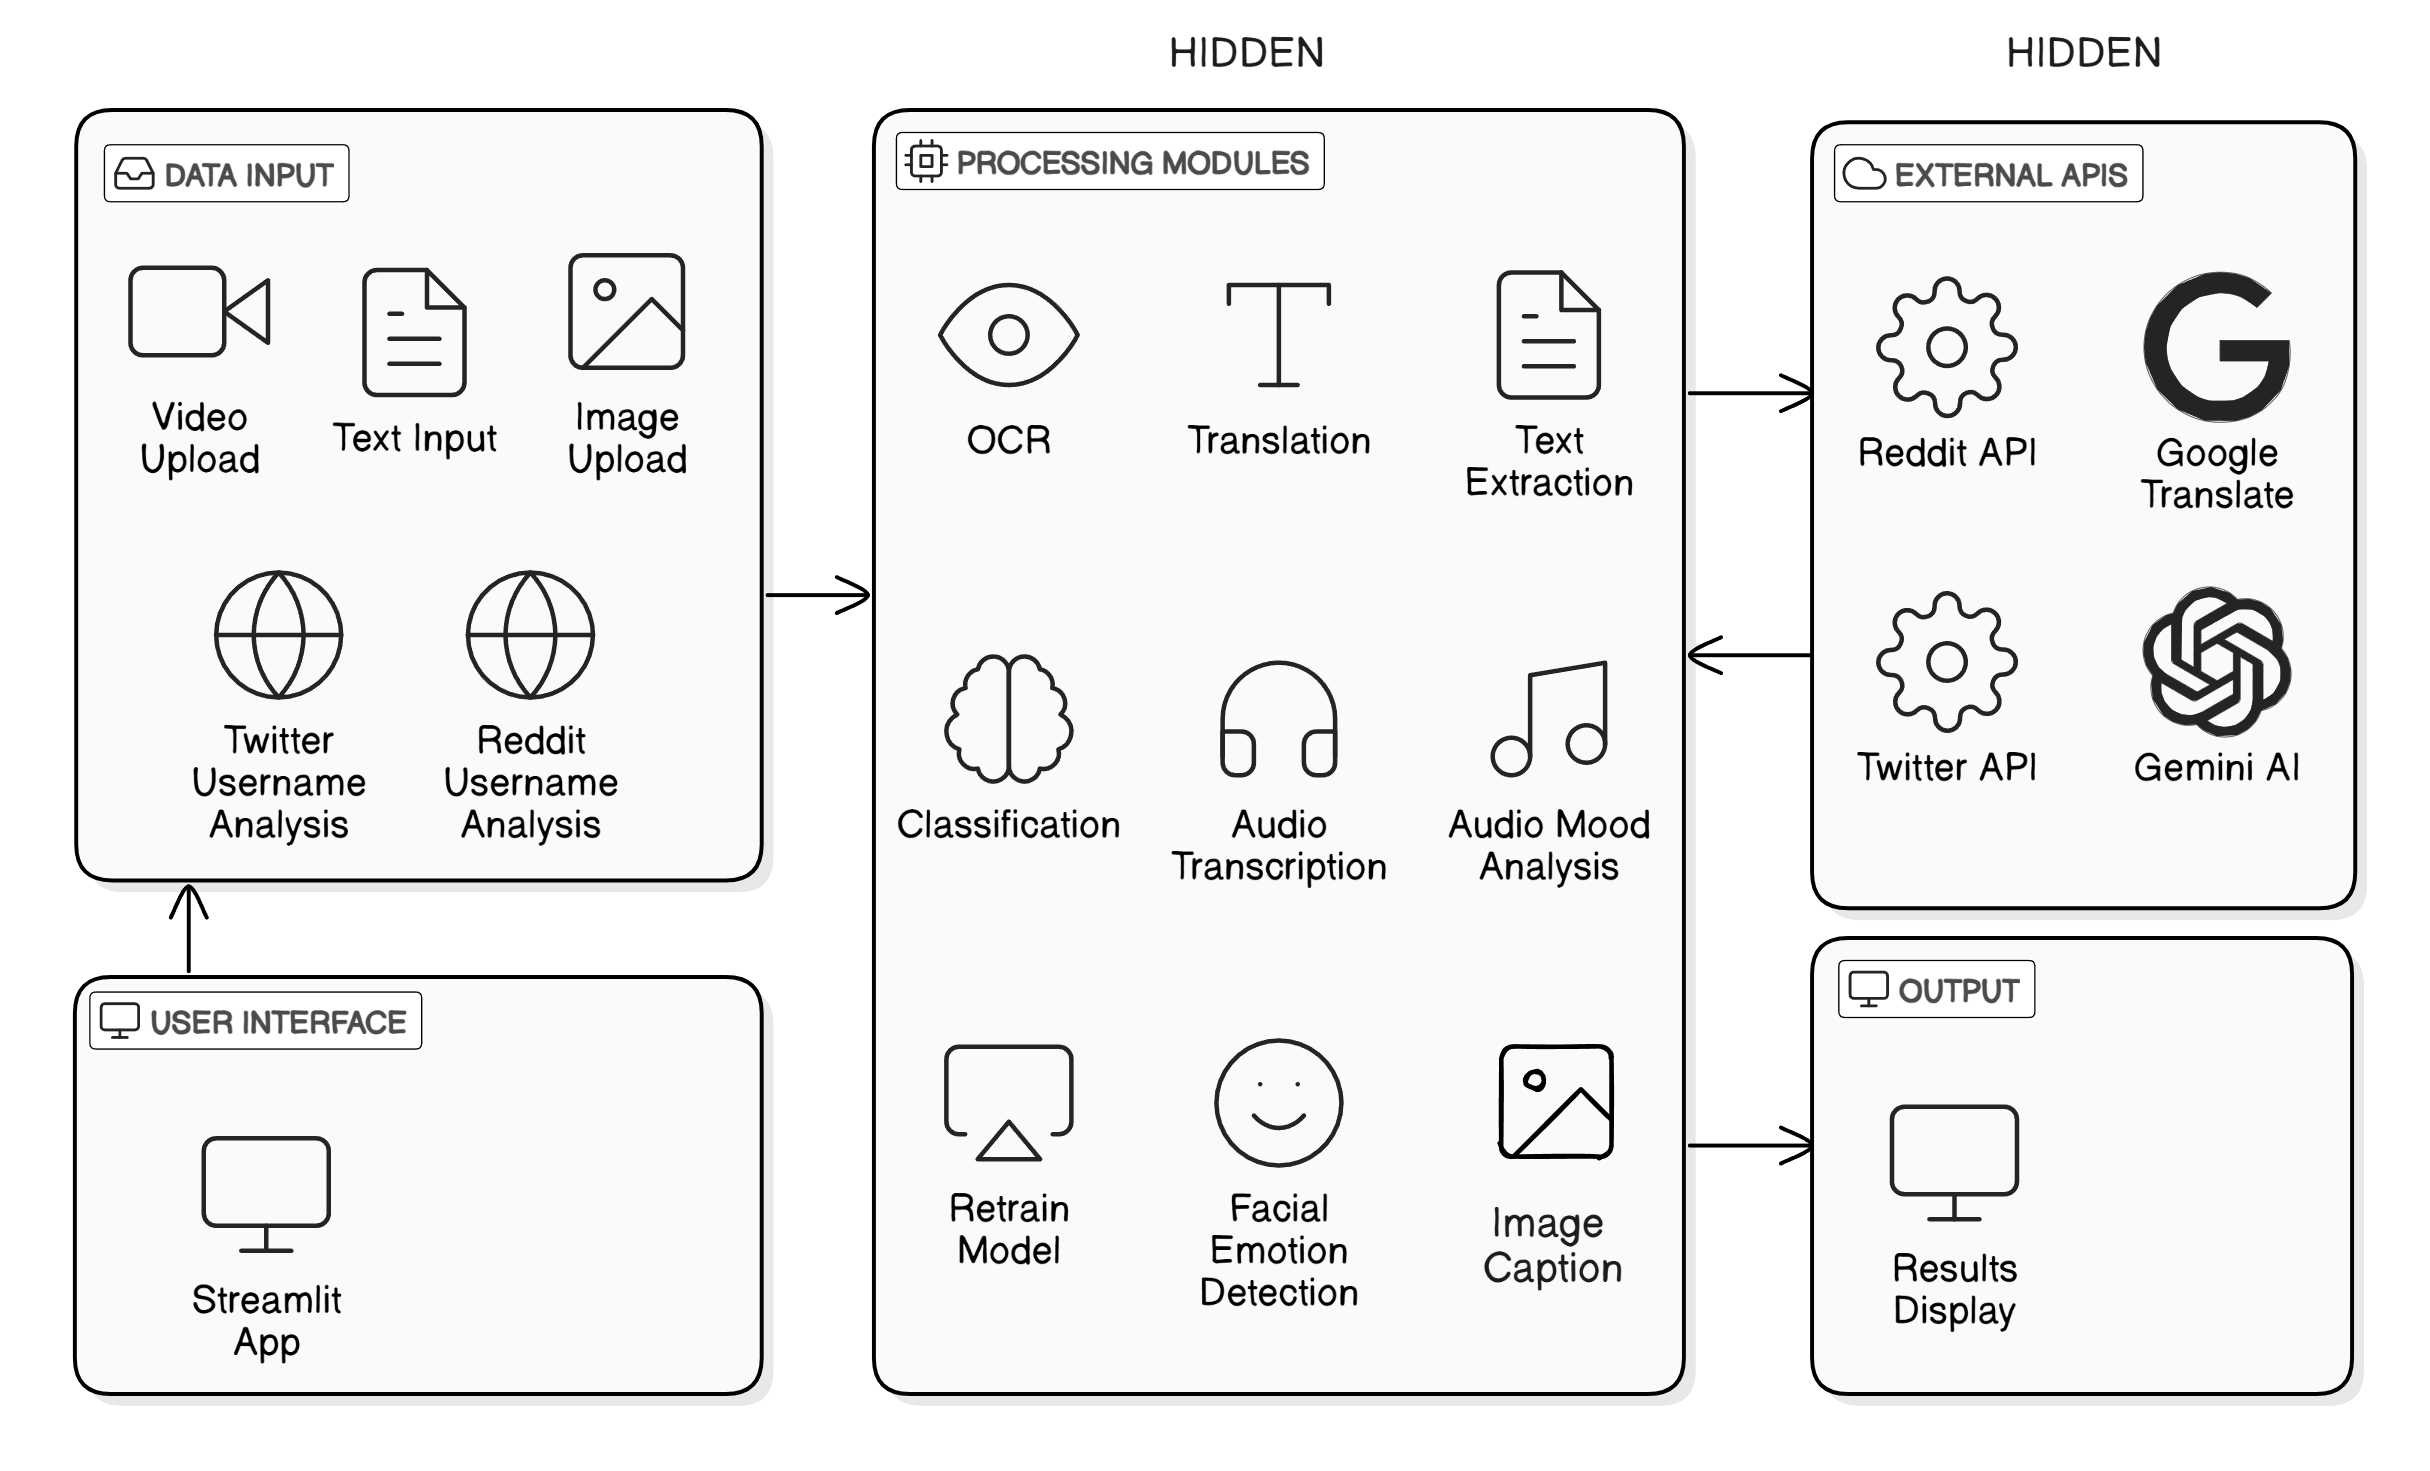
\includegraphics[width=1.0\textwidth]{Images/System Overview.png}  
    \caption{System Overview}
    \label{System Overview}  % Label for referencing the figure
\end{figure}

\begin{figure}[h!]  
    \centering
    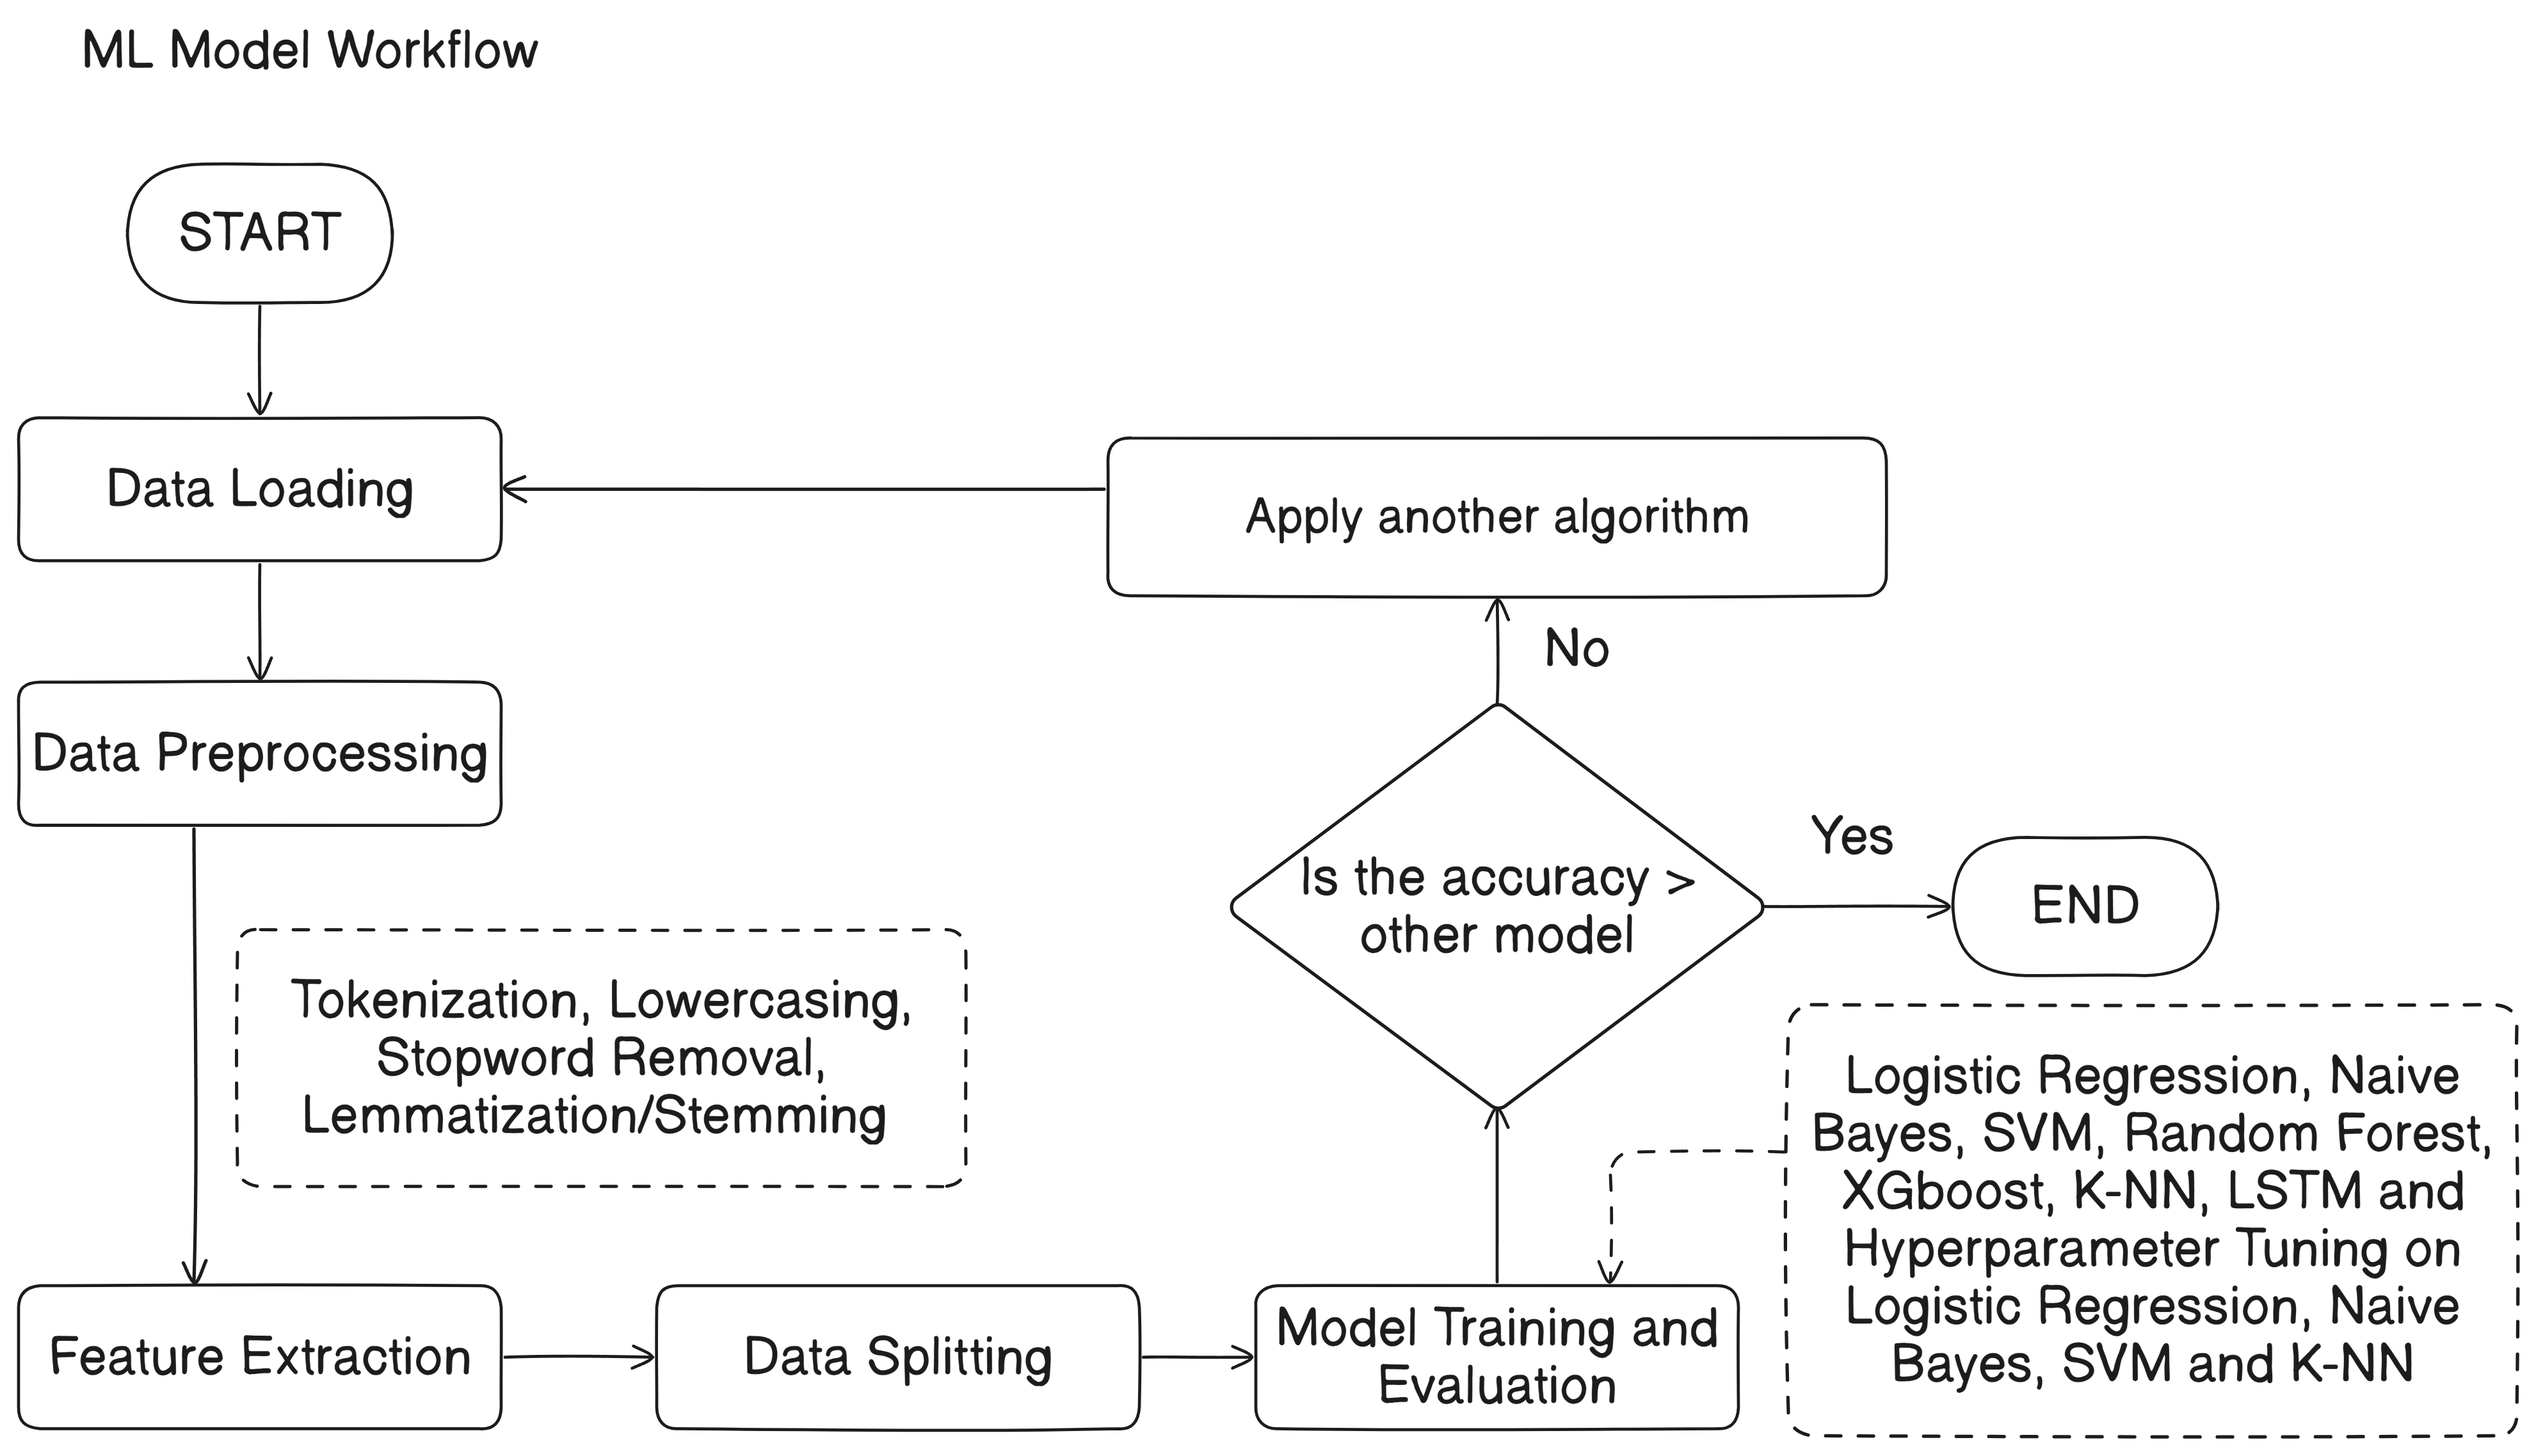
\includegraphics[width=1.0\textwidth]{Images/ML Model Workflow.png}  
    \caption{Model Workflow}
    \label{Model Workflow}  % Label for referencing the figure
\end{figure}

% \noindent
% For Detailed Design, use flowcharts, DFD, UML or ER diagrams as applicable. Titles of s7.2.1, 7.2.2 etc. should be with the name of respective design modules. Your focus should be on: “How the requirement will be implemented in the system?” Design Reference subsection numbers should be matching as stated in Requirement Matrix.
\vspace{.1in}

\subsubsection{Data Loading and Preprocessing}
\noindent
The Data Loading and Preprocessing Module is the foundation of the system, responsible for ingesting and preparing the text data for analysis. This module begins by loading the dataset from the preprocessed\_mental\_health\_text.csv file, which contains various mental health-related text entries. Once the data is loaded, a series of preprocessing steps are conducted to ensure the text is clean and ready for feature extraction. This includes tokenization, where the text is split into individual words or tokens, and lowercasing to maintain uniformity across the dataset. Additionally, stop-word removal is performed to eliminate common words that do not contribute to the meaning, such as "and," "the," and "is." Finally, lemmatization or stemming is applied to reduce words to their base or root forms. These preprocessing techniques are crucial as they help improve the quality of the input data, ultimately leading to better model performance.

\subsubsection{Feature Extraction}
\noindent
In the Feature Extraction Module, the preprocessed text data is transformed into a numerical format that machine learning algorithms can process. This module allows for the selection between two primary feature extraction methods: Term Frequency-Inverse Document Frequency (TF-IDF). The TF-IDF approach evaluates the importance of words in the dataset by considering their frequency in individual documents relative to their overall occurrence across all documents. This helps in highlighting the most informative words. By converting text into numerical features, this module prepares the data for the subsequent training and validation stages, ensuring that the classification models can effectively interpret the input.

\subsubsection{Model Training and Validation}
\noindent
The Model Training and Validation Module is critical to developing a robust classification system. In this module, the dataset is split into training and testing sets to evaluate the performance of the models accurately. Various classification algorithms are employed, including Logistic Regression, Naive Bayes, Support Vector Machines, Random Forest, XGboost, K-Nearest-Neighbours and LSTM. Each model is trained on the training set, which involves adjusting the model parameters based on the input features and their corresponding labels. Following training, the models undergo validation to assess their performance using various metrics such as accuracy, precision, recall, and F1-score. A decision point is included to determine if the achieved accuracy meets the project requirements. If the accuracy is deemed acceptable, the model is accepted. 

\subsubsection{Prediction}
\noindent
The Prediction Module is designed to provide real-time classification of new input text related to mental health issues. Upon receiving user input, this module initiates a preprocessing workflow that mirrors the steps applied during the training phase, including tokenization, lowercasing, stop-word removal, and lemmatization or stemming. Once the input text is preprocessed, it is fed into the trained classification models to generate predictions. Each model may provide a classification result, allowing for a comprehensive analysis of the input. This module not only delivers the predicted mental health issue but also ensures that users receive an informative output that reflects the confidence level of each prediction, enabling them to understand the model's reasoning.

\subsubsection{Testing and Deployment}
\noindent
The module focuses on making the trained models accessible for real-time predictions. Once the models have been validated and selected based on their performance, this module prepares them for deployment on suitable platforms like Streamlit Cloud. This involves packaging the models and creating a user interface where users can input text and receive predictions. The deployment process also includes considerations for scaling, ensuring that the system can handle multiple requests simultaneously while maintaining responsiveness. By providing a free and efficient deployment solution, this module enables users to access the mental health classification service easily. The deployment of the models ensures that the insights generated from the analysis can be utilized effectively in real-world applications.

\begin{figure}[h!]  
    \centering
    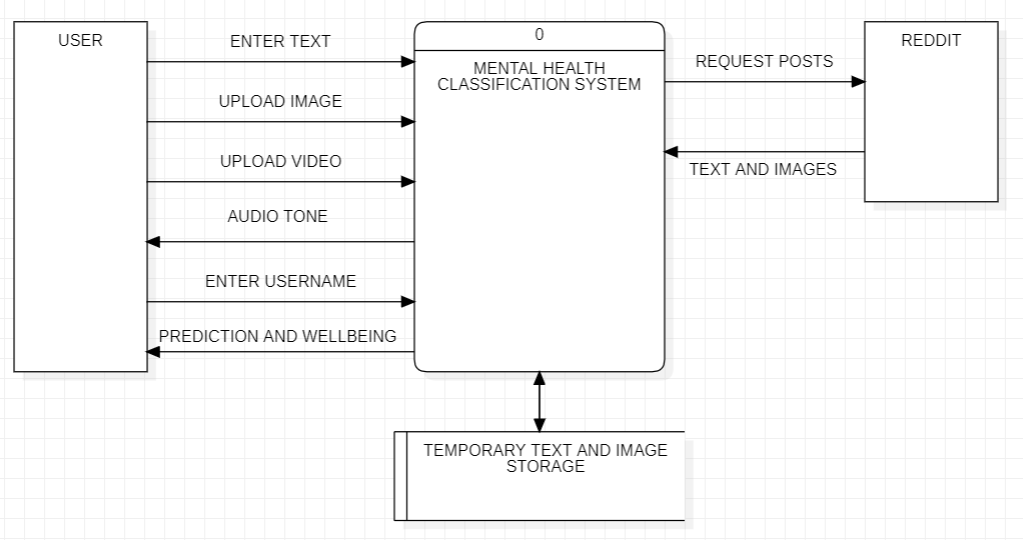
\includegraphics[width=0.9\textwidth]{Images/DFD L0.png}  
    \caption{DFD Level 0 of the System}
    \label{dfdl0123}  % Label for referencing the figure
\end{figure}


\begin{figure}[h!]  
    \centering
    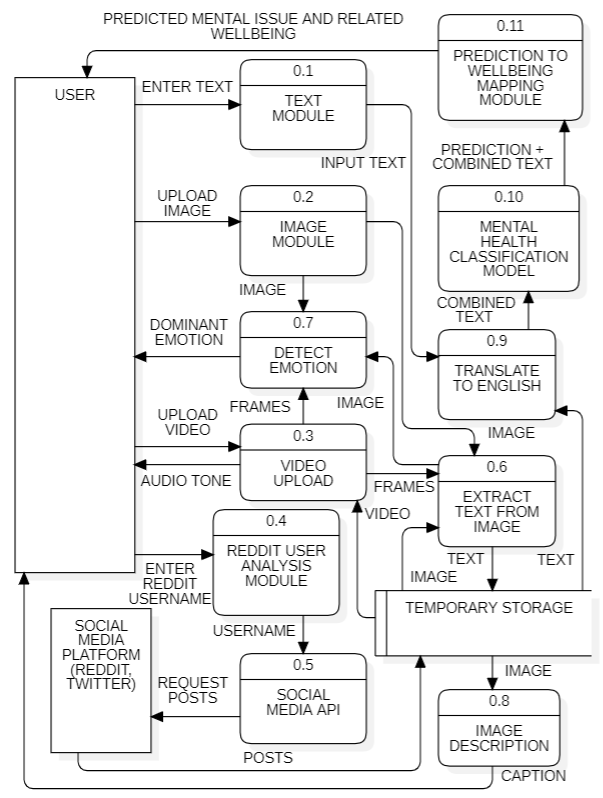
\includegraphics[width=1.0\textwidth]{Images/DFD L1.png}  
    \caption{DFD Level 1 of the System}
    \label{dfdl1234}  % Label for referencing the figure
\end{figure}


\subsection{Emotion Detection Functionality}

\begin{figure}[h!]  
    \centering
    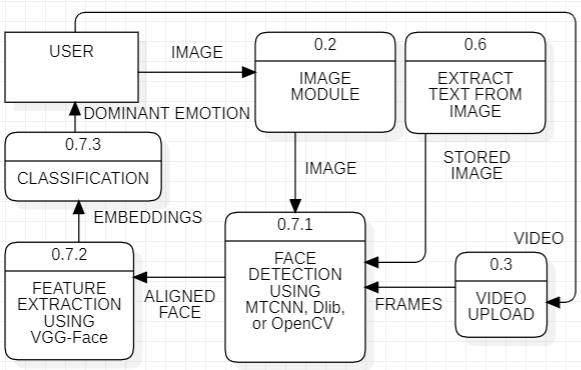
\includegraphics[width=1.0\textwidth]{Images/DFD L2 EMOTION.png}  
    \caption{DFD Level 2 of Emotion Detection Functionality}
    \label{dfdl14456}  % Label for referencing the figure
\end{figure}

\noindent
DeepFace analysis involves several steps to process and analyze facial features from an uploaded image or video frame. The process begins with the user uploading the input, which is passed to DeepFace’s pipeline. The first step is face detection, where models like MTCNN, Dlib, or OpenCV locate faces within the image. MTCNN (Multi-task Cascaded Convolutional Networks) detects faces using cascaded CNNs for high accuracy and alignment, while Dlib employs histogram-oriented gradients and machine learning techniques for robust detection. OpenCV, a widely-used computer vision library, uses Haar cascades or DNN-based approaches to detect faces. Once detected, the faces are cropped and aligned for consistency. Next is feature extraction, where pre-trained models like VGG-Face (a deep CNN trained specifically for face recognition) or Facenet (which uses triplet loss to generate highly discriminative face embeddings) convert the aligned face into numerical vectors called embeddings. These embeddings are compared using techniques like cosine similarity or Euclidean distance for tasks such as emotion detection(e.g., happiness, sadness), demographic analysis (e.g., age, gender), or face verification (matching two faces). Finally, the results, such as detected emotions or attributes, are displayed to the user, completing the analysis pipeline.


\subsection{Extract Text From Image}

\begin{figure}[h!]  
    \centering
    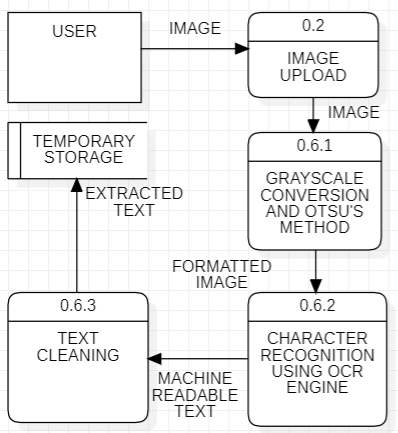
\includegraphics[width=0.7\textwidth]{Images/DFD L2 TEXT EXTRACT.png}  
    \caption{DFD Level 2 of Text Extraction from Image}
    \label{dfdl13456}  % Label for referencing the figure
\end{figure}

\noindent
The process of extracting text from an image using Tesseract-OCR begins with the user uploading an image containing text, such as a scanned document or a photo of a sign. This raw input undergoes preprocessing to enhance the image for OCR recognition. The first step in preprocessing is grayscale conversion, where the image’s RGB values are reduced to a single intensity value using a weighted formula. This simplifies the image by removing color information while retaining the text regions. Next, noise reduction is applied using techniques like Gaussian Blur or Median Blur, which smooth out artifacts while preserving the edges of text. After noise reduction, binarization is performed to convert the grayscale image into a binary format (black-and-white) using methods like Otsu’s thresholding. This step isolates the text from the background. Region detection follows, where text-heavy areas are identified using contour detection or connected component analysis, filtering out non-text regions based on properties like aspect ratio and alignment. Once preprocessing is complete, the image is passed to Tesseract for character recognition. This involves segmenting the image into text lines and individual characters, which are then processed by Tesseract’s LSTM-based neural network. The network evaluates sequences of characters in context, improving the accuracy of word recognition. Recognized characters are combined into machine-readable text, leveraging language models and dictionary lookups to maintain the natural flow and correct structure of the text. The output is a string of recognized text, but it may still require postprocessing for better accuracy and readability. Postprocessing begins with error correction, where the recognized text is compared against dictionaries or spell-checking algorithms to identify and fix errors caused by OCR misrecognition. Rule-based corrections are also applied, such as replacing common misinterpreted characters (e.g., \`0\` with \`O\` or \`l\` with \`1\`) depending on the context. After error correction, formatting is applied to structure the text into paragraphs, reconstruct line breaks, and retain alignments. This ensures that the extracted text is not only accurate but also well-organized for further use. Finally, the extracted text is either displayed to the user or saved to a file format such as \`.txt\` or \`.docx\`. This structured and cleaned output can then be utilized for various applications, from document analysis to content storage. The entire pipeline, from preprocessing to postprocessing, ensures a high-quality extraction process by combining image enhancement, deep learning-based recognition, and advanced text correction methods.


\subsection{Image Description}

\begin{figure}[h!]  
    \centering
    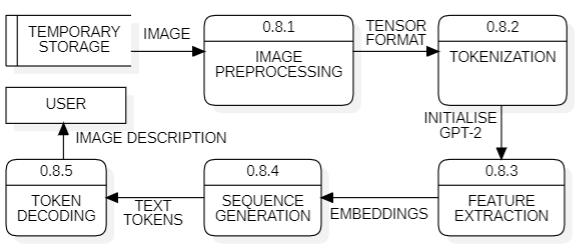
\includegraphics[width=0.9\textwidth]{Images/DFD L2 ID.png}  
    \caption{DFD Level 2 of Image Description}
    \label{dfdl122}  % Label for referencing the figure
\end{figure}

\noindent
The process of generating an image description using Python’s Transformers module and the ViT-GPT2 model begins with the user input, where the user uploads an image to be described. This image can be in any format (e.g., PNG, JPEG), and it is the raw data that will undergo a series of transformations before the description is generated. Once the image is received, it proceeds to the preprocessing stage. Preprocessing involves multiple steps: first, the image is resized to match the input dimensions required by the Vision Transformer (ViT) model, typically \(224 \times 224\) pixels. This ensures uniformity across all input data. The pixel values are then normalized to fall within a standard range (e.g., between 0 and 1), which improves the efficiency and stability of the model's computations. The image is subsequently transformed into a tensor format, which is the data structure required for processing by PyTorch or TensorFlow-based deep learning models. At this stage, the **GPT-2 tokenizer** is also initialized, preparing it to convert tokens into text during the sequence generation phase. Following preprocessing, the system moves to feature extraction, where the Vision Transformer (ViT) processes the image to extract meaningful features. ViT divides the image into smaller patches, typically \(16 \times 16\) pixels, and flattens each patch into a vector. These vectors are embedded using a linear projection layer, and positional embeddings are added to encode the spatial arrangement of the patches. The embedded patches are then passed through several transformer layers, where self-attention mechanisms analyze relationships between patches to capture both local and global image features. The final output of ViT is a high-dimensional embedding vector that represents the visual content of the image. This embedding vector is then passed to the GPT-2 decoder for the sequence generation phase. GPT-2 uses the image embeddings as input and applies its pre-trained language model to generate a sequence of text tokens. This is achieved through an iterative process where GPT-2 predicts the next token in the sequence based on the embeddings and previously generated tokens. The model continues this process until it reaches a stopping condition, such as an end-of-sequence (EOS) token. The generated tokens are numerical representations of words and phrases. Next comes the postprocessing stage, where the numerical tokens generated by GPT-2 are decoded back into human-readable text using the GPT-2 tokenizer. This step involves mapping the numerical tokens to their corresponding words in the vocabulary. The decoded text is then cleaned up for readability, ensuring proper grammar and structure. Any formatting issues are addressed during this stage to produce coherent and meaningful sentences. Finally, the system outputs the image description to the user. The description is a concise and accurate textual representation of the image content, such as “A group of people playing soccer on a field.” This description can be displayed on the application’s interface or saved to a file for further use. By leveraging the advanced capabilities of the Vision Transformer for feature extraction and GPT-2 for language modeling, this pipeline provides an efficient and accurate solution for automated image captioning.


\subsection{Translation to English}

\begin{figure}[h!]  
    \centering
    \includegraphics[width=0.9\textwidth]{Images/DFD L2 TE.png}  
    \caption{DFD Level 2 of Translation to English}
    \label{dfdl111}  % Label for referencing the figure
\end{figure}

\noindent
The process of translating text to English using DeepTranslator begins with the user providing input, either by typing text in a non-English language or uploading a file containing text. This input is handled by the system, which prepares it for translation. The text is first preprocessed to ensure optimal translation results. This involves cleaning the input by removing unwanted characters such as extra whitespace, punctuation errors, or HTML tags that could interfere with accurate translation. If the source language is not specified, a language detection step is performed. This step uses machine learning models trained on multilingual datasets to analyze patterns in the text, such as character distribution and word frequency, to determine the language. Models like Google’s Compact Language Detector employ statistical and supervised learning methods for this purpose. Once the text is prepared, it is passed to the DeepTranslator module, which interfaces with translation APIs like Google Translate or Microsoft Translator. These APIs rely on advanced neural machine translation (NMT) techniques to perform the translation. NMT models, which are based on deep learning, use sequence-to-sequence (seq2seq) architectures with encoder-decoder frameworks. The encoder processes the input text and converts it into a latent representation, a numerical vector capturing its meaning. This representation is then passed to the decoder, which generates the translated text in English. To ensure contextual accuracy, these models utilize attention mechanisms, which help focus on relevant parts of the input sentence during translation. Modern transformer-based architectures, like those used in Google Translate, enhance translation performance by enabling parallel processing of text and capturing long-range dependencies in sentences. After translation, the system postprocesses the output to ensure quality and readability. This includes validating the translated text for completeness, handling errors like untranslated phrases, and retrying failed requests if necessary. The output is formatted to resemble the original structure of the input, preserving elements like paragraphs, line breaks, and punctuation to maintain coherence. Finally, the translated text is displayed or saved, ensuring it is clean, accurate, and easy to understand. Throughout this process, concepts from natural language processing (NLP), deep learning, and robust error handling are integrated to provide reliable and efficient translations.


\subsection{Prediction to Wellbeing Mapping}

\begin{figure}[h!]  
    \centering
    \includegraphics[width=0.9\textwidth]{Images/DFD L2 MW.png}  
    \caption{DFD Level 2 of Prediction to Wellbeing Mapping}
    \label{dfdl166}  % Label for referencing the figure
\end{figure}

\noindent
The process begins when the user provides input data for prediction, which could be in the form of text, behavioral data, or health metrics. For instance, a user might input their mood and health conditions, share behavioral patterns, or upload relevant data such as physical activity logs or medical records. This data serves as the foundation for predicting the user's mental health or overall wellbeing. Once the data is provided, the next step is preprocessing, which involves cleaning and transforming the raw input. During the data cleaning phase, any noise, missing values, or redundant information are identified and removed. This ensures the dataset is clean and ready for processing. Additionally, feature engineering is performed to extract meaningful attributes or characteristics from the raw data. For example, from behavioral data, features like activity frequency or sleep patterns may be derived. This allows the model to work with relevant information that enhances the prediction process. The third step involves embedding generation, where the core model, GEMINI 1.5 FLASH, processes the preprocessed input to generate embeddings. Embeddings are high-dimensional vectors that capture the semantic and contextual properties of the data. For example, when analyzing text input, GEMINI 1.5 FLASH uses its deep learning algorithms to understand the context and meaning of the user's words, transforming them into embeddings that encapsulate both the surface-level meaning and the deeper nuances of the data. This representation of the input data is essential for subsequent prediction tasks. In the prediction model phase, the generated embeddings are passed to machine learning models, which use these embeddings to predict a user's mental health status or behavioral outcomes. These models may utilize various algorithms, such as decision trees, support vector machines, or deep learning models, to make predictions. The system not only predicts the mental health condition but also maps these predictions to various wellbeing dimensions. These dimensions could include emotional wellbeing, such as happiness or stress; physical wellbeing, like energy levels or fatigue; and social wellbeing, including aspects like connectedness or isolation. By doing so, the system offers a comprehensive view of the user's overall wellbeing based on the predictions. Once predictions are made, postprocessing ensures the results are accurate and formatted properly. During the validation phase, the predictions are checked for any anomalies or inconsistencies, ensuring the output is reliable. This might involve techniques like consistency checks or outlier detection to verify that the predictions align with expected patterns. After validation, the results are formatted into a user-friendly structure. This might include organizing the wellbeing data into clear categories, such as emotional, physical, and social wellbeing, making it easy for the user to interpret. Finally, the system delivers the output, displaying or saving the prediction and associated wellbeing mapping. This output is presented in a way that helps the user understand the various aspects of their mental and physical health, giving them insights into their current state of wellbeing and providing actionable data for improvement.


\subsection{Audio Mood Analysis}

\begin{figure}[h!]  
    \centering
    \includegraphics[width=0.9\textwidth]{Images/DFD L2 AM.png}  
    \caption{DFD Level 2 of Audio Mood Analysis}
    \label{dfdl671}  % Label for referencing the figure
\end{figure}

\noindent
The analyze\_audio\_mood function begins with the user providing a path to a video file as input. This is the starting point of the process where the user supplies the video from which the audio will be extracted. In the preprocessing stage, the video file is passed to the extract\_audio\_from\_video function. This function extracts the audio content from the video, separating it for further analysis. Once the audio is extracted, the next step involves loading the audio file into memory using the librosa library, which prepares the audio data for feature extraction. The core of the audio processing happens during the MFCC (Mel-frequency cepstral coefficients) feature extraction. The librosa.feature.mfcc method is used to compute the MFCCs of the audio. These MFCCs represent different frequency bands of the audio signal and are crucial for analyzing the characteristics of the audio that correspond to various emotional tones. By capturing frequency patterns, MFCCs provide a robust feature set for mood classification. After the MFCCs are extracted, the next step is feature segmentation. The MFCC array is divided into four distinct frequency bands: low frequencies (MFCCs 0, 1, and 2), mid-low frequencies (MFCCs 3 and 4), mid-high frequencies (MFCCs 5, 6, and 7), and high frequencies (MFCCs 8, 9, 10, 11, and 12). For each of these frequency bands, the scalar mean of the MFCC values is computed. This scalar mean represents the overall intensity of the audio in each frequency range, simplifying the data for classification purposes. Finally, the mood classification process takes place. The scalar means for each of the frequency bands are compared to determine the dominant mood of the audio. Based on these comparisons, the function classifies the audio as normal, neutral, melancholic, calm, anxious, or happy, depending on which frequency bands exhibit the strongest characteristics. This mood classification is then returned as the result of the analysis.



\vspace{2em}

\noindent
The various processes and technologies discussed throughout this conversation can play a pivotal role in enhancing the classification and prediction of mental health disorders. The use of machine learning (ML) and deep learning (DL) models enables the system to process and analyze large volumes of data, such as text, behavioral patterns, health metrics, and even multimedia inputs (e.g., images, audio, and video). By leveraging the DeepFace module for facial emotion recognition, the system can identify emotional cues from visual data, helping to assess a user’s emotional state. This is complemented by text analysis models, such as those built with Logistic Regression, k-NN, SVM, and LSTM architectures, which are capable of classifying mental health issues from user-provided text, such as social media posts, personal narratives, or other forms of written communication.

\vspace{2em}

\noindent
Further enhancing the capability, the integration of DeepTranslator ensures that non-English input can be translated into English, allowing the system to support a wider variety of users and ensuring the accuracy of the mental health analysis, even when the data comes from different languages. Meanwhile, behavioral data and health metrics are crucial inputs that can provide insights into a person’s overall wellbeing. These data sources are analyzed using GEMINI 1.5 FLASH, which generates embeddings capturing the semantic and contextual properties of the input data, feeding into prediction models that classify users' mental health conditions and map them to various wellbeing dimensions. The classification of conditions like anxiety, depression, PTSD, and others can be made more accurate through these comprehensive data analyses.

\vspace{2em}

\noindent
By incorporating audio mood analysis through techniques such as MFCC for audio emotion detection and facial expression recognition for video inputs, the system further refines its ability to assess emotional and mental states. These audio and visual analyses provide additional layers of understanding that text alone might not fully capture. In conjunction with these features, streaming data from social media platforms like Reddit or Twitter allows for the monitoring of a user’s public posts, providing real-time insights into their mental health as they interact with others online.

\vspace{2em}

\noindent
The combined use of these models and processes facilitates a holistic approach to mental health disorder classification. The system can classify mental health issues based on a range of factors, including written text, emotional tone from images, behavioral patterns, and audio cues. This multimodal approach helps create a more comprehensive, accurate, and nuanced prediction of mental health conditions, offering personalized insights into emotional, physical, and social wellbeing. As a result, users benefit from a system that not only detects potential mental health issues but also offers a deeper understanding of their overall wellbeing, which can inform targeted interventions, support, and wellbeing strategies.



% \noindent
% Create separate sections for separate modules of design as in Requirement Matrix. Ensure to provide Design Diagrams \textit{(e.g. System overview / DFDs / ERDs etc.; cross-reference to be drawn from Chapter 6), Decision matrix (for algorithm recommendation etc.) }




% \subsubsection{Name of Design Module 1 \label{sec:design_mod1}}
% \subsubsection{Name of Design Module 2 \label{sec:design_mod2}}
% \subsubsection{Name of Design Module 3 etc \label{sec:design_mod3}}


% Refer APPENDIX A  – Prototypes \ref{sec:proto} for prototype details.


% ------------------------------ Design Ends ---------------------------------


% --------------------------- Implementation ---------------------------------


\section{Implementation}

\begin{figure}[h!]  
    \centering
    \includegraphics[width=1.0\textwidth]{Images/ML Model Workflow.png}  
    \caption{Workflow for getting the model for the web application}
    \label{model workflow}  % Label for referencing the figure
\end{figure}


\subsection{Data Collection and Dataset Preparation}
\begin{table}[H]
    \centering
    \caption*{Stepwise Algorithm for Data Collection and Dataset Combination}
    \label{tab:algorithm}
    \begin{tabularx}{\textwidth}{|c|X|}
        \hline
        \textbf{Step} & \textbf{Description} \\
        \hline
        1 & \textbf{Import Libraries:} Import \texttt{praw, pandas, time} for data collection and \texttt{sklearn.utils.shuffle} for combining datasets. \\
        \hline
        2 & \textbf{Initialize Reddit API:} Use the provided credentials (\texttt{client\_id}, \texttt{client\_secret}, \texttt{user\_agent}) to create a Reddit instance. \\
        \hline
        3 & \textbf{Define Subreddits and Labels:} Create a dictionary mapping labels to subreddit lists:
            \begin{itemize}[noitemsep, topsep=0pt]
                \item \textbf{normal}: \texttt{news, AskReddit}
                \item \textbf{depression}: \texttt{depression}
                \item \textbf{ptsd}: \texttt{PTSD}
                \item \textbf{anxiety}: \texttt{Anxiety}
                \item \textbf{bipolar}: \texttt{BipolarReddit}
            \end{itemize} \\
        \hline
        4 & \textbf{Set Post Types and Limit:} Define post types (\texttt{hot, new, top}) and set \texttt{posts\_per\_type} to 100. \\
        \hline
        5 & \textbf{Collect Posts:}
            \begin{itemize}[noitemsep, topsep=0pt]
                \item For each label and its associated subreddits, iterate over each post type.
                \item Retrieve posts from the subreddit (using the corresponding post type and a limit of 100).
                \item For each post, combine the title and selftext, and append the result along with its label to a data list.
                \item Pause for 1 second between requests.
            \end{itemize} \\
        \hline
    \end{tabularx}
\end{table}

\begin{table}[H]
    \centering
    \caption*{Stepwise Algorithm for Data Collection and Dataset Combination}
    \label{tab:algorithm}
    \begin{tabularx}{\textwidth}{|c|X|}
        \hline
        \textbf{Step} & \textbf{Description} \\
        \hline
        6 & \textbf{Save Collected Data:} Convert the data list into a DataFrame with columns \texttt{text} and \texttt{label} and save it as \texttt{\{label\}\_dataset.csv}. \\
        \hline
        7 & \textbf{Load Datasets:} Read the individual CSV files for \texttt{bipolar, depression, normal, anxiety,} and \texttt{ptsd} into separate DataFrames. \\
        \hline
        8 & \textbf{Determine Minimum Length:} Compute \texttt{min\_length} as the minimum number of records among datasets (using \texttt{len(normal\_df)//6} for the normal dataset to balance its count). \\
        \hline
        9 & \textbf{Create a Balanced Pattern:}
            \begin{itemize}[noitemsep, topsep=0pt]
                \item Loop from 0 to \texttt{min\_length - 1}.
                \item For each iteration, append to a new list:
                    \begin{itemize}[noitemsep, topsep=0pt]
                        \item The \texttt{i\textsuperscript{th}} record from \texttt{bipolar\_df}.
                        \item The \texttt{i\textsuperscript{th}} record from \texttt{depression\_df}.
                        \item Six consecutive records from \texttt{normal\_df} (indices \texttt{i*6} to \texttt{(i+1)*6}).
                        \item The \texttt{i\textsuperscript{th}} record from \texttt{anxiety\_df}.
                        \item The \texttt{i\textsuperscript{th}} record from \texttt{ptsd\_df}.
                    \end{itemize}
            \end{itemize} \\
        \hline
        10 & \textbf{Convert to DataFrame:} Transform the balanced list into a DataFrame (\texttt{pattern\_df}). \\
        \hline
        11 & \textbf{Prepare Remaining Data:} Concatenate the leftover records from each dataset (beyond \texttt{min\_length} for all datasets and beyond \texttt{min\_length*6} for the normal dataset) and shuffle them. \\
        \hline
        12 & \textbf{Merge and Save Final Dataset:} Combine \texttt{pattern\_df} with the shuffled remaining data, reset the index, and save the final DataFrame as \texttt{mental\_health\_combined.csv}. \\
        \hline
    \end{tabularx}
\end{table}

\begin{figure}[h!]  
    \centering
    \includegraphics[width=0.9\textwidth]{Images/Dataset.png}  
    \caption{Obtained Dataset}
    \label{LSTMROC711}  % Label for referencing the figure
\end{figure}


% ----- adding subreddit info ------

\begin{figure}[h!]  
    \centering
    \includegraphics[width=1.0\textwidth]{Images/Data Collection Graph.png}  
    \caption{Collected Data Statistics}
    \label{LSTMROC7uyiut11}  % Label for referencing the figure
\end{figure}

\noindent
The dataset for mental health classification was compiled from subreddit communities, initially containing 385,80 records across five categories: anxiety (54 subreddits), PTSD (38), depression (80), bipolar disorder (60), and normal mental states (53). After data cleaning to ensure quality and relevance, the dataset was reduced to 167,279 records. A subset of 18,596 cleaned records was used for analysis to address computational constraints, such as memory and processing power, which would make training on the full dataset infeasible on standard hardware. This approach balances efficiency and performance, enabling faster experimentation and iterative model improvement while maintaining a representative sample.


% ----------------- Data Preprocessing



\subsection{Data Cleaning and Feature Extraction}

\begin{table}[H]
    \caption*{Stepwise Algorithm for Data Cleaning and Feature Extraction}
    \label{tab:algorithm}
    \centering
    \begin{tabularx}{\textwidth}{|c|X|}
    \hline
    \textbf{Step} & \textbf{Description} \\
    \hline
    1 & \textbf{Import Libraries \& Resources}: Import \texttt{pandas}, \texttt{re}, \texttt{TfidfVectorizer} from scikit-learn, and NLTK modules. Download the necessary NLTK resources (e.g., \texttt{stopwords}, \texttt{punkt}, and \texttt{punkt\_tab}). \\
    \hline
    2 & \textbf{Load Dataset}: Read the CSV file \texttt{mental\_health.csv} into a pandas DataFrame. \\
    \hline
    3 & \textbf{Handle Missing Values}: Drop any rows where the \texttt{text} field is missing. \\
    \hline
    4 & \textbf{Remove Duplicates}: Eliminate duplicate rows based on the \texttt{text} column. \\
    \hline
    5 & \textbf{Define Negative Words}: Create a set of negative words (e.g., \texttt{not}, \texttt{no}, \texttt{nor}, etc.) that will be retained during stopword removal. \\
    \hline
    6 & \textbf{Define Cleaning Function}: Write the function \texttt{clean\_text(text)} to preprocess text by:
        
      \begin{enumerate}[label=(\alph*), itemsep=0pt, topsep=0pt, partopsep=0pt, parsep=0pt]
        \item Removing URLs using regex.
        \item Removing mentions (e.g., \texttt{@username}).
        \item Removing special characters, numbers, and punctuation.
        \item Converting text to lowercase.
        \item Tokenizing the text using NLTK's \texttt{word\_tokenize}.
        \item Removing stopwords (while keeping negative words).
        \item Rejoining tokens into a cleaned string.
      \end{enumerate} \\
    \hline
\end{tabularx}
\end{table}

\begin{table}[H]
    \caption*{Stepwise Algorithm for Data Cleaning and Feature Extraction}
    \label{tab:algorithm}
    \centering
    \begin{tabularx}{\textwidth}{|c|X|}
    \hline
    \textbf{Step} & \textbf{Description} \\
    \hline
    7 & \textbf{Apply Cleaning Function}: Execute \texttt{clean\_text} on the \texttt{text} column and store the result in a new column called \texttt{cleaned\_text}. \\
    \hline
    8 & \textbf{Initialize TF-IDF Vectorizer}: Create a TF-IDF vectorizer instance with a maximum of 10,000 features. (Other methods include Bag-Of-Words, LIWC, N-Gram, Word2Vec)\\
    \hline
    9 & \textbf{Fit \& Transform Data}: Apply the vectorizer to the \texttt{cleaned\_text} to generate the TF-IDF feature matrix \texttt{X}. \\
    \hline
    10 & \textbf{Optional - Convert to DataFrame}: Convert the TF-IDF sparse matrix \texttt{X} into a pandas DataFrame for easier inspection (e.g., print the first few rows). \\
    \hline
    11 & \textbf{Optional - Save Preprocessed Data}: Save the final preprocessed DataFrame to \texttt{preprocessed\_mental\_health.csv}. \\
    \hline
    \end{tabularx}
\end{table}

\begin{figure}[h!]  
    \centering
    \includegraphics[width=0.9\textwidth]{Images/Data Cleaning and Preprocessing.png}  
    \caption{After TF-IDF Vectorization}
    \label{Data Collection and Preprocessing}  % Label for referencing the figure
\end{figure}

\noindent \textbf{Datasets:} \\
\textbf{Before Cleaning:} \texttt{mental\_health.csv} \\
\textbf{After Cleaning:} \texttt{preprocessed\_mental\_helth.csv}

\vspace{1em} % Adds a small vertical space

\begin{table}[H]
    \centering
    \begin{tabularx}{\textwidth}{|c|X|X|}
    \hline
    \textbf{Stage} & \textbf{Schema} & \textbf{Description} \\
    \hline
    \makecell{Before\\Cleaning} &
    \begin{tabular}[t]{@{}l@{}}
    \texttt{text}: Original text data \\
    \texttt{mental\_issue}: Mental health issues
    \end{tabular}
    &
    Contains raw, unprocessed text data with possible missing values, duplicates, URLs, mentions, and special characters. \\[6pt]
    \hline
    \makecell{After\\Cleaning} &
    \begin{tabular}[t]{@{}l@{}}
    \texttt{text}: Original text data \\
    \texttt{mental\_issue}: Mental health issues \\
    \texttt{cleaned\_text}: Processed text data
    \end{tabular}
    &
    Data is cleaned by removing URLs, mentions, special characters, and extra noise. The text is converted to lowercase, tokenized, stopwords (except key negative words) are removed, and the cleaned text is stored in the new column \texttt{cleaned\_text}. \\[6pt]
    \hline
    \end{tabularx}
    \caption*{Dataset Schema Before and After Data Cleaning}
    \label{tab:dataset_schema}
\end{table}

\noindent
The matrix dimensions for Bag of Words are determined by the number of records, which is 18,597 in this case, and the size of the vocabulary, which represents the number of unique words in the \texttt{cleaned\_text} column. Similarly, for TF-IDF, the dimensions of the matrix are the same as BOW, calculated as the number of records multiplied by the vocabulary size. For N-gram, the matrix size depends on the range of n-grams used. For example, a unigram produces dimensions equivalent to BOW, while bigram or trigram models increase the vocabulary size due to the inclusion of word combinations. Word2Vec, on the other hand, creates a dense vector representation for each word, with dimensions based on the predefined vector size, such as 100 or 200. Aggregating these vectors at the sentence level, typically by averaging, results in a matrix of dimensions equal to the number of records multiplied by the vector dimensions. For LIWC, the dimensions are determined by the number of predefined LIWC categories, which is typically around 70. The resulting matrix dimensions are the number of records multiplied by the number of LIWC categories.

% -------- logistic regression

\subsection{Machine Learning Models}

Algorithm like Logistic Regression, K-Nearest Neighbors, Support Vector Machine, Random Forest, XGBoost and Naive Bayes are implemented for the classification of mental health issues. The code algorithm below demonstrates the implementation. The models are evaluated on the test set using metrics like accuracy and classification reports. Hyperparameter Tuning is performed using RandomizedSearchCV to optimize the model performance. Naive Bayes model after hyperparamter tuning is selected along with the basic Logistic Regression, Support Vector Machine, XGboost for the final ensemble model for the web application. 

\begin{table}[H]
    \caption*{\textbf{Stepwise Algorithm for Machine Learning Models}}
    \label{tab:stepwise_algorithm}
    \centering
    \renewcommand{\arraystretch}{1.2}
    \small
    \begin{tabularx}{\textwidth}{|c|X|}
        \hline
        \textbf{Step} & \textbf{Description} \\
        \hline
        1 & \textbf{Data Loading and Verification:} Load the dataset (\texttt{preprocessed\_mental\_health.csv}) using pandas, verify required columns (\texttt{cleaned\_text} and \texttt{mental\_health\_issue}), and drop rows with missing values. \\
        \hline
        2 & \textbf{Tokenization and Feature Extraction:} Choose a method (Bag-of-Words, TF-IDF, LIWC, Word2Vec, or N-gram) and transform \texttt{cleaned\_text} into a numerical feature matrix $X$. \\
        \hline
        3 & \textbf{Target Variable Preparation:} Extract the target variable $y$ from the \texttt{mental\_health\_issue} column. \\
        \hline
        4 & \textbf{Dataset Splitting:} Split $X$ and $y$ into training and test sets (e.g., 80/20 split) using \texttt{train\_test\_split} with a fixed random state. \\
        \hline
        5 & \textbf{Model Initialization:} For each algorithm (Logistic Regression, Naive Bayes, SVM, KNN, Random Forest, XGBoost), initialize the model with appropriate hyperparameters. \\
        \hline
        6 & \textbf{Model Training:} Train the selected model on the training data. \\
        \hline
        7 & \textbf{Prediction:} Use the trained model to predict mental health issues on the test set. \\
        \hline
        8 & \textbf{Model Evaluation:} Evaluate performance by computing accuracy, classification reports, and confusion matrices. \\
        \hline
        9 & \textbf{Cross-Validation:} Apply Stratified K-Fold (e.g., 5 folds) cross-validation to record accuracies and calculate the mean and standard deviation. \\
        \hline
        10 & \textbf{Performance Comparison:} Compare evaluation metrics across all models and feature extraction methods to select the best combination. \\
        \hline
        11 & \textbf{Hyperparameter Tuning:} For Logistic Regression, Naive Bayes, SVM, and KNN, optimize hyperparameters using \texttt{RandomizedSearchCV} to search the parameter space and select the optimal configuration. \\
        \hline
    \end{tabularx}
\end{table}



\subsection{Deep Learning Models}

\begin{table}[H]
    \caption*{\textbf{Stepwise Algorithm for LSTM-based Model}}
    \label{tab:lstm_algorithm}
    \centering
    \renewcommand{\arraystretch}{1.3}
    \small
    \begin{tabularx}{\textwidth}{|c|X|}
        \hline
        \textbf{Step} & \textbf{Description} \\
        \hline
        1 & \textbf{Data Loading:} Load \texttt{preprocessed\_mental\_health.csv} using pandas. \\
        \hline
        2 & \textbf{Feature \& Target Preparation:}  
              \begin{itemize}[noitemsep, topsep=0pt]
                  \item Extract text ($X$) and target ($y$).
                  \item Encode $y$ using \texttt{LabelEncoder} and convert to one-hot with \texttt{to\_categorical}.
              \end{itemize} \\
        \hline
        3 & \textbf{Tokenization \& Padding:}  
              \begin{itemize}[noitemsep, topsep=0pt]
                  \item Initialize Keras \texttt{Tokenizer} with \texttt{num\_words=25000}.
                  \item Fit on $X$, convert texts to sequences, and pad to \texttt{max\_length=128} using \texttt{pad\_sequences}.
              \end{itemize} \\
        \hline
        4 & \textbf{Cross-Validation Setup:} Define a 5-fold StratifiedKFold (shuffle=True, random\_state=42). \\
        \hline
    \end{tabularx}
\end{table}

\begin{table}[H]
    \caption*{\textbf{Stepwise Algorithm for LSTM-based Model}}
    \label{tab:lstm_algorithm}
    \centering
    \renewcommand{\arraystretch}{1.3}
    \small
    \begin{tabularx}{\textwidth}{|c|X|}
        \hline
        \textbf{Step} & \textbf{Description} \\
        \hline
        5 & \textbf{LSTM Model Building:} For each fold, build a Keras Sequential model with:
              \begin{itemize}[noitemsep, topsep=0pt]
                  \item \texttt{Embedding(vocab\_size, 128, input\_length=128)}
                  \item \texttt{LSTM(128, return\_sequences=True)}
                  \item \texttt{Dropout(0.2)}
                  \item \texttt{LSTM(64)}
                  \item \texttt{Dropout(0.2)}
                  \item \texttt{Dense(64, activation='relu')}
                  \item \texttt{Dense(num\_classes, activation='softmax')}
              \end{itemize} \\
        \hline
        6 & \textbf{Model Training:} Compile the model with \texttt{optimizer='adamw'} and \texttt{loss='categorical\_crossentropy'}. Train for 20 epochs with a batch size of 16 using the training fold and validate on the validation fold. \\
        \hline
        7 & \textbf{Evaluation per Fold:} 
              \begin{itemize}[noitemsep, topsep=0pt]
                  \item Evaluate the model on the validation set to obtain loss and accuracy.
                  \item Predict probabilities on the validation set and compute the confusion matrix.
              \end{itemize} \\
        \hline
        8 & \textbf{ROC Curve Calculation:}  
              \begin{itemize}[noitemsep, topsep=0pt]
                  \item Concatenate true labels and predictions from all folds.
                  \item Binarize true labels and compute ROC curves and AUC for each class plus a micro-average.
              \end{itemize} \\
        \hline
        9 & \textbf{Visualization:} Plot ROC curves, validation loss/accuracy across folds, and the average confusion matrix using Matplotlib and Seaborn. \\
        \hline
        10 & \textbf{Final Evaluation:} Compute the average cross-validated accuracy and display a classification report. \\
        \hline
    \end{tabularx}
\end{table}


\begin{figure}[h!]  
    \centering
    \includegraphics[width=1.0\textwidth]{Images/LSTM Epoch.png}  
    \caption{Output for LSTM Epochs}
    \label{LSTm Epochs}  % Label for referencing the figure
\end{figure}

\pagebreak

\begin{figure}[h!]  
    \centering
    \includegraphics[width=1.0\textwidth]{Images/LSTM LA.png}  
    \caption{LSTM Validation loss and accuracy}
    \label{Accuracy Loss}  % Label for referencing the figure
\end{figure}

\begin{figure}[h!]  
    \centering
    \includegraphics[width=1.0\textwidth]{Images/LSTM EMBED.png}  
    \caption{LSTM Random and Learned Embeddings}
    \label{lstm embed}  % Label for referencing the figure
\end{figure}

\pagebreak

\begin{figure}[h!]  
    \centering
    \includegraphics[width=0.45\textwidth]{Images/LSTM MODEL.png}  
    \caption{LSTM Model Architecture}
    \label{lstm arch}  % Label for referencing the figure
\end{figure}


\begin{table}[H]
    \caption*{\textbf{Stepwise Algorithm for Custom Transformer-based Model}}
    \label{tab:transformer_algorithm}
    \centering
    \renewcommand{\arraystretch}{1.3}
    \small
    \begin{tabularx}{\textwidth}{|c|X|}
        \hline
        \textbf{Step} & \textbf{Description} \\
        \hline
        1 & \textbf{Import Libraries:} Import required packages including NumPy, pandas, Matplotlib, Seaborn, scikit-learn modules (e.g., \texttt{LabelEncoder}, \texttt{confusion\_matrix}), and TensorFlow Keras modules (e.g., \texttt{TextVectorization}, \texttt{Embedding}, \texttt{LSTM}, \texttt{MultiHeadAttention}, etc.). \\
        \hline
        2 & \textbf{Load Dataset:} Use Google Colab's file upload to import \texttt{preprocessed\_mental\_health.csv}. Drop rows with missing \texttt{cleaned\_text} and extract features (\texttt{texts}) and labels (\texttt{labels}). \\
        \hline
        3 & \textbf{Preprocess Labels:} Encode labels with \texttt{LabelEncoder}, convert them to one-hot format via \texttt{to\_categorical}, and retrieve class names. \\
        \hline
        4 & \textbf{Text Vectorization:} Set \texttt{vocab\_size = 25000} and \texttt{sequence\_length = 300}. Create a \texttt{TextVectorization} layer, adapt it on the input texts (using a TensorFlow \texttt{Dataset}), and vectorize the texts. \\
        \hline
    \end{tabularx}
\end{table}

\begin{table}[H]
    \caption*{\textbf{Stepwise Algorithm for Custom Transformer-based Model}}
    \label{tab:transformer_algorithm}
    \centering
    \renewcommand{\arraystretch}{1.3}
    \small
    \begin{tabularx}{\textwidth}{|c|X|}
        \hline
        \textbf{Step} & \textbf{Description} \\
        \hline
        5 & \textbf{Define Custom Transformer Model:} 
              \begin{itemize}[noitemsep, topsep=0pt]
                  \item \textbf{EmbeddingLayer:} Custom layer that sums word embeddings with positional embeddings.
                  \item \textbf{EncoderLayer:} Custom layer using \texttt{MultiHeadAttention}, followed by a two-layer Dense network (with ReLU activation) and \texttt{LayerNormalization}.
                  \item \textbf{Model Architecture:} Build the model with an Input layer $\to$ \texttt{EmbeddingLayer} $\to$ \texttt{EncoderLayer} $\to$ \texttt{GlobalAveragePooling1D} $\to$ Dense (ReLU) $\to$ Output Dense (softmax). 
                  \item Compile with optimizer \texttt{adamw} and loss \texttt{categorical\_crossentropy}.
              \end{itemize} \\
        \hline
        6 & \textbf{Train the Model:} Convert vectorized texts to a NumPy array and split into training and validation sets (80/20 split, \texttt{random\_state=42}). Train the model for 5 epochs with a batch size of 32. \\
        \hline
        7 & \textbf{Evaluate the Model:} 
              \begin{itemize}[noitemsep, topsep=0pt]
                  \item Evaluate validation loss and accuracy.
                  \item Predict on the validation set and convert predictions to class labels.
                  \item Compute the confusion matrix using scikit-learn's \texttt{confusion\_matrix}.
              \end{itemize} \\
        \hline
        8 & \textbf{Visualization:} Plot the confusion matrix with \texttt{ConfusionMatrixDisplay} (using Matplotlib) and optionally visualize random and learned embeddings. \\
        \hline
    \end{tabularx}
\end{table}

\begin{figure}[h!]  
    \centering
    \includegraphics[width=0.9\textwidth]{Images/T EMBED.png}  
    \caption{Transformer Model Random and Learned Embeddings}
    \label{lstm t embed}  % Label for referencing the figure
\end{figure}

\begin{figure}[h!]  
    \centering
    \includegraphics[width=0.9\textwidth]{Images/T LOSS EPOCH.png}  
    \caption{Transformer Epoch, Loss, Accuracy}
    \label{lstm t epch}  % Label for referencing the figure
\end{figure}


\pagebreak

% --------- ENSEMBLE LEARNING 1----------
\subsection{Ensemble Model}

\begin{table}[H]
    \caption*{\textbf{General Stepwise Algorithm for Ensemble Models}}
    \label{tab:ensemble_algorithm}
    \centering
    \renewcommand{\arraystretch}{1.3}
    \small
    \begin{tabularx}{\textwidth}{|c|X|}
        \hline
        \textbf{Step} & \textbf{Description} \\
        \hline
        1 & \textbf{Import Libraries:} Import required packages including \texttt{numpy}, \texttt{pandas}, \texttt{tensorflow} (Keras modules such as \texttt{MultiHeadAttention}, \texttt{Embedding}, etc.), \texttt{scikit-learn} (e.g., \texttt{RandomForestClassifier}, \texttt{train\_test\_split}, \texttt{confusion\_matrix}), and \texttt{pickle}. \\
        \hline
        2 & \textbf{Load Pre-trained Base Models \& Vectorizers:} Load saved models and vectorizers using \texttt{pickle} and \texttt{load\_model}. Base models include: Logistic Regression (LR), Support Vector Machine (SVM), Naive Bayes (NB), XGBoost, LSTM, and Transformer. Also load corresponding vectorizers/tokenizers (e.g., \texttt{LRvectorizer}, \texttt{SVMvectorizer}, \texttt{NBvectorizer}, \texttt{tfidf\_vectorizer}, \texttt{LSTM\_tokenizer}, \texttt{Tvectorize\_layer}) and label encoders. \\
        \hline
        3 & \textbf{Load \& Preprocess Test Data:} Read \texttt{preprocessed\_mental\_health.csv} with pandas, drop rows with missing \texttt{cleaned\_text}, extract texts and labels, and encode labels using \texttt{LabelEncoder}. \\
        \hline
        4 & \textbf{Text Preprocessing for Each Model:} Transform the raw texts using respective vectorizers/tokenizers:
              \begin{itemize}[noitemsep, topsep=0pt]
                  \item LR, SVM, NB: Use \texttt{LRvectorizer}, \texttt{SVMvectorizer}, \texttt{NBvectorizer}.
                  \item XGBoost: Use \texttt{tfidf\_vectorizer}.
                  \item LSTM: Convert texts using \texttt{LSTM\_tokenizer} and apply \texttt{pad\_sequences}.
                  \item Transformer: Process texts using \texttt{Tvectorize\_layer}.
              \end{itemize} \\
        \hline
        5 & \textbf{Generate Base Model Predictions:} For each base model, compute prediction probabilities:
              \begin{itemize}[noitemsep, topsep=0pt]
                  \item LR: \texttt{lr\_model.predict\_proba}
                  \item SVM: \texttt{svm\_model.predict\_proba}
                  \item NB: \texttt{nb\_model.predict\_proba}
                  \item XGBoost: \texttt{xgb\_model.predict\_proba}
                  \item LSTM: \texttt{lstm\_model.predict}
                  \item Transformer: \texttt{transformer\_model.predict}
              \end{itemize} \\
        \hline
    \end{tabularx}
\end{table}

\begin{table}[H]
    \caption*{\textbf{General Stepwise Algorithm for Ensemble Models}}
    \label{tab:ensemble_algorithm}
    \centering
    \renewcommand{\arraystretch}{1.3}
    \small
    \begin{tabularx}{\textwidth}{|c|X|}
        \hline
        \textbf{Step} & \textbf{Description} \\
        \hline
        6 & \textbf{Stack Predictions:} Horizontally stack all base model prediction probabilities to form a new feature matrix (\texttt{stacked\_features}) for the meta-learner. \\
        \hline
        7 & \textbf{Ensemble Configuration \& Data Splitting:} Split the stacked features and true labels (using \texttt{train\_test\_split}) into training and testing sets. Specify ensemble configurations:
              \begin{itemize}[noitemsep, topsep=0pt]
                  \item \textbf{Ensemble Model 1:} Base models: LR, XGBoost; Meta-learner: XGBoost.
                  \item \textbf{Ensemble Model 2:} Base models: LR, NB, SVM, XGBoost, LSTM; Meta-learner: XGBoost.
                  \item \textbf{Ensemble Model 3:} Base models: LR, NB, SVM, XGBoost, LSTM; Meta-learner: Random Forest.
                  \item \textbf{Ensemble Model 4:} Same base models using Bagging.
                  \item \textbf{Ensemble Model 5:} Same base models using Blending.
                  \item \textbf{Ensemble Model 6:} Same base models using Weighted Voting.
                  \item \textbf{Ensemble Model 7:} Base models: LR, SVM, NB, LSTM, XGBoost, Transformer; Meta-learner: Random Forest.
              \end{itemize} \\
        \hline
        8 & \textbf{Train Meta-Learner:} Train the meta-learner (e.g., Random Forest, XGBoost, or ensemble strategies like Bagging, Blending, Voting) on the training portion of the stacked feature matrix. \\
        \hline
        9 & \textbf{Evaluate Ensemble Model:} Predict on the test set using the meta-learner and compute evaluation metrics: accuracy, classification report, and confusion matrix. Also, perform cross-validation (e.g., using \texttt{cross\_val\_score}) to assess stability. \\
        \hline
        10 & \textbf{Output Results:} Print final evaluation metrics (accuracy, report, confusion matrix) and cross-validation results. \\
        \hline
    \end{tabularx}
\end{table}


% ------------------------- Implementation Ends -----------------------------

% -------------------- Result and Analysis ----------------------------------



\section{Test Plans, Results and Analysis}
%Prepare the test plans in tabular format, where each Test Case should be represented with distinct id, prefixed with “$\langle$module$\rangle$ “, where module represents the short code of the respective design module. Test Case numbers should be matching as stated in Requirement Matrix.
%\vspace{.1in}

%\noindent

%Appropriate definition of ‘Performance Metrics’, e.g. Classification Accuracy, Mean Squared Error etc. should be included, as applicable. 
%\vspace{.1in}

%\noindent
%Depending on your specific project, test results can be represented as a table of data with a corresponding pie chart / bar chart as needed. Analysis of test results should be discussed in terms of clear bullet points.

\begin{table}[H]
    \caption*{Test Case Plan Table}
    \centering
    \resizebox{\textwidth}{!}{
    \begin{tabularx}{\textwidth}{|>{\centering\arraybackslash}m{1.5cm}|X|X|X|>{\centering\arraybackslash}m{1.5cm}|}
        \hline
        \textbf{Test Case ID} & \textbf{Description} & \textbf{Expected Result} & \textbf{Actual Result} & \textbf{Status} \\ \hline
        T01 & User provides input in the text area. & Text is accepted for further processing. & Text is accepted for further processing. & \checkmark \\ \hline
        T02 & Display mental health issues with probabilities for classes. & Probabilities for each mental health class are shown. & Probabilities for each mental health class are shown. & \checkmark \\ \hline
        T03 & Highlight the mental health issue with the highest probability. & Correct issue with the highest probability is displayed. & Correct issue with the highest probability is displayed. & \checkmark \\ \hline
        T04 & Accept username input and provide prediction. & Prediction is displayed based on the provided username. & Prediction is displayed based on the provided username. & \checkmark \\ \hline
    \end{tabularx}
    }
\end{table}

\begin{table}[H]
    \caption*{Test Case Plan Table}
    \centering
    \resizebox{\textwidth}{!}{
    \begin{tabularx}{\textwidth}{|>{\centering\arraybackslash}m{1.5cm}|X|X|X|>{\centering\arraybackslash}m{1.5cm}|}
        \hline
        \textbf{Test Case ID} & \textbf{Description} & \textbf{Expected Result} & \textbf{Actual Result} & \textbf{Status} \\ \hline
        T05 & Translate multiple language inputs to English. & Non-English text is translated correctly to English. & Non-English text is translated correctly to English. & \checkmark \\ \hline
        T06 & Extract text and detect emotion from image. & Extracted text and detected emotions are displayed accurately. & Extracted text and detected emotions are displayed accurately. & \checkmark \\ \hline
        T07 & Pass a prompt to the system and retrieve a valid response. & Correct response is generated based on the prompt. & Correct response is generated based on the prompt. & \checkmark \\ \hline
        T08 & Perform a combined test using multiple inputs. & Predictions for all inputs are displayed correctly. & Predictions for all inputs are displayed correctly. & \checkmark \\ \hline
        T09 & Analyze uploaded audio files and transcribe them into text. & Audio transcription and analysis results are displayed. & Audio transcription and analysis results are displayed. & \checkmark \\ \hline
        T10 & Extract frames, analyze emotions, audio from video. & Frame emotions and audio transcription are displayed. & Frame emotions and audio transcription are displayed. & \checkmark \\ \hline
        T11 & Extract tweets and related media using a Twitter username. & Text and media are extracted and analyzed correctly. & Text and media are extracted and analyzed correctly. & \checkmark \\ \hline
        T12 & Generate captions for uploaded images or video frames. & Captions are generated for images or frames. & Captions are generated for images or frames. & \checkmark \\ \hline
        T13 & Upload a PDF file and analyze its text content. & Extracted text from the PDF is processed and analyzed for mental health cues. & Extracted text from the PDF is processed and analyzed for mental health cues. & \checkmark \\ \hline
        T14 & Capture user response to a displayed image. & User response is captured and correctly classified for emotional analysis. & User response is captured and correctly classified for emotional analysis. & \checkmark \\ \hline
        T15 & Fill out a survey form to update the association matrix. & Survey responses update the association matrix and generate targeted wellbeing insights. & Survey responses update the association matrix and generate targeted wellbeing insights. & \checkmark \\ \hline
    \end{tabularx}
    }
\end{table}

\pagebreak

\begin{table}[H]
    \caption*{Metrics for Evaluation}
    \label{tab:metrics}
    \centering
    \begin{tabularx}{\textwidth}{|p{3cm}|>{\raggedright\arraybackslash}X|}
    \hline
    \textbf{Metric} & \textbf{Definition and Formula} \\ \hline
    Precision & The ratio of correctly predicted positive observations to the total predicted positives.
    \[
    \text{Precision} = \frac{TP}{TP + FP}
    \]
    where \(TP\) = True Positives, \(FP\) = False Positives. \\ \hline
    Recall & The ratio of correctly predicted positive observations to all observations in the actual class.
    \[
    \text{Recall} = \frac{TP}{TP + FN}
    \]
    where \(TP\) = True Positives, \(FN\) = False Negatives. \\ \hline
    F1-Score & The harmonic mean of Precision and Recall.
    \[
    \text{F1-Score} = 2 \times \frac{\text{Precision} \times \text{Recall}}{\text{Precision} + \text{Recall}}
    \] \\ \hline
    Support & The number of actual occurrences of each class in the dataset.
    \[
    \text{Support} = \text{Number of samples in the true class}
    \] \\ \hline
    Confusion Matrix & A matrix used to evaluate classification performance:
    \[
    \begin{bmatrix}
    TP & FP \\
    FN & TN
    \end{bmatrix}
    \]
    where \(TP\) = True Positives, \(FP\) = False Positives, \(FN\) = False Negatives, and \(TN\) = True Negatives. \\ \hline
    \end{tabularx}
\end{table}

\subsection{Results from Base Models}

\begin{center}
    \textbf{Logistic Regression} \\[0.5em]
    \begin{tabular}{|l|c|c|c|c|}
        \hline
        \textbf{Class} & \textbf{Precision} & \textbf{Recall} & \textbf{F1-Score} & \textbf{Support} \\ \hline
        Anxiety        & 0.83               & 0.77            & 0.80              & 379              \\ \hline
        Bipolar        & 0.74               & 0.55            & 0.63              & 384              \\ \hline
        Depression     & 0.76               & 0.76            & 0.76              & 373              \\ \hline
        Normal         & 0.92               & 0.99            & 0.95              & 2183             \\ \hline
        PTSD           & 0.87               & 0.77            & 0.82              & 394              \\ \hline
        \textbf{Accuracy} & \multicolumn{4}{|c|}{87.66\%} \\ \hline
        \textbf{Macro Avg} & 0.82            & 0.77            & 0.79              & 3713             \\ \hline
        \textbf{Weighted Avg} & 0.87         & 0.88            & 0.87              & 3713             \\ \hline
    \end{tabular}
\end{center}

\pagebreak
% --------- naive bayes

\begin{center}
    \textbf{Naive Bayes} \\[0.2em]
    \begin{tabular}{|l|c|c|c|c|}
        \hline
        \textbf{Class} & \textbf{Precision} & \textbf{Recall} & \textbf{F1-Score} & \textbf{Support} \\ \hline
        Anxiety        & 0.70               & 0.73            & 0.72              & 379              \\ \hline
        Bipolar        & 0.83               & 0.45            & 0.58              & 384              \\ \hline
        Depression     & 0.59               & 0.87            & 0.70              & 373              \\ \hline
        Normal         & 0.96               & 0.92            & 0.94              & 2183             \\ \hline
        PTSD           & 0.71               & 0.83            & 0.76              & 394              \\ \hline
        \textbf{Accuracy} & \multicolumn{4}{|c|}{83.63\%} \\ \hline
        \textbf{Macro Avg} & 0.76            & 0.76            & 0.74              & 3713             \\ \hline
        \textbf{Weighted Avg} & 0.85         & 0.84            & 0.84              & 3713             \\ \hline
    \end{tabular}
\end{center}

% -------- svm

\begin{center}
    \textbf{Support Vector Machine} \\[0.2em]
    \begin{tabular}{|l|c|c|c|c|}
        \hline
        \textbf{Class} & \textbf{Precision} & \textbf{Recall} & \textbf{F1-Score} & \textbf{Support} \\ \hline
        Anxiety        & 0.72               & 0.76            & 0.74              & 379              \\ \hline
        Bipolar        & 0.62               & 0.61            & 0.61              & 384              \\ \hline
        Depression     & 0.74               & 0.71            & 0.72              & 373              \\ \hline
        Normal         & 0.94               & 0.95            & 0.95              & 2183             \\ \hline
        PTSD           & 0.78               & 0.74            & 0.76              & 394              \\ \hline
        \textbf{Accuracy} & \multicolumn{4}{|c|}{85.13\%} \\ \hline
        \textbf{Macro Avg} & 0.76            & 0.75            & 0.76              & 3713             \\ \hline
        \textbf{Weighted Avg} & 0.85         & 0.85            & 0.85              & 3713             \\ \hline
    \end{tabular}
\end{center}


\begin{center}
    \textbf{Random Forest} \\[0.2em]
    \begin{tabular}{|l|c|c|c|c|}
        \hline
        \textbf{Class} & \textbf{Precision} & \textbf{Recall} & \textbf{F1-Score} & \textbf{Support} \\ \hline
        Anxiety        & 0.81               & 0.70            & 0.75              & 379              \\ \hline
        Bipolar        & 0.93               & 0.47            & 0.62              & 384              \\ \hline
        Depression     & 0.72               & 0.77            & 0.74              & 373              \\ \hline
        Normal         & 0.88               & 1.00            & 0.93              & 2183             \\ \hline
        PTSD           & 0.92               & 0.74            & 0.82              & 394              \\ \hline
        \textbf{Accuracy} & \multicolumn{4}{|c|}{86.00\%} \\ \hline
        \textbf{Macro Avg} & 0.85            & 0.73            & 0.77              & 3713             \\ \hline
        \textbf{Weighted Avg} & 0.86         & 0.86            & 0.85              & 3713             \\ \hline
    \end{tabular}
\end{center}


% -------- xgb

\begin{center}
    \textbf{XGBoost} \\[0.2em]
    \begin{tabular}{|l|c|c|c|c|}
        \hline
        \textbf{Class} & \textbf{Precision} & \textbf{Recall} & \textbf{F1-Score} & \textbf{Support} \\ \hline
        Anxiety        & 0.81               & 0.74            & 0.77              & 403              \\ \hline
        Bipolar        & 0.77               & 0.62            & 0.69              & 397              \\ \hline
        Depression     & 0.72               & 0.81            & 0.76              & 387              \\ \hline
        Normal         & 0.93               & 0.98            & 0.95              & 2137             \\ \hline
        PTSD           & 0.86               & 0.75            & 0.80              & 396              \\ \hline
        \textbf{Accuracy} & \multicolumn{4}{|c|}{87.39\%} \\ \hline
        \textbf{Macro Avg} & 0.82            & 0.78            & 0.80              & 3720             \\ \hline
        \textbf{Weighted Avg} & 0.87         & 0.87            & 0.87              & 3720             \\ \hline
    \end{tabular}
\end{center}



\pagebreak

% --------------- knn


\begin{center}
    \textbf{K-Nearest Neighbour} \\[0.2em]
    \begin{tabular}{|l|c|c|c|c|}
        \hline
        \textbf{Class} & \textbf{Precision} & \textbf{Recall} & \textbf{F1-Score} & \textbf{Support} \\ \hline
        Anxiety        & 0.58               & 0.31            & 0.40              & 379              \\ \hline
        Bipolar        & 0.18               & 0.59            & 0.28              & 384              \\ \hline
        Depression     & 0.47               & 0.39            & 0.43              & 373              \\ \hline
        Normal         & 0.79               & 0.69            & 0.73              & 2183             \\ \hline
        PTSD           & 0.80               & 0.09            & 0.16              & 394              \\ \hline
        \textbf{Accuracy} & \multicolumn{4}{|c|}{54.46\%} \\ \hline
        \textbf{Macro Avg} & 0.56            & 0.41            & 0.40              & 3713             \\ \hline
        \textbf{Weighted Avg} & 0.67         & 0.54            & 0.56              & 3713             \\ \hline
    \end{tabular}
\end{center}


\begin{center}
    \textbf{Long Short Term Memory} \\[0.2em]
    \begin{tabular}{|l|c|c|c|c|}
        \hline
        \textbf{Class} & \textbf{Precision} & \textbf{Recall} & \textbf{F1-Score} & \textbf{Support} \\ \hline
        Anxiety        & 0.74               & 0.72            & 0.73              & 1999             \\ \hline
        Bipolar        & 0.66               & 0.70            & 0.68              & 1964             \\ \hline
        Depression     & 0.68               & 0.69            & 0.69              & 1959             \\ \hline
        Normal         & 0.97               & 0.94            & 0.95              & 10688            \\ \hline
        PTSD           & 0.72               & 0.78            & 0.75              & 1987             \\ \hline
        \textbf{Accuracy} & \multicolumn{4}{|c|}{84.91\%} \\ \hline
        \textbf{Macro Avg} & 0.75            & 0.77            & 0.76              & 18597            \\ \hline
        \textbf{Weighted Avg} & 0.85         & 0.85            & 0.85              & 18597            \\ \hline
    \end{tabular}
\end{center}


% -------------- Adding transformer
\begin{center}
    \textbf{Custom Transformer} \\[0.2em]
    \begin{tabular}{|l|c|c|c|c|}
        \hline
        \textbf{Class} & \textbf{Precision} & \textbf{Recall} & \textbf{F1-Score} & \textbf{Support} \\ \hline
        Anxiety        & 0.75               & 0.78            & 0.76              & 379             \\ \hline
        Bipolar        & 0.76               & 0.69            & 0.73              & 384             \\ \hline
        Depression     & 0.82               & 0.72            & 0.77              & 373             \\ \hline
        Normal         & 0.95               & 0.97            & 0.96              & 2183            \\ \hline
        PTSD           & 0.79               & 0.80            & 0.79              & 394             \\ \hline
        \textbf{Accuracy} & \multicolumn{4}{|c|}{88.5\%} \\ \hline
        \textbf{Macro Avg} & 0.81            & 0.79            & 0.80              & 3713            \\ \hline
        \textbf{Weighted Avg} & 0.88         & 0.88            & 0.88              & 3713            \\ \hline
    \end{tabular}
\end{center}


\begin{center}
    \textbf{Hyperparameter Tuning on Logistic Regression} \\[0.2em]
    \begin{tabular}{|l|c|c|c|c|}
        \hline
        \textbf{Class} & \textbf{Precision} & \textbf{Recall} & \textbf{F1-Score} & \textbf{Support} \\ \hline
        Anxiety        & 0.83               & 0.77            & 0.80              & 379             \\ \hline
        Bipolar        & 0.74               & 0.55            & 0.64              & 384             \\ \hline
        Depression     & 0.76               & 0.76            & 0.76              & 373             \\ \hline
        Normal         & 0.92               & 0.99            & 0.95              & 2183            \\ \hline
        PTSD           & 0.87               & 0.77            & 0.82              & 394             \\ \hline
        \textbf{Accuracy} & \multicolumn{4}{|c|}{87.72\%} \\ \hline
        \textbf{Macro Avg} & 0.83            & 0.77            & 0.79              & 3713            \\ \hline
        \textbf{Weighted Avg} & 0.87         & 0.88            & 0.87              & 3713            \\ \hline
    \end{tabular}
\end{center}

\pagebreak
% ----------- knn hp

\begin{center}
    \textbf{Hyperparameter Tuning on KNN} \\[0.5em]
    \begin{tabular}{|l|c|c|c|c|}
        \hline
        \textbf{Class} & \textbf{Precision} & \textbf{Recall} & \textbf{F1-Score} & \textbf{Support} \\ \hline
        Anxiety        & 0.73               & 0.23            & 0.35              & 379             \\ \hline
        Bipolar        & 0.18               & 0.60            & 0.27              & 384             \\ \hline
        Depression     & 0.47               & 0.40            & 0.43              & 373             \\ \hline
        Normal         & 0.74               & 0.65            & 0.69              & 2183            \\ \hline
        PTSD           & 0.83               & 0.10            & 0.18              & 394             \\ \hline
        \textbf{Accuracy} & \multicolumn{4}{|c|}{52.03\%} \\ \hline
        \textbf{Macro Avg} & 0.59            & 0.40            & 0.39              & 3713            \\ \hline
        \textbf{Weighted Avg} & 0.66         & 0.52            & 0.53              & 3713            \\ \hline
    \end{tabular}
\end{center}


\begin{center}
    \textbf{Hyperparameter Tuning on SVM} \\[0.5em]
    \begin{tabular}{|l|c|c|c|c|}
        \hline
        \textbf{Class} & \textbf{Precision} & \textbf{Recall} & \textbf{F1-Score} & \textbf{Support} \\ \hline
        Anxiety        & 0.72               & 0.76            & 0.74              & 379             \\ \hline
        Bipolar        & 0.62               & 0.61            & 0.61              & 384             \\ \hline
        Depression     & 0.74               & 0.71            & 0.72              & 373             \\ \hline
        Normal         & 0.94               & 0.95            & 0.95              & 2183            \\ \hline
        PTSD           & 0.78               & 0.74            & 0.76              & 394             \\ \hline
        \textbf{Accuracy} & \multicolumn{4}{|c|}{85.13\%} \\ \hline
        \textbf{Macro Avg} & 0.76            & 0.75            & 0.76              & 3713            \\ \hline
        \textbf{Weighted Avg} & 0.85         & 0.85            & 0.85              & 3713            \\ \hline
    \end{tabular}
\end{center}



\begin{center}
    \textbf{Hyperparameter Tuning on Naive Bayes} \\[0.5em]
    \begin{tabular}{|l|c|c|c|c|}
        \hline
        \textbf{Class} & \textbf{Precision} & \textbf{Recall} & \textbf{F1-Score} & \textbf{Support} \\ \hline
        Anxiety        & 0.69               & 0.76            & 0.72              & 379             \\ \hline
        Bipolar        & 0.75               & 0.55            & 0.64              & 384             \\ \hline
        Depression     & 0.60               & 0.83            & 0.70              & 373             \\ \hline
        Normal         & 0.96               & 0.91            & 0.94              & 2183            \\ \hline
        PTSD           & 0.73               & 0.79            & 0.76              & 394             \\ \hline
        \textbf{Accuracy} & \multicolumn{4}{|c|}{83.95\%} \\ \hline
        \textbf{Macro Avg} & 0.75            & 0.77            & 0.75              & 3713            \\ \hline
        \textbf{Weighted Avg} & 0.85         & 0.84            & 0.84              & 3713            \\ \hline
    \end{tabular}
\end{center}

\pagebreak

\begin{figure}[h!]
    \centering
    \begin{subfigure}[b]{0.49\textwidth}
        \centering
        \includegraphics[width=\textwidth]{Images/LR Confusion Matrix.png}
        \caption*{Confusion Matrix (Logistic Regression)}
        \label{LRCM}  % Label for referencing the subfigure
    \end{subfigure}
    \hfill
    \begin{subfigure}[b]{0.49\textwidth}
        \centering
        \includegraphics[width=\textwidth]{Images/LR ROC.png}
        \caption*{ROC AUC (Logistic Regression)}
        \label{LRROC}  % Label for referencing the subfigure
    \end{subfigure}
    \label{fig:comparison}
\end{figure}

\begin{figure}[h!]
    \centering
    \begin{subfigure}[b]{0.49\textwidth}
        \centering
        \includegraphics[width=\textwidth]{Images/NB Confusion Matrix.png}
        \caption*{Confusion Matrix (Naive Bayes)}
        \label{NBCM}  % Label for referencing the subfigure
    \end{subfigure}
    \hfill
    \begin{subfigure}[b]{0.49\textwidth}
        \centering
        \includegraphics[width=\textwidth]{Images/NB ROC.png}
        \caption*{ROC AUC (Naive Bayes)}
        \label{NBROC}  % Label for referencing the subfigure
    \end{subfigure}
    \label{fig:nb_comparison}
\end{figure}


\begin{figure}[h!]
    \centering
    \begin{subfigure}[b]{0.49\textwidth}
        \centering
        \includegraphics[width=\textwidth]{Images/SVM Confusion Matrix.png}
        \caption*{Confusion Matrix (SVM)}
        \label{SVMCM}  % Label for referencing the subfigure
    \end{subfigure}
    \hfill
    \begin{subfigure}[b]{0.49\textwidth}
        \centering
        \includegraphics[width=\textwidth]{Images/SVM ROC.png}
        \caption*{ROC AUC (SVM)}
        \label{SVMROC}  % Label for referencing the subfigure
    \end{subfigure}
    \label{fig:svm_comparison}
\end{figure}

\pagebreak

\begin{figure}[h!]
    \centering
    \begin{subfigure}[b]{0.49\textwidth}
        \centering
        \includegraphics[width=\textwidth]{Images/RF Confusion Matrix.png}
        \caption*{Confusion Matrix (Random Forest)}
        \label{RFCM}  % Label for referencing the subfigure
    \end{subfigure}
    \hfill
    \begin{subfigure}[b]{0.49\textwidth}
        \centering
        \includegraphics[width=\textwidth]{Images/RF ROC.png}
        \caption*{ROC AUC (Random Forest)}
        \label{RFROC}  % Label for referencing the subfigure
    \end{subfigure}
    \label{fig:rf_comparison}
\end{figure}


\begin{figure}[h!]
    \centering
    \begin{subfigure}[b]{0.49\textwidth}
        \centering
        \includegraphics[width=\textwidth]{Images/XG Confusion Matrix.png}
        \caption*{Confusion Matrix (XGBoost)}
        \label{XGCM}  % Label for referencing the subfigure
    \end{subfigure}
    \hfill
    \begin{subfigure}[b]{0.49\textwidth}
        \centering
        \includegraphics[width=\textwidth]{Images/XG ROC.png}
        \caption*{ROC AUC (XGBoost)}
        \label{XGROC}  % Label for referencing the subfigure
    \end{subfigure}
    \label{fig:xgboost_comparison}
\end{figure}


\begin{figure}[h!]
    \centering
    \begin{subfigure}[b]{0.49\textwidth}
        \centering
        \includegraphics[width=\textwidth]{Images/KNN Confusion Matrix.png}
        \caption*{Confusion Matrix (KNN)}
        \label{KNNCM}  % Label for referencing the subfigure
    \end{subfigure}
    \hfill
    \begin{subfigure}[b]{0.49\textwidth}
        \centering
        \includegraphics[width=\textwidth]{Images/KNN ROC.png}
        \caption*{ROC AUC (KNN)}
        \label{KNNROC}  % Label for referencing the subfigure
    \end{subfigure}
    \label{fig:knn_comparison}
\end{figure}

\pagebreak

\begin{figure}[h!]
    \centering
    \begin{subfigure}[b]{0.49\textwidth}
        \centering
        \includegraphics[width=\textwidth]{Images/LSTM Confusion Matrix.png}
        \caption*{Confusion Matrix (LSTM)}
        \label{LSTMCM}  % Label for referencing the subfigure
    \end{subfigure}
    \hfill
    \begin{subfigure}[b]{0.49\textwidth}
        \centering
        \includegraphics[width=\textwidth]{Images/LSTM ROC.png}
        \caption*{ROC AUC (LSTM)}
        \label{LSTMROC}  % Label for referencing the subfigure
    \end{subfigure}
    \label{fig:lstm_comparison}
\end{figure}


\begin{figure}[h!]
    \centering
    \begin{subfigure}[b]{0.49\textwidth}
        \centering
        \includegraphics[width=\textwidth]{Images/T CM.png}
        \caption*{Confusion Matrix (Transformer based Model)}
        \label{dfdl145}  % Label for referencing the subfigure
    \end{subfigure}
    \hfill
    \begin{subfigure}[b]{0.49\textwidth}
        \centering
        \includegraphics[width=\textwidth]{Images/T ROC.png}
        \caption*{ROC AUC (Transformer based Model)}
        \label{dfdl146}  % Updated label for referencing the subfigure
    \end{subfigure}
    \label{fig:transformer_comparison}
\end{figure}


\begin{figure}[h!]
    \centering
    \begin{subfigure}[b]{0.49\textwidth}
        \centering
        \includegraphics[width=\textwidth]{Images/HP LR CM.png}
        \label{LSTMROC2}  % Label for referencing the subfigure
    \end{subfigure}
    \hfill
    \begin{subfigure}[b]{0.49\textwidth}
        \centering
        \includegraphics[width=\textwidth]{Images/HP LR ROC.png}
        \label{LSTMROC3}  % Label for referencing the subfigure
    \end{subfigure}
    \vspace{-2em}
    \caption*{Confusion Matrix and ROC AUC for Logistic Regression with Hyperparameter Tuning}
    \label{fig:hp_lr_comparison}
\end{figure}

\pagebreak

\begin{figure}[h!]
    \centering
    \begin{subfigure}[b]{0.49\textwidth}
        \centering
        \includegraphics[width=\textwidth]{Images/HP KNN CM.png}
        \label{LSTMROC4}  % Label for referencing the subfigure
    \end{subfigure}
    \hfill
    \begin{subfigure}[b]{0.49\textwidth}
        \centering
        \includegraphics[width=\textwidth]{Images/HP KNN ROC.png}
        \label{LSTMROC5}  % Label for referencing the subfigure
    \end{subfigure}
    \vspace{-1.5em}
    \caption*{Confusion Matrix and ROC AUC for KNN with Hyperparameter Tuning}
    \label{fig:hp_knn_comparison}
\end{figure}



\begin{figure}[h!]
    \centering
    \begin{subfigure}[b]{0.49\textwidth}
        \centering
        \includegraphics[width=\textwidth]{Images/HP SVM CM.png}
        \label{LSTMROC6}  % Label for referencing the subfigure
    \end{subfigure}
    \hfill
    \begin{subfigure}[b]{0.49\textwidth}
        \centering
        \includegraphics[width=\textwidth]{Images/HP SVM ROC.png}
        \label{LSTMROC}  % Label for referencing the subfigure
    \end{subfigure}
    \vspace{-1.5em}
    \caption*{Confusion Matrix and ROC AUC for SVM with Hyperparameter Tuning}
    \label{fig:hp_svm_comparison}
\end{figure}


\begin{figure}[h!]
    \centering
    \begin{subfigure}[b]{0.49\textwidth}
        \centering
        \includegraphics[width=\textwidth]{Images/HP NB CM.png}
        \label{LSTMROC7}  % Label for referencing the subfigure
    \end{subfigure}
    \hfill
    \begin{subfigure}[b]{0.49\textwidth}
        \centering
        \includegraphics[width=\textwidth]{Images/HP NB ROC.png}
        \label{LSTMROC8}  % Label for referencing the subfigure
    \end{subfigure}
    \vspace{-1.5em}
    \caption*{Confusion Matrix and ROC AUC for Naive Bayes with Hyperparameter Tuning}
    \label{fig:hp_nb_comparison}
\end{figure}


\pagebreak

\begin{table}[H]
    \centering
    \renewcommand{\arraystretch}{1.2}
    \small
    \begin{tabularx}{\textwidth}{|l|c|X|}
    \hline
    \textbf{Model} & \textbf{Accuracy (\%)} & \textbf{Key Observations} \\
    \hline
    Logistic Regression & 87.66 & High precision, recall, and F1 for the \textit{Normal} class; struggles with \textit{Bipolar} and \textit{Anxiety}. ROC AUC: Normal (0.99), Anxiety (0.95), Depression (0.96). \\
    \hline
    Naive Bayes & 83.63 & Excellent for \textit{Normal} (Precision 0.96, Recall 0.92, F1 0.94) but poor for \textit{Bipolar} (Recall 0.45, F1 0.58). \newline ROC AUC: Normal (0.99), Depression/PTSD (0.94), Bipolar (0.89). \\
    \hline
    SVM & 85.13 & Best for \textit{Normal} (Precision 0.94, Recall 0.95, F1 0.95); \textit{Bipolar} underperforms (Precision 0.62, Recall 0.61); \textit{Anxiety} is balanced (Recall 0.76, Precision 0.72). \newline ROC AUC: Normal (0.98), others ~0.96, Bipolar (0.90). \\
    \hline
    Random Forest & 86.00 & \textit{Normal} class achieves perfect recall (1.00) with high precision (0.88, F1 0.93); \textit{Bipolar} is weak (Recall 0.47, F1 0.62). \newline ROC AUC: Most classes >0.96; Bipolar (0.89). \\
    \hline
    XGBoost & 87.39 & Strong performance for \textit{Normal}; \textit{Anxiety} shows good metrics (Precision 0.81, Recall 0.74) while \textit{Bipolar} has lower recall (0.62). \newline ROC AUC: 0.97 for Anxiety, Depression, PTSD; 0.99 for Normal. \\
    \hline
    KNN & 54.46 & Overall low performance; \textit{Normal} is moderate (Precision 0.79, Recall 0.69) but \textit{PTSD} has very low recall (0.09). \newline ROC AUC: Normal (0.80), indicating weak discrimination. \\
    \hline
    LSTM & 84.91 & High performance for \textit{Normal}; \textit{Anxiety} acceptable (Precision 0.74, Recall 0.72); \textit{Bipolar} (Precision 0.66, Recall 0.70) and \textit{PTSD} (Precision 0.72, Recall 0.78) are moderate. \newline Effective ROC AUC for Normal. \\
    \hline
    Transformer & 88.50 & Best overall with balanced high precision and recall across all classes. Captures contextual cues effectively and handles class imbalance well. \newline ROC AUC scores range between 0.94 and 0.99. \\
    \hline
    \end{tabularx}
    \caption*{\textbf{Summary Comparison of  Classification Models without Hyperparameter Tuning}}
    \label{tab:model_comparison}
\end{table}



\pagebreak

\begin{table}[H]
    \centering
    \renewcommand{\arraystretch}{1.3}
    \small
    \begin{tabularx}{\textwidth}{|l|X|X|X|}
        \hline
        \textbf{Model} & \textbf{Best Hyperparameters} & \textbf{Accuracy \& Metrics} & \textbf{Key Observations} \\
        \hline
        Logistic Regression & \texttt{solver=liblinear, penalty=l2, C=1} & Accuracy: 87.72\%; Normal: 92\% accuracy; ROC AUC: Normal 0.99, Depression 0.96 & High precision, recall, and F1 for Normal; Bipolar shows lower F1 (64\%); overall robust performance, especially for Normal and Anxiety. \\
        \hline
        k-NN & \texttt{weights=distance, n\_neighbors=10, metric=euclidean} & Accuracy: 52.03\%; Normal F1: 0.69; ROC AUC: Bipolar 0.67, PTSD 0.71, Normal/Depression 0.79 & Struggles with minority classes: Anxiety (recall 0.23) and PTSD (recall 0.10); not suitable for this dataset. \\
        \hline
        SVM & \texttt{kernel=linear, gamma=scale, C=1} & Accuracy: 85.13\%; F1-scores: Normal 0.95, Depression 0.72, Anxiety 0.74, Bipolar 0.61; ROC AUC: Normal 0.98, Others >0.90, Bipolar 0.90 & Solid overall performance; excellent for Normal and Anxiety, but slightly lower performance for Bipolar. \\
        \hline
        Naive Bayes & \texttt{alpha=0.2914} & Accuracy: 83.95\%; F1-scores: Normal 0.94, PTSD 0.76, Anxiety 0.72; ROC AUC: Normal 0.99, Others >0.90 & Performs very well for Normal and PTSD; lower scores for Bipolar and Depression. \\
        \hline
    \end{tabularx}
    \caption*{\textbf{Summary Comparison of Models after Hyperparameter Tuning}}
    \label{tab:hp_tuning_summary}
\end{table}

\vspace{1em}

\noindent
K-Nearest Neighbors (KNN) performs poorly on this mental health dataset compared to other algorithms, even after hyperparameter tuning. KNN relies on distance-based metrics, which struggle with the sparse, high-dimensional nature of text data, making it difficult to capture meaningful relationships between Reddit posts and mental health labels. Despite optimizing parameters like \verb|weights='distance'|, \verb|n_neighbors=10|, and \verb|metric='euclidean'|, KNN's performance remains suboptimal, with lower accuracy, precision, recall, and F1-score than Logistic Regression, Naive Bayes, or SVM. Its inability to handle non-linear, context-dependent patterns in text, especially for nuanced categories like anxiety, PTSD, or bipolar disorder, highlights its limitations in text classification tasks. KNN's reliance on proximity without considering textual context likely explains its poor performance.

\pagebreak

\begin{figure}[h!]  
    \centering
    \includegraphics[width=1.0\textwidth]{Images/ML GRAPH 1.png}  
    \caption{Result Comparison of the Algorithms}
    \label{dfdl145}  % Label for referencing the figure
\end{figure}

\begin{figure}[h!]  
    \centering
    \includegraphics[width=1.0\textwidth]{Images/ML GRAPH 2 HT.png}  
    \caption{Result Comparison after Hyperparameter Tuning}
    \label{dfdl123}  % Label for referencing the figure
\end{figure}

\pagebreak

% ------------------ Different Vectorization ---------
\subsection{Comparison of different tokenizations}
\begin{center}
    \textbf{Model Performance Comparison} \\[0.5em]
    \begin{tabular}{|c|c|c|c|c|c|}
        \hline
        \textbf{Model} & \textbf{BoW} & \textbf{TFIDF} & \textbf{LIWC} & \textbf{Word2Vec} & \textbf{N-Gram} \\ \hline
        \textbf{Logistic Regression} & 87.66 & 86.02 & 66.36 & 79.40 & 87.13 \\ \hline
        \textbf{KNN} & 54.56 & 75.06 & 70.70 & 75.52 & 43.06 \\ \hline
        \textbf{SVC} & 85.13 & 88.26 & 68.14 & 77.89 & 84.33 \\ \hline
        \textbf{Naive Bayes} & 83.63 & 79.42 & 59.63 & 60.44 & 81.71 \\ \hline
        \textbf{Random Forest} & 85.32 & 85.73 & 76.73 & 79.88 & 79.02 \\ \hline
        \textbf{XGB} & 87.42 & 87.39 & 78.56 & 81.01 & 87.96 \\ \hline
    \end{tabular}
\end{center}

\noindent
In ensemble learning, combining models like Logistic Regression (LR), Naive Bayes (NB), K-Nearest Neighbors (KNN), Support Vector Machine (SVM), XGBoost (XGB), Random Forest (RF), and Long Short-Term Memory (LSTM) poses challenges in computational efficiency, model size, and accuracy. Each model has unique strengths and limitations, making their integration complex. LR, NB, and SVM perform well with simpler vectorization methods like Bag of Words (BoW), which efficiently represents text data as sparse vectors. BoW’s simplicity ensures these models remain computationally lightweight while maintaining good classification accuracy. In contrast, XGBoost benefits from more complex feature extraction methods like TFIDF (Term Frequency-Inverse Document Frequency), which captures nuanced relationships by weighting words based on their importance across documents. However, combining TFIDF-based models like XGBoost with BoW-based models can degrade ensemble performance, as the feature representations may not align well. KNN is excluded due to its computational intensity, as it requires storing the entire training dataset and performs poorly with large, high-dimensional datasets. Similarly, Random Forest is omitted because its multiple decision trees increase model size and inference time, outweighing its individual performance benefits. XGBoost, while highly accurate with N-Gram features, is computationally expensive and impractical for real-time systems or large-scale deployment. The choice of feature extraction methods—BoW for LR, NB, and SVM, and TFIDF for XGBoost—balances simplicity and complexity. BoW ensures efficient, interpretable representations for simpler models, while TFIDF provides richer, context-aware features for XGBoost. This combination leverages the strengths of both methods, ensuring each model operates effectively without excessive computational strain. Ultimately, this approach strikes a balance between accuracy and efficiency, enabling the ensemble to perform well while remaining scalable and practical for real-world applications.
\pagebreak

\subsection{Results from Ensemble Model Training and Testing}

\begin{center}
    \textbf{Ensemble Model 1} \\[0.2em]
    \begin{tabular}{|c|c|c|c|c|}
        \hline
        & \textbf{Precision} & \textbf{Recall} & \textbf{F1-Score} & \textbf{Support} \\ \hline
        \textbf{Anxiety}    & 0.97 & 0.94 & 0.95 & 400  \\ \hline
        \textbf{Bipolar}    & 0.92 & 0.85 & 0.88 & 388  \\ \hline
        \textbf{Depression} & 0.95 & 0.94 & 0.94 & 392  \\ \hline
        \textbf{Normal}     & 0.97 & 0.99 & 0.98 & 2136 \\ \hline
        \textbf{PTSD}       & 0.97 & 0.96 & 0.96 & 397  \\ \hline
        \textbf{Accuracy}   & \multicolumn{4}{|c|}{\textbf{96.08\%}} \\ \hline
        \textbf{Macro avg}  & 0.96 & 0.93 & 0.95 & 3713 \\ \hline
        \textbf{Weighted avg} & 0.96 & 0.96 & 0.96 & 3713 \\ \hline
    \end{tabular}
\end{center}


\begin{center}
    \textbf{Ensemble Model 2} \\[0.2em]
    \begin{tabular}{|c|c|c|c|c|}
        \hline
        & \textbf{Precision} & \textbf{Recall} & \textbf{F1-Score} & \textbf{Support} \\ \hline
        \textbf{Anxiety}    & 0.97 & 0.97 & 0.97 & 400  \\ \hline
        \textbf{Bipolar}    & 0.95 & 0.92 & 0.93 & 388  \\ \hline
        \textbf{Depression} & 0.98 & 0.96 & 0.97 & 392  \\ \hline
        \textbf{Normal}     & 0.99 & 0.99 & 0.99 & 2136 \\ \hline
        \textbf{PTSD}       & 0.97 & 0.98 & 0.98 & 397  \\ \hline
        \textbf{Accuracy}   & \multicolumn{4}{|c|}{\textbf{97.93\%}} \\ \hline
        \textbf{Macro avg}  & 0.97 & 0.97 & 0.97 & 3713 \\ \hline
        \textbf{Weighted avg} & 0.98 & 0.98 & 0.98 & 3713 \\ \hline
    \end{tabular}
\end{center}


\begin{center}
    \textbf{Ensemble Model 3} \\[0.2em]
    \begin{tabular}{|c|c|c|c|c|}
        \hline
        & \textbf{Precision} & \textbf{Recall} & \textbf{F1-Score} & \textbf{Support} \\ \hline
        \textbf{Anxiety}    & 0.98 & 0.97 & 0.98 & 400  \\ \hline
        \textbf{Bipolar}    & 0.96 & 0.90 & 0.93 & 388  \\ \hline
        \textbf{Depression} & 0.97 & 0.96 & 0.96 & 392  \\ \hline
        \textbf{Normal}     & 0.98 & 1.00 & 0.99 & 2136 \\ \hline
        \textbf{PTSD}       & 0.97 & 0.97 & 0.97 & 397  \\ \hline
        \textbf{Accuracy}   & \multicolumn{4}{|c|}{\textbf{97.76\%}} \\ \hline
        \textbf{Macro avg}  & 0.97 & 0.96 & 0.97 & 3713 \\ \hline
        \textbf{Weighted avg} & 0.98 & 0.98 & 0.98 & 3713 \\ \hline
    \end{tabular}
\end{center}


\begin{center}
    \textbf{Ensemble Model 4} \\[0.2em]
    \begin{tabular}{|c|c|c|c|c|}
        \hline
        \textbf{Class} & \textbf{Precision} & \textbf{Recall} & \textbf{F1-Score} & \textbf{Support} \\ \hline
        Anxiety & 0.97 & 0.97 & 0.97 & 400 \\ \hline
        Bipolar & 0.95 & 0.90 & 0.92 & 388 \\ \hline
        Depression & 0.97 & 0.95 & 0.96 & 392 \\ \hline
        Normal & 0.99 & 0.99 & 0.99 & 2136 \\ \hline
        PTSD & 0.97 & 0.98 & 0.97 & 397 \\ \hline
        \textbf{Accuracy} & \multicolumn{4}{c|}{\textbf{97.63\%}} \\ \hline
        \textbf{Macro Avg} & 0.97 & 0.96 & 0.96 & 3713 \\ \hline
        \textbf{Weighted Avg} & 0.98 & 0.98 & 0.98 & 3713 \\ \hline
    \end{tabular}
\end{center}



\pagebreak


\begin{center}
    \textbf{Ensemble Model 5} \\[0.2em]
    \begin{tabular}{|c|c|c|c|c|}
        \hline
        & \textbf{Precision} & \textbf{Recall} & \textbf{F1-Score} & \textbf{Support} \\ \hline
        \textbf{Anxiety}    & 0.96 & 0.95 & 0.96 & 400 \\ \hline
        \textbf{Bipolar}    & 0.94 & 0.89 & 0.92 & 388 \\ \hline
        \textbf{Depression} & 0.96 & 0.95 & 0.95 & 392 \\ \hline
        \textbf{Normal}     & 0.98 & 0.99 & 0.99 & 2136 \\ \hline
        \textbf{PTSD}       & 0.97 & 0.97 & 0.97 & 397 \\ \hline
        \textbf{Accuracy}   & \multicolumn{4}{c|}{\textbf{97.17\%}} \\ \hline
        \textbf{Macro avg}  & 0.96 & 0.95 & 0.96 & 3713 \\ \hline
        \textbf{Weighted avg} & 0.97 & 0.97 & 0.97 & 3713 \\ \hline
    \end{tabular}
\end{center}


\begin{center}
    \textbf{Ensemble Model 6} \\[0.2em]
    \begin{tabular}{|c|c|c|c|c|}
        \hline
        & \textbf{Precision} & \textbf{Recall} & \textbf{F1-Score} & \textbf{Support} \\ \hline
        \textbf{Anxiety}    & 0.95 & 0.92 & 0.94 & 400 \\ \hline
        \textbf{Bipolar}    & 0.96 & 0.74 & 0.84 & 388 \\ \hline
        \textbf{Depression} & 0.92 & 0.94 & 0.93 & 392 \\ \hline
        \textbf{Normal}     & 0.95 & 1.00 & 0.97 & 2136 \\ \hline
        \textbf{PTSD}       & 0.98 & 0.93 & 0.96 & 397 \\ \hline
        \textbf{Accuracy}   & \multicolumn{4}{c|}{\textbf{95.15\%}} \\ \hline
        \textbf{Macro avg}  & 0.95 & 0.91 & 0.93 & 3713 \\ \hline
        \textbf{Weighted avg} & 0.95 & 0.95 & 0.95 & 3713 \\ \hline
    \end{tabular}
\end{center}


\begin{center}
    \textbf{Ensemble Model 7} \\[0.5em]
    \begin{tabular}{|c|c|c|c|c|}
        \hline
        & \textbf{Precision} & \textbf{Recall} & \textbf{F1-Score} & \textbf{Support} \\ \hline
        \textbf{Anxiety}    & 0.98 & 0.97 & 0.98 & 400 \\ \hline
        \textbf{Bipolar}    & 0.96 & 0.93 & 0.95 & 388 \\ \hline
        \textbf{Depression} & 0.97 & 0.97 & 0.97 & 392 \\ \hline
        \textbf{Normal}     & 0.99 & 1.00 & 0.99 & 2136 \\ \hline
        \textbf{PTSD}       & 0.98 & 0.98 & 0.98 & 397 \\ \hline
        \textbf{Accuracy}   & \multicolumn{4}{c|}{\textbf{98.03\%}} \\ \hline
        \textbf{Macro avg}  & 0.98 & 0.97 & 0.97 & 3713 \\ \hline
        \textbf{Weighted avg} & 0.98 & 0.98 & 0.98 & 3713 \\ \hline
    \end{tabular}
\end{center}


\pagebreak

\begin{figure}[h!]
    \centering
    \begin{subfigure}[b]{0.47\textwidth}
        \centering
        \includegraphics[width=\textwidth]{Images/EM CM.png}
        \caption*{Confusion Matrix (Ensemble Model 1)}
        \label{dfdl3123}  % Label for referencing the subfigure
    \end{subfigure}
    \hfill
    \begin{subfigure}[b]{0.47\textwidth}
        \centering
        \includegraphics[width=\textwidth]{Images/EM ROC.png}
        \caption*{ROC AUC (Ensemble Model 1)}
        \label{dfdl12443}  % Label for referencing the subfigure
    \end{subfigure}
    \label{fig:ensemble_model_comparison}
\end{figure}

\vspace{-1em}

\begin{figure}[h!]
    \centering
    \begin{subfigure}[b]{0.47\textwidth}
        \centering
        \includegraphics[width=\textwidth]{Images/EM2 CM.png}
        \caption*{Confusion Matrix (Ensemble Model 2)}
        \label{em2 cm}  % Label for referencing the subfigure
    \end{subfigure}
    \hfill
    \begin{subfigure}[b]{0.47\textwidth}
        \centering
        \includegraphics[width=\textwidth]{Images/EM2 ROC.png}
        \caption*{ROC AUC (Ensemble Model 2)}
        \label{em2 roc}  % Label for referencing the subfigure
    \end{subfigure}
    \label{fig:ensemble_model2_comparison}
\end{figure}

\vspace{-1em}

\begin{figure}[h!]
    \centering
    \begin{subfigure}[b]{0.47\textwidth}
        \centering
        \includegraphics[width=\textwidth]{Images/EM3 CM.png}
        \caption*{Confusion Matrix (Ensemble Model 3)}
        \label{em3 cm}  % Label for referencing the subfigure
    \end{subfigure}
    \hfill
    \begin{subfigure}[b]{0.47\textwidth}
        \centering
        \includegraphics[width=\textwidth]{Images/EM3 ROC.png}
        \caption*{ROC AUC (Ensemble Model 3)}
        \label{em3 roc}  % Label for referencing the subfigure
    \end{subfigure}
    \label{fig:ensemble_model3_comparison}
\end{figure}

\pagebreak

\begin{figure}[h!]
    \centering
    \begin{subfigure}[b]{0.48\textwidth}
        \centering
        \includegraphics[width=\textwidth]{Images/BAG CM.png}
        \caption*{Confusion Matrix (Ensemble Model 4)}
        \label{bag cm}  % Label for referencing the subfigure
    \end{subfigure}
    \hfill
    \begin{subfigure}[b]{0.48\textwidth}
        \centering
        \includegraphics[width=\textwidth]{Images/BAG ROC.png}
        \caption*{ROC AUC (Ensemble Model 4)}
        \label{bag roc}  % Label for referencing the subfigure
    \end{subfigure}
    \label{fig:ensemble_model4_comparison}
\end{figure}


\begin{figure}[h!]
    \centering
    \begin{subfigure}[b]{0.48\textwidth}
        \centering
        \includegraphics[width=\textwidth]{Images/BLD CM.png}
        \caption*{Confusion Matrix (Ensemble Model 5)}
        \label{bld cm}  % Label for referencing the subfigure
    \end{subfigure}
    \hfill
    \begin{subfigure}[b]{0.48\textwidth}
        \centering
        \includegraphics[width=\textwidth]{Images/BLD ROC.png}
        \caption*{ROC AUC (Ensemble Model 5)}
        \label{bld roc}  % Label for referencing the subfigure
    \end{subfigure}
    \label{fig:ensemble_model5_comparison}
\end{figure}


\begin{figure}[h!]
    \centering
    \begin{subfigure}[b]{0.48\textwidth}
        \centering
        \includegraphics[width=\textwidth]{Images/WV CM.png}
        \caption*{Confusion Matrix (Ensemble Model 6)}
        \label{wv cm}  % Label for referencing the subfigure
    \end{subfigure}
    \hfill
    \begin{subfigure}[b]{0.48\textwidth}
        \centering
        \includegraphics[width=\textwidth]{Images/WV ROC.png}
        \caption*{ROC AUC (Ensemble Model 6)}
        \label{wv roc}  % Label for referencing the subfigure
    \end{subfigure}
    \label{fig:ensemble_model6_comparison}
\end{figure}

\pagebreak

\begin{figure}[h!]
    \centering
    \begin{subfigure}[b]{0.48\textwidth}
        \centering
        \includegraphics[width=\textwidth]{Images/EM T CM.png}
        \caption*{Confusion Matrix (Ensemble Model 7)}
        \label{em_t cm}  % Label for referencing the subfigure
    \end{subfigure}
    \hfill
    \begin{subfigure}[b]{0.48\textwidth}
        \centering
        \includegraphics[width=\textwidth]{Images/EM T ROC.png}
        \caption*{ROC AUC (Ensemble Model 7)}
        \label{em_t roc}  % Label for referencing the subfigure
    \end{subfigure}
    \label{fig:ensemble_model7_comparison}
\end{figure}

\begin{figure}[h!]  
    \centering
    \includegraphics[width=0.8\textwidth]{Images/EM T RESULT.png}  
    \caption{Comparison of Base Models and Ensemble Model7}
    \label{lstm arch}  % Label for referencing the figure
\end{figure}

\begin{table}[H]
    \centering
    \caption*{Comparison of all the 7 Ensemble Models}
    \label{tab:ensemble_comparison}
    \begin{tabularx}{\textwidth}{|l|c|X|X|X|}
    \hline
    \textbf{Model} & \textbf{Accuracy} & \textbf{Key Components} & \textbf{Advantages} & \textbf{Limitations} \\
    \hline
    Ensemble Model 1 & 96.08\% & Logistic Regression + XGBoost & Balanced performance (e.g., Anxiety: Prec=0.97, Rec=0.94, F1=0.95); robust macro/weighted averages & May not fully capture complex, non-linear, context-dependent patterns \\
    \hline
\end{tabularx}
\end{table}

\pagebreak

\begin{table}[H]
    \centering
    \caption*{Comparison of all the 7 Ensemble Models}
    \label{tab:ensemble_comparison}
    \begin{tabularx}{\textwidth}{|l|c|X|X|X|}
    \hline
    \textbf{Model} & \textbf{Accuracy} & \textbf{Key Components} & \textbf{Advantages} & \textbf{Limitations} \\
    \hline
    Ensemble Model 2 & 97.93 & XGBoost as meta-learner combining base models (LR, SVM, NB, LSTM) & Near-perfect ROC AUC (1.0 for Anxiety, Normal, PTSD; 0.99 for Bipolar, Depression); effective handling of imbalanced data & Potential overfitting if base model predictions are highly correlated \\
    \hline
    Ensemble Model 3 & 97.76 & Random Forest used as meta-learner & High overall accuracy with very few misclassifications; robust due to bootstrapping and random feature selection & Slightly lower recall in some classes (e.g., Bipolar) \\
    \hline
    Ensemble Model 4 & 97.63\% & Bagging classifier (similar to Random Forest) & Excellent performance with near-perfect results for the “Normal” class & Tendency to overfit due to using all features without feature-level randomness \\
    \hline
    Ensemble Model 5 & 97.17\% & Blending Meta-Learner trained directly on base model predictions & Strong precision, recall, and F1-scores across classes; stable cross-validation performance & More prone to overfitting compared to stacking ensembles (e.g., with a Random Forest meta-learner) \\
    \hline
    Ensemble Model 6 & 95.15\% & Weighted Voting ensemble combining base model outputs & Solid overall performance with high recall for “Normal” and computational efficiency & Lacks optimal inter-model learning; struggles with distinguishing bipolar disorder \\
    \hline
    Ensemble Model 7 & 98.03\% & Transformer-based model (base) + meta-learner (Random Forest and others) & Near-perfect ROC AUC (1.0 across classes); excellent accuracy and robust classification & Increased computational complexity due to Transformer integration \\
    \hline
    \end{tabularx}
\end{table}


\pagebreak

\noindent
Below is a comparison of all the ensemble models for reference

\begin{figure}[h!]  
    \centering
    \includegraphics[width=1.0\textwidth]{Images/EM COMPARE.png}  
    \caption{Comparison of all Ensemble Models}
    \label{lstm arch}  % Label for referencing the figure
\end{figure}



\subsection{Result from hierarchical Ensemble Models}

\noindent
Ensemble Model 7 is applied on different subsets of a very large dataset to create hierarchical ensemble models. The performance of each model is evaluated, and the results are compared to the global ensemble model. 

\begin{center}
    \textbf{Performance Comparison of Models} \\[0.5em]
    % Resize the table to fit the text width
    \resizebox{\textwidth}{!}{%
    \begin{tabular}{|c|c|c|c|c|c|c|c|}
        \hline
        \textbf{Model} & \textbf{Subset 1} & \textbf{Subset 2} & \textbf{Subset 3} & \textbf{Subset 4} & \textbf{Subset 5} & \textbf{Subset 6} & \textbf{ENSEMBLE} \\ \hline
        Logistic Regression & 87.66 & 85.07 & 86.74 & 90.61 & 88.17 & 72.62 & \textbf{90.90} \\ \hline
        Naive Bayes         & 83.63 & 81.71 & 83.50 & 84.44 & 85.93 & 64.33 & \textbf{84.15} \\ \hline
        SVM                 & 85.13 & 82.30 & 83.50 & 88.34 & 85.45 & 67.81 & \textbf{91.79} \\ \hline
        XGBoost             & 87.39 & 85.79 & 86.78 & 91.37 & 86.32 & 70.95 & \textbf{67.67} \\ \hline
        LSTM                & 84.91 & 81.63 & 81.83 & 87.22 & 85.38 & 67.74 & \textbf{87.48} \\ \hline
        Transformer         & 88.50 & 84.50 & 86.50 & 89.35 & 87.62 & 72.40 & \textbf{91.53} \\ \hline
        \textbf{ENSEMBLE}   & \textbf{98.03} & \textbf{94.85} & \textbf{96.96} & \textbf{97.79} & \textbf{96.86} & \textbf{92.57} & 
        \diagbox[height=2em,width=7em]%
        {\makebox[2.5em][r]{\textbf{96.24}}}%
        {\makebox[2.5em][l]{\textbf{96.25}}} \\ \hline
    \end{tabular}
    } % End of resizebox
    \\[1em]
    \textbf{Note:} The final ensemble models from two different architectures achieved accuracies of \textbf{96.24\%} and \textbf{96.25\%} respectively.
\end{center}

\pagebreak

\begin{figure}[h!]  
    \centering
    \includegraphics[width=0.9\textwidth]{Images/Distributed.png}  
    \caption{Scalable Distributed Architecture 1}
    \label{lstm archi}  % Label for referencing the figure
\end{figure}

\begin{table}[H]
    \caption*{Summary of Architecture 1: Hierarchical Ensemble}
    \label{tab:arch1}
    \begin{tabularx}{\textwidth}{|p{3cm}|X|}
    \hline
    \textbf{Aspect} & \textbf{Description} \\ \hline
    Data Partitioning & The dataset is divided into manageable subsets for independent processing. \\ \hline
    Base Models & Each subset trains base models (Logistic Regression, Naive Bayes, SVM, LSTM, XGBoost, and Custom Transformers). \\ \hline
    Subset Ensemble & For each subset, a Random Forest meta learner is used to combine the base models into a subset-specific ensemble. \\ \hline
    Global Aggregation & The subset-specific ensembles are aggregated to form a final global ensemble, capturing comprehensive learning. \\ \hline
    Scalability & Designed for distributed processing; subsets can be processed in parallel across multiple nodes. \\ \hline
    Fault Tolerance & Modular design ensures that failure in one subset does not impact the overall ensemble performance. \\ \hline
    Distributed Processing & Worker nodes independently train base models and report to a central controller that aggregates the results. \\ \hline
    \end{tabularx}
\end{table}
    
\pagebreak

\begin{figure}[h!]  
    \centering
    \includegraphics[width=0.82\textwidth]{Images/Distributed2.png}  
    \caption{Scalable Distributed Architecture 2}
    \label{lstm archi}  % Label for referencing the figure
\end{figure}

\begin{table}[H]
    \caption*{Summary of Architecture 2: Optimized Hierarchical Ensemble}
    \label{tab:arch2}
    \begin{tabularx}{\textwidth}{|p{3cm}|X|}
    \hline
    \textbf{Aspect} & \textbf{Description} \\ \hline
    Optimized Aggregation & Models of the same type from all subsets are combined into a single intermediate ensemble for that model type. \\ \hline
    Intermediate Ensembles & Produces six intermediate ensembles (one each for Logistic Regression, Naive Bayes, SVM, XGBoost, LSTM, and Transformer). \\ \hline
    Final Ensemble & The six intermediate ensembles are aggregated via a meta learner (Random Forest) to form the final ensemble. \\ \hline
    Fixed Ensemble Count & The number of intermediate ensembles is fixed at six, regardless of the number of subsets, reducing computational overhead. \\ \hline
    Efficient Resource Utilization & GPUs are reserved for training the computationally intensive LSTM and Transformer ensembles; lightweight meta learners (e.g., Logistic Regression or Random Forest) optimize aggregation. \\ \hline
    Data Bus Implementation & A structured data bus efficiently transfers models from subsets to intermediate nodes, reducing latency and synchronization overhead. \\ \hline
    Improved Cross-Validation & Streamlined aggregation minimizes redundancy, resulting in faster cross-validation and training on large datasets. \\ \hline
    \end{tabularx}
\end{table}
    

\pagebreak

\noindent
To determine \( n \), the number of subsets, based on the size of the original dataset, it is crucial to consider computational efficiency, memory constraints, and sequential execution. Given that the dataset has \( D = 167,229 \) records and is processed sequentially in Google Colab with 12GB of RAM per node, the number of subsets \( n \) must strike a balance between memory usage and model performance. In this case, you chose \( n = 6 \) subsets, which implies a subset size \( S \) of:

\[
S = \frac{D}{n} = \frac{167,229}{6} \approx 27,872 \, \text{records per subset}.
\]

\vspace{1em}

\noindent
The choice of \( n = 6 \) is reasonable given the following factors:

\vspace{1em}

\noindent
1. \textbf{Memory Constraints}: Google Colab provides 12GB of RAM. Each subset must fit within this memory while accommodating the model's requirements for training and validation. Processing approximately 27,833 records at a time is well-suited to this memory limit for most machine learning models, including Logistic Regression, SVM, LSTM, and Transformer-based models.

\noindent
2. \textbf{Sequential Execution}: Since the architectures are implemented sequentially, the number of subsets \( n \) does not need to align with the number of computational nodes. Instead, the goal is to divide the dataset into manageable chunks that reduce training time and memory overhead for each subset.

\noindent
3. \textbf{Performance and Aggregation}: With \( n = 6 \), both architectures remain computationally feasible. In Architecture 1, \( n = 6 \) leads to six independent intermediate ensemble models, which are aggregated into the final ensemble. In Architecture 2, models of the same type from all six subsets are combined into six intermediate ensemble models, one for each type of algorithm.

\vspace{1em}

\noindent
The web application does not use the model for bigger dataset but focuses on the model received from the first intermediate node of Architecture 1. The reason being that the model for the bigger dataset takes a lot of time, more than 20 minutes, if the user chooses for retraining the model after an input.

\pagebreak

% ------------------------ Result and Analysis Ends -------------------------

% ------------------------------ Conclusion ---------------------------------

\section{Conclusion}
% State the project benefits. Outline the future scope for improvements.

\subsection{Project Benefits}
\noindent
The project on detecting mental health disorders through social media analysis offers a wide array of significant benefits, both immediate and long-term, across multiple dimensions. First and foremost, it addresses a critical issue in mental health care—early detection and intervention. Social media has become a ubiquitous platform where people express their thoughts, feelings, and emotional states, often unconsciously. By leveraging the vast amounts of data available on social media platforms, our project seeks to tap into this resource to identify early signs of mental health disorders such as anxiety, depression, and more severe conditions like bipolar disorder or schizophrenia. The ability to detect mental health issues through real-time social media data is a game-changer for public health systems, mental health practitioners, and even individuals who may not realize they are at risk. Early detection enables timely intervention, reducing the overall burden of mental health disorders on society by preventing escalation into more severe conditions that often lead to hospitalization, self-harm, or even suicide. In this sense, the project aligns with global health initiatives that emphasize early diagnosis and preventive care. \\

\noindent
Moreover, this project holds significant potential for improving the accuracy and efficiency of mental health diagnostics. Traditional diagnostic methods are often time-consuming, subjective, and reliant on self-reporting, which can lead to underdiagnosis or misdiagnosis. By utilizing machine learning algorithms and natural language processing techniques, our project automates the process of sentiment and behavioral analysis on social media platforms, offering a more objective and data-driven approach. This automated system can process large volumes of data much faster than human professionals, providing insights that would be impossible to glean from manual analysis. The algorithms developed as part of this project can be easily scaled to analyze millions of social media posts, enabling a broader reach in monitoring public mental health trends. Additionally, the project offers practical benefits for mental health professionals, allowing them to focus on treatment and intervention rather than diagnosis. It provides a tool that can be integrated into telehealth systems, offering mental health screening at scale, which is particularly valuable in underserved or rural areas where access to mental health professionals is limited. \\

\noindent
From a technological standpoint, the project offers a host of reusable components and methodologies. The machine learning models developed, the sentiment analysis tools, and the overall data pipeline are designed to be scalable and modular. These components can be adapted and extended to other domains beyond mental health, such as market sentiment analysis, public opinion monitoring, or even detecting harmful behavior like cyberbullying and harassment online. By advancing the state of the art in social media analytics, this project contributes to the growing field of AI-driven health care solutions. Furthermore, it provides a blueprint for future interdisciplinary work that integrates data science, psychology, and public health. 

\subsection{Future Scope for Improvements}
\noindent
While this project offers numerous immediate benefits, there is substantial room for future enhancements that can broaden its applicability, accuracy, and effectiveness. Currently, the project focuses on analyzing Reddit data using PRAW, which is limited to a specific social media platform and dataset. In the future, incorporating data from other platforms like Facebook, Instagram, Twitter, and even niche forums could provide a more comprehensive understanding of an individual’s mental health status. Different platforms cater to different demographics and social behaviors, and expanding the dataset will allow for a more holistic analysis of mental health indicators across various user bases. Additionally, expanding the dataset to include multilingual posts or integrating language translation capabilities could make the system applicable to a global audience, helping to identify mental health issues in non-English speaking populations. \\

\noindent
Moreover, future improvements could focus on integrating real-time data analysis capabilities. Currently, our project is based on batch processing of historical data. However, in future iterations, the system could be developed to perform real-time monitoring, offering immediate feedback and potentially alerting health professionals or loved ones when someone shows signs of mental distress. This real-time capability would be invaluable in emergency situations, allowing for immediate intervention. Developing a mobile application or a web-based interface where users can voluntarily connect their social media accounts to monitor their mental health status could also increase user engagement and provide individuals with direct feedback on their well-being. \\

\noindent
Another significant future enhancement could involve incorporating ethical considerations and improving user privacy. As mental health is a sensitive subject, ensuring that the system is designed with robust privacy protections is critical. Future work could focus on using differential privacy or other anonymization techniques to ensure that user data remains confidential while still allowing for effective analysis. Moreover, collaborating with psychologists, ethicists, and legal experts could help refine the system to ensure it adheres to ethical guidelines and avoids potential harm, such as misdiagnosis or privacy violations. \\

\noindent
Lastly, the future scope of this project could include expanding its use in clinical settings. While the current system is primarily designed as a research tool, future iterations could be developed in collaboration with mental health professionals to ensure that it meets clinical standards.

\pagebreak
% ------------------------- Conclusion Ends ----------------------------------

% --------------------------------- References ------------------------------


\section{References}

\begin{comment}
    Please list all referred papers / articles / journals / books including your own published papers / patent (if applicable). Listing and citations should follow IEEE standard format.
    


\end{comment}


\vspace{-6em}
\noindent
\renewcommand{\refname}{} % Removes the References title that appears by default
\bibliographystyle{plain}
\bibliography{references}

\pagebreak
% -------------------------------- References End ----------------------------


% ------------------------ Prototype ------------------------

\section*{APPENDIX A - Prototype \label{sec:proto}}
\addcontentsline{toc}{section}{APPENDIX A - Prototype}


\begin{comment}

    Provide the filtered part of RM showing selected features for prototype building. State the detailed steps of compilation, execution and setups. Specify prototype details showing codes, screens, test data, sample output and detailed steps of compilation, execution and setups (if any).

\end{comment}

% ---------- Start the prototype appendix

\begin{tcolorbox}[colback=gray!5!white, colframe=gray!80!black, boxrule=0.5pt, title=System Dependencies Installation]
    \begin{lstlisting}[language=Bash]
    !apt-get install -y ffmpeg libsm6 libxext6
    !apt-get install -y tesseract-ocr
    !apt-get install -y portaudio19-dev
    \end{lstlisting}
\end{tcolorbox}

\noindent
This code installs essential system-level dependencies required for multimedia processing, Optical Character Recognition (OCR), and audio manipulation tasks. The ffmpeg library provides robust capabilities for processing video and audio data, supporting operations like format conversion, compression, and extraction. The libsm6 and libxext6 libraries are X Window System components needed for graphical processing and enabling compatibility with multimedia frameworks like OpenCV. The tesseract-ocr package installs Tesseract, a powerful OCR engine used for extracting text from images and documents. Lastly, portaudio19-dev is a development package for the PortAudio library, which enables cross-platform audio processing and is often required for speech recognition and audio streaming applications. These installations ensure that the environment is properly configured to handle complex data processing workflows.


\begin{tcolorbox}[colback=gray!5!white, colframe=gray!80!black, boxrule=0.5pt, title=Import Libraries]
    \begin{lstlisting}[language=Python]
    import streamlit as st
    import joblib
    import pandas as pd
    import praw
    from PIL import Image
    from deep_translator import GoogleTranslator
    import requests
    from io import BytesIO
    from collections import Counter
    import google.generativeai as genai
    import cv2
    import numpy as np
    import whisper
    import tempfile
    import os
    from pydub import AudioSegment
    import subprocess
    import re
    import librosa
    import librosa.display
    import tensorflow as tf
    import pytesseract
    \end{lstlisting}
\end{tcolorbox}

\noindent
This code snippet includes various library imports essential for building a multi-functional application that processes and analyzes multimedia data, text, and machine learning tasks. Streamlit is used for building interactive web apps. Joblib assists with object serialization, and pandas handles structured data manipulation. PRAW enables interaction with Reddit's API, while Pillow facilitates image processing. GoogleTranslator supports text translation, and requests fetches data from web sources. BytesIO handles in-memory byte streams, and collections.Counter aids in counting elements in datasets. Google Generative AI tools are also incorporated for advanced AI tasks. For media processing, OpenCV and NumPy handle image and video manipulations. Whisper is an ASR (Automatic Speech Recognition) tool, and tempfile manages temporary files. Pydub processes audio, and subprocess executes shell commands. Re provides regular expressions for text parsing, Librosa supports audio feature extraction and visualization, and TensorFlow enables building machine learning models. Lastly, pytesseract extracts text from images using OCR (Optical Character Recognition), completing a robust toolset for diverse computational tasks.

\begin{tcolorbox}[colback=gray!5!white, colframe=gray!80!black, boxrule=0.5pt, title=Configuration and Model Initialization]
    \begin{lstlisting}[language=Python]
    # Configure Tesseract and FFMPEG
    pytesseract.pytesseract.tesseract_cmd = '/usr/bin/tesseract'
    os.environ["FFMPEG_BINARY"] = "/usr/bin/ffmpeg"
    # Load Whisper model for audio transcription
    whisper_model = whisper.load_model("base")
    # Load the saved logistic regression model and vectorizer
    model = joblib.load('LRmodel.pkl')
    vectorizer = joblib.load('LRvectorizer.pkl')
    # Initialize Reddit API
    reddit = praw.Reddit(client_id='<CLIENT_ID>',
client_secret='<CLIENT_SECRET_KEY>',user_agent='Mental Health')
    # Configure Gemini API for wellbeing insights
    genai.configure(api_key="<GEMINI_API_KEY>")
    generation_config = {
        "temperature": 1, "top_p": 0.95, "top_k": 40,         "max_output_tokens": 8192, "response_mime_type": "text/plain",
    }
    gemini_model = genai.GenerativeModel(
        model_name="gemini-1.5-flash",        generation_config=generation_config,
    )
    \end{lstlisting}
\end{tcolorbox}

\noindent
This code initializes and configures various tools and models for a complex data-processing pipeline. The Tesseract OCR engine is configured by specifying its executable path to enable text extraction from images. The FFMPEG binary is similarly set to facilitate multimedia processing tasks. The Whisper model, a speech-to-text solution, is loaded with its base configuration for audio transcription. Saved machine learning artifacts, a logistic regression model, and a vectorizer are loaded using joblib, providing a pre-trained setup for text classification tasks. The Reddit API is initialized using PRAW, with credentials to interact with Reddit's platform for data retrieval. For generative AI tasks, the Gemini API is configured with an API key and generation parameters such as temperature, top-p sampling, and maximum output token limit. A generative model is instantiated using these configurations, designed to provide wellbeing insights. This setup creates a cohesive framework for multimedia processing, natural language processing, and machine learning applications.


\begin{tcolorbox}[colback=gray!5!white, colframe=gray!80!black, boxrule=0.5pt, title=Fetching Reddit User Text Posts]
    \begin{lstlisting}[language=Python]
    # Function to fetch text-based posts from Reddit
    def fetch_user_text_posts(username):
        try:
            user = reddit.redditor(username)
            posts = [post.title + " " + post.selftext for post in user.submissions.new(limit=20)]
            return posts
        except Exception as e:
            st.write(f"Error fetching text posts: {e}")
            return []
    \end{lstlisting}
\end{tcolorbox}

\noindent
This function, \texttt{fetch\_user\_text\_posts}, is designed to fetch text-based posts from a specified Reddit user. The function takes a \texttt{username} as an input and attempts to retrieve the most recent 20 text-based posts from that user’s Reddit submissions. Using the PRAW library, the \texttt{reddit.redditor(username)} method is called to access the user’s posts, and the function iterates over these posts, concatenating the title and the content (selftext) of each post into a single string. These concatenated post details are then stored in a list. If an error occurs during this process (such as network issues or invalid user input), the function catches the exception and displays an error message using Streamlit’s \texttt{st.write()}. If an exception is caught, an empty list is returned. This function is useful for collecting Reddit text data for further analysis or processing.


\begin{tcolorbox}[colback=gray!5!white, colframe=gray!80!black, boxrule=0.5pt, title=Fetching Image-Based Posts from Reddit and Performing OCR]
    \begin{lstlisting}[language=Python]
    # Function to fetch image-based posts from Reddit and perform OCR
    def fetch_user_images_and_extract_text(username):
        try:
            user = reddit.redditor(username)
            images = [post.url for post in user.submissions.new(limit=20) if post.url.endswith(('.jpg', '.jpeg', '.png', '.webp', '.bmp', '.tiff'))]

            extracted_texts = []
            for image_url in images:
                try:
                    response = requests.get(image_url)
                    image = Image.open(BytesIO(response.content))
                    st.image(image, caption="Fetched Image", use_column_width=True)

                    extracted_text = extract_text_from_image(image)
                    if extracted_text.strip():
                        translated_text = GoogleTranslator(source='auto', target='en').translate(extracted_text)
                        extracted_texts.append(translated_text)
                        st.write("Extracted and Translated Text from Image:")
                        st.text(translated_text)
                except Exception as e:
                    st.write(f"Error processing image {image_url}: {e}")

            return extracted_texts
        except Exception as e:
            st.write(f"Error fetching images: {e}")
            return []
    \end{lstlisting}
\end{tcolorbox}

\noindent
This function, \texttt{fetch\_user\_images\_and\_extract\_text}, is designed to fetch image-based posts from a specified Reddit user and perform Optical Character Recognition (OCR) to extract text from the images. The function first attempts to retrieve the most recent 20 submissions from the specified Reddit user using the PRAW library. It filters the posts to include only those with image URLs that match common image file formats (e.g., \texttt{.jpg}, \texttt{.jpeg}, \texttt{.png}, etc.). For each valid image URL, the function fetches the image using the \texttt{requests} library and then processes it by opening the image with \texttt{Pillow}’s \texttt{Image.open()} method. The image is displayed on the Streamlit app using \texttt{st.image()} with the option to show it in the appropriate column width. After displaying the image, the function calls \texttt{extract\_text\_from\_image}, which performs OCR using Tesseract (assumed to be defined elsewhere in the code). If any text is successfully extracted, it is translated into English using the \texttt{GoogleTranslator} from the \texttt{deep\_translator} library, and the translated text is displayed on the app using \texttt{st.write()} and \texttt{st.text()}. In case of errors (e.g., issues fetching the image or processing the OCR), exceptions are caught and an error message is displayed via Streamlit’s \texttt{st.write()}. The function returns a list of extracted and translated texts from the images, or an empty list if any errors occur during the process. This function is helpful for gathering, processing, and translating text from image posts on Reddit.


\begin{tcolorbox}[colback=gray!5!white, colframe=gray!80!black, boxrule=0.5pt, title=Classifying Text and Displaying Results]
    \begin{lstlisting}[language=Python]
    # Function to classify text and display result
    def classify_text(text):
        input_vectorized = vectorizer.transform([text])
        prediction_proba = model.predict_proba(input_vectorized)

        issue_labels = model.classes_
        proba_df = pd.DataFrame(prediction_proba, columns=issue_labels).T
        proba_df.columns = ['Probability']

        top_issue = proba_df['Probability'].idxmax()
        top_probability = proba_df['Probability'].max()

        st.write(f"The most likely mental health concern is: {top_issue} with a probability of {top_probability:.2%}")

        get_wellbeing_insight(text, top_issue)
    \end{lstlisting}
\end{tcolorbox}

\noindent
This function, \texttt{classify\_text}, is used to classify a given text and display the most likely mental health concern along with its probability. The function first vectorizes the input \texttt{text} using the \texttt{vectorizer.transform()} method, which converts the text into a format suitable for the machine learning model. The \texttt{model.predict\_proba()} method is then called to get the probabilities for each possible class label, which represents different mental health issues. The class labels (issues) are retrieved using \texttt{model.classes\_}, and a Pandas DataFrame (\texttt{proba\_df}) is created to display the predicted probabilities for each issue. The DataFrame is transposed and renamed to give a clearer view, with a column for the probability values. The function then identifies the issue with the highest probability using \texttt{idxmax()} and retrieves the maximum probability value using \texttt{max()}. Finally, the most likely issue and its associated probability are displayed on the Streamlit app using \texttt{st.write()}. Additionally, the function calls \texttt{get\_wellbeing\_insight}, passing the text and the top issue, likely to generate further insights into the mental health concern identified. This function is integral to classifying text data for mental health analysis and providing actionable insights based on the results.


\begin{tcolorbox}[colback=gray!5!white, colframe=gray!80!black, boxrule=0.5pt, title=Getting Wellbeing Insights from Gemini Model]
    \begin{lstlisting}[language=Python]
    # Function to get wellbeing insights from Gemini model
    def get_wellbeing_insight(text, top_issue):
        try:
            chat_session = gemini_model.start_chat(history=[])
             prompt = f"<Prompt to get the well being based on Ryff Scale Six Factor Model>"
    
            response = chat_session.send_message(prompt)
    
            st.write("### Wellbeing Insight:")
            st.write(response.text)
        except Exception as e:
            st.write(f"Error retrieving wellbeing insights: {e}")
    \end{lstlisting}
\end{tcolorbox}

\noindent
The function \texttt{get\_wellbeing\_insight} interacts with the Gemini AI model to generate insights related to a mental health issue based on the Ryff Scale of Psychological Well-Being. The function starts by initializing a chat session with the Gemini model using \\
\texttt{gemini\_model.start\_chat()}. It then constructs a detailed prompt that outlines the six factors of well-being: autonomy, environmental mastery, personal growth, positive relations with others, purpose in life, and self-acceptance. These factors are crucial for evaluating an individual's psychological well-being. The prompt includes specific example statements related to each factor, offering context for how the mental health issue (\texttt{top\_issue}) might affect the individual in each area. The function sends this prompt to the Gemini model and retrieves the response, which provides detailed advice and reflections on how the issue impacts each well-being factor. The response includes short paragraphs for each of the six factors, analyzing the potential effects of the issue on the individual's ability to function in these areas. After receiving the response, the function uses Streamlit's \texttt{st.write()} method to display the wellbeing insights. In case of any errors, such as issues with the Gemini model or the chat session, an error message is displayed using \texttt{st.write()}. This function is valuable for generating personalized psychological insights and offering practical advice based on the impact of a specific mental health issue.


\begin{tcolorbox}[colback=gray!5!white, colframe=gray!80!black, boxrule=0.5pt, title=Extract Text from Image Using Tesseract]
    \begin{lstlisting}[language=Python]
    # Function to extract text from image using Tesseract
    def extract_text_from_image(image):
        extracted_text = pytesseract.image_to_string(image)
        return extracted_text.splitlines()

    # Function to extract text from an image using Tesseract
    def extract_text_from_image_video(image):
        extracted_text = pytesseract.image_to_string(image)
        return extracted_text if extracted_text else ""  # Return empty string if no text is found
    \end{lstlisting}
\end{tcolorbox}

\noindent
The provided code consists of two functions designed to extract text from an image using the Tesseract OCR (Optical Character Recognition) engine. \\
The first function, \texttt{extract\_text\_from\_image(image)}, takes an image object as input, applies the \texttt{pytesseract.image\_to\_string(image)} method to extract text from the image, and then splits the resulting text into individual lines using the \texttt{splitlines()} method. This allows the function to return a list where each element corresponds to a line of extracted text, making it easier to handle multiline results. The second function, \\ \texttt{extract\_text\_from\_image\_video(image)}, operates similarly by extracting text from the image, but it includes an additional check to determine whether any text was successfully extracted. If no text is found, the function returns an empty string (\texttt{""}), ensuring that it always returns a consistent type rather than \texttt{None}, which could potentially cause issues in other parts of the code. Both functions rely on the \texttt{pytesseract} library, which is a Python wrapper for the open-source Tesseract OCR engine, to perform the text extraction. These functions are useful for extracting text from images, which can be helpful in various use cases such as document scanning, analyzing images with embedded text, or processing video frames to capture text content.


\begin{tcolorbox}[colback=gray!5!white, colframe=gray!80!black, boxrule=0.5pt, title=Extract Frames from Video File]
    \begin{lstlisting}[language=Python]
    # Function to extract 20 frames from a video file
    def extract_frames(video_path, num_frames=20):
        cap = cv2.VideoCapture(video_path)
        total_frames = int(cap.get(cv2.CAP_PROP_FRAME_COUNT))

        frames = []
        frame_interval = total_frames // num_frames  # Calculate frame interval
    \end{lstlisting}
\end{tcolorbox}
\begin{tcolorbox}[colback=gray!5!white, colframe=gray!80!black, boxrule=0.5pt, title=Extract Frames from Video File]
    \begin{lstlisting}[language=Python]
        for i in range(num_frames):
            cap.set(cv2.CAP_PROP_POS_FRAMES, i * frame_interval)

            ret, frame = cap.read()

            if ret:
                frame = cv2.cvtColor(frame, cv2.COLOR_BGR2RGB)
                frames.append(frame)

        cap.release()
        return frames
    \end{lstlisting}
\end{tcolorbox}

\noindent
The \texttt{extract\_frames(video\_path, num\_frames=20)} function extracts a specified number of frames from a given video file. The function uses the OpenCV library, specifically the \texttt{cv2.VideoCapture()} method, to load the video from the file path provided by the \texttt{video\_path} argument. First, it calculates the total number of frames in the video using \texttt{cap.get(cv2.CAP\_PROP\_FRAME\_COUNT)}. Next, it calculates the frame interval by dividing the total number of frames by the desired number of frames to be extracted (\texttt{num\_frames}). For each of the frames, the function sets the position of the video playback to a specific frame using \texttt{cap.set(cv2.CAP\_PROP\_POS\_FRAMES, i \texttt{*} frame\_interval)}. It then reads the frame, converts the color from BGR (Blue-Green-Red) to RGB using \texttt{cv2.cvtColor(frame, cv2.COLOR\_BGR2RGB)}, and appends the frame to a list. This process is repeated for the number of frames specified. Finally, the video capture object is released with \texttt{cap.release()}, and the list of frames is returned. This function can be useful in scenarios where frame extraction is needed from videos for further processing, such as image analysis, video summarization, or even object detection tasks.


\begin{tcolorbox}[colback=gray!5!white, colframe=gray!80!black, boxrule=0.5pt, title=Transcribe Audio from Video]
    \begin{lstlisting}[language=Python]
def transcribe_audio_from_video(video_file):
    try:
        # Save the uploaded video file to a temporary file
        with tempfile.NamedTemporaryFile(delete=False, suffix=".mp4") as temp_video_file:
            temp_video_file.write(video_file.read())
            temp_video_path = temp_video_file.name

        audio_path = tempfile.NamedTemporaryFile(suffix=".wav", delete=False).name
    \end{lstlisting}
\end{tcolorbox}
\begin{tcolorbox}[colback=gray!5!white, colframe=gray!80!black, boxrule=0.5pt, title=Transcribe Audio from Video]
    \begin{lstlisting}[language=Python]
        # Extract audio from video using subprocess
        subprocess.run(["ffmpeg", "-i", temp_video_path, "-q:a", "0", "-map", "a", audio_path, "-y"])
        audio = AudioSegment.from_file(audio_path)

        # Use Whisper to transcribe the audio
        result = whisper_model.transcribe(audio_path)

        # Get the transcribed text and translate if necessary
        transcribed_text = result["text"]
        translated_text = GoogleTranslator(source="auto", target="en").translate(transcribed_text)

        # Clean up temporary files
        os.remove(temp_video_path)
        os.remove(audio_path)

        return translated_text

    except Exception as e:
        # Display a user-friendly message if the video is too long or another error occurs
        if "duration" in str(e).lower() or "length" in str(e).lower():
            return "The video is too long to process. Please upload a shorter video."
        else:
            return f"An error occurred: {e}"
    \end{lstlisting}
\end{tcolorbox}

\noindent
The \texttt{transcribe\_audio\_from\_video(video\_file)} function processes a video file by first saving it to a temporary file on disk. It then extracts the audio using the \texttt{ffmpeg} command-line tool, saving the extracted audio as a WAV file. The extracted audio is processed using the Whisper model for transcription, which outputs the transcribed text. Additionally, the function utilizes the \texttt{GoogleTranslator} to translate the text into English if necessary. Temporary files created during processing are deleted to manage resources efficiently. In case of errors, the function returns a user-friendly message, especially handling scenarios where the video duration exceeds allowable limits. This function is useful for converting spoken content in videos to text for further processing.


\begin{tcolorbox}[colback=gray!5!white, colframe=gray!80!black, boxrule=0.5pt, title=Translate Text Using DeepL]
    \begin{lstlisting}[language=Python]
# Function to translate text using DeepL
def translate_text(text, target_lang="en"):
    try:
        if text:
            translated_text = GoogleTranslator(source="auto", target=target_lang).translate(text)
            return translated_text
        return ""  # Return empty string if text is empty or None
    except Exception as e:
        return f"Error translating text: {str(e)}"
    \end{lstlisting}
\end{tcolorbox}

\noindent
The \texttt{translate\_text(text, target\_lang="en")} function provides an interface to translate a given string of text into a specified target language, with English (\texttt{"en"}) set as the default. Using the \texttt{GoogleTranslator} library, the function automatically detects the source language (\texttt{source="auto"}) and translates the text to the desired target language. If the input text is empty or \texttt{None}, the function gracefully returns an empty string. In case of any errors during the translation process, such as network issues or invalid input, an error message containing the exception details is returned. This function is particularly useful for applications requiring multilingual support, enabling seamless translation of text between languages.


\begin{tcolorbox}[colback=gray!5!white, colframe=gray!80!black, boxrule=0.5pt, title=Extract Audio from Video File]
    \begin{lstlisting}[language=Python]
# Function to extract audio from a video file
def extract_audio_from_video(video_path):
    try:
        # Generate a temporary audio file path
        audio_path = tempfile.NamedTemporaryFile(delete=False, suffix=".wav").name

        # Use FFmpeg to extract audio from video
        subprocess.run(["ffmpeg", "-i", video_path, "-q:a", "0", "-map", "a", audio_path, "-y"])

        # Return the path of the extracted audio
        return audio_path

    except Exception as e:
        return f"Error extracting audio: {str(e)}"
    \end{lstlisting}
\end{tcolorbox}

\noindent
The \texttt{extract\_audio\_from\_video(video\_path)} function facilitates the extraction of audio content from a video file. It first generates a temporary file path with a \texttt{.wav} suffix to store the extracted audio. The function uses the \texttt{ffmpeg} command-line tool to process the video file specified by \texttt{video\_path}, extracting the audio stream with high quality (\texttt{-q:a 0}) and saving it to the temporary file. The path to the extracted audio file is returned for further use. In the event of an error, such as invalid file paths or processing issues, the function catches the exception and returns a descriptive error message. This function is useful in multimedia applications where the separation of audio from video content is needed, such as transcription or audio analysis workflows.


\begin{tcolorbox}[colback=gray!5!white, colframe=gray!80!black, boxrule=0.5pt, title=Analyze Audio Mood Based on Extracted Audio]
    \begin{lstlisting}[language=Python]
# Function to analyze audio mood based on extracted audio
def analyze_audio_mood(video_path):
    try:
        # Extract audio from the video (assuming extract_audio_from_video is implemented)
        audio_path = extract_audio_from_video(video_path)

        # Load the audio file using librosa
        y, sr = librosa.load(audio_path)

        # Extract MFCCs (Mel-frequency cepstral coefficients) from the audio signal
        mfcc = librosa.feature.mfcc(y=y, sr=sr, n_mfcc=13)

        # Divide the MFCC array into 4 frequency bands and calculate scalar mean for each band

        # Low Frequencies: MFCC 0, 1, 2
        low_freq_mfcc = np.mean(mfcc[0:3], axis=1)
        mean_low = np.mean(low_freq_mfcc)  # Scalar mean for low frequencies

        # Mid-Low Frequencies: MFCC 3, 4
        mid_low_freq_mfcc = np.mean(mfcc[3:5], axis=1)
        mean_mid_low = np.mean(mid_low_freq_mfcc)  # Scalar mean for mid-low frequencies

        # Mid-High Frequencies: MFCC 5, 6, 7
        mid_high_freq_mfcc = np.mean(mfcc[5:8], axis=1)
        mean_mid_high = np.mean(mid_high_freq_mfcc)  # Scalar mean for mid-high frequencies

        # High Frequencies: MFCC 8, 9, 10, 11, 12
        high_freq_mfcc = np.mean(mfcc[8:13], axis=1)
        mean_high = np.mean(high_freq_mfcc)  # Scalar mean for high frequencies
    \end{lstlisting}
\end{tcolorbox}
\begin{tcolorbox}[colback=gray!5!white, colframe=gray!80!black, boxrule=0.5pt, title=Analyze Audio Mood Based on Extracted Audio]
    \begin{lstlisting}[language=Python]
        # Now use these scalar means for classification

        if mean_high <= mean_low and mean_high <= mean_mid_low and mean_high <= mean_mid_high:
            return "Audio sounds normal, with no dominant emotion detected"

        elif mean_mid_high <= mean_low and mean_mid_high <= mean_mid_low and mean_mid_high <= mean_high:
            return "Audio sounds neutral, calm, or peaceful"

        elif mean_mid_low <= mean_low and mean_mid_low <= mean_mid_high and mean_mid_low <= mean_high:
            return "Audio sounds slightly melancholic or neutral"

        elif mean_low <= mean_mid_low and mean_low <= mean_mid_high and mean_low <= mean_high:
            return "Audio sounds calm or melancholic, with less intensity"

        elif mean_high > mean_low and mean_high > mean_mid_low and mean_high <= mean_mid_high:
            return "Audio sounds depressive or anxious in nature"

        else :
            return "Audio sounds upbeat and energetic (Happy)"

    except Exception as e:
        return f"Error analyzing audio mood: {str(e)}"
    \end{lstlisting}
\end{tcolorbox}

\noindent
The \texttt{analyze\_audio\_mood(video\_path)} function determines the mood of an audio segment extracted from a given video file. It begins by extracting audio using the \\ \texttt{extract\_audio\_from\_video} function and loading the audio file with \texttt{librosa}. The function computes Mel-frequency cepstral coefficients (MFCCs), which are features widely used in audio signal processing for mood or emotion analysis. The MFCCs are divided into four frequency bands (low, mid-low, mid-high, high), and scalar means are computed for each band. Based on these scalar values, a series of conditions classify the mood as normal, neutral, melancholic, calm, depressive, or upbeat. In case of an exception, an error message with details is returned. This function can be utilized in applications such as multimedia content analysis, emotion recognition, or mood-based music recommendations.


%--------- adding twitter codes

\begin{tcolorbox}[colback=gray!5!white, colframe=gray!80!black, boxrule=0.5pt, title=Twitter API call and post extraction]
    \begin{lstlisting}[language=Python]
# Initialize Twitter API
BEARER_TOKEN = "<TWITTER-BEARER-TOKEN>"
client = tweepy.Client(bearer_token=BEARER_TOKEN)

# Twitter
def fetch_image_content(image_url):
    """Fetch and process an image from a URL."""
    try:
        response = requests.get(image_url, timeout=10)
        response.raise_for_status()  # Ensure the request was successful
        return Image.open(BytesIO(response.content))
    except Exception as e:
        st.write(f"Error fetching image: {e}")
        return None

def get_latest_tweets_with_images(username, max_items=10):
    """Fetch latest tweets with text and associated images."""
    # Fetch user details to get user ID
    user = client.get_user(username=username)
    if not user.data:
        return [], []

    user_id = user.data.id

    # Fetch the latest tweets (exclude retweets and replies)
    response = client.get_users_tweets(
        id=user_id,
        tweet_fields=["attachments"],
        expansions=["attachments.media_keys"],
        media_fields=["url"],
        exclude=["retweets", "replies"],
        max_results=max_items
    )

    tweet_data = []

    if response.data:
        for tweet in response.data:
            # Extract text
            text = tweet.text
        \end{lstlisting}
    \end{tcolorbox}
    \begin{tcolorbox}[colback=gray!5!white, colframe=gray!80!black, boxrule=0.5pt, title=Twitter API call and post extraction]
        \begin{lstlisting}[language=Python]
            # Extract images if available
            images = []
            if hasattr(tweet, "attachments") and tweet.attachments is not None:
                if "media_keys" in tweet.attachments:
                    for media_key in tweet.attachments["media_keys"]:
                        media = next(
                            (media for media in response.includes.get("media", []) if media["media_key"] == media_key), None
                        )
                        if media and media.type == "photo":
                            images.append(media.url)

            # Append tweet data
            tweet_data.append({"text": text, "images": images})

    return tweet_data
    \end{lstlisting}
\end{tcolorbox}

\noindent 
The above code snippet initializes the Twitter API using the \texttt{tweepy} library, specifically with a \texttt{BEARER\_TOKEN} for authentication. It defines two functions: \texttt{fetch\_image\_content} and \texttt{get\_latest\_tweets\_with\_images}. The \texttt{fetch\_image\_content} function retrieves an image from a provided URL using the \texttt{requests} library. It ensures successful HTTP requests via \texttt{response.raise\_for\_status()} and opens the image using the \texttt{Pillow} library's \texttt{Image.open}, handling errors gracefully by returning \texttt{None} if an exception occurs. The \texttt{get\_latest\_tweets\_with\_images} function fetches the latest tweets from a specified username, extracting text and associated image URLs. It first retrieves the user's unique Twitter ID using \texttt{client.get\_user}. It then fetches tweets using \texttt{client.get\_users\_tweets}, excluding retweets and replies, and includes \texttt{attachments.media\_keys} to identify images. For each tweet, it extracts the text and resolves media URLs by matching \texttt{media\_keys} with \texttt{response.includes} media data, appending only those of type \texttt{photo}. The final result is a list of dictionaries, each containing tweet text and a list of image URLs.














\begin{tcolorbox}[colback=gray!5!white, colframe=gray!80!black, boxrule=0.5pt, title=Streamlit Mental Health Disorder Detection App]
    \begin{lstlisting}[language=Python]
# Define the Streamlit app
def run_app():
    st.title("Mental Health Disorder Detection")

    option = st.sidebar.selectbox(
        "Choose an option",
        ["Text Input", "Image Upload", "Video Upload", "Reddit Username Analysis"]
    )

    # Text Input
    if option == "Text Input":
        st.subheader("Enter Text to Classify Mental Health Issue")
        input_text = st.text_area("Enter your text here:")

        if st.button("Classify Text"):
            if input_text.strip() == "":
                st.write("Please enter some text to classify.")
            else:
                translated_text = GoogleTranslator(source='auto', target='en').translate(input_text)
                st.write("Translated Text (to English):")
                st.write(translated_text)
                classify_text(translated_text)

    # Image Upload
    elif option == "Image Upload":
        st.subheader("Upload an Image to Extract and Classify Text")
        uploaded_image = st.file_uploader("Upload an Image", type=["jpg", "jpeg", "png", "webp", "bmp", "tiff"])

        if uploaded_image is not None:
            image = Image.open(uploaded_image)
            st.image(image, caption="Uploaded Image", use_column_width=True)

            extracted_text = extract_text_from_image(image)
            translated_text = GoogleTranslator(source='auto', target='en').translate("\n".join(extracted_text))

            st.subheader("Translated Text (to English)")
            st.text(translated_text)
        \end{lstlisting}
    \end{tcolorbox}
    \begin{tcolorbox}[colback=gray!5!white, colframe=gray!80!black, boxrule=0.5pt, title=Streamlit Mental Health Disorder Detection App]
        \begin{lstlisting}[language=Python]
            if st.button("Classify Extracted Text"):
                if not translated_text or translated_text.strip() == "":
                    st.write("It is normal with probability 100%")
                else:
                    classify_text(translated_text)

    # Video Upload
    elif option == "Video Upload":
        st.subheader("Upload a Video to Extract and Classify Text")
        video_file = st.file_uploader("Choose a video file", type=["mp4", "mov", "avi"])

        if video_file:
            video_path = "/tmp/uploaded_video.mp4"
            with open(video_path, "wb") as f:
                f.write(video_file.getbuffer())

            st.video(video_file)

            frames = extract_frames(video_path)
            combined_text = ""

            st.write("Extracting frames from video ...")
            for idx, frame in enumerate(frames):
                st.image(frame, caption=f"Frame {idx + 1}", use_column_width=True)
                text_from_frame = extract_text_from_image_video(frame)
                if text_from_frame and text_from_frame not in combined_text:
                    combined_text += text_from_frame + " "

            st.write("Text Extracted from Video Frames:")
            st.text(combined_text)

            transcribed_audio_text = transcribe_audio_from_video(video_file)
            st.write("Transcribed Audio Text:")
            st.text(transcribed_audio_text)

            full_combined_text = combined_text + " " + transcribed_audio_text
            translated_combined_text = translate_text(full_combined_text)
        \end{lstlisting}
    \end{tcolorbox}
    \begin{tcolorbox}[colback=gray!5!white, colframe=gray!80!black, boxrule=0.5pt, title=Streamlit Mental Health Disorder Detection App]
        \begin{lstlisting}[language=Python]
            st.write("Translated Combined Text (Frames + Audio):")
            st.text(translated_combined_text)

            st.write("Analyzing Audio Mood...")
            mood_result = analyze_audio_mood(video_path)
            st.write(mood_result)

            if st.button("Classify Extracted Text"):
                classify_text(translated_combined_text)

    # Reddit Username Analysis
    elif option == "Reddit Username Analysis":
        st.subheader("Enter Reddit Username for Analysis")
        username = st.text_input("Enter Reddit username:")

        if st.button("Analyze"):
            text_posts = fetch_user_text_posts(username)
            image_texts = fetch_user_images_and_extract_text(username)

            all_text = text_posts + image_texts
            if all_text:
                predictions = [model.predict(vectorizer.transform([text]))[0] for text in all_text]
                issue_counts = Counter(predictions)
                top_issue, top_count = issue_counts.most_common(1)[0]
                st.write(f"The most frequent issue: {top_issue} ({(top_count / len(predictions)) * 100:.2f}%)")
                issue_distribution = pd.DataFrame(issue_counts.items(), columns=['Mental Health Issue', 'Count'])
                st.write("Mental health issue distribution across posts:")
                st.write(issue_distribution)

                # Call the Gemini model to get well-being insights
                get_wellbeing_insight(" ".join(all_text), top_issue)
            else:
                st.write("No valid text found for analysis.")
            \end{lstlisting}
        \end{tcolorbox}

\begin{tcolorbox}[colback=gray!5!white, colframe=gray!80!black, boxrule=0.5pt, title=Streamlit Mental Health Disorder Detection App]        
    \begin{lstlisting}[language=Python]
    # Twitter Username Analysis
    elif option == "Twitter Username Analysis":
        st.subheader("Enter Twitter Username for Analysis")
        username = st.text_input("Enter Twitter username:")
    
        if st.button("Analyze"):
            if username.strip() == "":
                st.write("Please enter a Twitter username.")
            else:
                # Fetch the latest tweets with associated images
                tweets_with_images = get_latest_tweets_with_images(username)
    
                # Extract text content from tweets
                text_posts = [tweet['text'] for tweet in tweets_with_images if tweet['text']]
                st.write("Recent Text Posts from Tweets:")
                st.write(text_posts[:3])  # Display a few posts for review
    
                # Extract and process text from associated images
                image_texts = []
                for tweet in tweets_with_images:
                    for image_url in tweet['images']:
                        image = fetch_image_content(image_url)
                        if image:
                            st.image(image, caption=f"Image from Tweet", use_column_width=True)
                        if image:
                            extracted_text = extract_text_from_image(image)  # Assuming a text extraction function is defined
                            if extracted_text:
                                image_texts.append(extracted_text)
    
                # Combine text from both tweet text and extracted image text
                all_text = text_posts + image_texts
    
                # Ensure all entries in all_text are strings
                all_text = [str(text) for text in all_text if text]
            \end{lstlisting}
        \end{tcolorbox}
        \begin{tcolorbox}[colback=gray!5!white, colframe=gray!80!black, boxrule=0.5pt, title=Streamlit Mental Health Disorder Detection App]        
            \begin{lstlisting}[language=Python]
                if all_text:
                    predictions = []
                    for text in all_text:
                        try:
                            # Vectorize and classify each text
                            input_vectorized = vectorizer.transform([text])
                            prediction = model.predict(input_vectorized)
                            predictions.append(prediction[0])
                        except Exception as e:
                            st.write(f"Error processing text: {text[:50]}... - {e}")
                            continue
    
                    # Count the most common mental health issue
                    issue_counts = Counter(predictions)
                    top_issue, top_count = issue_counts.most_common(1)[0]
                    top_percentage = (top_count / len(predictions)) * 100
    
                    st.write(f"The most frequently detected mental health concern is: {top_issue}, appearing in {top_percentage:.2f}% of analyzed text.")
                    issue_distribution = pd.DataFrame(issue_counts.items(), columns=['Mental Health Issue', 'Count'])
                    st.write("Mental health issue distribution across posts:")
                    st.write(issue_distribution)
    
                    # Call the Gemini model to get well-being insights
                    get_wellbeing_insight(" ".join(all_text), top_issue)
                else:
                    st.write("No valid text found for analysis.")

    # Run the app
    if __name__ == '__main__':
        run_app()


    \end{lstlisting}
    \end{tcolorbox}

\pagebreak
\noindent 
The \texttt{run\_app()} function defines a Streamlit application to detect mental health disorders using multiple input methods: text input, image upload, video upload, and Reddit username analysis. Users can interact with a sidebar to choose their preferred mode of input. Each mode processes the data accordingly, utilizing pre-defined helper functions for text translation, text extraction from images, audio transcription, and Reddit user data retrieval. Depending on the mode, the app combines extracted and processed data to classify mental health concerns or display insights. It leverages libraries like \texttt{GoogleTranslator}, \texttt{librosa}, and \texttt{FFmpeg} for processing and analysis. The results include mood analysis, classification probabilities, and potential mental health issues. This app provides a comprehensive tool for mental health-related data analysis. For the Twitter analysis mode, the app allows users to input a Twitter username, fetches the latest tweets from the user, and extracts both text content and any associated images. It uses the \texttt{tweepy} library to interact with the Twitter API and retrieve tweets that are not retweets or replies. For each tweet, the app extracts the text and checks for any media attachments, specifically images. If images are found, it fetches and processes them using the \texttt{fetch\_image\_content} function, which downloads the image and uses OCR (Optical Character Recognition) to extract text from the image. Both the tweet text and any extracted text from the images are combined to create a comprehensive dataset for analysis. This data is then passed through a pre-trained machine learning model to classify the mental health concerns present in the posts. The model generates predictions, and the app displays the most frequently detected mental health issue along with its percentage occurrence. It also shows the distribution of mental health issues across the posts and provides insights using a separate well-being model. This feature enables the app to offer a detailed analysis of the mental health state inferred from Twitter posts, based on the extracted text and images. Additionally, the app integrates the Gemini API for advanced mood analysis and mental well-being insights. The Gemini API, accessed through a Flask server, provides an external service that can process large volumes of text data for sentiment analysis, mood classification, and mental health predictions. The Gemini API is a machine learning-powered API that allows users to analyze textual data by passing in relevant text input. In this case, the app sends the combined text from Twitter posts (including extracted text from images) to the Gemini API for analysis. The API returns insights such as sentiment scores, emotional tones, and relevant mental health classifications based on the input. The Flask server acts as an intermediary between the Streamlit app and the Gemini API. It handles HTTP requests from the Streamlit app, passes the text data to the Gemini API, and processes the responses before sending them back to the Streamlit interface. When a user submits their data, the app makes an HTTP request to the Flask server, which in turn queries the Gemini API. The Flask server ensures that the data is properly formatted and can handle various types of inputs, whether they are text, audio, or other formats. The Gemini API processes this data and returns a structured response that contains mood-related insights and mental health predictions.
    
\begin{figure}[h!]  
    \centering
    \includegraphics[width=1.0\textwidth]{Images/Sequence Diagram.png}  
    \caption{Sequence Diagram of the Application}
    \label{012i}  % Label for referencing the figure
\end{figure}

\noindent
Below are some screenshots from the web application.

\begin{figure}[h!]  
    \centering
    \includegraphics[width=1.0\textwidth]{App Images/01 Interface.png}  
    \caption{Website with all options}
    \label{01i}  % Label for referencing the figure
\end{figure}

\pagebreak

\begin{figure}[h!]  
    \centering
    \includegraphics[width=1.0\textwidth]{App Images/02 Interface.png}  
    \caption{Entering Text for classification}
    \label{02i}  % Label for referencing the figure
\end{figure}

\begin{figure}[h!]  
    \centering
    \includegraphics[width=1.0\textwidth]{App Images/03 Interface.png}  
    \caption{Text Classification Result}
    \label{03i}  % Label for referencing the figure
\end{figure}

\pagebreak

\begin{figure}[h!]  
    \centering
    \includegraphics[width=1.0\textwidth]{App Images/04 Interface.png}  
    \caption{Upload Image}
    \label{04i}  % Label for referencing the figure
\end{figure}

\begin{figure}[h!]  
    \centering
    \includegraphics[width=1.0\textwidth]{App Images/05 Interface.png}  
    \caption{Image Classification Result}
    \label{05i}  % Label for referencing the figure
\end{figure}

\pagebreak

\begin{figure}[h!]  
    \centering
    \includegraphics[width=1.0\textwidth]{App Images/12 Interface.png}  
    \caption{Upload Video}
    \label{06i4}  % Label for referencing the figure
\end{figure}

\begin{figure}[h!]  
    \centering
    \includegraphics[width=1.0\textwidth]{App Images/13 Interface.png}  
    \caption{Video Classification Result}
    \label{06i}  % Label for referencing the figure
\end{figure}

\pagebreak

\begin{figure}[h!]  
    \centering
    \includegraphics[width=1.0\textwidth]{App Images/06 Interface.png}  
    \caption{Reddit User Analysis}
    \label{07i}  % Label for referencing the figure
\end{figure}

\begin{figure}[h!]  
    \centering
    \includegraphics[width=1.0\textwidth]{App Images/07 Interface.png}  
    \caption{Result from Reddit Posts Analysis}
    \label{08i}  % Label for referencing the figure
\end{figure}

\pagebreak

\begin{figure}[h!]  
    \centering
    \includegraphics[width=1.0\textwidth]{App Images/08 Interface.png}  
    \caption{Twitter User Analysis}
    \label{09i}  % Label for referencing the figure
\end{figure}

\begin{figure}[h!]  
    \centering
    \includegraphics[width=1.0\textwidth]{App Images/10 Interface.png}  
    \caption{Result from Twitter Posts Analysis}
    \label{10i}  % Label for referencing the figure
\end{figure}


\pagebreak


\begin{tcolorbox}[colback=gray!5!white, colframe=gray!80!black, boxrule=0.5pt, title=Model Retraining Functionality]        
    \begin{lstlisting}[language=Python]
# File path for dataset
dataset_path = 'preprocessed_mental_health.csv'

def update_dataset(new_text, mental_health_issue):
    if os.path.exists(dataset_path):
        dataset = pd.read_csv(dataset_path)
    else:
        # If the dataset doesn't exist, create a new one
        dataset = pd.DataFrame(columns=['text', 'mental_health_issue', 'cleaned_text'])

    # Clean the text (adjust cleaning based on your preprocessing)
    cleaned_text = new_text.lower()

    # Create a new DataFrame for the new row
    new_row = pd.DataFrame({
        'text': [new_text],
        'mental_health_issue': [mental_health_issue],
        'cleaned_text': [cleaned_text]
    })

    # Use pd.concat to append the new row
    dataset = pd.concat([dataset, new_row], ignore_index=True)

    # Save the updated dataset
    dataset.to_csv(dataset_path, index=False)


def retrain_model():
    """Retrain the Logistic Regression model with the updated dataset."""
    # Load the updated dataset
    dataset = pd.read_csv(dataset_path)
    
    # Ensure required columns exist
    if 'cleaned_text' not in dataset.columns or 'mental_health_issue' not in dataset.columns:
        st.error("Dataset must have 'cleaned_text' and 'mental_health_issue' columns.")
        return None, None
    
    # Preprocessing
    dataset.dropna(subset=['cleaned_text'], inplace=True)
    vectorizer = CountVectorizer()
    X = vectorizer.fit_transform(dataset['cleaned_text'])
    y = dataset['mental_health_issue']
\end{lstlisting}
\end{tcolorbox}
\begin{tcolorbox}[colback=gray!5!white, colframe=gray!80!black, boxrule=0.5pt, title=Model Retraining Functionality]        
    \begin{lstlisting}[language=Python]
    # Split dataset
    X_train, X_test, y_train, y_test = train_test_split(X, y, test_size=0.2, random_state=42)
    
    # Train Logistic Regression
    model = LogisticRegression(multi_class='ovr', max_iter=10000)
    model.fit(X_train, y_train)
    
    # Save the updated model and vectorizer
    joblib.dump(model, 'LRmodel.pkl')
    joblib.dump(vectorizer, 'LRvectorizer.pkl')
    
    # Evaluate
    accuracy = accuracy_score(y_test, model.predict(X_test))
    return model, accuracy

def update_and_retrain(example_text, example_issue):
    try:
        # Update dataset
        update_dataset(example_text, example_issue)

        # Display the last three rows of the updated dataset
        dataset = pd.read_csv(dataset_path)
        st.write("Updated Dataset (Last 3 Rows):")
        st.write(dataset.tail(3))

        # Notify user about retraining process
        st.info("Model is being retrained...")

        # Retrain model
        model, accuracy = retrain_model()

        # Display retraining success message
        if model:
            st.success(f"Model retrained successfully! Accuracy: {accuracy * 100:.2f}%")
    except Exception as e:
        st.error(f"An error occurred: {e}")

# Function to classify text, display result and retrain model
def classify_text_retrain_model(text):
    input_vectorized = vectorizer.transform([text])
    prediction_proba = model.predict_proba(input_vectorized)
\end{lstlisting}
\end{tcolorbox}
\begin{tcolorbox}[colback=gray!5!white, colframe=gray!80!black, boxrule=0.5pt, title=Model Retraining Functionality]        
    \begin{lstlisting}[language=Python]
    issue_labels = model.classes_
    proba_df = pd.DataFrame(prediction_proba, columns=issue_labels).T
    proba_df.columns = ['Probability']

    top_issue = proba_df['Probability'].idxmax()
    top_probability = proba_df['Probability'].max()

    st.write(f"The most likely mental health concern is: {top_issue} with a probability of {top_probability:.2%}")

    get_wellbeing_insight(text, top_issue)

    # Adding Model Retraining Functionality
    update_and_retrain(text, top_issue)

    \end{lstlisting}
\end{tcolorbox}

\noindent
This code provides a system for updating a dataset with new text data, retraining a Logistic Regression model based on the updated data, and classifying new input text while also retraining the model. The \texttt{update\_dataset} function appends new text and its associated mental health issue to an existing CSV file. If the dataset doesn't already exist, it creates a new one with columns for the text, the mental health issue, and the cleaned version of the text. The text is then cleaned (in this case, by converting it to lowercase). After updating the dataset, the function saves it back to the CSV file. The \texttt{retrain\_model} function reads the dataset, ensures it contains the necessary columns, cleans the data by removing any rows with missing values, and preprocesses the text using a \texttt{CountVectorizer}. It splits the dataset into training and testing sets, then trains a Logistic Regression model. The model and vectorizer are saved to disk using \texttt{joblib}, and the function returns the trained model and its accuracy on the test set. The \texttt{update\_and\_retrain} function combines these operations, first calling \texttt{update\_dataset} to add new data, then displaying the last three rows of the updated dataset using Streamlit's \texttt{st.write}, and finally retraining the model. If successful, it shows the retrained model's accuracy. The \texttt{classify\_text\_retrain\_model} function takes an input text, vectorizes it using the pre-trained vectorizer, and uses the trained model to predict the probability of different mental health issues. It converts these probabilities into a DataFrame and identifies the mental health issue with the highest probability. The function displays this prediction along with its associated probability and calls another function, \texttt{get\_wellbeing\_insight}, to provide additional insights. Finally, it calls \texttt{update\_and\_retrain} to update the dataset and retrain the model with the new prediction.

\pagebreak
% --------- ENSEMBLE MODEL 

\begin{tcolorbox}[colback=gray!5!white, colframe=gray!80!black, boxrule=0.5pt, title=Retraining the Ensemble Model]
    \begin{lstlisting}[language=Python]
def retrain_model():
    # Load Logistic Regression model and vectorizer
    with open('LRmodel.pkl', 'rb') as file:
        lr_model = pickle.load(file)
    with open('LRvectorizer.pkl', 'rb') as file:
        lr_vectorizer = pickle.load(file)

    # Load SVM model and vectorizer
    with open('SVMmodel.pkl', 'rb') as file:
        svm_model = pickle.load(file)
    with open('SVMvectorizer.pkl', 'rb') as file:
        svm_vectorizer = pickle.load(file)

    # Load XGBoost model, vectorizer, and label encoder
    with open('xgb_model.pkl', 'rb') as file:
        xgb_model = pickle.load(file)
    with open('tfidf_vectorizer.pkl', 'rb') as file:
        tfidf_vectorizer = pickle.load(file)
    with open('label_encoder.pkl', 'rb') as file:
        label_encoder = pickle.load(file)

    # Load LSTM model, tokenizer, and label encoder
    lstm_model = load_model('lstm_model.h5')
    with open('LSTM_tokenizer.pkl', 'rb') as file:
        lstm_tokenizer = pickle.load(file)

    # Load Naive Bayes model and vectorizer
    with open('NBmodel.pkl', 'rb') as file:
        nb_model = pickle.load(file)
    with open('NBvectorizer.pkl', 'rb') as file:
        nb_vectorizer = pickle.load(file)

    # Load the test dataset
    data = pd.read_csv('preprocessed_mental_health.csv')

    # Check if 'cleaned_text' column exists
    if 'cleaned_text' not in data.columns:
        raise ValueError("The dataset must have a 'cleaned_text' column.")
    \end{lstlisting}
\end{tcolorbox}
\begin{tcolorbox}[colback=gray!5!white, colframe=gray!80!black, boxrule=0.5pt, title=Retraining the Ensemble Model]
    \begin{lstlisting}[language=Python]
    # Remove rows with missing values in 'cleaned_text'
    data.dropna(subset=['cleaned_text'], inplace=True)

    # Split features and target
    X_test = data['cleaned_text']
    y_test = data['mental_health_issue']

    # Encode target labels
    y_test = label_encoder.transform(y_test)

    # Process the text for each model
    X_test_lr = lr_vectorizer.transform(X_test)  # Logistic Regression vectorizer
    X_test_svm = svm_vectorizer.transform(X_test)  # SVM vectorizer
    X_test_xgb = tfidf_vectorizer.transform(X_test)  # XGBoost vectorizer
    X_test_nb = nb_vectorizer.transform(X_test)  # Naive Bayes vectorizer
    X_test_lstm = lstm_tokenizer.texts_to_sequences(X_test)  # LSTM tokenizer

    # Pad sequences for LSTM
    X_test_lstm = pad_sequences(X_test_lstm, maxlen=100, padding='post', truncating='post')

    # Get predictions from the base models
    lr_predictions_proba = lr_model.predict_proba(X_test_lr)  # Logistic Regression probabilities
    svm_predictions_proba = svm_model.predict_proba(X_test_svm)  # SVM probabilities
    xgb_predictions_proba = xgb_model.predict_proba(X_test_xgb)  # XGBoost probabilities
    nb_predictions_proba = nb_model.predict_proba(X_test_nb)  # Naive Bayes probabilities
    lstm_predictions_proba = lstm_model.predict(X_test_lstm)  # LSTM probabilities

    # Stack the predictions of all models to create the feature matrix for the meta-learner
    stacked_features = np.hstack((
        lr_predictions_proba,
        svm_predictions_proba,
        xgb_predictions_proba,
        nb_predictions_proba,
        lstm_predictions_proba
    ))
\end{lstlisting}
\end{tcolorbox}
\begin{tcolorbox}[colback=gray!5!white, colframe=gray!80!black, boxrule=0.5pt, title=Retraining the Ensemble Model]
    \begin{lstlisting}[language=Python]
    # Define the Logistic Regression model for the meta-learner
    meta_learner_lr = LogisticRegression(max_iter=5000)
    
    # Train the Logistic Regression meta-learner on the full dataset
    meta_learner_lr.fit(stacked_features, y_test)
    
    # Save the trained Logistic Regression meta-learner
    with open('meta_learner_lr.pkl', 'wb') as file:
        pickle.dump(meta_learner_lr, file)
    
    # Predict using the Logistic Regression meta-learner
    final_predictions_lr = meta_learner_lr.predict(stacked_features)
    
    # Evaluate the Logistic Regression ensemble model
    accuracy_lr = accuracy_score(y_test, final_predictions_lr)

    return meta_learner_lr, accuracy_lr
    \end{lstlisting}
\end{tcolorbox}

\noindent
The above function, \texttt{retrain\_model}, is designed to retrain an ensemble learning model using an updated dataset. Initially, it loads multiple base models (Logistic Regression, SVM, XGBoost, Naive Bayes, and LSTM) along with their respective vectorizers, tokenizers, and label encoder from previously saved pickle files. The function then loads and preprocesses the updated dataset, ensuring it contains the necessary text column (\texttt{cleaned\_text}) and splitting it into features (\texttt{X\_test}) and target labels (\texttt{y\_test}). The target labels are encoded using the label encoder, while the text features are transformed using the corresponding vectorizers or tokenizers for each model. Predictions from each model are then collected, stacked together, and used to train the meta-learner, a LogisticRegression classifier. Once trained, the meta-learner is saved for future use, and its performance is evaluated using accuracy. The function returns the trained XGBoost meta-learner and its accuracy score, allowing for the dynamic adaptation of the ensemble model to any updates in the dataset.

% --------- ENSEMBLE MODEL


\pagebreak

\begin{figure}[h!]  
    \centering
    \includegraphics[width=1.0\textwidth]{App Images/14 Interface.png}  
    \caption{Text Classification and Retrain Model}
    \label{101i}  % Label for referencing the figure
\end{figure}

\begin{figure}[h!]  
    \centering
    \includegraphics[width=1.0\textwidth]{App Images/15 Interface.png}  
    \caption{Result from Text Classification and Model Retraining}
    \label{102i}  % Label for referencing the figure
\end{figure}

\pagebreak

\begin{figure}[h!]  
    \centering
    \includegraphics[width=1.0\textwidth]{App Images/16 Interface.png}  
    \caption{Reddit Analysis with Model Retraining}
    \label{10i}  % Label for referencing the figure
\end{figure}

\begin{figure}[h!]  
    \centering
    \includegraphics[width=1.0\textwidth]{App Images/17 Interface.png}  
    \caption{Result from Reddit Analysis and Model Retraining}
    \label{10i}  % Label for referencing the figure
\end{figure}


\pagebreak



\begin{tcolorbox}[colback=gray!5!white, colframe=gray!80!black, boxrule=0.5pt, title=Emotion Analysis and Mental Health Insights]
    \begin{lstlisting}[language=Python]
def detect_emotions_from_frame(frame):
    try:
        # Use DeepFace to analyze emotions
        result = DeepFace.analyze(frame, actions=['emotion'], enforce_detection=False)
        return result[0]['dominant_emotion']
    except Exception as e:
        print(f"No expression or error detecting emotion: {e}")
        return None

def analyze_emotions_from_frames(frames):
    # Initialize an emotion counts dictionary
    emotion_counts = {'happy': 0, 'sad': 0, 'angry': 0, 'disgust': 0, 'fear': 0, 'surprise': 0, 'neutral': 0}
    frame_emotions = []

    for idx, frame in enumerate(frames):
        # Detect emotions from the current frame
        emotion = detect_emotions_from_frame(frame)
        if emotion:
            frame_emotions.append(emotion)
            if emotion in emotion_counts:
                emotion_counts[emotion] += 1

    return emotion_counts, frame_emotions

def display_emotion_summary(emotion_counts):
    # Convert the emotion counts to a DataFrame for display
    emotion_df = pd.DataFrame(list(emotion_counts.items()), columns=['Emotion', 'Count'])
    st.write("Emotion Analysis Summary:")
    st.table(emotion_df)
    return max(emotion_counts, key=emotion_counts.get)

def analyze_with_gemini(dominant_emotion, emotion_counts):
try:
    # Start a chat session with the Gemini API
    chat_session = gemini_model.start_chat(history=[])

    # Summarize emotion counts for the prompt
    emotion_summary = ", ".join([f"{emotion}: {count}" for emotion, count in emotion_counts.items()])
    \end{lstlisting}
\end{tcolorbox}
\begin{tcolorbox}[colback=gray!5!white, colframe=gray!80!black, boxrule=0.5pt, title=Emotion Analysis and Mental Health Insights]
    \begin{lstlisting}[language=Python]
        # Create a prompt for the Gemini API
        prompt = (
            f"The detected dominant emotion is '{dominant_emotion}'. "
            f"{emotion_summary}. Based on this information, analyze the potential implications for mental health "
            f"conditions such as depression, anxiety, PTSD, or bipolar disorder. Provide actionable insights in three lines."
        )

        # Send the prompt and get a response
        response = chat_session.send_message(prompt)
        st.write(response.text)
    except Exception as e:
        print(f"Error in Gemini API call: {e}")
        return "An error occurred while communicating with the Gemini API. Please try again later."
    \end{lstlisting}
\end{tcolorbox}

\noindent
The functions in the code work together to analyze emotions from video frames. The detect\_emotions\_from\_frame(frame) function utilizes the DeepFace library to detect the dominant emotion in a given video frame, returning None if no emotion is detected or an error occurs. The analyze\_emotions\_from\_frames(frames) function iterates over multiple video frames, applying detect\_emotions\_from\_frame to each and counting the frequency of detected emotions in a dictionary. The display\_emotion\_summary(emotion\_counts) function uses Streamlit to display a summary of detected emotions in a table format and identifies the dominant emotion with the highest count. Lastly, analyze\_with\_gemini(dominant\_emotion, emotion\_counts) communicates with the Gemini API by preparing a prompt based on the emotion analysis, sending it to the API, and displaying the response in Streamlit, while also handling any potential errors during the API interaction.


\vspace{1em}
\noindent
The DeepFace Python module is a comprehensive framework for facial recognition and facial attribute analysis using deep learning. It provides a high-level interface to process and analyze facial data through a variety of pre-trained deep learning models. The module is designed to make facial recognition, emotion detection, age estimation, and gender detection straightforward by abstracting the complexities of deep learning. DeepFace supports multiple state-of-the-art face recognition models, including VGG-Face, Google FaceNet, OpenFace, Facebook DeepFace, and Dlib. Users can choose any of these models depending on their specific requirements. It also integrates with various facial attribute models for emotion analysis, enabling it to classify emotions such as happiness, sadness, anger, and more. The module uses TensorFlow and Keras as its backend frameworks to run deep learning operations efficiently. At its core, DeepFace operates by detecting and aligning faces in an image using a pre-trained facial detector, ensuring consistent positioning before feeding the face into recognition or analysis pipelines. This preprocessing step is critical because it eliminates variability caused by head tilt, lighting, and facial orientation. For emotion detection specifically, DeepFace uses a softmax classifier at the final layer of its models to predict probabilities for different emotions. DeepFace is also known for its flexibility and simplicity. Users can invoke facial analysis or recognition with a single line of code. Additionally, the module includes an \textbf{analyze} function for emotion, age, and gender detection, as well as a \textbf{verify} function to compare two images for identity matching. It also allows users to toggle between facial detectors, including OpenCV, SSD, and MTCNN, depending on their hardware and processing needs. The module emphasizes usability with optional parameters for tuning accuracy, speed, and error handling. For example, users can enable or disable facial detection enforcement, which is useful in scenarios where non-human faces or partial occlusions are present. The ability to batch process multiple images and integrate seamlessly with large datasets makes DeepFace a preferred choice for production-level applications. Overall, DeepFace abstracts the complexities of implementing deep learning models for facial analysis, providing a user-friendly and powerful tool for a variety of facial recognition and emotion detection tasks.

\vspace{1em}

\noindent
In a mental health disorder detection application, DeepFace plays a pivotal role in extracting facial expressions from images and videos, which can be critical for assessing emotional states and providing insights into potential mental health concerns. The module leverages deep learning models trained to recognize a wide array of facial expressions, such as happiness, sadness, anger, surprise, fear, and disgust. These expressions are vital indicators of a person’s emotional state, which, when analyzed over time, can offer valuable clues about their mental health. DeepFace first processes the input image or video by detecting faces through a facial recognition model, ensuring that only human faces are analyzed. Once faces are detected, the module aligns and normalizes the images to account for variations in lighting, angles, and head positions, ensuring that the analysis remains accurate regardless of how the subject is positioned or oriented. DeepFace's emotion detection model then works by analyzing the subtle changes in facial muscle movements that correspond to different emotional expressions. For instance, a furrowed brow and tight lips may indicate anger, while a smiling face may suggest happiness. These expressions are captured and classified using convolutional neural networks (CNNs), which are adept at identifying patterns in visual data. DeepFace outputs these emotions as probability scores, allowing the application to interpret the likelihood of each emotion being present in a given frame. In a video context, the module processes each frame sequentially, enabling the tracking of emotional transitions over time, which is particularly valuable in detecting mood fluctuations or episodes commonly associated with mental health conditions like depression, anxiety, or bipolar disorder. The ability to extract and analyze these facial expressions in real-time or from pre-recorded content empowers mental health disorder detection systems to better understand the emotional well-being of individuals. By assessing facial expressions in conjunction with other data points, such as speech or text analysis, DeepFace helps build a comprehensive profile of a person’s emotional state. This can aid in detecting mental health issues early, identifying stress triggers, or tracking the effectiveness of therapeutic interventions. In this way, DeepFace’s emotion detection capabilities become an essential tool in a mental health disorder detection application, providing critical insights that can inform diagnosis and personalized care plans.



\begin{figure}[h!]  
    \centering
    \includegraphics[width=1.0\textwidth]{App Images/12-1 Interface.png}  
    \caption{Result from the emotion analysis of facial expression}
    \label{10i23}  % Label for referencing the figure
\end{figure}


\pagebreak

\begin{tcolorbox}[colback=gray!5!white, colframe=gray!80!black, boxrule=0.5pt, title=Image Captioning]
    \begin{lstlisting}[language=Python]
# Function to load the model (cached for efficiency)
@st.cache_resource
def load_model():
    model_name = "nlpconnect/vit-gpt2-image-captioning"
    model = VisionEncoderDecoderModel.from_pretrained(model_name)
    feature_extractor = ViTImageProcessor.from_pretrained(model_name)
    tokenizer = AutoTokenizer.from_pretrained(model_name)
    return model, feature_extractor, tokenizer

# Load the model
IDmodel, IDfeature_extractor, IDtokenizer = load_model()

# Set device to GPU if available
device = torch.device("cuda" if torch.cuda.is_available() else "cpu")
IDmodel.to(device)

# Function to generate caption
def generate_caption(image):
    # Preprocess the image
    if image.mode != "RGB":
        image = image.convert(mode="RGB")
    pixel_values = IDfeature_extractor(images=image, return_tensors="pt").pixel_values
    pixel_values = pixel_values.to(device)

    # Generate caption (you can adjust max_length and num_beams as needed)
    with torch.no_grad():
        output_ids = IDmodel.generate(pixel_values, max_length=16, num_beams=4)
    caption = IDtokenizer.decode(output_ids[0], skip_special_tokens=True)
    return caption
\end{lstlisting}
    \end{tcolorbox}

\noindent
The provided code implements two key functionalities: image captioning and mental health text classification. For image captioning, it loads a pre-trained VisionEncoderDecoder model (vit-gpt2-image-captioning) using Hugging Face tools, processes input images, and generates captions. The \textbf{vit-gpt2-image-captioning} model combines two advanced architectures, the Vision Transformer (ViT) and GPT-2, to generate descriptive captions for images. It functions as an encoder-decoder system where ViT acts as the encoder to process and extract meaningful features from the image, and GPT-2 acts as the decoder to generate coherent natural language captions based on those features. The Vision Transformer (ViT) is a transformer-based model for image recognition. Unlike traditional convolutional neural networks (CNNs), which process images in a grid-like fashion, ViT splits the image into smaller patches (e.g., 16x16 pixels). These patches are flattened into vectors and passed through a transformer encoder. This encoder treats each patch as a token, similar to how words are tokens in natural language processing. By leveraging self-attention mechanisms, ViT captures both local and global dependencies in the image, resulting in a comprehensive feature representation. These features are passed to the decoder for further processing. GPT-2, a pre-trained generative language model, serves as the decoder. It uses the features extracted by ViT to generate captions word by word. Transformers like GPT-2 rely heavily on self-attention and positional encodings to understand the relationships between words in a sequence. In this context, GPT-2 uses the visual feature embeddings as the initial context and generates text sequentially. At each step, it predicts the next word in the caption based on the previous words and the image features, ensuring that the captions are contextually relevant and grammatically accurate. Transformers are crucial here because they allow the model to handle complex dependencies and interactions in both image and text data. ViT uses transformers to learn rich visual representations by modeling relationships between patches in the image, while GPT-2 leverages transformers to generate fluent and coherent text based on the encoded image features.
    

\begin{figure}[h!]  
    \centering
    \includegraphics[width=1.0\textwidth]{App Images/18 Interface.png}  
    \caption{Generate Image Caption}
    \label{10i234}  % Label for referencing the figure
\end{figure}   



% ----------------------- Prototype ends -------------------


\begin{comment}

    \section*{APPENDIX B - Paper publications (optional) \label{sec:pubs}}
\addcontentsline{toc}{section}{APPENDIX B - Paper publications (optional)}
If any of your related paper(s) were published in a standard journal / presented in a recognized conference, mention the same including communication on your paper(s) acceptance / publishing note. You should also show appropriate documentation at the time of project viva.


\end{comment}




 % ---------------------- SEPERATE FILES FOR CONTENT--------------
 
 %
% ------------------------ Prototype ------------------------

\section*{APPENDIX A - Prototype \label{sec:proto}}
\addcontentsline{toc}{section}{APPENDIX A - Prototype}


\begin{comment}

    Provide the filtered part of RM showing selected features for prototype building. State the detailed steps of compilation, execution and setups. Specify prototype details showing codes, screens, test data, sample output and detailed steps of compilation, execution and setups (if any).

\end{comment}

% ---------- Start the prototype appendix

\begin{tcolorbox}[colback=gray!5!white, colframe=gray!80!black, boxrule=0.5pt, title=System Dependencies Installation]
    \begin{lstlisting}[language=Bash]
    !apt-get install -y ffmpeg libsm6 libxext6
    !apt-get install -y tesseract-ocr
    !apt-get install -y portaudio19-dev
    \end{lstlisting}
\end{tcolorbox}

\noindent
This code installs essential system-level dependencies required for multimedia processing, Optical Character Recognition (OCR), and audio manipulation tasks. The ffmpeg library provides robust capabilities for processing video and audio data, supporting operations like format conversion, compression, and extraction. The libsm6 and libxext6 libraries are X Window System components needed for graphical processing and enabling compatibility with multimedia frameworks like OpenCV. The tesseract-ocr package installs Tesseract, a powerful OCR engine used for extracting text from images and documents. Lastly, portaudio19-dev is a development package for the PortAudio library, which enables cross-platform audio processing and is often required for speech recognition and audio streaming applications. These installations ensure that the environment is properly configured to handle complex data processing workflows.


\begin{tcolorbox}[colback=gray!5!white, colframe=gray!80!black, boxrule=0.5pt, title=Import Libraries]
    \begin{lstlisting}[language=Python]
    import streamlit as st
    import joblib
    import pandas as pd
    import praw
    from PIL import Image
    from deep_translator import GoogleTranslator
    import requests
    from io import BytesIO
    from collections import Counter
    import google.generativeai as genai
    import cv2
    import numpy as np
    import whisper
    import tempfile
    import os
    from pydub import AudioSegment
    import subprocess
    import re
    import librosa
    import librosa.display
    import tensorflow as tf
    import pytesseract
    \end{lstlisting}
\end{tcolorbox}

\noindent
This code snippet includes various library imports essential for building a multi-functional application that processes and analyzes multimedia data, text, and machine learning tasks. Streamlit is used for building interactive web apps. Joblib assists with object serialization, and pandas handles structured data manipulation. PRAW enables interaction with Reddit's API, while Pillow facilitates image processing. GoogleTranslator supports text translation, and requests fetches data from web sources. BytesIO handles in-memory byte streams, and collections.Counter aids in counting elements in datasets. Google Generative AI tools are also incorporated for advanced AI tasks. For media processing, OpenCV and NumPy handle image and video manipulations. Whisper is an ASR (Automatic Speech Recognition) tool, and tempfile manages temporary files. Pydub processes audio, and subprocess executes shell commands. Re provides regular expressions for text parsing, Librosa supports audio feature extraction and visualization, and TensorFlow enables building machine learning models. Lastly, pytesseract extracts text from images using OCR (Optical Character Recognition), completing a robust toolset for diverse computational tasks.

\begin{tcolorbox}[colback=gray!5!white, colframe=gray!80!black, boxrule=0.5pt, title=Configuration and Model Initialization]
    \begin{lstlisting}[language=Python]
    # Configure Tesseract and FFMPEG
    pytesseract.pytesseract.tesseract_cmd = '/usr/bin/tesseract'
    os.environ["FFMPEG_BINARY"] = "/usr/bin/ffmpeg"
    # Load Whisper model for audio transcription
    whisper_model = whisper.load_model("base")
    # Load the saved logistic regression model and vectorizer
    model = joblib.load('LRmodel.pkl')
    vectorizer = joblib.load('LRvectorizer.pkl')
    # Initialize Reddit API
    reddit = praw.Reddit(client_id='<CLIENT_ID>',
client_secret='<CLIENT_SECRET_KEY>',user_agent='Mental Health')
    # Configure Gemini API for wellbeing insights
    genai.configure(api_key="<GEMINI_API_KEY>")
    generation_config = {
        "temperature": 1, "top_p": 0.95, "top_k": 40,         "max_output_tokens": 8192, "response_mime_type": "text/plain",
    }
    gemini_model = genai.GenerativeModel(
        model_name="gemini-1.5-flash",        generation_config=generation_config,
    )
    \end{lstlisting}
\end{tcolorbox}

\noindent
This code initializes and configures various tools and models for a complex data-processing pipeline. The Tesseract OCR engine is configured by specifying its executable path to enable text extraction from images. The FFMPEG binary is similarly set to facilitate multimedia processing tasks. The Whisper model, a speech-to-text solution, is loaded with its base configuration for audio transcription. Saved machine learning artifacts, a logistic regression model, and a vectorizer are loaded using joblib, providing a pre-trained setup for text classification tasks. The Reddit API is initialized using PRAW, with credentials to interact with Reddit's platform for data retrieval. For generative AI tasks, the Gemini API is configured with an API key and generation parameters such as temperature, top-p sampling, and maximum output token limit. A generative model is instantiated using these configurations, designed to provide wellbeing insights. This setup creates a cohesive framework for multimedia processing, natural language processing, and machine learning applications.


\begin{tcolorbox}[colback=gray!5!white, colframe=gray!80!black, boxrule=0.5pt, title=Fetching Reddit User Text Posts]
    \begin{lstlisting}[language=Python]
    # Function to fetch text-based posts from Reddit
    def fetch_user_text_posts(username):
        try:
            user = reddit.redditor(username)
            posts = [post.title + " " + post.selftext for post in user.submissions.new(limit=20)]
            return posts
        except Exception as e:
            st.write(f"Error fetching text posts: {e}")
            return []
    \end{lstlisting}
\end{tcolorbox}

\noindent
This function, \texttt{fetch\_user\_text\_posts}, is designed to fetch text-based posts from a specified Reddit user. The function takes a \texttt{username} as an input and attempts to retrieve the most recent 20 text-based posts from that user’s Reddit submissions. Using the PRAW library, the \texttt{reddit.redditor(username)} method is called to access the user’s posts, and the function iterates over these posts, concatenating the title and the content (selftext) of each post into a single string. These concatenated post details are then stored in a list. If an error occurs during this process (such as network issues or invalid user input), the function catches the exception and displays an error message using Streamlit’s \texttt{st.write()}. If an exception is caught, an empty list is returned. This function is useful for collecting Reddit text data for further analysis or processing.


\begin{tcolorbox}[colback=gray!5!white, colframe=gray!80!black, boxrule=0.5pt, title=Fetching Image-Based Posts from Reddit and Performing OCR]
    \begin{lstlisting}[language=Python]
    # Function to fetch image-based posts from Reddit and perform OCR
    def fetch_user_images_and_extract_text(username):
        try:
            user = reddit.redditor(username)
            images = [post.url for post in user.submissions.new(limit=20) if post.url.endswith(('.jpg', '.jpeg', '.png', '.webp', '.bmp', '.tiff'))]

            extracted_texts = []
            for image_url in images:
                try:
                    response = requests.get(image_url)
                    image = Image.open(BytesIO(response.content))
                    st.image(image, caption="Fetched Image", use_column_width=True)

                    extracted_text = extract_text_from_image(image)
                    if extracted_text.strip():
                        translated_text = GoogleTranslator(source='auto', target='en').translate(extracted_text)
                        extracted_texts.append(translated_text)
                        st.write("Extracted and Translated Text from Image:")
                        st.text(translated_text)
                except Exception as e:
                    st.write(f"Error processing image {image_url}: {e}")

            return extracted_texts
        except Exception as e:
            st.write(f"Error fetching images: {e}")
            return []
    \end{lstlisting}
\end{tcolorbox}

\noindent
This function, \texttt{fetch\_user\_images\_and\_extract\_text}, is designed to fetch image-based posts from a specified Reddit user and perform Optical Character Recognition (OCR) to extract text from the images. The function first attempts to retrieve the most recent 20 submissions from the specified Reddit user using the PRAW library. It filters the posts to include only those with image URLs that match common image file formats (e.g., \texttt{.jpg}, \texttt{.jpeg}, \texttt{.png}, etc.). For each valid image URL, the function fetches the image using the \texttt{requests} library and then processes it by opening the image with \texttt{Pillow}’s \texttt{Image.open()} method. The image is displayed on the Streamlit app using \texttt{st.image()} with the option to show it in the appropriate column width. After displaying the image, the function calls \texttt{extract\_text\_from\_image}, which performs OCR using Tesseract (assumed to be defined elsewhere in the code). If any text is successfully extracted, it is translated into English using the \texttt{GoogleTranslator} from the \texttt{deep\_translator} library, and the translated text is displayed on the app using \texttt{st.write()} and \texttt{st.text()}. In case of errors (e.g., issues fetching the image or processing the OCR), exceptions are caught and an error message is displayed via Streamlit’s \texttt{st.write()}. The function returns a list of extracted and translated texts from the images, or an empty list if any errors occur during the process. This function is helpful for gathering, processing, and translating text from image posts on Reddit.


\begin{tcolorbox}[colback=gray!5!white, colframe=gray!80!black, boxrule=0.5pt, title=Classifying Text and Displaying Results]
    \begin{lstlisting}[language=Python]
    # Function to classify text and display result
    def classify_text(text):
        input_vectorized = vectorizer.transform([text])
        prediction_proba = model.predict_proba(input_vectorized)

        issue_labels = model.classes_
        proba_df = pd.DataFrame(prediction_proba, columns=issue_labels).T
        proba_df.columns = ['Probability']

        top_issue = proba_df['Probability'].idxmax()
        top_probability = proba_df['Probability'].max()

        st.write(f"The most likely mental health concern is: {top_issue} with a probability of {top_probability:.2%}")

        get_wellbeing_insight(text, top_issue)
    \end{lstlisting}
\end{tcolorbox}

\noindent
This function, \texttt{classify\_text}, is used to classify a given text and display the most likely mental health concern along with its probability. The function first vectorizes the input \texttt{text} using the \texttt{vectorizer.transform()} method, which converts the text into a format suitable for the machine learning model. The \texttt{model.predict\_proba()} method is then called to get the probabilities for each possible class label, which represents different mental health issues. The class labels (issues) are retrieved using \texttt{model.classes\_}, and a Pandas DataFrame (\texttt{proba\_df}) is created to display the predicted probabilities for each issue. The DataFrame is transposed and renamed to give a clearer view, with a column for the probability values. The function then identifies the issue with the highest probability using \texttt{idxmax()} and retrieves the maximum probability value using \texttt{max()}. Finally, the most likely issue and its associated probability are displayed on the Streamlit app using \texttt{st.write()}. Additionally, the function calls \texttt{get\_wellbeing\_insight}, passing the text and the top issue, likely to generate further insights into the mental health concern identified. This function is integral to classifying text data for mental health analysis and providing actionable insights based on the results.


\begin{tcolorbox}[colback=gray!5!white, colframe=gray!80!black, boxrule=0.5pt, title=Getting Wellbeing Insights from Gemini Model]
    \begin{lstlisting}[language=Python]
    # Function to get wellbeing insights from Gemini model
    def get_wellbeing_insight(text, top_issue):
        try:
            chat_session = gemini_model.start_chat(history=[])
             prompt = f"<Prompt to get the well being based on Ryff Scale Six Factor Model>"
    
            response = chat_session.send_message(prompt)
    
            st.write("### Wellbeing Insight:")
            st.write(response.text)
        except Exception as e:
            st.write(f"Error retrieving wellbeing insights: {e}")
    \end{lstlisting}
\end{tcolorbox}

\noindent
The function \texttt{get\_wellbeing\_insight} interacts with the Gemini AI model to generate insights related to a mental health issue based on the Ryff Scale of Psychological Well-Being. The function starts by initializing a chat session with the Gemini model using \\
\texttt{gemini\_model.start\_chat()}. It then constructs a detailed prompt that outlines the six factors of well-being: autonomy, environmental mastery, personal growth, positive relations with others, purpose in life, and self-acceptance. These factors are crucial for evaluating an individual's psychological well-being. The prompt includes specific example statements related to each factor, offering context for how the mental health issue (\texttt{top\_issue}) might affect the individual in each area. The function sends this prompt to the Gemini model and retrieves the response, which provides detailed advice and reflections on how the issue impacts each well-being factor. The response includes short paragraphs for each of the six factors, analyzing the potential effects of the issue on the individual's ability to function in these areas. After receiving the response, the function uses Streamlit's \texttt{st.write()} method to display the wellbeing insights. In case of any errors, such as issues with the Gemini model or the chat session, an error message is displayed using \texttt{st.write()}. This function is valuable for generating personalized psychological insights and offering practical advice based on the impact of a specific mental health issue.


\begin{tcolorbox}[colback=gray!5!white, colframe=gray!80!black, boxrule=0.5pt, title=Extract Text from Image Using Tesseract]
    \begin{lstlisting}[language=Python]
    # Function to extract text from image using Tesseract
    def extract_text_from_image(image):
        extracted_text = pytesseract.image_to_string(image)
        return extracted_text.splitlines()

    # Function to extract text from an image using Tesseract
    def extract_text_from_image_video(image):
        extracted_text = pytesseract.image_to_string(image)
        return extracted_text if extracted_text else ""  # Return empty string if no text is found
    \end{lstlisting}
\end{tcolorbox}

\noindent
The provided code consists of two functions designed to extract text from an image using the Tesseract OCR (Optical Character Recognition) engine. \\
The first function, \texttt{extract\_text\_from\_image(image)}, takes an image object as input, applies the \texttt{pytesseract.image\_to\_string(image)} method to extract text from the image, and then splits the resulting text into individual lines using the \texttt{splitlines()} method. This allows the function to return a list where each element corresponds to a line of extracted text, making it easier to handle multiline results. The second function, \\ \texttt{extract\_text\_from\_image\_video(image)}, operates similarly by extracting text from the image, but it includes an additional check to determine whether any text was successfully extracted. If no text is found, the function returns an empty string (\texttt{""}), ensuring that it always returns a consistent type rather than \texttt{None}, which could potentially cause issues in other parts of the code. Both functions rely on the \texttt{pytesseract} library, which is a Python wrapper for the open-source Tesseract OCR engine, to perform the text extraction. These functions are useful for extracting text from images, which can be helpful in various use cases such as document scanning, analyzing images with embedded text, or processing video frames to capture text content.


\begin{tcolorbox}[colback=gray!5!white, colframe=gray!80!black, boxrule=0.5pt, title=Extract Frames from Video File]
    \begin{lstlisting}[language=Python]
    # Function to extract 20 frames from a video file
    def extract_frames(video_path, num_frames=20):
        cap = cv2.VideoCapture(video_path)
        total_frames = int(cap.get(cv2.CAP_PROP_FRAME_COUNT))

        frames = []
        frame_interval = total_frames // num_frames  # Calculate frame interval
    \end{lstlisting}
\end{tcolorbox}
\begin{tcolorbox}[colback=gray!5!white, colframe=gray!80!black, boxrule=0.5pt, title=Extract Frames from Video File]
    \begin{lstlisting}[language=Python]
        for i in range(num_frames):
            cap.set(cv2.CAP_PROP_POS_FRAMES, i * frame_interval)

            ret, frame = cap.read()

            if ret:
                frame = cv2.cvtColor(frame, cv2.COLOR_BGR2RGB)
                frames.append(frame)

        cap.release()
        return frames
    \end{lstlisting}
\end{tcolorbox}

\noindent
The \texttt{extract\_frames(video\_path, num\_frames=20)} function extracts a specified number of frames from a given video file. The function uses the OpenCV library, specifically the \texttt{cv2.VideoCapture()} method, to load the video from the file path provided by the \texttt{video\_path} argument. First, it calculates the total number of frames in the video using \texttt{cap.get(cv2.CAP\_PROP\_FRAME\_COUNT)}. Next, it calculates the frame interval by dividing the total number of frames by the desired number of frames to be extracted (\texttt{num\_frames}). For each of the frames, the function sets the position of the video playback to a specific frame using \texttt{cap.set(cv2.CAP\_PROP\_POS\_FRAMES, i \texttt{*} frame\_interval)}. It then reads the frame, converts the color from BGR (Blue-Green-Red) to RGB using \texttt{cv2.cvtColor(frame, cv2.COLOR\_BGR2RGB)}, and appends the frame to a list. This process is repeated for the number of frames specified. Finally, the video capture object is released with \texttt{cap.release()}, and the list of frames is returned. This function can be useful in scenarios where frame extraction is needed from videos for further processing, such as image analysis, video summarization, or even object detection tasks.


\begin{tcolorbox}[colback=gray!5!white, colframe=gray!80!black, boxrule=0.5pt, title=Transcribe Audio from Video]
    \begin{lstlisting}[language=Python]
def transcribe_audio_from_video(video_file):
    try:
        # Save the uploaded video file to a temporary file
        with tempfile.NamedTemporaryFile(delete=False, suffix=".mp4") as temp_video_file:
            temp_video_file.write(video_file.read())
            temp_video_path = temp_video_file.name

        audio_path = tempfile.NamedTemporaryFile(suffix=".wav", delete=False).name
    \end{lstlisting}
\end{tcolorbox}
\begin{tcolorbox}[colback=gray!5!white, colframe=gray!80!black, boxrule=0.5pt, title=Transcribe Audio from Video]
    \begin{lstlisting}[language=Python]
        # Extract audio from video using subprocess
        subprocess.run(["ffmpeg", "-i", temp_video_path, "-q:a", "0", "-map", "a", audio_path, "-y"])
        audio = AudioSegment.from_file(audio_path)

        # Use Whisper to transcribe the audio
        result = whisper_model.transcribe(audio_path)

        # Get the transcribed text and translate if necessary
        transcribed_text = result["text"]
        translated_text = GoogleTranslator(source="auto", target="en").translate(transcribed_text)

        # Clean up temporary files
        os.remove(temp_video_path)
        os.remove(audio_path)

        return translated_text

    except Exception as e:
        # Display a user-friendly message if the video is too long or another error occurs
        if "duration" in str(e).lower() or "length" in str(e).lower():
            return "The video is too long to process. Please upload a shorter video."
        else:
            return f"An error occurred: {e}"
    \end{lstlisting}
\end{tcolorbox}

\noindent
The \texttt{transcribe\_audio\_from\_video(video\_file)} function processes a video file by first saving it to a temporary file on disk. It then extracts the audio using the \texttt{ffmpeg} command-line tool, saving the extracted audio as a WAV file. The extracted audio is processed using the Whisper model for transcription, which outputs the transcribed text. Additionally, the function utilizes the \texttt{GoogleTranslator} to translate the text into English if necessary. Temporary files created during processing are deleted to manage resources efficiently. In case of errors, the function returns a user-friendly message, especially handling scenarios where the video duration exceeds allowable limits. This function is useful for converting spoken content in videos to text for further processing.


\begin{tcolorbox}[colback=gray!5!white, colframe=gray!80!black, boxrule=0.5pt, title=Translate Text Using DeepL]
    \begin{lstlisting}[language=Python]
# Function to translate text using DeepL
def translate_text(text, target_lang="en"):
    try:
        if text:
            translated_text = GoogleTranslator(source="auto", target=target_lang).translate(text)
            return translated_text
        return ""  # Return empty string if text is empty or None
    except Exception as e:
        return f"Error translating text: {str(e)}"
    \end{lstlisting}
\end{tcolorbox}

\noindent
The \texttt{translate\_text(text, target\_lang="en")} function provides an interface to translate a given string of text into a specified target language, with English (\texttt{"en"}) set as the default. Using the \texttt{GoogleTranslator} library, the function automatically detects the source language (\texttt{source="auto"}) and translates the text to the desired target language. If the input text is empty or \texttt{None}, the function gracefully returns an empty string. In case of any errors during the translation process, such as network issues or invalid input, an error message containing the exception details is returned. This function is particularly useful for applications requiring multilingual support, enabling seamless translation of text between languages.


\begin{tcolorbox}[colback=gray!5!white, colframe=gray!80!black, boxrule=0.5pt, title=Extract Audio from Video File]
    \begin{lstlisting}[language=Python]
# Function to extract audio from a video file
def extract_audio_from_video(video_path):
    try:
        # Generate a temporary audio file path
        audio_path = tempfile.NamedTemporaryFile(delete=False, suffix=".wav").name

        # Use FFmpeg to extract audio from video
        subprocess.run(["ffmpeg", "-i", video_path, "-q:a", "0", "-map", "a", audio_path, "-y"])

        # Return the path of the extracted audio
        return audio_path

    except Exception as e:
        return f"Error extracting audio: {str(e)}"
    \end{lstlisting}
\end{tcolorbox}

\noindent
The \texttt{extract\_audio\_from\_video(video\_path)} function facilitates the extraction of audio content from a video file. It first generates a temporary file path with a \texttt{.wav} suffix to store the extracted audio. The function uses the \texttt{ffmpeg} command-line tool to process the video file specified by \texttt{video\_path}, extracting the audio stream with high quality (\texttt{-q:a 0}) and saving it to the temporary file. The path to the extracted audio file is returned for further use. In the event of an error, such as invalid file paths or processing issues, the function catches the exception and returns a descriptive error message. This function is useful in multimedia applications where the separation of audio from video content is needed, such as transcription or audio analysis workflows.


\begin{tcolorbox}[colback=gray!5!white, colframe=gray!80!black, boxrule=0.5pt, title=Analyze Audio Mood Based on Extracted Audio]
    \begin{lstlisting}[language=Python]
# Function to analyze audio mood based on extracted audio
def analyze_audio_mood(video_path):
    try:
        # Extract audio from the video (assuming extract_audio_from_video is implemented)
        audio_path = extract_audio_from_video(video_path)

        # Load the audio file using librosa
        y, sr = librosa.load(audio_path)

        # Extract MFCCs (Mel-frequency cepstral coefficients) from the audio signal
        mfcc = librosa.feature.mfcc(y=y, sr=sr, n_mfcc=13)

        # Divide the MFCC array into 4 frequency bands and calculate scalar mean for each band

        # Low Frequencies: MFCC 0, 1, 2
        low_freq_mfcc = np.mean(mfcc[0:3], axis=1)
        mean_low = np.mean(low_freq_mfcc)  # Scalar mean for low frequencies

        # Mid-Low Frequencies: MFCC 3, 4
        mid_low_freq_mfcc = np.mean(mfcc[3:5], axis=1)
        mean_mid_low = np.mean(mid_low_freq_mfcc)  # Scalar mean for mid-low frequencies

        # Mid-High Frequencies: MFCC 5, 6, 7
        mid_high_freq_mfcc = np.mean(mfcc[5:8], axis=1)
        mean_mid_high = np.mean(mid_high_freq_mfcc)  # Scalar mean for mid-high frequencies

        # High Frequencies: MFCC 8, 9, 10, 11, 12
        high_freq_mfcc = np.mean(mfcc[8:13], axis=1)
        mean_high = np.mean(high_freq_mfcc)  # Scalar mean for high frequencies
    \end{lstlisting}
\end{tcolorbox}
\begin{tcolorbox}[colback=gray!5!white, colframe=gray!80!black, boxrule=0.5pt, title=Analyze Audio Mood Based on Extracted Audio]
    \begin{lstlisting}[language=Python]
        # Now use these scalar means for classification

        if mean_high <= mean_low and mean_high <= mean_mid_low and mean_high <= mean_mid_high:
            return "Audio sounds normal, with no dominant emotion detected"

        elif mean_mid_high <= mean_low and mean_mid_high <= mean_mid_low and mean_mid_high <= mean_high:
            return "Audio sounds neutral, calm, or peaceful"

        elif mean_mid_low <= mean_low and mean_mid_low <= mean_mid_high and mean_mid_low <= mean_high:
            return "Audio sounds slightly melancholic or neutral"

        elif mean_low <= mean_mid_low and mean_low <= mean_mid_high and mean_low <= mean_high:
            return "Audio sounds calm or melancholic, with less intensity"

        elif mean_high > mean_low and mean_high > mean_mid_low and mean_high <= mean_mid_high:
            return "Audio sounds depressive or anxious in nature"

        else :
            return "Audio sounds upbeat and energetic (Happy)"

    except Exception as e:
        return f"Error analyzing audio mood: {str(e)}"
    \end{lstlisting}
\end{tcolorbox}

\noindent
The \texttt{analyze\_audio\_mood(video\_path)} function determines the mood of an audio segment extracted from a given video file. It begins by extracting audio using the \\ \texttt{extract\_audio\_from\_video} function and loading the audio file with \texttt{librosa}. The function computes Mel-frequency cepstral coefficients (MFCCs), which are features widely used in audio signal processing for mood or emotion analysis. The MFCCs are divided into four frequency bands (low, mid-low, mid-high, high), and scalar means are computed for each band. Based on these scalar values, a series of conditions classify the mood as normal, neutral, melancholic, calm, depressive, or upbeat. In case of an exception, an error message with details is returned. This function can be utilized in applications such as multimedia content analysis, emotion recognition, or mood-based music recommendations.


%--------- adding twitter codes

\begin{tcolorbox}[colback=gray!5!white, colframe=gray!80!black, boxrule=0.5pt, title=Twitter API call and post extraction]
    \begin{lstlisting}[language=Python]
# Initialize Twitter API
BEARER_TOKEN = "<TWITTER-BEARER-TOKEN>"
client = tweepy.Client(bearer_token=BEARER_TOKEN)

# Twitter
def fetch_image_content(image_url):
    """Fetch and process an image from a URL."""
    try:
        response = requests.get(image_url, timeout=10)
        response.raise_for_status()  # Ensure the request was successful
        return Image.open(BytesIO(response.content))
    except Exception as e:
        st.write(f"Error fetching image: {e}")
        return None

def get_latest_tweets_with_images(username, max_items=10):
    """Fetch latest tweets with text and associated images."""
    # Fetch user details to get user ID
    user = client.get_user(username=username)
    if not user.data:
        return [], []

    user_id = user.data.id

    # Fetch the latest tweets (exclude retweets and replies)
    response = client.get_users_tweets(
        id=user_id,
        tweet_fields=["attachments"],
        expansions=["attachments.media_keys"],
        media_fields=["url"],
        exclude=["retweets", "replies"],
        max_results=max_items
    )

    tweet_data = []

    if response.data:
        for tweet in response.data:
            # Extract text
            text = tweet.text
        \end{lstlisting}
    \end{tcolorbox}
    \begin{tcolorbox}[colback=gray!5!white, colframe=gray!80!black, boxrule=0.5pt, title=Twitter API call and post extraction]
        \begin{lstlisting}[language=Python]
            # Extract images if available
            images = []
            if hasattr(tweet, "attachments") and tweet.attachments is not None:
                if "media_keys" in tweet.attachments:
                    for media_key in tweet.attachments["media_keys"]:
                        media = next(
                            (media for media in response.includes.get("media", []) if media["media_key"] == media_key), None
                        )
                        if media and media.type == "photo":
                            images.append(media.url)

            # Append tweet data
            tweet_data.append({"text": text, "images": images})

    return tweet_data
    \end{lstlisting}
\end{tcolorbox}

\noindent 
The above code snippet initializes the Twitter API using the \texttt{tweepy} library, specifically with a \texttt{BEARER\_TOKEN} for authentication. It defines two functions: \texttt{fetch\_image\_content} and \texttt{get\_latest\_tweets\_with\_images}. The \texttt{fetch\_image\_content} function retrieves an image from a provided URL using the \texttt{requests} library. It ensures successful HTTP requests via \texttt{response.raise\_for\_status()} and opens the image using the \texttt{Pillow} library's \texttt{Image.open}, handling errors gracefully by returning \texttt{None} if an exception occurs. The \texttt{get\_latest\_tweets\_with\_images} function fetches the latest tweets from a specified username, extracting text and associated image URLs. It first retrieves the user's unique Twitter ID using \texttt{client.get\_user}. It then fetches tweets using \texttt{client.get\_users\_tweets}, excluding retweets and replies, and includes \texttt{attachments.media\_keys} to identify images. For each tweet, it extracts the text and resolves media URLs by matching \texttt{media\_keys} with \texttt{response.includes} media data, appending only those of type \texttt{photo}. The final result is a list of dictionaries, each containing tweet text and a list of image URLs.














\begin{tcolorbox}[colback=gray!5!white, colframe=gray!80!black, boxrule=0.5pt, title=Streamlit Mental Health Disorder Detection App]
    \begin{lstlisting}[language=Python]
# Define the Streamlit app
def run_app():
    st.title("Mental Health Disorder Detection")

    option = st.sidebar.selectbox(
        "Choose an option",
        ["Text Input", "Image Upload", "Video Upload", "Reddit Username Analysis"]
    )

    # Text Input
    if option == "Text Input":
        st.subheader("Enter Text to Classify Mental Health Issue")
        input_text = st.text_area("Enter your text here:")

        if st.button("Classify Text"):
            if input_text.strip() == "":
                st.write("Please enter some text to classify.")
            else:
                translated_text = GoogleTranslator(source='auto', target='en').translate(input_text)
                st.write("Translated Text (to English):")
                st.write(translated_text)
                classify_text(translated_text)

    # Image Upload
    elif option == "Image Upload":
        st.subheader("Upload an Image to Extract and Classify Text")
        uploaded_image = st.file_uploader("Upload an Image", type=["jpg", "jpeg", "png", "webp", "bmp", "tiff"])

        if uploaded_image is not None:
            image = Image.open(uploaded_image)
            st.image(image, caption="Uploaded Image", use_column_width=True)

            extracted_text = extract_text_from_image(image)
            translated_text = GoogleTranslator(source='auto', target='en').translate("\n".join(extracted_text))

            st.subheader("Translated Text (to English)")
            st.text(translated_text)
        \end{lstlisting}
    \end{tcolorbox}
    \begin{tcolorbox}[colback=gray!5!white, colframe=gray!80!black, boxrule=0.5pt, title=Streamlit Mental Health Disorder Detection App]
        \begin{lstlisting}[language=Python]
            if st.button("Classify Extracted Text"):
                if not translated_text or translated_text.strip() == "":
                    st.write("It is normal with probability 100%")
                else:
                    classify_text(translated_text)

    # Video Upload
    elif option == "Video Upload":
        st.subheader("Upload a Video to Extract and Classify Text")
        video_file = st.file_uploader("Choose a video file", type=["mp4", "mov", "avi"])

        if video_file:
            video_path = "/tmp/uploaded_video.mp4"
            with open(video_path, "wb") as f:
                f.write(video_file.getbuffer())

            st.video(video_file)

            frames = extract_frames(video_path)
            combined_text = ""

            st.write("Extracting frames from video ...")
            for idx, frame in enumerate(frames):
                st.image(frame, caption=f"Frame {idx + 1}", use_column_width=True)
                text_from_frame = extract_text_from_image_video(frame)
                if text_from_frame and text_from_frame not in combined_text:
                    combined_text += text_from_frame + " "

            st.write("Text Extracted from Video Frames:")
            st.text(combined_text)

            transcribed_audio_text = transcribe_audio_from_video(video_file)
            st.write("Transcribed Audio Text:")
            st.text(transcribed_audio_text)

            full_combined_text = combined_text + " " + transcribed_audio_text
            translated_combined_text = translate_text(full_combined_text)
        \end{lstlisting}
    \end{tcolorbox}
    \begin{tcolorbox}[colback=gray!5!white, colframe=gray!80!black, boxrule=0.5pt, title=Streamlit Mental Health Disorder Detection App]
        \begin{lstlisting}[language=Python]
            st.write("Translated Combined Text (Frames + Audio):")
            st.text(translated_combined_text)

            st.write("Analyzing Audio Mood...")
            mood_result = analyze_audio_mood(video_path)
            st.write(mood_result)

            if st.button("Classify Extracted Text"):
                classify_text(translated_combined_text)

    # Reddit Username Analysis
    elif option == "Reddit Username Analysis":
        st.subheader("Enter Reddit Username for Analysis")
        username = st.text_input("Enter Reddit username:")

        if st.button("Analyze"):
            text_posts = fetch_user_text_posts(username)
            image_texts = fetch_user_images_and_extract_text(username)

            all_text = text_posts + image_texts
            if all_text:
                predictions = [model.predict(vectorizer.transform([text]))[0] for text in all_text]
                issue_counts = Counter(predictions)
                top_issue, top_count = issue_counts.most_common(1)[0]
                st.write(f"The most frequent issue: {top_issue} ({(top_count / len(predictions)) * 100:.2f}%)")
                issue_distribution = pd.DataFrame(issue_counts.items(), columns=['Mental Health Issue', 'Count'])
                st.write("Mental health issue distribution across posts:")
                st.write(issue_distribution)

                # Call the Gemini model to get well-being insights
                get_wellbeing_insight(" ".join(all_text), top_issue)
            else:
                st.write("No valid text found for analysis.")
            \end{lstlisting}
        \end{tcolorbox}

\begin{tcolorbox}[colback=gray!5!white, colframe=gray!80!black, boxrule=0.5pt, title=Streamlit Mental Health Disorder Detection App]        
    \begin{lstlisting}[language=Python]
    # Twitter Username Analysis
    elif option == "Twitter Username Analysis":
        st.subheader("Enter Twitter Username for Analysis")
        username = st.text_input("Enter Twitter username:")
    
        if st.button("Analyze"):
            if username.strip() == "":
                st.write("Please enter a Twitter username.")
            else:
                # Fetch the latest tweets with associated images
                tweets_with_images = get_latest_tweets_with_images(username)
    
                # Extract text content from tweets
                text_posts = [tweet['text'] for tweet in tweets_with_images if tweet['text']]
                st.write("Recent Text Posts from Tweets:")
                st.write(text_posts[:3])  # Display a few posts for review
    
                # Extract and process text from associated images
                image_texts = []
                for tweet in tweets_with_images:
                    for image_url in tweet['images']:
                        image = fetch_image_content(image_url)
                        if image:
                            st.image(image, caption=f"Image from Tweet", use_column_width=True)
                        if image:
                            extracted_text = extract_text_from_image(image)  # Assuming a text extraction function is defined
                            if extracted_text:
                                image_texts.append(extracted_text)
    
                # Combine text from both tweet text and extracted image text
                all_text = text_posts + image_texts
    
                # Ensure all entries in all_text are strings
                all_text = [str(text) for text in all_text if text]
            \end{lstlisting}
        \end{tcolorbox}
        \begin{tcolorbox}[colback=gray!5!white, colframe=gray!80!black, boxrule=0.5pt, title=Streamlit Mental Health Disorder Detection App]        
            \begin{lstlisting}[language=Python]
                if all_text:
                    predictions = []
                    for text in all_text:
                        try:
                            # Vectorize and classify each text
                            input_vectorized = vectorizer.transform([text])
                            prediction = model.predict(input_vectorized)
                            predictions.append(prediction[0])
                        except Exception as e:
                            st.write(f"Error processing text: {text[:50]}... - {e}")
                            continue
    
                    # Count the most common mental health issue
                    issue_counts = Counter(predictions)
                    top_issue, top_count = issue_counts.most_common(1)[0]
                    top_percentage = (top_count / len(predictions)) * 100
    
                    st.write(f"The most frequently detected mental health concern is: {top_issue}, appearing in {top_percentage:.2f}% of analyzed text.")
                    issue_distribution = pd.DataFrame(issue_counts.items(), columns=['Mental Health Issue', 'Count'])
                    st.write("Mental health issue distribution across posts:")
                    st.write(issue_distribution)
    
                    # Call the Gemini model to get well-being insights
                    get_wellbeing_insight(" ".join(all_text), top_issue)
                else:
                    st.write("No valid text found for analysis.")

    # Run the app
    if __name__ == '__main__':
        run_app()


    \end{lstlisting}
    \end{tcolorbox}

\pagebreak
\noindent 
The \texttt{run\_app()} function defines a Streamlit application to detect mental health disorders using multiple input methods: text input, image upload, video upload, and Reddit username analysis. Users can interact with a sidebar to choose their preferred mode of input. Each mode processes the data accordingly, utilizing pre-defined helper functions for text translation, text extraction from images, audio transcription, and Reddit user data retrieval. Depending on the mode, the app combines extracted and processed data to classify mental health concerns or display insights. It leverages libraries like \texttt{GoogleTranslator}, \texttt{librosa}, and \texttt{FFmpeg} for processing and analysis. The results include mood analysis, classification probabilities, and potential mental health issues. This app provides a comprehensive tool for mental health-related data analysis. For the Twitter analysis mode, the app allows users to input a Twitter username, fetches the latest tweets from the user, and extracts both text content and any associated images. It uses the \texttt{tweepy} library to interact with the Twitter API and retrieve tweets that are not retweets or replies. For each tweet, the app extracts the text and checks for any media attachments, specifically images. If images are found, it fetches and processes them using the \texttt{fetch\_image\_content} function, which downloads the image and uses OCR (Optical Character Recognition) to extract text from the image. Both the tweet text and any extracted text from the images are combined to create a comprehensive dataset for analysis. This data is then passed through a pre-trained machine learning model to classify the mental health concerns present in the posts. The model generates predictions, and the app displays the most frequently detected mental health issue along with its percentage occurrence. It also shows the distribution of mental health issues across the posts and provides insights using a separate well-being model. This feature enables the app to offer a detailed analysis of the mental health state inferred from Twitter posts, based on the extracted text and images. Additionally, the app integrates the Gemini API for advanced mood analysis and mental well-being insights. The Gemini API, accessed through a Flask server, provides an external service that can process large volumes of text data for sentiment analysis, mood classification, and mental health predictions. The Gemini API is a machine learning-powered API that allows users to analyze textual data by passing in relevant text input. In this case, the app sends the combined text from Twitter posts (including extracted text from images) to the Gemini API for analysis. The API returns insights such as sentiment scores, emotional tones, and relevant mental health classifications based on the input. The Flask server acts as an intermediary between the Streamlit app and the Gemini API. It handles HTTP requests from the Streamlit app, passes the text data to the Gemini API, and processes the responses before sending them back to the Streamlit interface. When a user submits their data, the app makes an HTTP request to the Flask server, which in turn queries the Gemini API. The Flask server ensures that the data is properly formatted and can handle various types of inputs, whether they are text, audio, or other formats. The Gemini API processes this data and returns a structured response that contains mood-related insights and mental health predictions.
    
\begin{figure}[h!]  
    \centering
    \includegraphics[width=1.0\textwidth]{Images/Sequence Diagram.png}  
    \caption{Sequence Diagram of the Application}
    \label{012i}  % Label for referencing the figure
\end{figure}

\noindent
Below are some screenshots from the web application.

\begin{figure}[h!]  
    \centering
    \includegraphics[width=1.0\textwidth]{App Images/01 Interface.png}  
    \caption{Website with all options}
    \label{01i}  % Label for referencing the figure
\end{figure}

\pagebreak

\begin{figure}[h!]  
    \centering
    \includegraphics[width=1.0\textwidth]{App Images/02 Interface.png}  
    \caption{Entering Text for classification}
    \label{02i}  % Label for referencing the figure
\end{figure}

\begin{figure}[h!]  
    \centering
    \includegraphics[width=1.0\textwidth]{App Images/03 Interface.png}  
    \caption{Text Classification Result}
    \label{03i}  % Label for referencing the figure
\end{figure}

\pagebreak

\begin{figure}[h!]  
    \centering
    \includegraphics[width=1.0\textwidth]{App Images/04 Interface.png}  
    \caption{Upload Image}
    \label{04i}  % Label for referencing the figure
\end{figure}

\begin{figure}[h!]  
    \centering
    \includegraphics[width=1.0\textwidth]{App Images/05 Interface.png}  
    \caption{Image Classification Result}
    \label{05i}  % Label for referencing the figure
\end{figure}

\pagebreak

\begin{figure}[h!]  
    \centering
    \includegraphics[width=1.0\textwidth]{App Images/12 Interface.png}  
    \caption{Upload Video}
    \label{06i4}  % Label for referencing the figure
\end{figure}

\begin{figure}[h!]  
    \centering
    \includegraphics[width=1.0\textwidth]{App Images/13 Interface.png}  
    \caption{Video Classification Result}
    \label{06i}  % Label for referencing the figure
\end{figure}

\pagebreak

\begin{figure}[h!]  
    \centering
    \includegraphics[width=1.0\textwidth]{App Images/06 Interface.png}  
    \caption{Reddit User Analysis}
    \label{07i}  % Label for referencing the figure
\end{figure}

\begin{figure}[h!]  
    \centering
    \includegraphics[width=1.0\textwidth]{App Images/07 Interface.png}  
    \caption{Result from Reddit Posts Analysis}
    \label{08i}  % Label for referencing the figure
\end{figure}

\pagebreak

\begin{figure}[h!]  
    \centering
    \includegraphics[width=1.0\textwidth]{App Images/08 Interface.png}  
    \caption{Twitter User Analysis}
    \label{09i}  % Label for referencing the figure
\end{figure}

\begin{figure}[h!]  
    \centering
    \includegraphics[width=1.0\textwidth]{App Images/10 Interface.png}  
    \caption{Result from Twitter Posts Analysis}
    \label{10i}  % Label for referencing the figure
\end{figure}


\pagebreak


\begin{tcolorbox}[colback=gray!5!white, colframe=gray!80!black, boxrule=0.5pt, title=Model Retraining Functionality]        
    \begin{lstlisting}[language=Python]
# File path for dataset
dataset_path = 'preprocessed_mental_health.csv'

def update_dataset(new_text, mental_health_issue):
    if os.path.exists(dataset_path):
        dataset = pd.read_csv(dataset_path)
    else:
        # If the dataset doesn't exist, create a new one
        dataset = pd.DataFrame(columns=['text', 'mental_health_issue', 'cleaned_text'])

    # Clean the text (adjust cleaning based on your preprocessing)
    cleaned_text = new_text.lower()

    # Create a new DataFrame for the new row
    new_row = pd.DataFrame({
        'text': [new_text],
        'mental_health_issue': [mental_health_issue],
        'cleaned_text': [cleaned_text]
    })

    # Use pd.concat to append the new row
    dataset = pd.concat([dataset, new_row], ignore_index=True)

    # Save the updated dataset
    dataset.to_csv(dataset_path, index=False)


def retrain_model():
    """Retrain the Logistic Regression model with the updated dataset."""
    # Load the updated dataset
    dataset = pd.read_csv(dataset_path)
    
    # Ensure required columns exist
    if 'cleaned_text' not in dataset.columns or 'mental_health_issue' not in dataset.columns:
        st.error("Dataset must have 'cleaned_text' and 'mental_health_issue' columns.")
        return None, None
    
    # Preprocessing
    dataset.dropna(subset=['cleaned_text'], inplace=True)
    vectorizer = CountVectorizer()
    X = vectorizer.fit_transform(dataset['cleaned_text'])
    y = dataset['mental_health_issue']
\end{lstlisting}
\end{tcolorbox}
\begin{tcolorbox}[colback=gray!5!white, colframe=gray!80!black, boxrule=0.5pt, title=Model Retraining Functionality]        
    \begin{lstlisting}[language=Python]
    # Split dataset
    X_train, X_test, y_train, y_test = train_test_split(X, y, test_size=0.2, random_state=42)
    
    # Train Logistic Regression
    model = LogisticRegression(multi_class='ovr', max_iter=10000)
    model.fit(X_train, y_train)
    
    # Save the updated model and vectorizer
    joblib.dump(model, 'LRmodel.pkl')
    joblib.dump(vectorizer, 'LRvectorizer.pkl')
    
    # Evaluate
    accuracy = accuracy_score(y_test, model.predict(X_test))
    return model, accuracy

def update_and_retrain(example_text, example_issue):
    try:
        # Update dataset
        update_dataset(example_text, example_issue)

        # Display the last three rows of the updated dataset
        dataset = pd.read_csv(dataset_path)
        st.write("Updated Dataset (Last 3 Rows):")
        st.write(dataset.tail(3))

        # Notify user about retraining process
        st.info("Model is being retrained...")

        # Retrain model
        model, accuracy = retrain_model()

        # Display retraining success message
        if model:
            st.success(f"Model retrained successfully! Accuracy: {accuracy * 100:.2f}%")
    except Exception as e:
        st.error(f"An error occurred: {e}")

# Function to classify text, display result and retrain model
def classify_text_retrain_model(text):
    input_vectorized = vectorizer.transform([text])
    prediction_proba = model.predict_proba(input_vectorized)
\end{lstlisting}
\end{tcolorbox}
\begin{tcolorbox}[colback=gray!5!white, colframe=gray!80!black, boxrule=0.5pt, title=Model Retraining Functionality]        
    \begin{lstlisting}[language=Python]
    issue_labels = model.classes_
    proba_df = pd.DataFrame(prediction_proba, columns=issue_labels).T
    proba_df.columns = ['Probability']

    top_issue = proba_df['Probability'].idxmax()
    top_probability = proba_df['Probability'].max()

    st.write(f"The most likely mental health concern is: {top_issue} with a probability of {top_probability:.2%}")

    get_wellbeing_insight(text, top_issue)

    # Adding Model Retraining Functionality
    update_and_retrain(text, top_issue)

    \end{lstlisting}
\end{tcolorbox}

\noindent
This code provides a system for updating a dataset with new text data, retraining a Logistic Regression model based on the updated data, and classifying new input text while also retraining the model. The \texttt{update\_dataset} function appends new text and its associated mental health issue to an existing CSV file. If the dataset doesn't already exist, it creates a new one with columns for the text, the mental health issue, and the cleaned version of the text. The text is then cleaned (in this case, by converting it to lowercase). After updating the dataset, the function saves it back to the CSV file. The \texttt{retrain\_model} function reads the dataset, ensures it contains the necessary columns, cleans the data by removing any rows with missing values, and preprocesses the text using a \texttt{CountVectorizer}. It splits the dataset into training and testing sets, then trains a Logistic Regression model. The model and vectorizer are saved to disk using \texttt{joblib}, and the function returns the trained model and its accuracy on the test set. The \texttt{update\_and\_retrain} function combines these operations, first calling \texttt{update\_dataset} to add new data, then displaying the last three rows of the updated dataset using Streamlit's \texttt{st.write}, and finally retraining the model. If successful, it shows the retrained model's accuracy. The \texttt{classify\_text\_retrain\_model} function takes an input text, vectorizes it using the pre-trained vectorizer, and uses the trained model to predict the probability of different mental health issues. It converts these probabilities into a DataFrame and identifies the mental health issue with the highest probability. The function displays this prediction along with its associated probability and calls another function, \texttt{get\_wellbeing\_insight}, to provide additional insights. Finally, it calls \texttt{update\_and\_retrain} to update the dataset and retrain the model with the new prediction.

\pagebreak
% --------- ENSEMBLE MODEL 

\begin{tcolorbox}[colback=gray!5!white, colframe=gray!80!black, boxrule=0.5pt, title=Retraining the Ensemble Model]
    \begin{lstlisting}[language=Python]
def retrain_model():
    # Load Logistic Regression model and vectorizer
    with open('LRmodel.pkl', 'rb') as file:
        lr_model = pickle.load(file)
    with open('LRvectorizer.pkl', 'rb') as file:
        lr_vectorizer = pickle.load(file)

    # Load SVM model and vectorizer
    with open('SVMmodel.pkl', 'rb') as file:
        svm_model = pickle.load(file)
    with open('SVMvectorizer.pkl', 'rb') as file:
        svm_vectorizer = pickle.load(file)

    # Load XGBoost model, vectorizer, and label encoder
    with open('xgb_model.pkl', 'rb') as file:
        xgb_model = pickle.load(file)
    with open('tfidf_vectorizer.pkl', 'rb') as file:
        tfidf_vectorizer = pickle.load(file)
    with open('label_encoder.pkl', 'rb') as file:
        label_encoder = pickle.load(file)

    # Load LSTM model, tokenizer, and label encoder
    lstm_model = load_model('lstm_model.h5')
    with open('LSTM_tokenizer.pkl', 'rb') as file:
        lstm_tokenizer = pickle.load(file)

    # Load Naive Bayes model and vectorizer
    with open('NBmodel.pkl', 'rb') as file:
        nb_model = pickle.load(file)
    with open('NBvectorizer.pkl', 'rb') as file:
        nb_vectorizer = pickle.load(file)

    # Load the test dataset
    data = pd.read_csv('preprocessed_mental_health.csv')

    # Check if 'cleaned_text' column exists
    if 'cleaned_text' not in data.columns:
        raise ValueError("The dataset must have a 'cleaned_text' column.")
    \end{lstlisting}
\end{tcolorbox}
\begin{tcolorbox}[colback=gray!5!white, colframe=gray!80!black, boxrule=0.5pt, title=Retraining the Ensemble Model]
    \begin{lstlisting}[language=Python]
    # Remove rows with missing values in 'cleaned_text'
    data.dropna(subset=['cleaned_text'], inplace=True)

    # Split features and target
    X_test = data['cleaned_text']
    y_test = data['mental_health_issue']

    # Encode target labels
    y_test = label_encoder.transform(y_test)

    # Process the text for each model
    X_test_lr = lr_vectorizer.transform(X_test)  # Logistic Regression vectorizer
    X_test_svm = svm_vectorizer.transform(X_test)  # SVM vectorizer
    X_test_xgb = tfidf_vectorizer.transform(X_test)  # XGBoost vectorizer
    X_test_nb = nb_vectorizer.transform(X_test)  # Naive Bayes vectorizer
    X_test_lstm = lstm_tokenizer.texts_to_sequences(X_test)  # LSTM tokenizer

    # Pad sequences for LSTM
    X_test_lstm = pad_sequences(X_test_lstm, maxlen=100, padding='post', truncating='post')

    # Get predictions from the base models
    lr_predictions_proba = lr_model.predict_proba(X_test_lr)  # Logistic Regression probabilities
    svm_predictions_proba = svm_model.predict_proba(X_test_svm)  # SVM probabilities
    xgb_predictions_proba = xgb_model.predict_proba(X_test_xgb)  # XGBoost probabilities
    nb_predictions_proba = nb_model.predict_proba(X_test_nb)  # Naive Bayes probabilities
    lstm_predictions_proba = lstm_model.predict(X_test_lstm)  # LSTM probabilities

    # Stack the predictions of all models to create the feature matrix for the meta-learner
    stacked_features = np.hstack((
        lr_predictions_proba,
        svm_predictions_proba,
        xgb_predictions_proba,
        nb_predictions_proba,
        lstm_predictions_proba
    ))
\end{lstlisting}
\end{tcolorbox}
\begin{tcolorbox}[colback=gray!5!white, colframe=gray!80!black, boxrule=0.5pt, title=Retraining the Ensemble Model]
    \begin{lstlisting}[language=Python]
    # Define the Logistic Regression model for the meta-learner
    meta_learner_lr = LogisticRegression(max_iter=5000)
    
    # Train the Logistic Regression meta-learner on the full dataset
    meta_learner_lr.fit(stacked_features, y_test)
    
    # Save the trained Logistic Regression meta-learner
    with open('meta_learner_lr.pkl', 'wb') as file:
        pickle.dump(meta_learner_lr, file)
    
    # Predict using the Logistic Regression meta-learner
    final_predictions_lr = meta_learner_lr.predict(stacked_features)
    
    # Evaluate the Logistic Regression ensemble model
    accuracy_lr = accuracy_score(y_test, final_predictions_lr)

    return meta_learner_lr, accuracy_lr
    \end{lstlisting}
\end{tcolorbox}

\noindent
The above function, \texttt{retrain\_model}, is designed to retrain an ensemble learning model using an updated dataset. Initially, it loads multiple base models (Logistic Regression, SVM, XGBoost, Naive Bayes, and LSTM) along with their respective vectorizers, tokenizers, and label encoder from previously saved pickle files. The function then loads and preprocesses the updated dataset, ensuring it contains the necessary text column (\texttt{cleaned\_text}) and splitting it into features (\texttt{X\_test}) and target labels (\texttt{y\_test}). The target labels are encoded using the label encoder, while the text features are transformed using the corresponding vectorizers or tokenizers for each model. Predictions from each model are then collected, stacked together, and used to train the meta-learner, a LogisticRegression classifier. Once trained, the meta-learner is saved for future use, and its performance is evaluated using accuracy. The function returns the trained XGBoost meta-learner and its accuracy score, allowing for the dynamic adaptation of the ensemble model to any updates in the dataset.

% --------- ENSEMBLE MODEL


\pagebreak

\begin{figure}[h!]  
    \centering
    \includegraphics[width=1.0\textwidth]{App Images/14 Interface.png}  
    \caption{Text Classification and Retrain Model}
    \label{101i}  % Label for referencing the figure
\end{figure}

\begin{figure}[h!]  
    \centering
    \includegraphics[width=1.0\textwidth]{App Images/15 Interface.png}  
    \caption{Result from Text Classification and Model Retraining}
    \label{102i}  % Label for referencing the figure
\end{figure}

\pagebreak

\begin{figure}[h!]  
    \centering
    \includegraphics[width=1.0\textwidth]{App Images/16 Interface.png}  
    \caption{Reddit Analysis with Model Retraining}
    \label{10i}  % Label for referencing the figure
\end{figure}

\begin{figure}[h!]  
    \centering
    \includegraphics[width=1.0\textwidth]{App Images/17 Interface.png}  
    \caption{Result from Reddit Analysis and Model Retraining}
    \label{10i}  % Label for referencing the figure
\end{figure}


\pagebreak



\begin{tcolorbox}[colback=gray!5!white, colframe=gray!80!black, boxrule=0.5pt, title=Emotion Analysis and Mental Health Insights]
    \begin{lstlisting}[language=Python]
def detect_emotions_from_frame(frame):
    try:
        # Use DeepFace to analyze emotions
        result = DeepFace.analyze(frame, actions=['emotion'], enforce_detection=False)
        return result[0]['dominant_emotion']
    except Exception as e:
        print(f"No expression or error detecting emotion: {e}")
        return None

def analyze_emotions_from_frames(frames):
    # Initialize an emotion counts dictionary
    emotion_counts = {'happy': 0, 'sad': 0, 'angry': 0, 'disgust': 0, 'fear': 0, 'surprise': 0, 'neutral': 0}
    frame_emotions = []

    for idx, frame in enumerate(frames):
        # Detect emotions from the current frame
        emotion = detect_emotions_from_frame(frame)
        if emotion:
            frame_emotions.append(emotion)
            if emotion in emotion_counts:
                emotion_counts[emotion] += 1

    return emotion_counts, frame_emotions

def display_emotion_summary(emotion_counts):
    # Convert the emotion counts to a DataFrame for display
    emotion_df = pd.DataFrame(list(emotion_counts.items()), columns=['Emotion', 'Count'])
    st.write("Emotion Analysis Summary:")
    st.table(emotion_df)
    return max(emotion_counts, key=emotion_counts.get)

def analyze_with_gemini(dominant_emotion, emotion_counts):
try:
    # Start a chat session with the Gemini API
    chat_session = gemini_model.start_chat(history=[])

    # Summarize emotion counts for the prompt
    emotion_summary = ", ".join([f"{emotion}: {count}" for emotion, count in emotion_counts.items()])
    \end{lstlisting}
\end{tcolorbox}
\begin{tcolorbox}[colback=gray!5!white, colframe=gray!80!black, boxrule=0.5pt, title=Emotion Analysis and Mental Health Insights]
    \begin{lstlisting}[language=Python]
        # Create a prompt for the Gemini API
        prompt = (
            f"The detected dominant emotion is '{dominant_emotion}'. "
            f"{emotion_summary}. Based on this information, analyze the potential implications for mental health "
            f"conditions such as depression, anxiety, PTSD, or bipolar disorder. Provide actionable insights in three lines."
        )

        # Send the prompt and get a response
        response = chat_session.send_message(prompt)
        st.write(response.text)
    except Exception as e:
        print(f"Error in Gemini API call: {e}")
        return "An error occurred while communicating with the Gemini API. Please try again later."
    \end{lstlisting}
\end{tcolorbox}

\noindent
The functions in the code work together to analyze emotions from video frames. The detect\_emotions\_from\_frame(frame) function utilizes the DeepFace library to detect the dominant emotion in a given video frame, returning None if no emotion is detected or an error occurs. The analyze\_emotions\_from\_frames(frames) function iterates over multiple video frames, applying detect\_emotions\_from\_frame to each and counting the frequency of detected emotions in a dictionary. The display\_emotion\_summary(emotion\_counts) function uses Streamlit to display a summary of detected emotions in a table format and identifies the dominant emotion with the highest count. Lastly, analyze\_with\_gemini(dominant\_emotion, emotion\_counts) communicates with the Gemini API by preparing a prompt based on the emotion analysis, sending it to the API, and displaying the response in Streamlit, while also handling any potential errors during the API interaction.


\vspace{1em}
\noindent
The DeepFace Python module is a comprehensive framework for facial recognition and facial attribute analysis using deep learning. It provides a high-level interface to process and analyze facial data through a variety of pre-trained deep learning models. The module is designed to make facial recognition, emotion detection, age estimation, and gender detection straightforward by abstracting the complexities of deep learning. DeepFace supports multiple state-of-the-art face recognition models, including VGG-Face, Google FaceNet, OpenFace, Facebook DeepFace, and Dlib. Users can choose any of these models depending on their specific requirements. It also integrates with various facial attribute models for emotion analysis, enabling it to classify emotions such as happiness, sadness, anger, and more. The module uses TensorFlow and Keras as its backend frameworks to run deep learning operations efficiently. At its core, DeepFace operates by detecting and aligning faces in an image using a pre-trained facial detector, ensuring consistent positioning before feeding the face into recognition or analysis pipelines. This preprocessing step is critical because it eliminates variability caused by head tilt, lighting, and facial orientation. For emotion detection specifically, DeepFace uses a softmax classifier at the final layer of its models to predict probabilities for different emotions. DeepFace is also known for its flexibility and simplicity. Users can invoke facial analysis or recognition with a single line of code. Additionally, the module includes an \textbf{analyze} function for emotion, age, and gender detection, as well as a \textbf{verify} function to compare two images for identity matching. It also allows users to toggle between facial detectors, including OpenCV, SSD, and MTCNN, depending on their hardware and processing needs. The module emphasizes usability with optional parameters for tuning accuracy, speed, and error handling. For example, users can enable or disable facial detection enforcement, which is useful in scenarios where non-human faces or partial occlusions are present. The ability to batch process multiple images and integrate seamlessly with large datasets makes DeepFace a preferred choice for production-level applications. Overall, DeepFace abstracts the complexities of implementing deep learning models for facial analysis, providing a user-friendly and powerful tool for a variety of facial recognition and emotion detection tasks.

\vspace{1em}

\noindent
In a mental health disorder detection application, DeepFace plays a pivotal role in extracting facial expressions from images and videos, which can be critical for assessing emotional states and providing insights into potential mental health concerns. The module leverages deep learning models trained to recognize a wide array of facial expressions, such as happiness, sadness, anger, surprise, fear, and disgust. These expressions are vital indicators of a person’s emotional state, which, when analyzed over time, can offer valuable clues about their mental health. DeepFace first processes the input image or video by detecting faces through a facial recognition model, ensuring that only human faces are analyzed. Once faces are detected, the module aligns and normalizes the images to account for variations in lighting, angles, and head positions, ensuring that the analysis remains accurate regardless of how the subject is positioned or oriented. DeepFace's emotion detection model then works by analyzing the subtle changes in facial muscle movements that correspond to different emotional expressions. For instance, a furrowed brow and tight lips may indicate anger, while a smiling face may suggest happiness. These expressions are captured and classified using convolutional neural networks (CNNs), which are adept at identifying patterns in visual data. DeepFace outputs these emotions as probability scores, allowing the application to interpret the likelihood of each emotion being present in a given frame. In a video context, the module processes each frame sequentially, enabling the tracking of emotional transitions over time, which is particularly valuable in detecting mood fluctuations or episodes commonly associated with mental health conditions like depression, anxiety, or bipolar disorder. The ability to extract and analyze these facial expressions in real-time or from pre-recorded content empowers mental health disorder detection systems to better understand the emotional well-being of individuals. By assessing facial expressions in conjunction with other data points, such as speech or text analysis, DeepFace helps build a comprehensive profile of a person’s emotional state. This can aid in detecting mental health issues early, identifying stress triggers, or tracking the effectiveness of therapeutic interventions. In this way, DeepFace’s emotion detection capabilities become an essential tool in a mental health disorder detection application, providing critical insights that can inform diagnosis and personalized care plans.



\begin{figure}[h!]  
    \centering
    \includegraphics[width=1.0\textwidth]{App Images/12-1 Interface.png}  
    \caption{Result from the emotion analysis of facial expression}
    \label{10i23}  % Label for referencing the figure
\end{figure}


\pagebreak

\begin{tcolorbox}[colback=gray!5!white, colframe=gray!80!black, boxrule=0.5pt, title=Image Captioning]
    \begin{lstlisting}[language=Python]
# Function to load the model (cached for efficiency)
@st.cache_resource
def load_model():
    model_name = "nlpconnect/vit-gpt2-image-captioning"
    model = VisionEncoderDecoderModel.from_pretrained(model_name)
    feature_extractor = ViTImageProcessor.from_pretrained(model_name)
    tokenizer = AutoTokenizer.from_pretrained(model_name)
    return model, feature_extractor, tokenizer

# Load the model
IDmodel, IDfeature_extractor, IDtokenizer = load_model()

# Set device to GPU if available
device = torch.device("cuda" if torch.cuda.is_available() else "cpu")
IDmodel.to(device)

# Function to generate caption
def generate_caption(image):
    # Preprocess the image
    if image.mode != "RGB":
        image = image.convert(mode="RGB")
    pixel_values = IDfeature_extractor(images=image, return_tensors="pt").pixel_values
    pixel_values = pixel_values.to(device)

    # Generate caption (you can adjust max_length and num_beams as needed)
    with torch.no_grad():
        output_ids = IDmodel.generate(pixel_values, max_length=16, num_beams=4)
    caption = IDtokenizer.decode(output_ids[0], skip_special_tokens=True)
    return caption
\end{lstlisting}
    \end{tcolorbox}

\noindent
The provided code implements two key functionalities: image captioning and mental health text classification. For image captioning, it loads a pre-trained VisionEncoderDecoder model (vit-gpt2-image-captioning) using Hugging Face tools, processes input images, and generates captions. The \textbf{vit-gpt2-image-captioning} model combines two advanced architectures, the Vision Transformer (ViT) and GPT-2, to generate descriptive captions for images. It functions as an encoder-decoder system where ViT acts as the encoder to process and extract meaningful features from the image, and GPT-2 acts as the decoder to generate coherent natural language captions based on those features. The Vision Transformer (ViT) is a transformer-based model for image recognition. Unlike traditional convolutional neural networks (CNNs), which process images in a grid-like fashion, ViT splits the image into smaller patches (e.g., 16x16 pixels). These patches are flattened into vectors and passed through a transformer encoder. This encoder treats each patch as a token, similar to how words are tokens in natural language processing. By leveraging self-attention mechanisms, ViT captures both local and global dependencies in the image, resulting in a comprehensive feature representation. These features are passed to the decoder for further processing. GPT-2, a pre-trained generative language model, serves as the decoder. It uses the features extracted by ViT to generate captions word by word. Transformers like GPT-2 rely heavily on self-attention and positional encodings to understand the relationships between words in a sequence. In this context, GPT-2 uses the visual feature embeddings as the initial context and generates text sequentially. At each step, it predicts the next word in the caption based on the previous words and the image features, ensuring that the captions are contextually relevant and grammatically accurate. Transformers are crucial here because they allow the model to handle complex dependencies and interactions in both image and text data. ViT uses transformers to learn rich visual representations by modeling relationships between patches in the image, while GPT-2 leverages transformers to generate fluent and coherent text based on the encoded image features.
    

\begin{figure}[h!]  
    \centering
    \includegraphics[width=1.0\textwidth]{App Images/18 Interface.png}  
    \caption{Generate Image Caption}
    \label{10i234}  % Label for referencing the figure
\end{figure}   



% ----------------------- Prototype ends -------------------


\begin{comment}

    \section*{APPENDIX B - Paper publications (optional) \label{sec:pubs}}
\addcontentsline{toc}{section}{APPENDIX B - Paper publications (optional)}
If any of your related paper(s) were published in a standard journal / presented in a recognized conference, mention the same including communication on your paper(s) acceptance / publishing note. You should also show appropriate documentation at the time of project viva.


\end{comment}


% \addcontentsline{toc}{section}{Bibliography}
%\bibliographystyle{IEEEtran}
%\bibliography{references}
 
%TODO: remove the following after your report is completed
% by commenting the next line
%%\thispagestyle{plain}
\color{red}
{\large \bf \underline {Instructions (remove these after completing your report ):}}
%\subsection{Edit and generate pdf}
\color{black}
\begin{enumerate}[label=\roman*.]
\item 	Double-click in the page header and replace “Project Name” text with your short project name.

\item \textcolor{blue} {
{If you have an external guide, ensure to insert (Signature of External Guide) at the left of (Signature of the External Examiner) on the APPROVAL page.}} If inserted, ensure to align the second line with the first line.

\item Insert \textbf{Appendix section(s)} at the end of this document if you need to elaborate any specific item, e.g. Data Collection if it is taking too many pages to cover.

\item 	\textcolor{blue}{\textbf{At the time of final examination, 1 spiral-bound project report should be submitted to the department in addition to the soft copy deliverables}}.

\item Citations should be used for all referred texts using appropriate numbers within square bracket for all mapped references under \textbf{References} section. You should check any standard journal paper for typical use of citations. 

\item 	Select Content (TOC), and apply Font Size=12. After completing the document, ensure to right-click on ToC $\rightarrow$ Update field  $\rightarrow$ Update entire table for automatically updating the index. If needed, change the font or adjust headings so that TOC can be fitted in a single page.

\item	Except under TOC, \textbf{Font} Style=”Times New Roman”, Font Size=”12” and Alignment=”Justified” should be uniformly used for the project documentation. Needless to say \textbf{spellchecker} should be used. 

\item Team should perform reasonable numbers of \textbf{proof reading} for avoiding unintentional errors and factual discrepancies before appearing in project viva.

\item	For all \textbf{ figures}, captions should be bold with centrally aligned and should be positioned below the figures, e.g.

Using MS-Word features, insert figures and tables after they are cited in the text so that they can automatically come after inserting / updating TOC.	 

Use a text box to insert a graphic (which is ideally a 300 dpi TIFF or EPS file, with all fonts embedded) because, in an MS Word document, this method is somewhat more stable than directly inserting a picture.

To have non-visible rules on your frame, use the MSWord “Format” pull-down menu, select Text Box $>$ Colors and Lines to choose No Fill and No Line.

\item For all \textbf{tables}, captions should be bold with centrally aligned and should be positioned above the tables, e.g.
\begin{figure}[h]  % Optional: figure environment to allow caption and positioning
    \centering      % Center the image
    \includegraphics[width=\textwidth]{Table} % Specify the image file name
    %\caption{A caption for the image.}  % Optional: add a caption
    \label{fig:example}  % Optional: label for referencing the image
\end{figure}


\item	Based on your unique project, sections can be slightly altered over this generic template.

\end{enumerate}
\begin{comment}
    

\begin{enumerate}
\item You need to create an account in overleaf \url{https://www.overleaf.com/project} (if not already created) and login.
\item Select `New project' $\rightarrow$ `Upload project'  $\rightarrow$ select `LaTex\_template\_BTP\_Report.zip' file.
You need to do this step only once.
Next time on-wards, you can directly access the folder in overleaf and make necessary changes.
\item Only one person from the group can upload the project and the share the link to other members of the group who can edit and view the report.
\item Once the folder is loaded, select `BTP\_report.tex' file and click the `Recompile' option. On the right window, you can see the generated pdf where the {\LaTeX} source code is available on the left window.
\item In the `BTP\_report.tex' file change
\begin{itemize}
    \item Project title 
    \item Supervisor name
    \item Supervisor designation 
    \item Name of the HOD
    \item Designation of the HOD 
\item Names and roll numbers of the students
\end{itemize}
\item `Recompile' again to check if the changes are reflected.
\item The PDF file can also be downloaded.
\end{enumerate}
%%\subsection{Adding citations, tables, figures, equations}
\begin{description}
\item \textbf{Equations:}
Basic equations can be written using  Inline math modes such as
\begin{itemize}
    \item using \verb|\(...\)|: \verb|\(x^2 + y^2 = z^2\)| will generate \(x^2 + y^2 = z^2\)
    \item using \texttt{\$...\$}:  \verb|$(x^2 + y^2 = z^2)$| will generate  $(x^2 + y^2 = z^2)$
    \item or, using \verb|\begin{math}...\end{math}|: \\ \verb|\begin{math} x^2 + y^2 = z^2 \end{math}| will generate   \begin{math}(x^2 + y^2 = z^2)\end{math}
\end{itemize}
You can use \verb|\begin{equation}...\end{equation}| for display modes such as 
\verb|\begin{equation} x^2 + y^2 = z^2 \end{equation}| resulting to
\begin{equation} x^2 + y^2 = z^2 \end{equation}
Other details such as adding subscript, superscript, fractions, you can refer to \url{https://www.overleaf.com/learn/latex/Mathematical_expressions}
\item \textbf{Citations:} The citations should be made through adding a `BibTex' entry in `references.bib' file.
Check the examples below:
\begin{verbatim}
  @Article{Einstein,
  author =       "Albert Einstein",
  title =        "{Zur Elektrodynamik bewegter K{\"o}rper}. ({German})
                 [{On} the electrodynamics of moving bodies]",
  journal =      "Annalen der Physik",
  volume =       "322",
  number =       "10",
  pages =        "891--921",
  year =         "1905",
  DOI =          "http://dx.doi.org/10.1002/andp.19053221004"
} 
@online{WinNT,
  author = {MultiMedia LLC},
  title = {{MS Windows NT} Kernel Description},
  year = 1999,
  url = {http://web.archive.org/web/20080207010024},
  urldate = {2010-09-30}
}

@book{knuth1984texbook,
  title={The texbook},
  author={Knuth, Donald Ervin and Bibby, Duane},
  volume={15},
  year={1984},
  publisher={Addison-Wesley Reading}
}  
\end{verbatim}

    % Reference to text book of Donald Knuth \cite{knuth_texboo k}.
\url{https://www.overleaf.com/learn/latex/Bibliography_management_with_bibtex}
Template entries for `BibTex' types of article, conference, book, thesis can be found here \url{https://www.bibtex.com/format/#templates}

The formatted `BibTex' entries of a reference material can also be found in Google Scholar. Search with the title of the paper/thesis/book in Google scholar $\rightarrow$ Select `Cite' option at the bottom the search results $\rightarrow$ Select `Bibtex' option and copy the entry in `references.bib' file.
    


For more detailed examples refer to \url{https://www.overleaf.com/learn/latex/Tables}

\end{description}
{\bf Important}
\begin{enumerate}
\item \textcolor{red}{Remove (Signature of External Guide, if applicable) on the \textbf{CERTIFICATE} page if you don't have an external guide. In any case, \textbf{(Signature of the External Examiner) must be right aligned} as in the template.}
  \item For avoiding plagiarism, citations should be used for all referred texts using appropriate numbers within square bracket for all mapped references under Section 8: References. You should check any standard journal paper for typical use of citations. 

  \item  \textcolor{red}{\textbf{Change the page header and replace “Project Name” text with your short project name}}.


    \item Select the document class 12pt. 

\item Team should perform reasonable numbers of proof reading for avoiding unintentional errors and factual discrepancies before appearing in project viva.


\item  At the time of final examination, (n+1) hard-bound copies of the report requiring (n+1) letter heads should be submitted, where n = team-size and 1 copy should be reserved for the department (not applicable for Midterm or Checkpoint Review)

\item For all figures, captions should be bold with centrally aligned and should be positioned below the figures, e.g.
All image files are to be stored in the Images folder.
For all figures, captions should be bold with centrally aligned and should be
positioned below the figures.
One such example is shown below:
\begin{verbatim}
  \begin{figure}[ht]
    \centering
    \includegraphics[width=0.5\textwidth]{Brachistochrone-curve-plot.jpg}
    \caption{Sample Image}
    \label{fig:1a}
\end{figure}  
\end{verbatim}
\begin{figure}[ht]
    \centering
    \includegraphics[width=0.5\textwidth]{Brachistochrone-curve-plot.jpg}
    \caption{Sample Image}
    \label{fig:1a}
\end{figure}
This figure will be referenced in the text as Figure \ref{fig:1a}.
For more detailed references for adding figures, refer to \url{https://www.overleaf.com/learn/latex/Inserting_Images}.

\item 
For all tables, captions should be bold with centrally aligned and should be positioned above the tables.
One such example is shown here. 
\begin{verbatim}
\begin{table}[h!]
  \begin{center}
    \caption{Your first table with 3 columns and 5 rows}
    \label{tab:table1}
    
    \begin{tabular}{|c|r|l|} % <-- Alignments: 1st column middle, 
    % 2nd right and 3rd left, 
    % with vertical lines in between each column and row
    % \\
    \hline
      \textbf{Value 1} & \textbf{Value 2} & \textbf{Value 3}\\
      $\alpha$ & $\beta$ & $\gamma$ \\
      \hline
      1 & 1110.1 & a\\
      2 & 10.1 & b\\
      3 & 23.113231 & c\\
      \hline
    \end{tabular}
  \end{center}
\end{table}
\end{verbatim}
\begin{table}[h!]
  \begin{center}
    \caption{Your first table with 3 columns and 5 rows}
    \label{tab:table1}
    
    \begin{tabular}{|c|r|l|} % <-- Alignments: 1st column middle, 2nd right and 3rd left, with vertical lines in between each column and row
    % \\
    \hline
      \textbf{Value 1} & \textbf{Value 2} & \textbf{Value 3}\\
      $\alpha$ & $\beta$ & $\gamma$ \\
      \hline
      1 & 1110.1 & a\\
      2 & 10.1 & b\\
      3 & 23.113231 & c\\
      \hline
    \end{tabular}
  \end{center}
\end{table}

This table can be referenced in the text as Table \ref{tab:table1}.

For more detailed examples refer to \url{https://www.overleaf.com/learn/latex/Tables}

\item If you have published related paper(s) in a standard journal / presented in a recognized conference, please ensure to refer the same under Section 8: References as well as including communication on your paper(s) acceptance / publishing note under the Appendix section. You should also show appropriate documentation at the time of project viva.
\item Depending on the type of your project, sections can be altered to this generic template.



\end{enumerate}

\end{comment}


 % Comment Out 
% \thispagestyle{plain}
\color{red}
{\large \bf \underline {Instructions (remove these after completing your report ):}}
%\subsection{Edit and generate pdf}
\color{black}
\begin{enumerate}[label=\roman*.]
\item 	Double-click in the page header and replace “Project Name” text with your short project name.

\item \textcolor{blue} {
{If you have an external guide, ensure to insert (Signature of External Guide) at the left of (Signature of the External Examiner) on the APPROVAL page.}} If inserted, ensure to align the second line with the first line.

\item Insert \textbf{Appendix section(s)} at the end of this document if you need to elaborate any specific item, e.g. Data Collection if it is taking too many pages to cover.

\item 	\textcolor{blue}{\textbf{At the time of final examination, 1 spiral-bound project report should be submitted to the department in addition to the soft copy deliverables}}.

\item Citations should be used for all referred texts using appropriate numbers within square bracket for all mapped references under \textbf{References} section. You should check any standard journal paper for typical use of citations. 

\item 	Select Content (TOC), and apply Font Size=12. After completing the document, ensure to right-click on ToC $\rightarrow$ Update field  $\rightarrow$ Update entire table for automatically updating the index. If needed, change the font or adjust headings so that TOC can be fitted in a single page.

\item	Except under TOC, \textbf{Font} Style=”Times New Roman”, Font Size=”12” and Alignment=”Justified” should be uniformly used for the project documentation. Needless to say \textbf{spellchecker} should be used. 

\item Team should perform reasonable numbers of \textbf{proof reading} for avoiding unintentional errors and factual discrepancies before appearing in project viva.

\item	For all \textbf{ figures}, captions should be bold with centrally aligned and should be positioned below the figures, e.g.

Using MS-Word features, insert figures and tables after they are cited in the text so that they can automatically come after inserting / updating TOC.	 

Use a text box to insert a graphic (which is ideally a 300 dpi TIFF or EPS file, with all fonts embedded) because, in an MS Word document, this method is somewhat more stable than directly inserting a picture.

To have non-visible rules on your frame, use the MSWord “Format” pull-down menu, select Text Box $>$ Colors and Lines to choose No Fill and No Line.

\item For all \textbf{tables}, captions should be bold with centrally aligned and should be positioned above the tables, e.g.
\begin{figure}[h]  % Optional: figure environment to allow caption and positioning
    \centering      % Center the image
    \includegraphics[width=\textwidth]{Table} % Specify the image file name
    %\caption{A caption for the image.}  % Optional: add a caption
    \label{fig:example}  % Optional: label for referencing the image
\end{figure}


\item	Based on your unique project, sections can be slightly altered over this generic template.

\end{enumerate}
\begin{comment}
    

\begin{enumerate}
\item You need to create an account in overleaf \url{https://www.overleaf.com/project} (if not already created) and login.
\item Select `New project' $\rightarrow$ `Upload project'  $\rightarrow$ select `LaTex\_template\_BTP\_Report.zip' file.
You need to do this step only once.
Next time on-wards, you can directly access the folder in overleaf and make necessary changes.
\item Only one person from the group can upload the project and the share the link to other members of the group who can edit and view the report.
\item Once the folder is loaded, select `BTP\_report.tex' file and click the `Recompile' option. On the right window, you can see the generated pdf where the {\LaTeX} source code is available on the left window.
\item In the `BTP\_report.tex' file change
\begin{itemize}
    \item Project title 
    \item Supervisor name
    \item Supervisor designation 
    \item Name of the HOD
    \item Designation of the HOD 
\item Names and roll numbers of the students
\end{itemize}
\item `Recompile' again to check if the changes are reflected.
\item The PDF file can also be downloaded.
\end{enumerate}
%%\subsection{Adding citations, tables, figures, equations}
\begin{description}
\item \textbf{Equations:}
Basic equations can be written using  Inline math modes such as
\begin{itemize}
    \item using \verb|\(...\)|: \verb|\(x^2 + y^2 = z^2\)| will generate \(x^2 + y^2 = z^2\)
    \item using \texttt{\$...\$}:  \verb|$(x^2 + y^2 = z^2)$| will generate  $(x^2 + y^2 = z^2)$
    \item or, using \verb|\begin{math}...\end{math}|: \\ \verb|\begin{math} x^2 + y^2 = z^2 \end{math}| will generate   \begin{math}(x^2 + y^2 = z^2)\end{math}
\end{itemize}
You can use \verb|\begin{equation}...\end{equation}| for display modes such as 
\verb|\begin{equation} x^2 + y^2 = z^2 \end{equation}| resulting to
\begin{equation} x^2 + y^2 = z^2 \end{equation}
Other details such as adding subscript, superscript, fractions, you can refer to \url{https://www.overleaf.com/learn/latex/Mathematical_expressions}
\item \textbf{Citations:} The citations should be made through adding a `BibTex' entry in `references.bib' file.
Check the examples below:
\begin{verbatim}
  @Article{Einstein,
  author =       "Albert Einstein",
  title =        "{Zur Elektrodynamik bewegter K{\"o}rper}. ({German})
                 [{On} the electrodynamics of moving bodies]",
  journal =      "Annalen der Physik",
  volume =       "322",
  number =       "10",
  pages =        "891--921",
  year =         "1905",
  DOI =          "http://dx.doi.org/10.1002/andp.19053221004"
} 
@online{WinNT,
  author = {MultiMedia LLC},
  title = {{MS Windows NT} Kernel Description},
  year = 1999,
  url = {http://web.archive.org/web/20080207010024},
  urldate = {2010-09-30}
}

@book{knuth1984texbook,
  title={The texbook},
  author={Knuth, Donald Ervin and Bibby, Duane},
  volume={15},
  year={1984},
  publisher={Addison-Wesley Reading}
}  
\end{verbatim}

    % Reference to text book of Donald Knuth \cite{knuth_texboo k}.
\url{https://www.overleaf.com/learn/latex/Bibliography_management_with_bibtex}
Template entries for `BibTex' types of article, conference, book, thesis can be found here \url{https://www.bibtex.com/format/#templates}

The formatted `BibTex' entries of a reference material can also be found in Google Scholar. Search with the title of the paper/thesis/book in Google scholar $\rightarrow$ Select `Cite' option at the bottom the search results $\rightarrow$ Select `Bibtex' option and copy the entry in `references.bib' file.
    


For more detailed examples refer to \url{https://www.overleaf.com/learn/latex/Tables}

\end{description}
{\bf Important}
\begin{enumerate}
\item \textcolor{red}{Remove (Signature of External Guide, if applicable) on the \textbf{CERTIFICATE} page if you don't have an external guide. In any case, \textbf{(Signature of the External Examiner) must be right aligned} as in the template.}
  \item For avoiding plagiarism, citations should be used for all referred texts using appropriate numbers within square bracket for all mapped references under Section 8: References. You should check any standard journal paper for typical use of citations. 

  \item  \textcolor{red}{\textbf{Change the page header and replace “Project Name” text with your short project name}}.


    \item Select the document class 12pt. 

\item Team should perform reasonable numbers of proof reading for avoiding unintentional errors and factual discrepancies before appearing in project viva.


\item  At the time of final examination, (n+1) hard-bound copies of the report requiring (n+1) letter heads should be submitted, where n = team-size and 1 copy should be reserved for the department (not applicable for Midterm or Checkpoint Review)

\item For all figures, captions should be bold with centrally aligned and should be positioned below the figures, e.g.
All image files are to be stored in the Images folder.
For all figures, captions should be bold with centrally aligned and should be
positioned below the figures.
One such example is shown below:
\begin{verbatim}
  \begin{figure}[ht]
    \centering
    \includegraphics[width=0.5\textwidth]{Brachistochrone-curve-plot.jpg}
    \caption{Sample Image}
    \label{fig:1a}
\end{figure}  
\end{verbatim}
\begin{figure}[ht]
    \centering
    \includegraphics[width=0.5\textwidth]{Brachistochrone-curve-plot.jpg}
    \caption{Sample Image}
    \label{fig:1a}
\end{figure}
This figure will be referenced in the text as Figure \ref{fig:1a}.
For more detailed references for adding figures, refer to \url{https://www.overleaf.com/learn/latex/Inserting_Images}.

\item 
For all tables, captions should be bold with centrally aligned and should be positioned above the tables.
One such example is shown here. 
\begin{verbatim}
\begin{table}[h!]
  \begin{center}
    \caption{Your first table with 3 columns and 5 rows}
    \label{tab:table1}
    
    \begin{tabular}{|c|r|l|} % <-- Alignments: 1st column middle, 
    % 2nd right and 3rd left, 
    % with vertical lines in between each column and row
    % \\
    \hline
      \textbf{Value 1} & \textbf{Value 2} & \textbf{Value 3}\\
      $\alpha$ & $\beta$ & $\gamma$ \\
      \hline
      1 & 1110.1 & a\\
      2 & 10.1 & b\\
      3 & 23.113231 & c\\
      \hline
    \end{tabular}
  \end{center}
\end{table}
\end{verbatim}
\begin{table}[h!]
  \begin{center}
    \caption{Your first table with 3 columns and 5 rows}
    \label{tab:table1}
    
    \begin{tabular}{|c|r|l|} % <-- Alignments: 1st column middle, 2nd right and 3rd left, with vertical lines in between each column and row
    % \\
    \hline
      \textbf{Value 1} & \textbf{Value 2} & \textbf{Value 3}\\
      $\alpha$ & $\beta$ & $\gamma$ \\
      \hline
      1 & 1110.1 & a\\
      2 & 10.1 & b\\
      3 & 23.113231 & c\\
      \hline
    \end{tabular}
  \end{center}
\end{table}

This table can be referenced in the text as Table \ref{tab:table1}.

For more detailed examples refer to \url{https://www.overleaf.com/learn/latex/Tables}

\item If you have published related paper(s) in a standard journal / presented in a recognized conference, please ensure to refer the same under Section 8: References as well as including communication on your paper(s) acceptance / publishing note under the Appendix section. You should also show appropriate documentation at the time of project viva.
\item Depending on the type of your project, sections can be altered to this generic template.



\end{enumerate}

\end{comment}
 
 
 
 %Bibliography

%  \begin{thebibliography}{9}
% \bibitem{knuth_texbook}
% Donald E. Knuth (1986) \emph{The \TeX{} Book}, Addison-Wesley Professional.

% \bibitem{lamport94}
% Leslie Lamport (1994) \emph{\LaTeX: a document preparation system}, Addison
% Wesley, Massachusetts, 2nd ed.
% \end{thebibliography}
 

% \include{./Chapters/9_app1}
% \include{./Chapters/10_app2}
 
\end{document}